%----------------------------------------------------------------------------------
% Exemplo do uso da classe pucrs-ppgcc.cls.
%----------------------------------------------------------------------------------

% Seleção de idioma da monografia. Por enquanto as únicas opções
% suportadas são 'portuguese' e 'english'
% Para impressão em frente e verso, use a opção 'twoside'. Da
% mesma forma, use 'oneside' para impressão em um lado apenas.
%\documentclass[portuguese,oneside]{pucrs-ppgcc}
\documentclass[english,twoside]{pucrs-ppgcc}

%---------------------------------------------------------
% 05/04/2021 - Para utilizar o formato de referências APALIKE:
% por ex.: (Nagamochi and Abe, 2007)
% Fazer uso do pacote 'natbib'. Descomentar a linha 70.
%----------------------------------------------------------------
% Coloque seus pacotes abaixo.
%
% Obs.: muitos pacotes de uso comum do LaTeX, como amsmath,
% geometry e url já são automaticamente incluídos pela classe
% (veja o arquivo .cls). Isso torna obrigatória a presença destes
% no sistema para o uso desta classe, mas ao mesmo tempo o uso se
% torna mais simples.  Recomendo a instalação da versão mais
% recente da distribuição TeXLive (para Windows e UNIXes):
% www.tug.org/texlive/
%
% Pacotes e opções já incluídas automaticamente:
%
% \RequirePackage[T1]{fontenc}[2005/09/27]
% \RequirePackage[utf8x]{inputenc}[2008/03/30]
% \RequirePackage[english,brazil]{babel}[2008/07/06]
% \RequirePackage[a4paper]{geometry}[2010/09/12]
% \RequirePackage{textcomp}[2005/09/27]
% \RequirePackage{lmodern}[2009/10/30]
% \RequirePackage{indentfirst}[1995/11/23]
% \RequirePackage{setspace}[2000/12/01]
% \RequirePackage{textcase}[2004/10/07]
% \RequirePackage{float}[2001/11/08]
% \RequirePackage{amsmath}[2000/07/18]
% \RequirePackage{amssymb}[2009/06/22]
% \RequirePackage{amsfonts}[2009/06/22]
% \RequirePackage{url}
% \RequirePackage[table]{xcolor}[2007/01/21]
%\RequirePackage{array}[2008/09/09]
%\RequirePackage{longtable}
%----------------------------------------------------------------
\usepackage{bera}
% Para inserção de figuras.
%\usepackage{graphicx}
% Utilize a opção 'pdftex' se você estiver usando o pdflatex (que
% permite figuras em formatos como .jpg ou .png)
%\usepackage[pdftex]{graphicx}

% Para tabelas com elementos ocupando mais de uma linha
%\usepackage{multirow}
% Para frações na mesma linha (ex. ⅓).

\usepackage{nicefrac}
% Para inserir figuras lado a lado.
%\usepackage{subfigure}
% Para formatar algoritmos.
% A opção [algo2e] é necessária para evitar conflitos
% com as definições da classe.
%\usepackage[algo2e]{algorithm2e}
%\usepackage{algorithmic}
% Um float do tipo algoritmo. No momento
% este pacote é incompatível com a classe.
%\usepackage{algorithm}
%\usepackage{booktabs}
\usepackage{subcaption}
\usepackage{svg}
\usepackage{enumitem}
\usepackage[english]{babel}

% Meus pacotes to Paper TVC
\usepackage{graphicx}%
\usepackage{multirow}%
\usepackage{amsmath,amssymb,amsfonts}%
\usepackage{amsthm}%
\usepackage{mathrsfs}%
\usepackage[title]{appendix}%
\usepackage{xcolor}%
\usepackage{textcomp}%
\usepackage{manyfoot}%
\usepackage{booktabs}%
\usepackage{bm}% for bold math symbols
%\usepackage{algorithm}%
\usepackage{algorithmicx}%
\usepackage{algpseudocode}%
\usepackage{listings}%
\lstset{upquote=false,basicstyle=\fontencoding{T1}\selectfont}
\usepackage{tabularx}
%\usepackage[caption=false]{subfig}
%\usepackage[hidelinks]{hyperref}
\usepackage{comment}
\usepackage{placeins}

\newcommand{\red}[1]{#1}
\newcommand{\change}[1]{{\color{red}#1}}


\lstdefinelanguage{json}{
    basicstyle=\ttfamily\scriptsize,
    string=[s]{"}{"},
    stringstyle=\color{black},
    comment=[l]{//},
    commentstyle=\color{gray},
    morecomment=[s]{/*}{*/},
    showstringspaces=false,
    breaklines=true
}
%\usepackage[noclofdepth]{tocloft}

%----------------------------------------------------------------
% Utilizar o pacote 'natbib', SOMENTE se fizer uso do estilo APALIKE:
%\usepackage{natbib}

%================================================================
% Autor (OBRIGATÓRIO)
%----------------------------------------------------------------
\author{Gabriel Fonseca Silva}

%================================================================
% Título (OBRIGATÓRIO). Devem ser passados DOIS parâmetros,
% o título em português E o inglês, não importando o idioma
% escolhido. Os títulos são utilizados para a montagem da capa,
% resumo e abstract mais tarde.
%----------------------------------------------------------------
\title{LODUS: Um Framework Extensível e Multiescala para a Simulação de Dinâmicas Populacionais Urbanas em Ambientes Dinâmicos}
      {LODUS: An Extensible Multi-Scale Framework for Simulating Urban Population Dynamics in Dynamic Environments}
      
%================================================================
% Subtítulo (OPCIONAL). Devem ser passados DOIS parâmetros,
% o subtítulo em português E o em inglês, não importando o idioma
% escolhido. Os títulos são utilizados para a montagem da capa,
% resumo e abstract mais tarde.
% Se não houver, deixar comentado.
%----------------------------------------------------------------
%\subtitle{Seu SUBTÍTULO em português aqui}
%         {Your SUBTITLE in english here}

%================================================================
% Opções para o tipo de trabalho (OBRIGATÓRIO)
% Quando for "Dissertação OU Tese", descomentar a linha no final 
% deste documento que consta o "\replacecontracapa".
%----------------------------------------------------------------
%\tipotrabalho{\monografia}  % Monografias em geral (e de "bônus": TCCs)
%\tipotrabalho{\pep}         % Plano de estudo e pesquisa (Research plan)
%\tipotrabalho{\dissertacao} % Dissertação (Master Thesis)
%\tipotrabalho{\ptese}       % Proposta de tese (Doctoral Thesis proposal)
\tipotrabalho{\tese}        % Tese (Doctoral Thesis)

%Template para Seminário de Andamento: https://github.com/ppgcc/SA-LaTeX

%================================================================
% Status Volume (OBRIGATÓRIO quando "\dissertacao" OU "\tese"):
% Caso seja Dissertação ou Tese e o volume seja apenas para enviar 
% à banca avaliadora, deixe "\versaovolume{\banca}". Desta forma, o 
% volume NÃO apresentará a Ficha Catalográfica e nem o Termo de 
% Apresentação. Mas se caso seja a versão final para Homologação, 
% deixe: \versaovolume{\final}
%----------------------------------------------------------------
\versaovolume{\banca}         % Avaliação Banca
%\versaovolume{\final}  % Volume Final para Homologação e Publicação

%================================================================
% Seleção do curso ("este trabalho é um requisito parcial para
% obtenção do grau de (mestre(a) ou doutor(a)) em Ciência da Computação").
% Necessário somente para o tipo 'monografia'.
%----------------------------------------------------------------
%\grau{\bacharela} % Este é "bônus"
%\grau{\bacharel} % Este é "bônus"
%\grau{\mestra}
%\grau{\mestre}
%\grau{\doutora}
\grau{\doutor}

%================================================================
% Informar o gênero do Orientador(a) e Co-orientador(a) 
% Apenas um para cada.
%----------------------------------------------------------------
%\generoori{\orientador}
\generoori{\orientadora}
%\generocoori{\coorientador}
%\generocoori{\coorientadora}

%================================================================
% Orientador(a) (e Co-orientador(a), caso haja um/uma). 
% É OBRIGATÓRIO informar pelo menos o(a) orientador(a).
% Havendo Co-orientador(a), informar a sua respectiva instituição.
% NÃO alterar os nomes das tags. Apenas insera os nomes dos professores(as) 
% dentro dos `{}', indiferente dos gêneros pré-definidos anteriormente.
%----------------------------------------------------------------
\orientador{Soraia Raupp Musse}
%\coorientador{Maire-Paule Cani}{LIX, École Polytechnique de Paris}

%================================================================
% A Ficha e o Termo de Apresentação são obrigatórios somente na
% versão final da Dissertação e da Tese 
% (PEP e Proposta de Tese eles não aparecem!)

%================================================================
% Ficha Catalográfica
% - Gerar a Ficha no site da Biblioteca Central da PUCRS:
% https://biblioteca.pucrs.br/apoio-a-pesquisa/ficha-catalografica/
% A Capa e a Contra Capa da Biblioteca NÃO são contabilizadas na
% quantidade total de páginas a serem informadas na geração da Ficha!
% ==
%----------------------------------------------------------------
%\fichacatalografica{src/ficha.png}

%================================================================
% Termo de Apresentação
% Quando o volume estiver em inglês, formato de data em inglês
% O template está habilitado para ATÉ quatro avaliadores, 
% mais Orientador(a) e Co-orientador(a).
% Informar o nome do(a) avaliador(a) e a sua respectiva instituição.
% Formato em português: "01 Janeiro, 2021"
% Formato em inglês: "January 1st, 2021"
%----------------------------------------------------------------
%\dataaprovacao{01}{Janeiro}{2021}
%\avaliadorum{Prof. Dr. Avaliador(a) UM}{PPGCC/PUCRS}
%\avaliadordois{Prof\textsuperscript{a}. Dr\textsuperscript{a}. Avaliador(a) DOIS}{PPGCC/PUCRS}
%\avaliadortres{Prof. Avaliador(a) TRÊS}{PPGCC/PUCRS}
%\avaliadorquatro{Prof\textsuperscript{a}. Dr\textsuperscript{a}. Avaliador(a) QUATRO}{PPGCC/PUCRS}

%================================================================
% A capa é inserida automaticamente. Por isso não é necessário
% chamar \maketitle
%----------------------------------------------------------------
\begin{document}

%================================================================
% Depois da capa vem a dedicatória e a epígrafe. (OPCIONAL):
% (Aparece quando for Dissertação ou Tese)
%----------------------------------------------------------------
%\dedicatoria{Dedico este trabalho a meus pais.} 

%\epigrafe{The art of simplicity is a puzzle of complexity.}{Douglas Horton}

%----------------------------------------------------------------
% Também dá para fazer as duas na mesma página:
%----------------------------------------------------------------
%\dedigrafe{Dedico este trabalho a meus pais.}
%          {The art of simplicity is a puzzle of complexity.}
%          {Douglas Horton}

%================================================================
% A seguir, a página de AGRADDECIMENTOS (OPCIONAL):
% Se deixar descomentado, irá aparecer em qualquer momento.
%----------------------------------------------------------------
\begin{agradecimentos}
%This project was funded by the CAPES Insitutional Program of Internationalization (PrInt) grant (nº 88887.840444/2023-00) and CNPq.
%An exchange period was partly funded by Marie-Paule Cani’s fellowship on Creative AI from Hi!Paris.
%We would like to thank Polyana Graf Finamor Correia for modeling and rigging the 3D virtual character used in part of this work. 
This study was partly financed by the Coordenação de Aperfeiçoamento de Pessoal de Nivel Superior – Brasil (CAPES) – Finance Code 001;
by the Conselho Nacional de Desenvolvimento Científico e Tecnológico - Brasil (CNPq) - Process Number 309228/2021-2;
and by the Instituto Nacional de Ciência e Tecnologia em Simulação e Monitoramento para Assistência Individual em Eventos Climáticos Extremos (INCT-SiM-AI) - Process Number 408330/2024-4.


\end{agradecimentos}

%================================================================
% Resumo, com as palavras-chave passadas por parâmetro
% (OBRIGATÓRIO, ao menos para teses e dissertações)
%----------------------------------------------------------------
\begin{resumo}{Simulação de populações urbanas, Simulação orientada pelo ambiente, Simulação multiescala, Mobilidade humana, Ambientes dinâmicos, Modelagem agregada de populações.}
Simulações de populações urbanas podem precisar representar grandes populações heterogêneas, diferentes resoluções espaciais, mobilidade recorrente e mudanças em locais e serviços urbanos.
Esta tese apresenta o LODUS, um framework extensível e multiescala para a simulação de dinâmicas de populações urbanas em ambientes dinâmicos. O LODUS representa populações como grupos de tamanho variável que preservam características heterogêneas selecionadas e podem ser divididos e combinados à medida que subconjuntos da população se deslocam ou mudam de estado.
O ambiente é representado por meio de regiões semanticamente definidas e pontos de interesse cujos atributos, disponibilidade, capacidades e dependências de infraestrutura podem influenciar as dinâmicas populacionais.
Rotinas e ações modificam o estado da simulação, enquanto um mecanismo de extensão incorpora processos específicos de domínio sem redefinir as abstrações subjacentes de população e ambiente.
O framework é avaliado utilizando diferentes representações de Porto Alegre, Brasil, em cenários envolvendo mobilidade em condições normais, eventos de grande escala, disrupções causadas por inundações, evacuação e demanda por abrigos, contágio epidêmico e vacinação, e serviços recorrentes de diálise.
Os resultados mostram que a mesma representação central pode dar suporte a diferentes padrões espaciais e temporais de mobilidade, mudanças no estado da população, disrupções ambientais, serviços sujeitos a restrições de capacidade e dependências de infraestrutura em diferentes resoluções espaciais.
De modo geral, os experimentos demonstram a aplicabilidade de uma representação central, orientada pelo ambiente e dinamicamente agregada, a diferentes processos de populações urbanas. Os cenários avaliados fornecem comparações controladas do comportamento do framework, em vez de previsões calibradas das condições de Porto Alegre.
\end{resumo}

%================================================================
% Abstract, com as palavras-chave passadas por parâmetro
% (OBRIGATÓRIO, ao menos para teses e dissertações)
%----------------------------------------------------------------
\begin{abstract}{Urban population simulation, Environment-driven simulation, Multi-scale simulation, Human mobility, Dynamic environments, Aggregated population modeling.}
Urban population simulations may need to represent large heterogeneous populations, different spatial resolutions, recurring mobility, and changes in urban locations and services. 
This thesis presents LODUS, an extensible multi-scale framework for simulating urban population dynamics in dynamic environments. LODUS represents populations as variable-sized groups that preserve selected heterogeneous characteristics and can split and merge as subsets move or change state. 
The environment is represented through semantically defined regions and points of interest whose attributes, availability, capacities, and infrastructure dependencies can influence population dynamics. 
Routines and actions modify the simulation state, while an extension mechanism incorporates domain-specific processes without redefining the underlying population and environment abstractions. 
The framework is evaluated using different representations of Porto Alegre, Brazil, in scenarios involving normal-life mobility, large-scale events, flood-induced disruptions, evacuation and shelter demand, epidemic contagion and vaccination, and recurring dialysis services. 
The results show that the same core representation can support different spatial and temporal mobility patterns, population-state changes, environmental disruptions, capacity-constrained services, and infrastructure dependencies across different spatial resolutions. 
Overall, the experiments demonstrate the applicability of a core environment-oriented and dynamically aggregated representation to distinct urban population processes. The evaluated scenarios provide controlled comparisons of framework behavior rather than calibrated predictions of conditions in Porto Alegre.
\end{abstract}

%================================================================
% Listas e sumário, nessa ordem. Somente o sumário é obrigatório,
% portanto, comente as outras listas, caso sejam desnecessárias.
%----------------------------------------------------------------
\listoffigures       % Lista de figuras      (OPCIONAL)
\listoftables        % Lista de tabelas      (OPCIONAL)
%\listofalgorithms    % Lista de algoritmos   (OPCIONAL)
%\listofacronyms      % Lista de siglas       (OPCIONAL)
%\listofabbreviations % Lista de abreviaturas (OPCIONAL)
%\listofsymbols       % Lista de símbolos     (OPCIONAL)
\tableofcontents     % Sumário               (OBRIGATÓRIO)

%================================================================
% Aqui começa o desenvolvimento do trabalho. Para uma melhor
% organização do documento, separe-o em arquivos,
% um para cada capítulo. Para isso, utilize o comando \include,
% como mostrado abaixo.
%----------------------------------------------------------------
\chapter{Introduction}
\label{chapter:introduction}

%GA: motivação geral de cidades e ambientes urbanos
Cities are complex systems in which populations continuously interact with the spatial, social, and service structures of the urban environment. Daily activities generate recurring movements between residences, workplaces, schools, commercial establishments, healthcare facilities, and other locations, connecting different parts of a city over time. Simulation provides a means of representing these interactions and investigating how population dynamics emerge under different spatial, behavioral, and environmental conditions~\cite{eid1980,mather2019walkability,Javed2022}.

%GA: mobilidade e diferentes escalas
Human mobility is characterized by both regularity and variability. Empirical studies have identified recurring destinations, characteristic travel distances, and regular temporal patterns in individual mobility~\cite{brockmann2006scaling,gonzalez2008understanding,natureSong2010exploration}. These patterns also occur across multiple spatial and temporal scales~\cite{natureAlessandretti2017multiScaleSpatioTemporal,alessandretti2020nature}. Consequently, the spatial representation adopted by a simulation influences which population movements and relationships can be expressed, since geographic entities may acquire different meanings depending on the scale of analysis~\cite{naturePaasi2004placeAndRegion,natureBatty2006hierarchy,naturePumain2006hierarchy}.

%GA: simulação (crowds, principalmente)
Population simulation employs different levels of abstraction according to its objectives. Agent-based and microscopic approaches explicitly represent individuals and local interactions~\cite{macal2010agentBasedTutorial,helbing1995social,van2011reciprocal,de2012simulating}, whereas macroscopic approaches describe populations through aggregate quantities such as densities and flows~\cite{hughes2002continuum,treuille2006continuum}. Hybrid and multi-level approaches combine different representations when parts of a problem require different levels of detail~\cite{xiong2010hybrid,ijaz2015hybridSurvey,antonitsch2019bioclouds,serana2023multilevelmodeling}. These alternatives illustrate a recurring trade-off between maintaining relevant population heterogeneity and reducing the computational and representational cost of explicitly modeling every individual.

%GA: mudança do ambiente 
The urban environment in which these populations move may also change during the period being simulated. Exceptional events can introduce temporary concentrations of demand, while floods, infrastructure failures, and other disruptions may alter the availability of destinations, services, or supporting infrastructure. 
Urban-resilience studies highlight the relationship between population mobility and changing infrastructure and service conditions during disruptive events~\cite{haraguchi2022mobilityDataReview,ye2023digitalTwinResiliance}. Evacuation models similarly examine how disruptions affect population movement and access to destinations~\cite{hassannayebi2020hybridEvacuation}, while changes in mobility can also influence processes such as epidemic propagation~\cite{natureKramer2020mobilityCovid,hernandez2021human}. In these contexts, population dynamics depend not only on movement between origins and destinations, but also on population characteristics, the roles performed by locations, and changes in the state of the surrounding environment.

%GA: necessidades gerais da área, 
Supporting different urban phenomena within a shared simulation representation therefore introduces requirements concerning population representation, spatial resolution, and the processes associated with locations and services. Multilevel approaches address the need to represent population dynamics at different levels of detail~\cite{serana2023multilevelmodeling}, while mobility and resilience studies show that population flows may also depend on changing accessibility, infrastructure, and service conditions~\cite{haraguchi2022mobilityDataReview,ye2023digitalTwinResiliance}. 
A reusable urban population model may consequently need to preserve demographic, behavioral, or application-specific population characteristics without representing every inhabitant independently; operate over spatial representations appropriate to the available data or experimental objective; and account for locations whose roles, availability, or relationships with other infrastructure may change during the simulation.

%GA: Intro do LODUS
This thesis presents \textit{LODUS}, an extensible multi-scale framework for simulating urban population dynamics in dynamic environments. LODUS combines an aggregated representation of heterogeneous populations with a spatial environment composed of semantically defined regions and points of interest. Population dynamics are expressed through interactions with this environment, while changes in location availability and dependencies allow disruptions to affect the simulated population over time. Domain-specific processes are incorporated through extensions, allowing the same core abstractions to support different forms of mobility, environmental disruption, and population state change.

%GA: Cola com os trabalhos anteriores
The framework builds upon concepts introduced in the original LODUS model~\cite{silva2020lodus} and consolidates and extends the population-simulation mechanisms subsequently developed as LodusPop~\cite{silva2026lodusPop}. In this thesis, these concepts are presented as a unified framework keeping the original name \textit{LODUS}.


\section{Research Problem and Scope}
\label{sec:introduction_problem}

Urban population simulations may require different spatial resolutions, population characteristics, behavioral processes, and responses to changes in the environment. Multilevel and hybrid approaches provide mechanisms for combining representations with different levels of detail~\cite{serana2023multilevelmodeling,ijaz2015hybridSurvey,xiong2010hybrid}. However, the applications considered in this thesis additionally require population dynamics to respond to changes in location roles, availability, services, and supporting infrastructure~\cite{haraguchi2022mobilityDataReview,ye2023digitalTwinResiliance}. The central research problem is therefore how to provide a reusable simulation representation that can accommodate these variations without requiring a different underlying model for each application.

This leads to the following research question: \textit{How can an extensible simulation framework represent heterogeneous urban population dynamics at different spatial scales while supporting changes in population state, behavior, and environment availability within the same underlying model?}

%GA: aqui tentei alinhar a ideia de multi-scale e fugir do multi-level que não usamos mais
In this thesis, \textit{multi-scale} primarily refers to the use of core 
%SO: porque esse common?
population and environment abstractions at different spatial resolutions. Human mobility exhibits behavior across multiple spatial scales~\cite{natureAlessandretti2017multiScaleSpatioTemporal,alessandretti2020nature}, and the interpretation of geographic units depends on the scale of analysis~\cite{naturePaasi2004placeAndRegion}. The experimental evaluation therefore considers different spatial representations of the city of Porto Alegre, in Brazil.

The scope of the thesis is population-level simulation rather than the reconstruction of individual trajectories or detailed pedestrian locomotion. The experiments evaluate the behavior and flexibility of the proposed framework using environments derived from real-world geographic, demographic, service, and environmental data, combined with scenario-defined behavioral parameters, capacities, demands, interventions, and disruptions. %The results are therefore interpreted as controlled simulation comparisons rather than calibrated predictions of mobility, evacuation, epidemic progression, or healthcare accessibility.


\section{Objectives}
\label{sec:introduction_objectives}

The main objective of this thesis is to model and evaluate LODUS as an extensible framework for representing urban population dynamics across different spatial resolutions and under changing environmental and application-specific conditions.

The specific objectives are:

\begin{itemize}
    \item model a core representation for heterogeneous populations and urban environments that can be instantiated at different spatial resolutions and account for changes occurring during a simulation;

    \item enable the representation of different population dynamics and application-specific processes without requiring independent simulation models for each application; and

    \item evaluate the applicability of the proposed framework through scenarios involving normal-life mobility, exceptional events, environmental disruptions, evacuation, epidemic processes, and recurring healthcare services.
\end{itemize}


%GA: acabei fazendo um pouco repetido com os objetivos, mas mantive
\section{Contributions}
\label{sec:introduction_contributions}

The principal contribution of this thesis is LODUS, an extensible multi-scale framework for simulating heterogeneous urban populations interacting with dynamic environments. 

The main contributions are:

\begin{itemize}
    \item \textbf{A unified representation of heterogeneous populations and dynamic urban environments.}
    The framework combines an aggregated population representation with semantically defined spatial elements whose interpretation, availability, and relationships can vary according to the simulation.

    \item \textbf{An extensible and multi-scale simulation framework.}
    Core abstractions can be instantiated at different spatial resolutions and extended with application-specific population states and processes, allowing different urban phenomena to be represented without redefining the underlying population and environment models.

    \item \textbf{An evaluation across distinct urban population processes.}
    The framework is evaluated using different spatial representations and scenarios covering normal-life mobility, exceptional population demand, environmental disruption, evacuation, epidemic processes, and recurring healthcare services.
\end{itemize}


\section{Thesis Organization}
\label{sec:introduction_organization}

The remainder of this thesis is organized as follows.

Chapter~\ref{chapter:related_work} presents the theoretical background and related work on population and mobility simulation, spatial and multi-scale representations, and simulation approaches relevant to the development of LODUS.

Chapter~\ref{chapter:proposed_model} presents the proposed model, including the environment and population representations, the mechanisms used to express population dynamics, and the extension of the model with application-specific behavior.

Chapter~\ref{sec:simulation_environments_and_data} presents the simulation environments, implemented extensions, and input data used in the experimental evaluation, including the different spatial representations of Porto Alegre.

Chapter~\ref{chapter:experimental_results} evaluates the framework through normal-life mobility, exceptional events and environmental disruptions, and health-related population processes and services.

Finally, Chapter~\ref{chapter:final_considerations} summarizes the findings, discusses the limitations of the proposed framework and experimental evaluation, and identifies directions for future work.
\chapter{Related Work}
\label{chapter:related_work}

Research on urban population simulation spans related areas that differ in spatial scale, population representation, and modeling objectives. Crowd simulation primarily addresses movement and interaction in shared physical spaces, from individual pedestrians to aggregated crowd flows~\cite{thalmann2007crowd,ijaz2015hybridSurvey}. Population mobility research instead examines movement across larger geographic and temporal scales and the regularities that characterize travel between locations~\cite{brockmann2006scaling,gonzalez2008understanding,natureAlessandretti2017multiScaleSpatioTemporal}. Multilevel and urban simulation approaches connect aspects of these perspectives by combining representations or supporting populations interacting with structured urban environments~\cite{serana2023multilevelmodeling,balmer2009matsim,taillandier2019gama}.

This chapter reviews these complementary areas to establish the context for the model proposed in this thesis. The discussion progresses from crowd simulation and population mobility to multilevel and urban population simulation, including dynamic urban services and infrastructure. The final section brings these perspectives together to position LODUS with respect to existing approaches.

\section{Crowd Simulation}
\label{related:crowd_simulation}

Crowd simulation studies the movement and interaction of populations in shared physical environments. Models differ principally in how the population is represented, ranging from individual pedestrians to density fields and aggregated groups~\cite{thalmann2007crowd,ijaz2015hybridSurvey}. These representations involve different trade-offs between behavioral detail, computational cost, and population scale, while recent work has further explored behavioral heterogeneity, adaptive representations, and data-driven techniques~\cite{khan2024heterogeneousSurvey,zhang2023collectiveBehavior}.

Microscopic models explicitly represent each member of the crowd and compute its movement individually~\cite{macal2010agentBasedTutorial,thalmann2007crowd}. The Social Force Model proposed by Helbing and Moln\'ar~\cite{helbing1995social}, for example, represents pedestrian motion through forces associated with desired movement, interactions with other pedestrians, and environmental constraints. ORCA~\cite{van2011reciprocal} addresses collision avoidance through reciprocal velocity obstacles, selecting collision-free velocities while distributing avoidance responsibility among interacting agents. BioCrowds~\cite{de2012simulating} instead discretizes the surrounding space into markers that are associated with nearby agents, producing emergent individual territories through which collision-free movement is performed. Although based on different formulations, these approaches maintain the individual pedestrian as the principal unit of simulation.

Microscopic representations also support differences among individuals. Pelechano et al.~\cite{pelechano2005crowd} incorporated psychological states, roles, communication, stress, and decision processes into crowd behavior. Durupinar et al.~\cite{durupinar2015psychological} modeled personality and emotional contagion to distinguish behaviors associated with different crowd types, while Neto et al.~\cite{neto2017giving} combined personality and emotional characteristics with BioCrowds to simulate psychological contagion among agents. Other work investigates physiological, psychological, competitive, and cooperative influences on pedestrian behavior~\cite{narang2015generating,cao2021competitiveCooperative}. Recent reviews consequently identify physical, psychological, social, and behavioral characteristics as important sources of heterogeneity in agent-based crowd simulation~\cite{khan2024heterogeneousSurvey,zhang2023collectiveBehavior}. Movement rules themselves may also adapt to surrounding conditions; Ruprecht et al.~\cite{ruprecht2024adaptiveMovement}, for example, vary the contribution of global navigation and local collision avoidance according to the situation encountered by an agent.

Such models provide detailed control over pedestrian behavior, but the corresponding population state and interactions must be maintained at the individual level. As population size and behavioral complexity increase, this can lead to substantial computational and parameterization requirements. Macroscopic models address this issue by describing collective quantities rather than independently simulating every pedestrian. Hughes~\cite{hughes2002continuum} formulated pedestrian movement as a continuum in which density evolves according to travel costs and destinations, while Treuille et al.~\cite{treuille2006continuum} use dynamic potential fields that account for density and environmental conditions to guide collective flow.

Aggregated representations improve scalability but retain less information about individual population characteristics. BioClouds~\cite{antonitsch2019bioclouds} provides an alternative group-based abstraction in which populations are organized into clouds whose members share properties such as desired density, velocity, and destination. Clouds compete for space according to these collective characteristics, reducing the amount of independently maintained population state. BioClouds is itself a multilevel model and supports transitions to the microscopic BioCrowds representation~\cite{de2012simulating}, illustrating how aggregate and detailed representations can coexist.

Hybrid and multilevel approaches generalize this principle by using different representations according to the needs of the simulation~\cite{ijaz2015hybridSurvey}. Xiong et al.~\cite{xiong2010hybrid} partition the environment into regions simulated with ORCA~\cite{van2011reciprocal} and Continuum Crowds~\cite{treuille2006continuum}, transferring pedestrians between representations through transition areas. Legion~\cite{legion} instead represents populations as groups that can divide when environmental conditions require greater spatial detail and merge when compatible groups can again be represented collectively. Dang et al.~\cite{dang2023multilevelCrowd} similarly investigate a density-based multilevel architecture in which multiple population representations coexist. These approaches demonstrate that population granularity does not need to remain fixed throughout a simulation.

Mesoscopic and data-driven methods provide further alternatives to manually specified microscopic or aggregate dynamics. MPACT~\cite{lemonari2025mpact} derives interpretable mesoscopic behavior profiles from unlabelled trajectory data, mapping spatial observations to higher-level simulation parameters. Li et al.~\cite{Li2025efficienteCrowdSim} use deep reinforcement learning to obtain navigation strategies for crowds in complex environments, whereas Alvarez et al.~\cite{alvarez2025quationfree} use machine learning to bridge microscopic simulations and lower-dimensional representations of macroscopic crowd evolution. These methods modify how behaviors or reduced representations are obtained, although they still operate over either individual agents, aggregate population fields, or intermediate representations and require suitable observations or simulated experience from which the corresponding dynamics can be learned~\cite{lemonari2025mpact,Li2025efficienteCrowdSim,alvarez2025quationfree}.

Overall, crowd simulation offers mature mechanisms for local movement, pedestrian interactions, behavioral heterogeneity, aggregation, and changes in level of detail. Microscopic approaches favor individual detail, whereas macroscopic and group-based models favor population scale; hybrid and learned representations provide different compromises between these objectives~\cite{ijaz2015hybridSurvey,antonitsch2019bioclouds,khan2024heterogeneousSurvey}. Their primary concern, however, remains movement and interaction within physical space. Population dynamics across geographically distributed locations and longer temporal periods are more directly addressed by human mobility research.

\section{Population Mobility}
\label{related:population_mobility}

Population mobility research examines how people move between locations over geographic space and time. Compared with crowd simulation, the emphasis shifts from local pedestrian interactions toward regularities in displacement distance, visitation frequency, destination choice, and movement between meaningful locations~\cite{brockmann2006scaling,gonzalez2008understanding,natureAlessandretti2017multiScaleSpatioTemporal}. Such abstractions support the analysis of populations over neighborhoods, cities, regions, or countries, commonly through statistical descriptions derived from observed mobility.

Early large-scale studies revealed strong regularities in human displacement. Brockmann et al.~\cite{brockmann2006scaling} analyzed the geographic circulation of banknotes in the United States and observed displacement patterns resembling L\'evy flights~\cite{levy_flight,chechkin2008levy}, characterized by many short movements and fewer long-distance displacements. Gonz\'alez et al.~\cite{gonzalez2008understanding}, using mobile-phone records, identified similar heavy-tailed characteristics at the individual level and showed that people repeatedly return to a limited set of locations rather than moving randomly throughout geographic space.

Song et al.~\cite{natureSong2010exploration} formalized this combination of recurrent and novel movement through an exploration and preferential-return model. Individuals may visit new locations, but the probability of exploration decreases as their set of previously visited locations grows, while frequently visited places become increasingly likely destinations. Human mobility is therefore stochastic while remaining strongly structured by recurrent locations.

Mobility regularities also depend on the spatial and temporal scale at which movement is observed. Alessandretti et al.~\cite{natureAlessandretti2017multiScaleSpatioTemporal} demonstrated variations in displacement and waiting-time distributions across different observation scales. In later work, Alessandretti et al.~\cite{alessandretti2020nature} represented mobility through hierarchical spatial ``containers'', associating locations with progressively broader spatial entities. This formulation relates human movement to hierarchical conceptions of geographic space, in which places can be understood through nested structures such as neighborhoods, cities, and regions~\cite{naturePaasi2004placeAndRegion,natureBatty2006hierarchy,naturePumain2006hierarchy}. Scale-free mobility patterns can then emerge from the aggregation of movements occurring across different levels.

These empirical models depend on observations from sources such as mobile-phone records, transportation systems, and location-based services. Such datasets vary in temporal and spatial resolution, population coverage, representativeness, accessibility, and privacy constraints. Haraguchi et al.~\cite{haraguchi2022mobilityDataReview}, in a systematic review of mobility data for urban resilience, emphasize both the increasing availability of mobility information and limitations associated with sampling, coverage, privacy, and transferability. Detailed patterns inferred for one population or region may therefore not be available or directly transferable to another.

There is also a distinction between describing recurring mobility and representing how movement changes when urban conditions are modified. Statistical mobility models can reproduce displacement, visitation, or destination-choice patterns, but exceptional events, restrictions, emergencies, service interruptions, and infrastructure failures may alter the conditions under which those movements occur. In such circumstances, population flows depend not only on established mobility preferences but also on the availability and operation of destinations and services. Mobility data have therefore become relevant to the study of urban resilience under disruptive conditions~\cite{haraguchi2022mobilityDataReview}, while changes in mobility have also been associated with processes such as epidemic propagation~\cite{natureKramer2020mobilityCovid,hernandez2021human}. 

These applications illustrate that mobility can be both an outcome of changing urban conditions and a mechanism through which other processes evolve. They also motivate simulation approaches in which population movement responds to changes in the destinations, services, and conditions represented in the urban environment.

%The COVID-19 pandemic provided a prominent example of this interaction. Kraemer et al.~\cite{natureKramer2020mobilityCovid} related changes in human mobility and control measures to epidemic spread in China. Jamshidi et al.~\cite{jamshidi2020global} examined relationships among mobility, urban density, social isolation, environmental conditions, and infection incidence at different spatial scales, while Hern\'andez-Orallo and Armero-Mart\'inez~\cite{hernandez2021human} used urban mobility simulation to investigate infection risk in spaces such as public squares and transportation facilities. Similar dependencies appear in urban resilience, where disruptions to infrastructure and services may redirect or constrain population flows~\cite{haraguchi2022mobilityDataReview}. These applications show that mobility can be both an outcome of urban conditions and a mechanism through which other processes evolve.

Recent studies increasingly combine conventional mobility formulations with data-driven techniques. Liu et al.~\cite{liu2024GraviGBM} proposed GraviGBM, integrating a gravity-based formulation with gradient-boosted decision trees to predict population flows while preserving elements of interpretability. Guo et al.~\cite{guo2025datadrivendiscoveryhuman} use symbolic regression to derive interpretable mathematical expressions for human mobility directly from data. These approaches seek predictive performance while retaining explicit relationships that can be examined rather than relying exclusively on opaque learned representations.

%Generative methods have also begun to move from mobility prediction toward simulation. CAMS~\cite{du2025camscitygptpoweredagenticframework}, for example, combines large-language-model-based agents with an urban environment to generate mobility patterns from autonomous activity and destination choices. This differs from statistical mobility laws by allowing individual agents to generate activities and trajectories rather than sampling movement exclusively from predefined distributions. The simulated population nevertheless remains organized around individual agents making mobility decisions.

Population mobility research consequently provides strong empirical foundations for large-scale movement, including heavy-tailed displacements, recurrent destinations, exploration, preferential return, and hierarchical spatial organization~\cite{brockmann2006scaling,gonzalez2008understanding,natureSong2010exploration,alessandretti2020nature}. Data-driven methods further extend the ability to infer and predict these patterns~\cite{liu2024GraviGBM,guo2025datadrivendiscoveryhuman}. Simulating urban populations, however, additionally requires mechanisms for generating population activities and for representing the locations, services, and environmental conditions with which those movements interact. These requirements are addressed more directly by the urban population simulation models discussed in the following section.

\section{Urban Population Simulation}
\label{related:multilevel_urban_simulation}

Urban population simulation models represent population activities and movements within spatially structured urban systems. Compared with mobility models that primarily characterize observed movement patterns, these approaches explicitly represent populations, environments, and the processes through which population activities unfold over time. Depending on their objectives, models may operate at different spatial, temporal, and behavioral scales and may represent populations as individuals, groups, or combinations of different levels of detail~\cite{serana2023multilevelmodeling}. Their environments may include geographically distributed destinations, transportation networks, services, and other urban structures through which population activities are organized.

Transportation simulation frameworks provide one established approach to representing urban population movement. MATSim~\cite{balmer2009matsim,balmer2011matsim} represents travelers as individual agents performing daily plans composed of activities and trips through transportation networks. Plans are repeatedly executed and evaluated, allowing alternative travel choices and transportation policies to be examined at large population scales. This individual-level representation preserves detailed information about activities, routes, and travel decisions, while scenario construction requires corresponding descriptions of populations, activity plans, travel demand, and transportation infrastructure.

SUMO~\cite{krajzewicz2012sumo} instead focuses primarily on microscopic road traffic. Vehicles are represented individually and move through explicit road networks according to routing and traffic models, with support for intersections, signals, vehicle types, public transportation, and traffic-control mechanisms. This provides detailed simulation of vehicle and network dynamics, although the central abstraction is traffic flow rather than the broader set of activities and state changes that may characterize an urban population.

General-purpose agent-based simulation environments provide greater flexibility concerning the entities and processes represented. GAMA~\cite{taillandier2019gama}, for example, supports spatially explicit models, GIS information, multiple agent types, and configurable interactions among agents and their environments. Rather than prescribing a particular population representation or mobility process, such platforms provide modeling constructs from which application-specific agents, environments, movement mechanisms, and interactions can be defined. This flexibility supports a broad range of urban applications, although the corresponding population abstractions and domain processes must be specified as part of each model.

Recent generative approaches provide another means of producing urban population activity and mobility. CAMS~\cite{du2025camscitygptpoweredagenticframework}, for example, combines large-language-model-based agents with an urban spatial representation to generate activities, destination choices, and mobility trajectories. Rather than sampling movement exclusively from predefined statistical distributions, individual agents produce mobility behavior from their profiles and information about the surrounding city. This provides a flexible mechanism for generating individual mobility patterns, while retaining the individual agent and its trajectory as the principal population representation.

Urban simulation may also involve multiple representations within the same model. Multilevel modeling provides a general perspective for combining processes or entities represented at different levels of detail~\cite{serana2023multilevelmodeling}. As discussed in Section~\ref{related:crowd_simulation}, crowd models may transition between microscopic and aggregated population representations according to spatial or computational requirements. At an urban scale, similar concerns arise when processes with different spatial or temporal resolutions must coexist. The relevant level of representation may depend on whether the model emphasizes individual travel decisions, collective mobility, local interactions, or population-wide state changes.

Urban population simulation may additionally require the represented environment itself to change during a simulation. Urban-resilience research considers cities as systems composed of interacting socio-ecological and socio-technical components whose ability to maintain or recover their functions may be affected by disruptions~\cite{meerow2016urbanResilience}. Critical-infrastructure research further emphasizes that urban systems do not operate independently: dependencies among power, water, transportation, communication, health care, and other services may allow the disruption of one component to affect the operation of others~\cite{rinaldi2001infrastructureInterdependencies}. Modeling and simulation have consequently been used to examine the behavior and failure propagation of interdependent infrastructure systems~\cite{ouyang2014interdependentInfrastructure}.

Such environmental changes may directly affect population dynamics. Infrastructure failures, service interruptions, capacity limitations, or changes in destination availability can constrain, redirect, or generate population movement~\cite{haraguchi2022mobilityDataReview}. From a population-simulation perspective, urban locations may therefore represent more than geographic destinations. Their semantic roles, capacities, schedules, operating conditions, and relationships with other locations or infrastructure may determine whether population demand can be satisfied and how populations respond when normal conditions change.

The reviewed models consequently emphasize different aspects of urban population simulation. MATSim represents detailed individual activity and transportation plans, SUMO focuses on vehicle-level traffic dynamics, GAMA provides general mechanisms for constructing spatial agent-based models, and CAMS generates individual mobility behavior through language-model-based agents. Multilevel approaches further demonstrate that different population representations can coexist when different levels of detail are required. Research on resilience and infrastructure extends these concerns by showing that the state of the urban environment itself may influence population processes. Together, these approaches establish urban population simulation as a problem involving not only how populations move, but also how they interact with structured and potentially changing urban environments. These distinctions provide the basis for positioning LODUS in the following section.

\section{Positioning LODUS across Crowd, Mobility, and Urban Simulation Models}

The reviewed literature addresses complementary aspects of urban population dynamics. Crowd-simulation models emphasize local movement and interaction, with aggregated and multilevel approaches providing alternatives for representing larger populations~\cite{antonitsch2019bioclouds,xiong2010hybrid,serana2023multilevelmodeling}. Human-mobility research operates over broader spatial and temporal scales and identifies regularities in displacement, recurrent visitation, and movement across spatial scales~\cite{brockmann2006scaling,gonzalez2008understanding,natureSong2010exploration,alessandretti2020nature}. Urban simulation frameworks such as MATSim, SUMO, and GAMA provide explicit representations of transportation networks, geographic environments, or spatially situated agents~\cite{balmer2009matsim,krajzewicz2012sumo,taillandier2019gama}. As discussed in the previous section, resilience and infrastructure studies additionally highlight that the availability and operation of urban locations and services may change under disruptive conditions.

LODUS is positioned across these perspectives by combining an aggregated representation of heterogeneous populations with an explicit representation of the urban locations with which those populations interact. Points of interest may express population demand according to their semantic role, schedules, capacities, and current conditions. A school may request students, an event may temporarily attract population to a destination, and a health-care facility may generate service demand subject to its availability. Population dynamics can therefore be expressed through interactions between population characteristics and the state and function of urban locations.

The population representation complements this environment-oriented organization. Populations are maintained as variable-size groups that can be divided when only a subset participates in a movement or state change and combined again when maintaining their distinction is no longer necessary. This is related to aggregate and multilevel population representations~\cite{antonitsch2019bioclouds,legion,xiong2010hybrid,dang2023multilevelCrowd}, but changes in granularity occur within the population representation rather than through transitions between distinct microscopic and macroscopic simulation models. The same population and environment abstractions can consequently support different population processes without requiring separate underlying representations for each application.

The formulation developed in this thesis builds on the original LODUS framework~\cite{silva2020lodus} and the population-simulation mechanisms subsequently developed as LodusPop~\cite{silva2026lodusPop}. The original framework combined a structured urban environment with BioClouds~\cite{antonitsch2019bioclouds}%SO: acho que vale dizer o que é? bioclouds é um agregado de individuos porém seu movimento é contínuo...
, an aggregated crowd model in which populations are represented as groups of individuals that move continuously through space while sharing collective characteristics such as destination, velocity, and desired density. The subsequent formulation generalized this population representation through heterogeneous variable-size groups whose composition and state can change over time, without requiring continuous spatial movement. 

This thesis consolidates these concepts under the name LODUS and extends their application to dynamic location availability, infrastructure dependencies, and a broader range of urban population processes. The resulting model is also extensible, allowing additional population characteristics, location semantics, behaviors, and domain-specific processes to be incorporated while retaining the same core population and environment abstractions.
%SO: além do extensível

LODUS is therefore complementary to established crowd, mobility, and urban simulation approaches rather than a replacement for them. It does not seek to reproduce detailed pedestrian interactions, vehicle-level traffic dynamics, or individual trajectories inferred from fine-grained mobility data. Instead, it targets an intermediate modeling space in which large populations retain selected heterogeneous characteristics, move among semantically defined urban locations, and interact with environments whose conditions may change over time. This provides the basis for the model presented in the following chapter.
\chapter{Proposed Model} 
\label{chapter:proposed_model}

%Population mobility modeling studies how populations are distributed and move through geographic space over time~\cite{brockmann2006scaling,gonzalez2008understanding}. Depending on the research question and available data, a model may cover spatial scales ranging from individual buildings and neighborhoods to cities, states, or countries, and temporal resolutions ranging from minutes to months or years. Rather than reconstructing every individual trajectory, population-level models describe the aggregate flows and state changes relevant to the phenomenon under study.
%SO: essa frase acima não tem muita cara de proposed, mas de intro. Não tá errado, só não precisaria.
%GA: comentei

%SO: abaixo, primeira vez que se fala em loduspop?
%GA: vou adicionar na intro, mas mantive aqui também
In this work, we propose LODUS, a flexible framework for population simulation in which heterogeneous populations are represented as variable-sized groups called \textit{blobs}. Blobs can move between locations, change their characteristics, and split or merge as different subsets of the population are affected. This representation allows the simulation resolution to be adapted to the available data and experiment requirements without requiring every person to be modeled as an independent agent. The proposed framework consolidates the environment-oriented representation introduced in LODUS~\cite{silva2020lodus} with the population-simulation mechanisms later developed in LodusPop~\cite{silva2026lodusPop}. %LodusPop é parte do LODUS %SO: incluir ref
%GA: Added



The framework separates the structures and rules shared by all simulations from behavior specific to an application domain. Its core model comprises three closely related elements: an environment containing regions and points of interest; a population represented by blobs and population templates; and an ordered system of routines and actions that changes the simulation state. 
A fourth element, the plugin layer, configures and extends this core with domain-specific population characteristics, location attributes, routines, action types, simulation-step updates, observations, and output recording. This separation allows the same population representation and simulation mechanisms to be reused across different application domains.

LODUS can be configured using real-world, derived, or synthetic data. %SO: abaixo são exemplos, certo? Então deixa claro
%GA: sim, ajustei o paragrafo
Figure~\ref{fig:data_diagram} illustrates examples of data sources that can be used to construct and configure a simulation. Geographic data, such as GIS datasets or OpenStreetMap, may define regions, points of interest, their types, and their attributes. Census or synthetic-population data may define the initial distribution and characteristics of the population, while Origin--Destination matrices, GPS observations, surveys, or programmed inputs may provide mobility information and parameters for population behavior. 
Experiment configurations select the plugins used in a simulation and define their parameters. These sources are illustrative rather than required: other datasets can be incorporated provided that they can be transformed into the information required by the model or its domain-specific extensions.


%SO: esse Data Sources são exemplos né? Se sim, eu deixaria claro que outros podem ser plugados. Gostei muito da figura
\begin{figure}[ht]
 \centering
 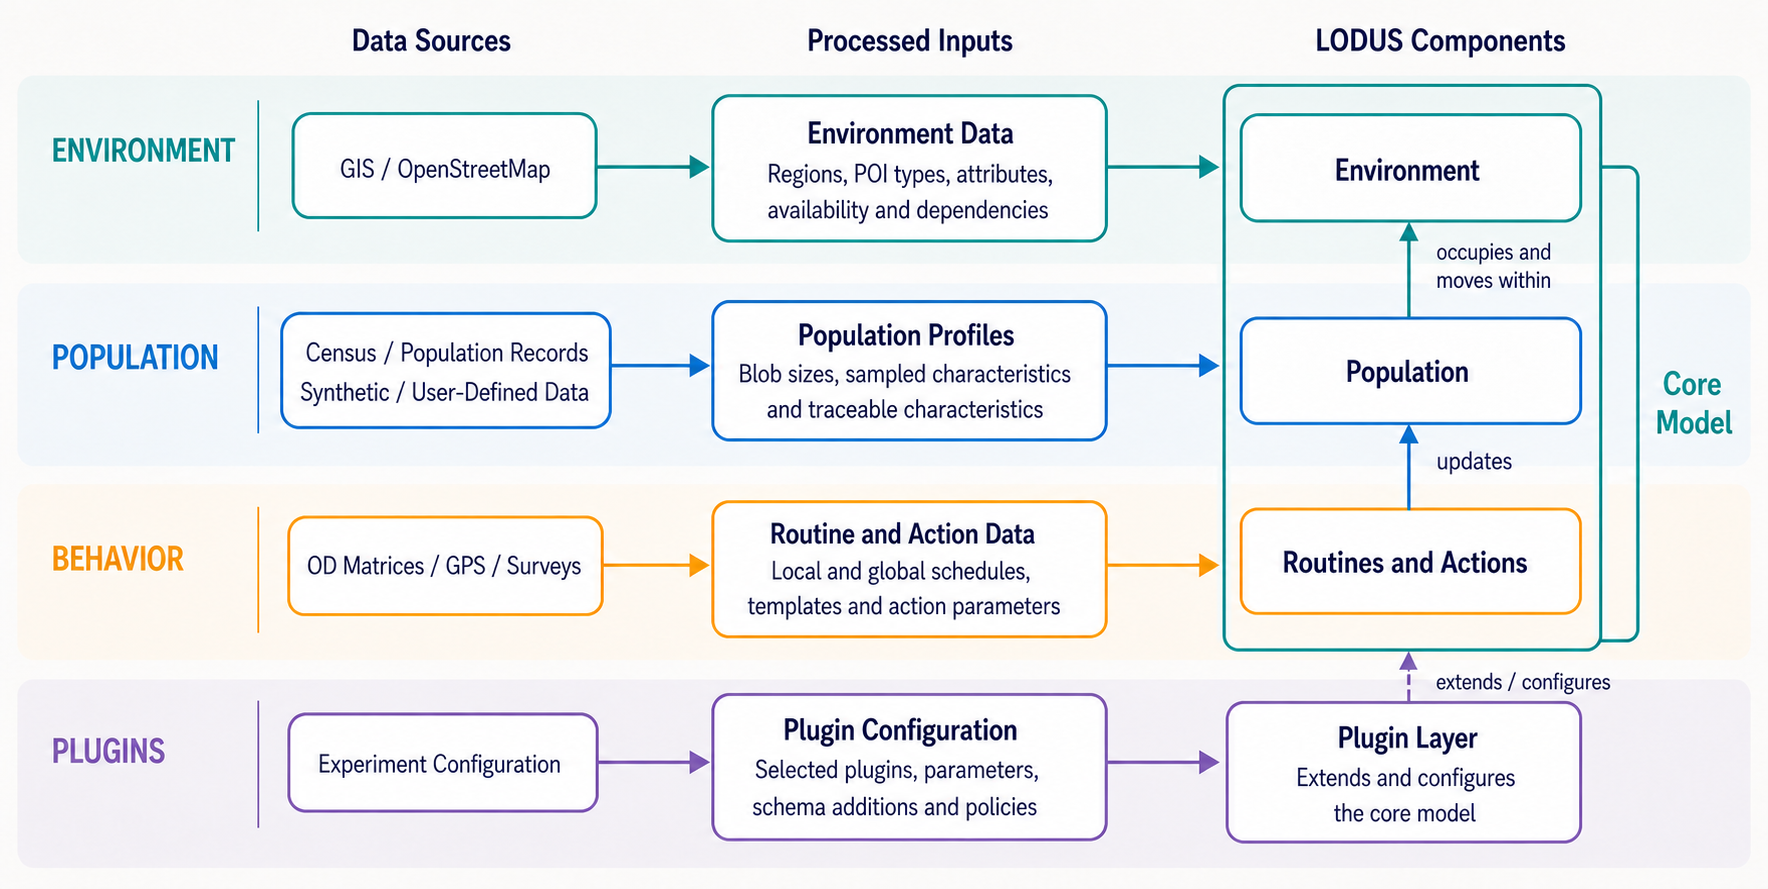
\includegraphics[width=0.98\textwidth]{fig/model/DataDiagramAlternativeCrop.png}
 \caption{Integration of example data sources into LODUS. Geographic, population, mobility, synthetic, and experiment-configuration data are transformed into environment data, population profiles, routine and action definitions, and plugin configurations. These inputs initialize the environment, population, and routines and actions of the core model, while plugins configure and extend the domain-specific characteristics and behavior considered in each experiment.}
 \label{fig:data_diagram}
\end{figure}

%SO: acho que os próximos 3 parágrafos são sobre a fig, né? Eu colocaria itens para ficaar fácil de ver que são sobre as partes da fig
%The population representation draws on aggregation strategies used in macroscopic crowd and mobility models~\cite{thalmann2007crowd,treuille2006continuum}. A LodusPop blob is conceptually related to abstractions such as clouds and legions~\cite{antonitsch2019bioclouds}, but is designed to represent larger and potentially heterogeneous populations. Sampled characteristics retain distributions within a blob, whereas traceable characteristics identify properties shared by its entire population. Population templates can select a subset of a blob according to these characteristics, allowing an action to affect only the relevant population and causing the blob to split when necessary.

%The environment design builds upon the approach introduced by Silva et al.~\cite{silva2020lodus}, while removing dependence on a fixed geographic hierarchy. Regions and points of interest can represent entities at the spatial resolution required by an experiment. Points of interest also have semantic types, extensible attribute mappings, local routines, direct availability conditions, and dependency constraints. They therefore represent not only places occupied by the population, but also the location state and demand that drive simulation behavior.

%This design supports the inversion of responsibility that characterizes LodusPop. Instead of requiring every individual or population group to independently choose a destination, points of interest use routines to request populations with particular profiles. For example, a school may request children during a given period, while a hospital may request patients satisfying a health-state predicate. If a requested location becomes unavailable, the core environment records that condition, while a plugin determines whether the corresponding demand is suppressed, queued, redirected, or otherwise adapted. Domain policies consequently remain explicit extensions rather than implicit properties of the population model.

%SO: ent~~ao :) os items estão abaixo.... será que precisa do texto acima, itens abaixo e mais as subsections abaixo? gosto dos itens e subsections. Não sei se o texto acima é necessário. Se fores tirar, lembra de comentar que a figura representa blabla e será detalhada a seguir. Daí tira esse "remainder" abaixo e já cola com as proximas subsectyions
% GA: comentei acima e resumi
The model is organized into four elements, detailed in the following sections:

\begin{itemize} 
    \item the \textit{environment}, represented by regions and typed points of interest with attributes, local routines, population contents, availability conditions, and dependency constraints; 
    \item the \textit{population}, represented by blobs, sampled and traceable characteristics, population templates, and split and merge operations; 
    \item \textit{routines and actions}, which provide an ordered mechanism for selecting populations and changing the simulation state; and 
    \item \textit{plugins}, which configure and extend the core model with domain-specific characteristics, location attributes, routines, action types, simulation-step updates, observations, and outputs. 
\end{itemize}


\section{Environment}
\label{sec:environment}

To adapt our population mobility simulation to different spatial scopes, we model the environment as an abstract graph composed of \textit{regions} and \textit{points of interest}. The regions ($R$) represent areas of physical space in the virtual world that can contain points of interest ($P$), which represent locations that motivate human travel and that can have population groups (i.e., blobs $B$).
When setting up a simulation, users define the spatial scope that $R$ and $P$ represent. For example, in a city simulation, $R$ could correspond to districts, while $P$ might represent markets, malls, hospitals, residential buildings, and commercial centers.


A region $R$ is represented as a finite set of points of interest $\{P_1,\ldots,P_m\}$. Each point of interest combines a semantic description of the location, its current population, its local behavior, and its availability conditions. We represent $P_i$ as

\begin{equation}
P_i=\bigl(\tau_i,\bm{\alpha}_i,\bm{B}_{P_i},\bm{Ro}_{P_i},\bm{C_i}(t),D_i\bigr),
\label{eq:poi_definition}
\end{equation}

All the parameters are detailed next. %Talvez colar no próximo paragrafo?

%SO: abaixo achei sucinto, type of what? attribute mapping to what??? é a primeira vez que o leitor lê isso, então tem que dar um pouco mais de info.... OU logo abaixo dessa frase tu faz como no exemplo abaixo
%where $\tau_i$ is its type, $\bm{\alpha}_i$ is its attribute mapping, $\bm{B}_{P_i}$ contains the blobs currently located at $P_i$, \bm{Ro}_{P_i}$ is its local routine, $C_i(t)$ contains its active direct disabling conditions at step $t$, and $D_i$ specifies its dependency constraints.%SO: exemplo: All the parameters are detailed next.

%SO: mas, honestamente me parece uma meta explicação.... Tu pdoerias sai da equação e dizer que os parâmetros da equação serão a seguir detalhados e tocar em ficha com o teu proximo txto
%GA: segui esta ideia

The type $\tau_i$ identifies the semantic role of the location, such as \textit{home}, \textit{work}, \textit{school}, \textit{hospital}, or \textit{water source}. Types allow actions to select locations that perform the same role without enumerating them individually. 
%Atributos não tinhamos no paper
%The attribute mapping $\bm{\alpha}_i:K_i\rightarrow V_i$ %SO: o que é K e V? achei ruim essa explicação
%is a mutable finite dictionary of key--value pairs. It stores location-specific information such as coordinates, capacity, an external identifier, or a flood-exposure threshold. %Plugins may declare expected keys and may add, access, or modify their values. An attribute has no framework-wide behavioral meaning unless the core model or a loaded plugin defines its interpretation.
%SO: tirar plugin e pensar sobre attribute mapping
%GA: reescrita abaxo. Daria para simplificar apenas para um "set of attributes"
The attribute mapping $\bm{\alpha}_i:K_i\rightarrow\mathcal{U}_i$ represents a collection of named properties associated with $P_i$. Each key in $K_i$ identifies an attribute whose corresponding value in $\mathcal{U}_i$ describes some property of the point of interest, such as coordinates, capacity, an external identifier, or a flood-exposure threshold. $\mathcal{U}_i$ may contain values of different types, depending on the attribute being represented, and the mapping may be updated during the simulation as these properties change. %Attributes have no intrinsic behavioral meaning unless such meaning is explicitly defined by the model.


% Texto adaptado do que já tinhamos no paper
The components $\bm{B}_{P_i}$ and $\bm{Ro}_{P_i}$ describe the relationship between the location and the simulated population. The former contains the blobs currently occupying $P_i$, while the latter specifies the actions generated by that location over time. 
These components support the inversion of responsibility that characterizes LODUS. In many agent-based approaches, populations decide where to go based on individual preferences or probabilistic rules. Even in field-based models, agents typically remain responsible for sampling and following environmental fields. 
In LODUS, locations instead request populations with particular characteristics. Moving part of the decision logic from individuals to points of interest and regions reduces dependence on granular individual-level movement data and permits aggregated or generalized descriptions of population demand.
 
For example, a market $P_m$ may use $\bm{Ro}_{P_m}$ to request consumers, while $\bm{B}_{P_m}$ represents the population currently at the market. Similarly, a school $P_j$ may use $\bm{Ro}_{P_j}$ to request students, with $\bm{B}_{P_j}$ representing its current population, while a hospital $P_k$ may use $Ro_{P_k}$ to request patients, with $\bm{B}_{P_k}$ representing those currently occupying it. In each case, $\bm{Ro}_{P_i}$ expresses the population demanded by $P_i$, while $\bm{B}_{P_i}$ represents the population currently occupying it.%SO: na frase anterior coloca Ro na routine e B nos blobs apra ficar coerente
%GA: Adicionado

In addition to describing occupation and behavior, a point of interest records whether it is available to participate in simulation actions. Let $\bm{C_i}(t)$ be the set of active direct disabling conditions %SO: será que rules não ficaria mais calro do que "causes"?
%GA: coloquei como conditions. Acho que rules não se encaixa pq C_i em si não descreve as regras, ele só "armazena" informação que diz que o POI foi desativado por tal motivo/plugin.
affecting $P_i$ at step $t$, such as a closure or flood exposure. Each condition is recorded independently. Consequently, removing one condition does not remove any other condition, and $P_i$ is directly available exactly when $\bm{C_i}(t)$ is empty.

Its effective availability may also depend on other points of interest. We represent the dependencies of $P_i$ as

\begin{equation}
D_i=\left\{(k_{ir},\bm{G_{ir}})\right\}_{r=1}^{m_i},
\label{eq}
\end{equation}

where each pair $(k_{ir},\bm{G_{ir}})$ represents one dependency requirement for $P_i$. The set $\bm{G_{ir}}$ contains prerequisite points of interest, and $k_{ir}$ is the minimum number of members of that set that must be available. All requirements in $D_i$ must be satisfied for $P_i$ to be considered available. A mandatory dependency on a single point of interest $P_j$ is represented by $(1,\{{P_j}\})$, while requiring at least $k$ available points from a set $G$ is represented by $(k,G)$.

For example, suppose a pharmacy $P_p$ requires a power source $P_e$ and at least one of two water sources $P_{w_1}$ and $P_{w_2}$. Its dependencies are represented as $D_p={(1,\{{P_e}\}),(1,\{{P_{w_1},P_{w_2}}\})}$. The first requirement makes $P_e$ mandatory, while the second requires at least one of the two water sources to be available. Since all requirements in $D_p$ must be satisfied, the pharmacy requires both an available power source and an available water source.

%GA: reescrevi acima. Mantive a ideia de poder ter mais do que uma regra de dependencia, mas não separei entre "all" e "min". coloquei um exemplo também. 
%SO: abaixo conforme conversamos, tira o all
%where every point of interest in $D_i^{\mathrm{all}}$ 
%SO: acima não entendi. D não é parâmetro de P: como POI in D???? quebrou meu cerebro
%must be available and each pair $(k_g,G_g)$ requires at least $k_g$ available points of interest from $G_g$. The first form represents mandatory dependencies, while the second represents groups of substitutable prerequisites. 
%SO: acima bem confuso. Não sei o que é K e G, e ainda tem o g index

Dependencies may be transitive, so, % effective states are recomputed until no state changes. R
removing one condition from $\bm{C_i}(t)$ cannot enable the point of interest while another condition or an unsatisfied dependency remains. This avoids, for example, reopening a flooded facility merely because its scheduled closure ended.

The availability state of $P_i$ indicates %SO: não entendi esse "Availability records"... parece o nome de um módulo
%GA: Ajustei para falar do ponto de interesse em si, se ele está disponível
whether that location can participate in an action; it does not describe a population response. 
%SO: entendi que até acima tu estavas definindo a tupla do Pi, porque apareceu plugin aqui? Achei aqui bem confuso de acomapnhar
%GA: mudei o trecho abaixo
Changing this state does not itself remove, relocate, or otherwise modify the population at the point of interest. Such changes require explicit actions.
%A plugin may suppress a request from a disabled origin, reject a disabled destination, retain demand in a queue, select a fallback, or reroute it. These alternatives are domain policies and remain outside the core environment definition.


Figure~\ref{fig1:environment} illustrates
regions, typed points of interest, contained blobs, and routines in a LODUS
environment.
Table~\ref{tbl:notation_env} summarizes the notation introduced in this section.
Additionally, Appendix~\ref{app:input} outlines the process of defining the input data necessary for designing a simulation; in particular,  Appendix~\ref{app:input_environment} specifically addresses the data required to model the simulation environment. 

\begin{figure}[ht]
 \centering
  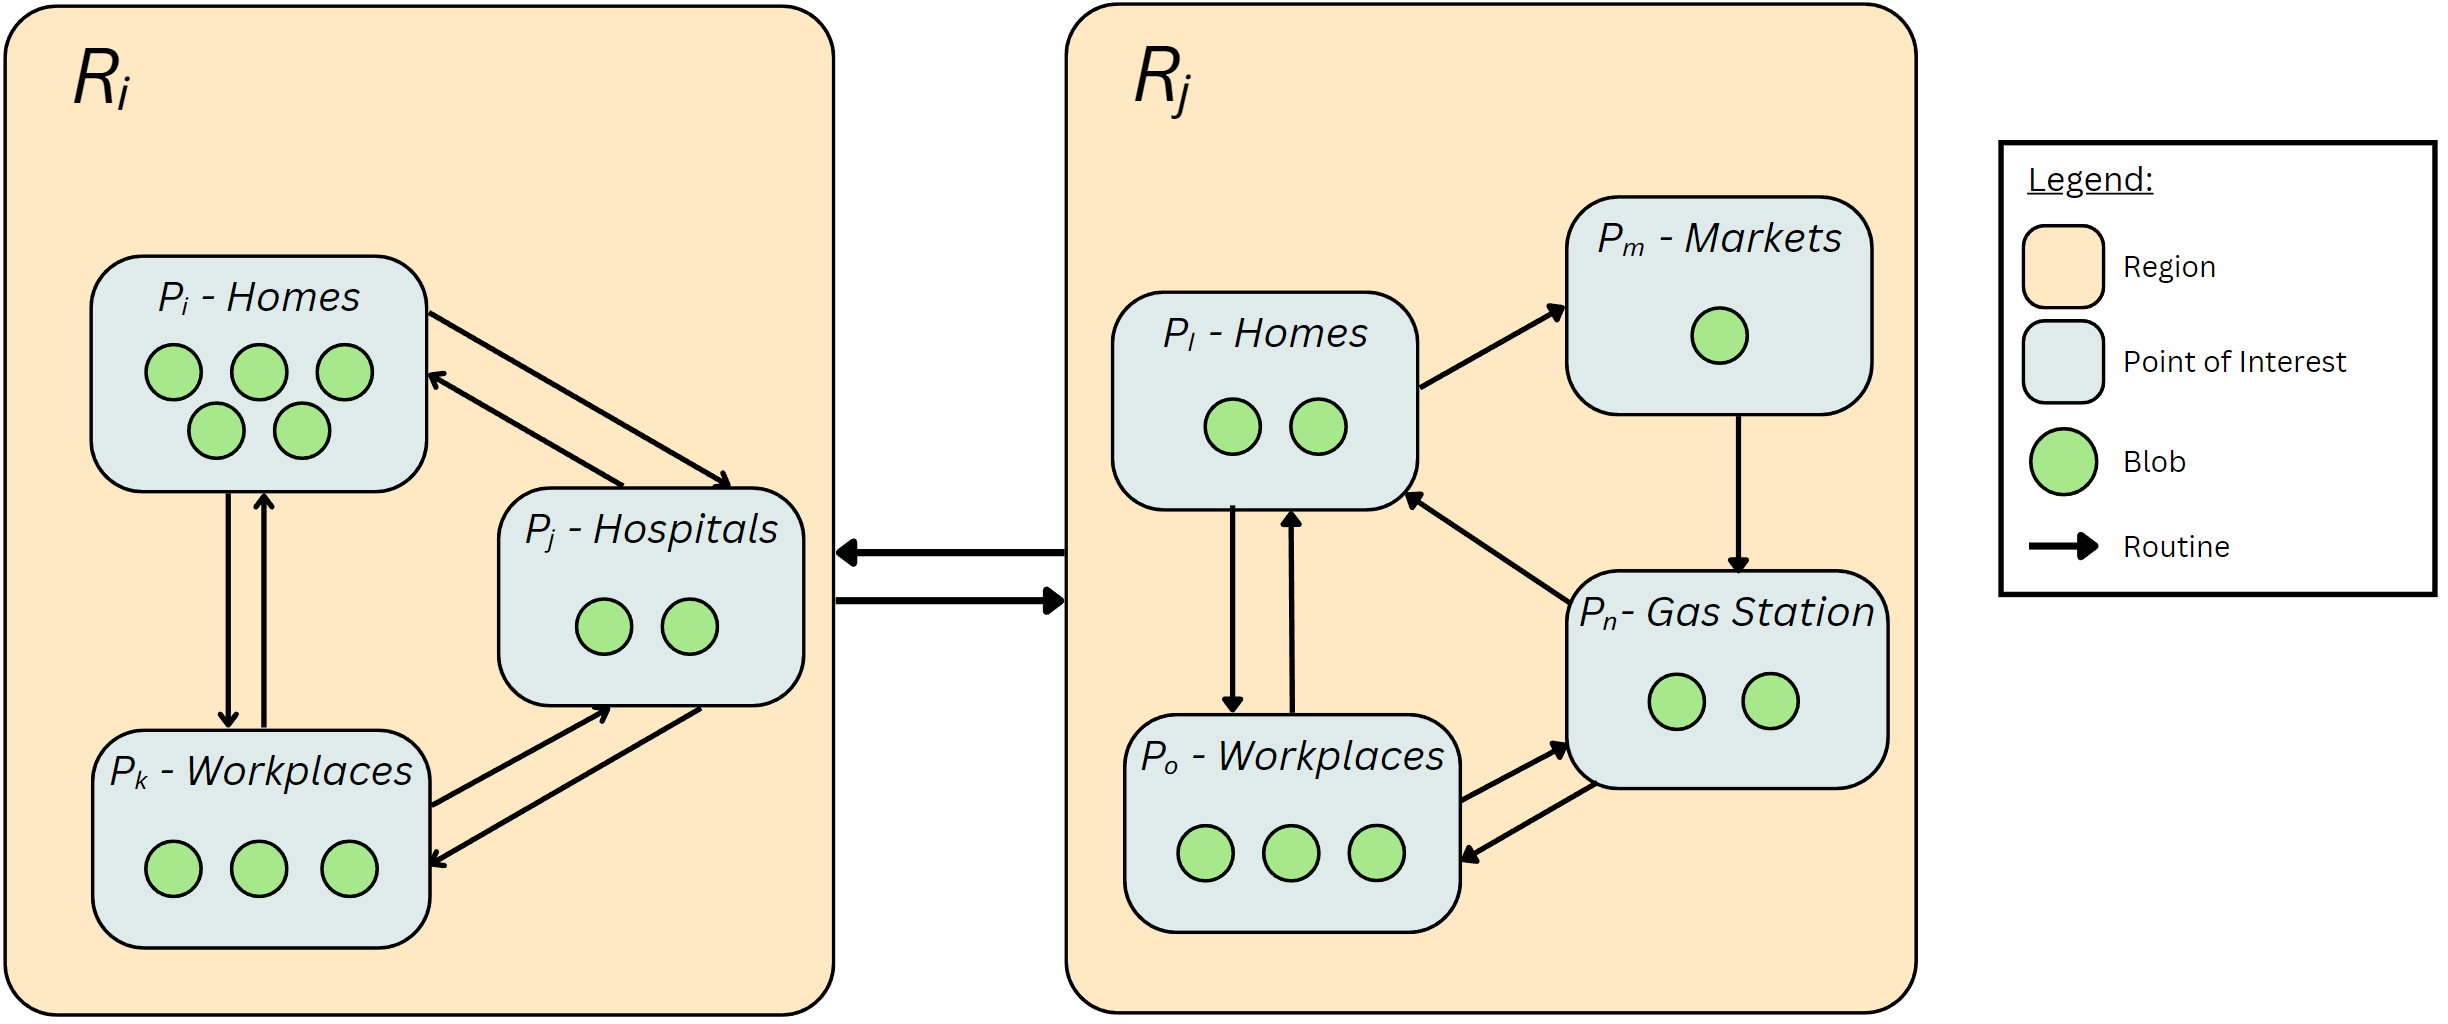
\includegraphics[width=0.98\textwidth]{fig/model/Environment.png}
  \caption{A diagram of a LODUS environment. The figure presents two regions, $R_i$ and $R_j$, containing different points of interest $P$. Each point of interest may contain groups of the population (i.e., blobs), and routines are responsible for moving them in the environment during the simulation.}
  \label{fig1:environment}
\end{figure}

%SO: sobre essa tabela, porque não tem B e RO?
%GA: adicionei
\begin{table}[ht]
\footnotesize
\centering
\caption{Mathematical notation and descriptions of the elements defined in Section~\ref{sec:environment}.}
\label{tbl:notation_env}
\begin{tabularx}{\linewidth}{@{}lcX@{}}
\toprule
\textbf{Element} & \textbf{Notation} & \multicolumn{1}{c}{\textbf{Description}} \\ \midrule
Region & $R$ & Represent areas of physical space in the virtual world that can contain points of interest. A region $R_i$ is defined as a set of $P$. \\ \midrule
\begin{tabular}[c]{@{}l@{}}Point of\\ Interest\end{tabular} & $P$ & Represent locations that the population can occupy as they move during a simulation. A $P_i$ is defined by its type ($\tau_i$), an attribute mapping ($\bm{\alpha}_i$), a collection of population blobs ($\bm{B}_{P_i}$), its local routine ($\bm{Ro}_{P_i}$), its direct disable causes ($\bm{C_i}(t)$), and dependency constraints ($D_i$). \\ \midrule
POI type & $\tau_i$ & Semantic role used to identify locations of the same kind, such as home, work, or school. \\ \midrule
POI attributes & $\bm{\alpha}_i$ & Mapping from named attributes in $K_i$ to their corresponding values in $\mathcal{U}_i$. Values may have different types and may be updated as POI properties change during the simulation. \\ \midrule
Contained blobs & $\bm{B}_{P_i}$ & Collection of population blobs currently located at $P_i$. \\ \midrule
Local routine & $\bm{Ro}_{P_i}$ & Ordered sequence of scheduled actions through which $P_i$ requests population and produces local behavior over time. \\ \midrule
Direct disable causes & $\bm{C_i}(t)$ & Named, independently removable causes that directly prevent $P_i$ from being available at step $t$. \\ \midrule
Dependency constraints & $D_i$ & All-of and minimum-of prerequisite rules used to derive effective availability. \\ %\midrule
%\change{Effective availability} & \change{$e_i(t)$} & %\change{Boolean state obtained from direct causes and the effective states of all prerequisites.} \\ 
\bottomrule
\end{tabularx}
\end{table}

\section{Population}
\label{sec:population}

The population in LODUS is represented by an abstraction of people into blobs $B$, each located at one point of interest at any given simulation step. Blobs describe population groups rather than tracking individuals. A point of interest becoming unavailable does not, by itself, remove or relocate its blobs; any cancellation, waiting, relocation, or redirection of population is performed explicitly by an action according to the policy of the core model or a loaded plugin. 

Formally, a blob is denoted by
\begin{equation}
B=(TP,\bm{Tc},\bm{Sc}),
\label{eq:blob_definition}
\end{equation}
where $TP$ is its total number of individuals, $\bm{Tc}$ is its collection of traceable characteristics, and $\bm{Sc}$ is its collection of sampled characteristics. 

Sampled characteristics ($\bm{Sc}$) represent distributions within the blob. For example, the sampled characteristic \textit{Age} may contain the categories \textit{Child}, \textit{Adult}, and \textit{Elder}, each associated with a number of individuals. Multiple sampled characteristics can jointly describe distributions such as age, schooling level, and employment status. 
%SO: dá um exemplo como fizeste abaixo
%GA: adicionado
For instance, in a blob with $TP=100$, \textit{Age} may contain 20 children, 65 adults, and 15 elders, while \textit{Employment status} may contain 55 employed, 30 unemployed, and 15 student individuals. Each sampled characteristic describes a separate distribution whose category counts sum to $TP$; these marginal distributions do not specify, for example, how many of
the adults are employed.

Traceable characteristics ($\bm{Tc}$) instead store one value for the entire blob. For instance, if \textit{Vaccination status} can be \textit{Vaccinated} or \textit{Unvaccinated}, every individual represented by a particular blob has the same value for that characteristic. 
%SO: será que o traceable lida com personagens com caracteristicas homogeneas e o sampled heetrogeneas?
%GA: a nivel de blob sim, pois a população de uma blob compartilha as mesmas traceable. Mas em nivel de ambiente, as traceables são o que diferenciam as blobs e impedem elas de dar merge.
%The traceable-characteristic schema is simulation-specific. 
% Cola com plugins, talvez remover?
%During initialization, a plugin %SO: Mas, já definimos os plugins???? e essas defs abaixo? sigma... acho que esse texto abaixo está a frente do seu tempo :) TIRAR
%GA: tirado
%may extend it through $E_{\Pi}$ by declaring a characteristic and its default value (Section~\ref{sec:plugins}). The default is applied consistently to the population, after which the characteristic can be read or modified by actions and used as a predicate in population templates.
These characteristics allow us to specify the population in more detail, e.g., elderly people who are currently vaccinated against a given disease or the number of adults who commute to work by bus. Following the previous examples, it becomes possible to track vaccination by age group in the simulation by identifying all blobs $B$ with a \textit{Vaccinated} status and their respective \textit{Age} distributions. Figure~\ref{fig2:blob_diagram} shows the structure of a blob, %SO: quem sabe a blob structure, pois ´bem um diagrama
%GA: ajustado
including its characteristics and associated distributions.

During the simulation, actions generated by the local routine $\bm{Ro}_{P_i}$ may operate on the blobs contained in $P_i$. An action can target a particular population profile, such as children traveling from $P_i$ to a school $P_j$, by applying a population template to the sampled category $Age=Child$.
A population template $T$ specifies which individuals are eligible for an action and the requested quantity. We represent it as

\begin{equation}
T=(T_Q,\bm{T_{Tc}},\bm{T_{Sc}}),
\label{eq:population_template_definition}
\end{equation}

where $T_Q$ is the requested quantity, $\bm{T_{Tc}}$ is an optional set of predicates on traceable characteristics, and $\bm{T_{Sc}}$ is an optional set of predicates on sampled characteristics. Applied to one or more blobs, $T$ filters the eligible population and selects up to $T_Q$ individuals satisfying all declared predicates.


\begin{figure}[ht]
 \centering
  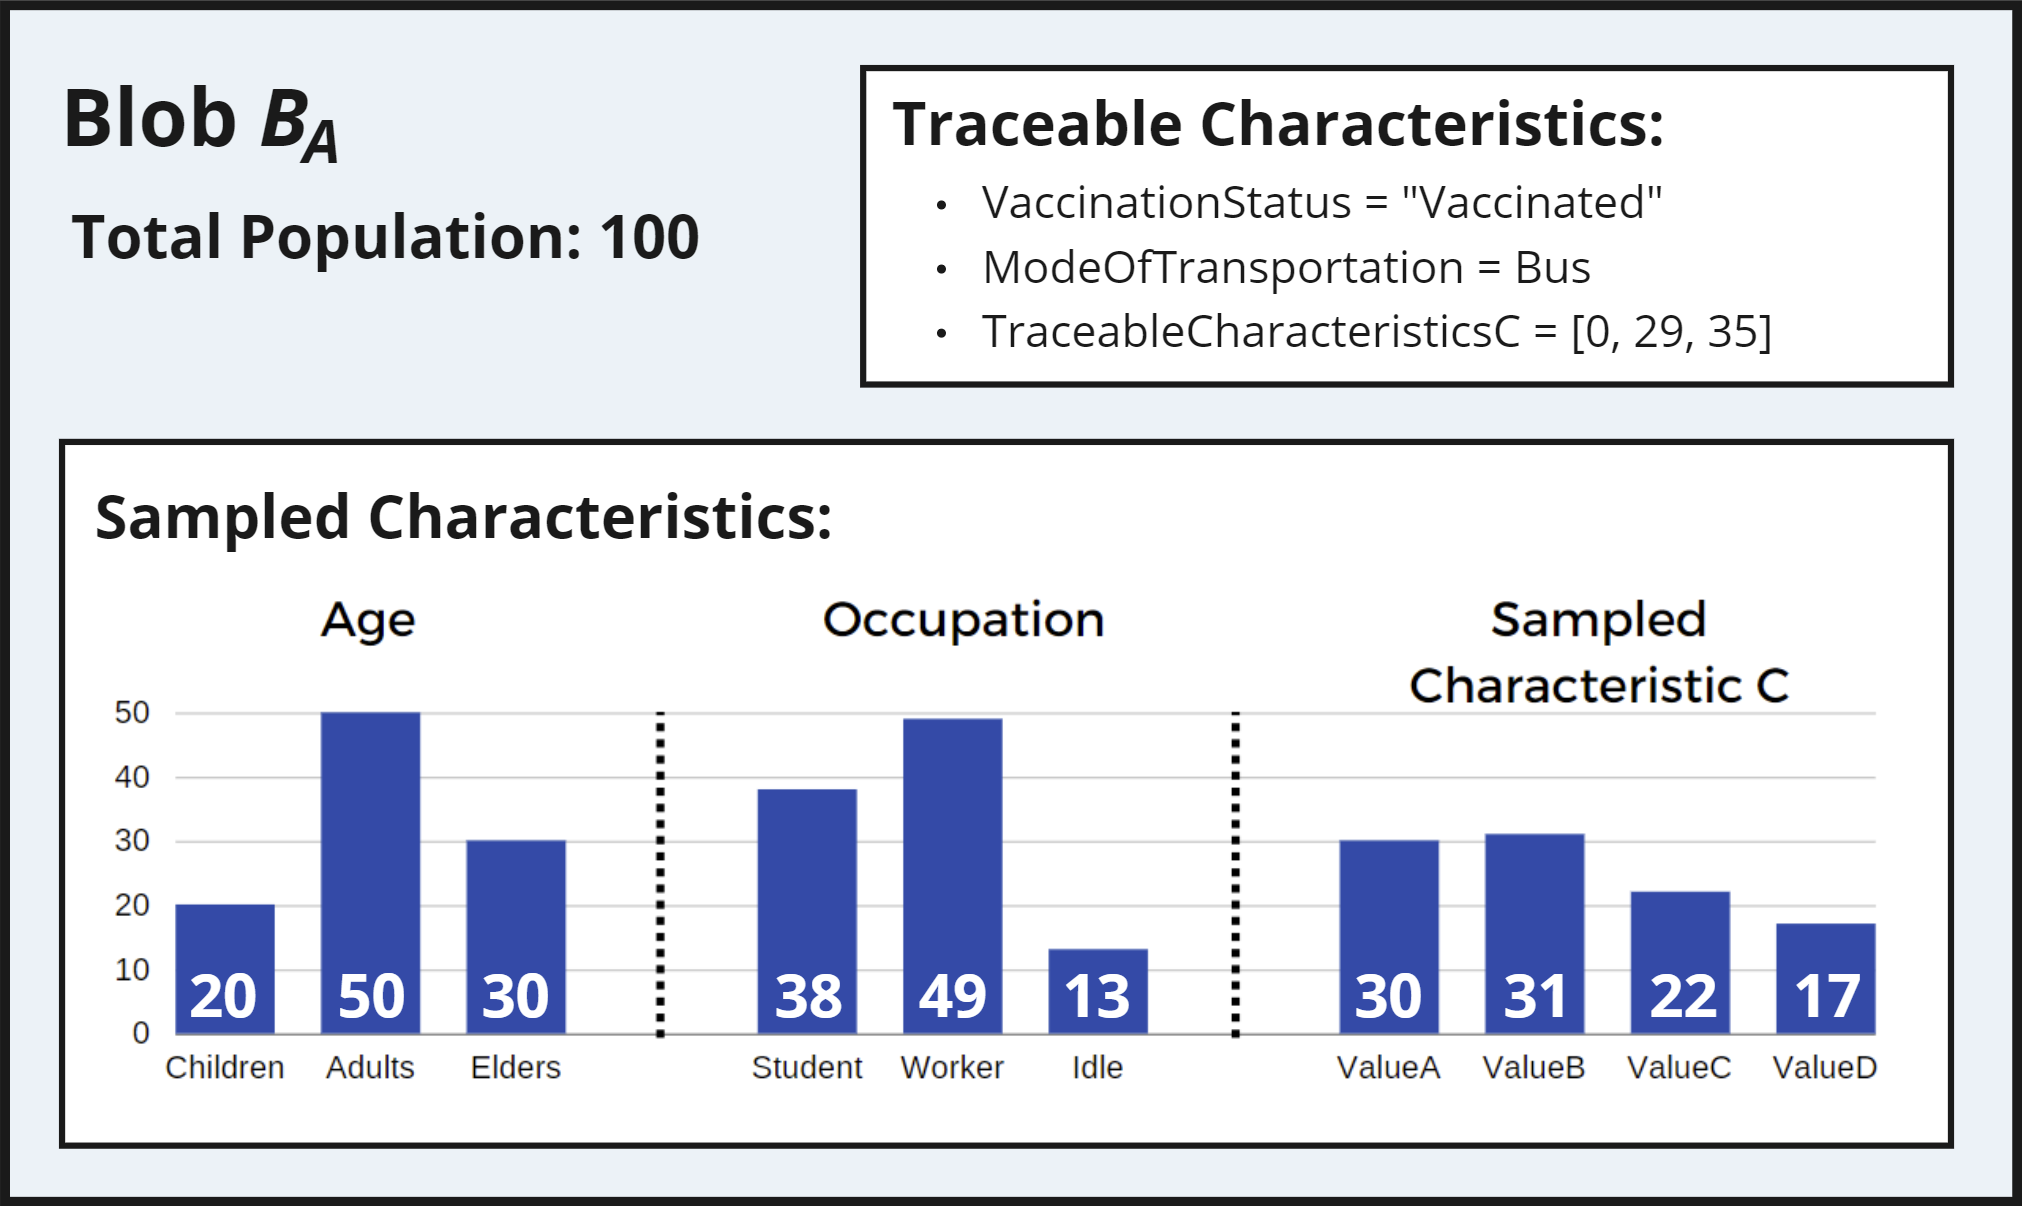
\includegraphics[width=0.9\textwidth]{fig/model/BlobDiagram.png}
  \caption{Structure of a Blob $B_A$ containing 100 people, three traceable characteristics, and three sampled characteristics. Traceable characteristics describe the entire blob population and can have any value type. The distribution of each sampled characteristic sum should be equal to the total population of the blob.} 
  \label{fig2:blob_diagram}
\end{figure}

%SO: abaixo é um exemplo,? então deixa claro
%GA: coloquei um For example,
For example, consider a blob $B_j$ with two sampled characteristics: \textit{i)} \textit{Age}, which includes the possible values \textit{Children}, \textit{Adults}, and \textit{Elders}, and \textit{ii)} \textit{Occupation}, with possible values \textit{Student} and \textit{Worker}. A template $T$ that specifies \textit{Age=Adults} in its collection of sampled characteristics will target only the specified group within $B_j$, in this case, only adults. If the template $T$ does not include a filter for the second sampled characteristic (Occupation), all occupation categories in $B_j$ are affected. The number of affected individuals in categories such as Students and Workers is determined proportionally based on their distribution within $B_j$. For instance, if $B_j$  contains more students than workers, a larger proportion of students will be selected. This process continues until the total number of individuals defined in $T$ is selected or until there are no remaining eligible individuals in $B_j$.

% Splits
When a blob is operated using a population template $T$, it is possible that only a portion of its population may be affected, e.g., a blob $B_i$ that has 75 people and only 20 are selected in $T$. If the operation is to move to another $P$, then such 20 people will create a new blob. This operation generates a split, i.e., the original blob will be separated into two smaller ones. 
In such an example, a template with quantity $T_Q = 20$ selects 20 people from $B_i$ and splits it by creating a new blob $B_j$, which is moved to a different $P$. 
The same occurs when modifying a blob's traceable characteristics ($\bm{Tc}$s). %SO: não é Tsc? 
%GA: não, Tsc são as sampled de um template. Tc são as as traceables de uma blob
For example, another blob $B_k$ has 90 people and a traceable characteristic \textit{InfectionStatus} with value \textit{Healthy}. 20 people are selected, using $T$, to be infected by a disease. The split occurs, and a \textit{InfectionStatus} of $B_l$ (newly created blob) is changed to \textit{Infected}.

% Merge
In addition to split operations, compatible blobs can be merged by combining their total populations $TP$. %SO: TP? Não é TQ? %GA: não, TP é a total population dos blob, TQ é a quantidade pedida por um template
Each sampled characteristic of the resulting blob is obtained by summing the corresponding category counts of the merged blobs. A merge can occur only between blobs in the same point of interest that have equal values for every active traceable characteristic.%, including characteristics introduced by plugins. %SO: tira plugin daqui %GA: done
Consequently, adding a traceable characteristic may also refine the groups that remain distinguishable during merging.
% Figure
Figure~\ref{fig3:blob_operations_with_template} presents a diagram of blobs affected by two templates, resulting in splits and merges. The first scenario, depicted at the top of the figure, demonstrates the relocation of a population. 
The second scenario illustrates changes in traceable characteristics of a population.

%SO: No final desta section citar a tab 1.2 e o apendice
%GA: done
Table~\ref{tbl:notation_pop} summarizes the notation presented in this section. Appendix~\ref{app:input_population} presents an example of the input data required to model the initial population in simulations.

\begin{figure}[ht]
 \centering
  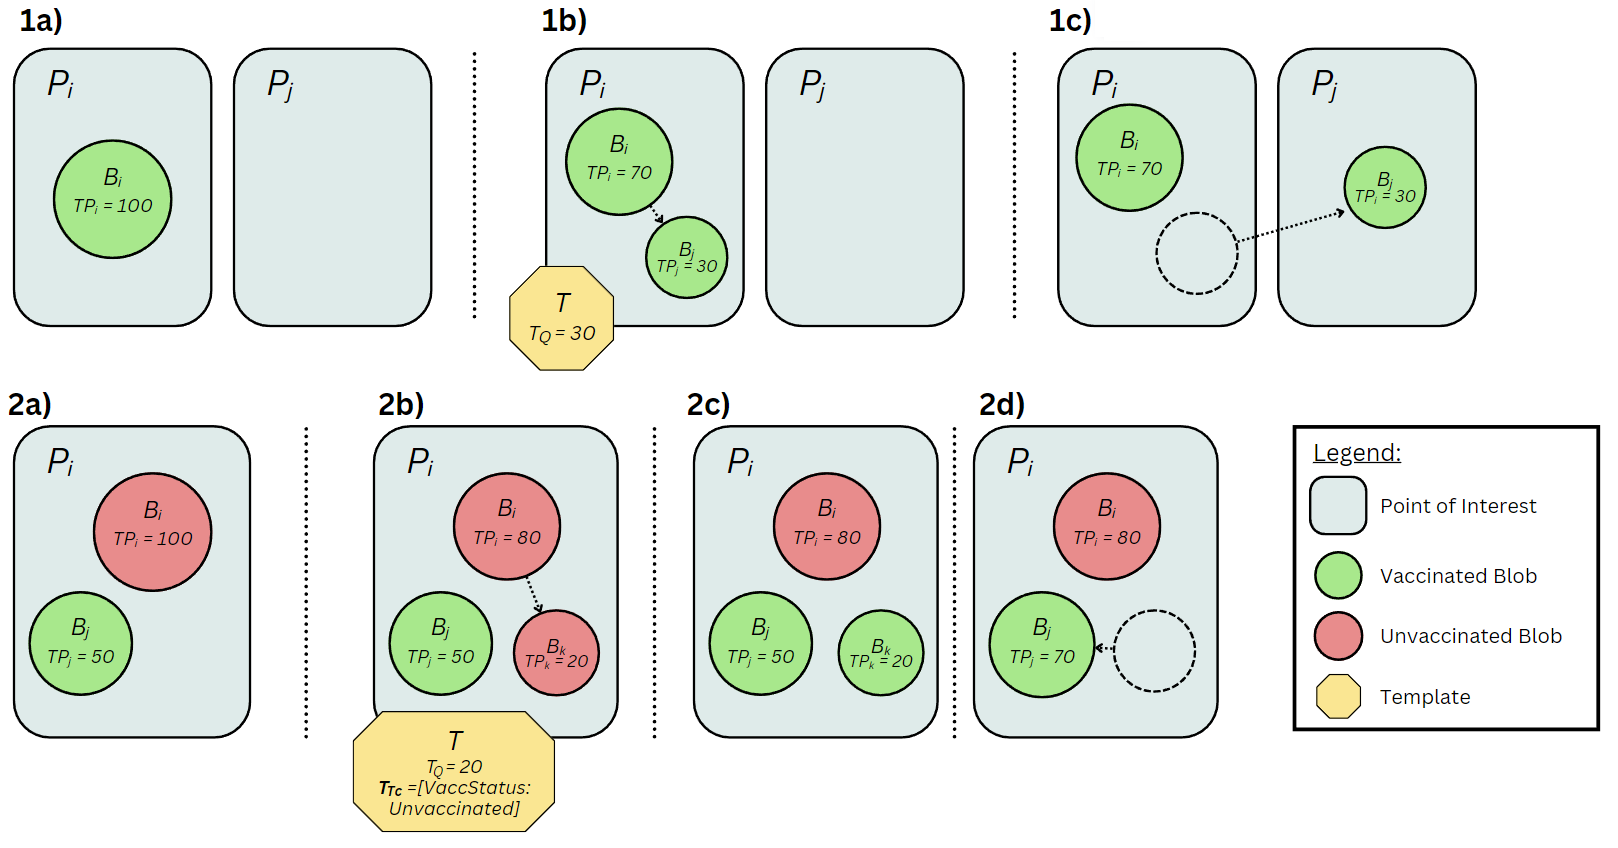
\includegraphics[width=0.99\textwidth]{fig/model/BlobOperations.png}
  \caption{
  Diagram presenting two scenarios of blobs being modified. The first scenario (1) (on the top) shows a population being moved to another location. In 1a, the initial blob $B_i$ has a population of 100. In 1b, a template $T$ selects 30 people, splitting $B_i$ and creating $B_j$. In 1c, $B_j$ is moved to $P_j$. The second scenario (2) shows a population's traceable characteristics changed. In 2a, there are two blobs, $B_i$ containing 100 unvaccinated people (in red), and $B_j$ containing 50 vaccinated people (in green). In 2b, a template $T$ selects 20 unvaccinated people, affecting only $B_i$ and splitting it into $B_k$. In 2c, the traceable characteristic \textit{VaccStatus} of $B_k$ is changed to \textit{Vaccinated}. In 2d, $B_k$ is merged into $B_j$ since they now share the same characteristics and are in the same $P_i$.
  %SO: neste caption achonque podia colocar os nomes das actions MOV e CH
  %GA: Ainda não defini as action até esta hora do texto, mas posso colocar sim
  } 
  \label{fig3:blob_operations_with_template}
\end{figure}

\begin{table}[ht]
\footnotesize
\centering
\caption{Mathematical notation and descriptions of the elements defined in Section~\ref{sec:population}.}
\label{tbl:notation_pop}
\begin{tabularx}{\linewidth}{@{}lcX@{}}
\toprule
\textbf{Element}                                                             & \textbf{Notation} & \multicolumn{1}{c}{\textbf{Description}}                                                                                                                                                                                                                                                                                     \\ \midrule
Blob                                                               & $B$        & Population abstraction $B_i=(TP_i,\bm{Tc}_i,\bm{Sc}_i)$, comprising a total population, traceable characteristics, and sampled characteristics. \\ \midrule
\begin{tabular}[c]{@{}l@{}}Total\\ population\end{tabular} & $TP$ & Number of individuals represented by the blob. \\ \midrule
\begin{tabular}[c]{@{}l@{}}Traceable\\ characteristics\end{tabular} & $\bm{Tc}$ & Collection of identifier--value pairs, each of which has one value shared by the entire blob. \\ \midrule
\begin{tabular}[c]{@{}l@{}}Sampled\\ characteristics\end{tabular} & $\bm{Sc}$ & Collection of categorical distributions over the blob population. For each sampled characteristic, the category counts sum to $TP$. \\ \midrule
\begin{tabular}[c]{@{}l@{}}Population\\ template\end{tabular} & $T$ & Filter $T=(T_Q,\bm{T_{Tc}},\bm{T_{Sc}})$ specifying an eligible population profile and requested quantity for an action. \\ \midrule
\begin{tabular}[c]{@{}l@{}}Requested\\ quantity\end{tabular} & $T_Q$ & Maximum number of eligible individuals requested by the population template. \\ \midrule
\begin{tabular}[c]{@{}l@{}}Traceable-characteristic\\ predicates\end{tabular} & $\bm{T_{Tc}}$ & Optional set of predicates that eligible blobs must satisfy through their traceable characteristics. \\ \midrule
\begin{tabular}[c]{@{}l@{}}Sampled-characteristic\\ predicates\end{tabular} & $\bm{T_{Sc}}$ & Optional set of predicates that select eligible categories from sampled characteristics. \\ \bottomrule
\end{tabularx}
\end{table}

\FloatBarrier


\section{Routines and Actions}
\label{sec:routines}

Behavioral dynamics in LODUS are expressed through routines, which schedule actions at discrete simulation steps. We consider a simulation organized into cycles of fixed length $d$. Let $s\in\mathbb{N}_0$ denote the global simulation-step index. The corresponding step within the current cycle is

\[
t = s \bmod d,
\]

such that $t\in\{0,\ldots,d-1\}$.

A routine is an ordered finite sequence of scheduled actions,

\begin{equation}
Ro=\langle(t_1,A_1),\ldots,(t_n,A_n)\rangle.
\label{eq:routine_definition}
\end{equation}

The ordering is significant when two or more actions share the same cycle step. For each point of interest $P_i$, the local routine $\bm{Ro}_{P_i}$ describes actions requested by that location. The global routine $\bm{GRo}$ has the same structure and schedules actions across the environment rather than being associated with a single point of interest.

Every action retains the common representation

\begin{equation}
A_i=(\kappa_i,T_i,\bm{V}_i),
\label{eq:action_definition}
\end{equation}

%SO: precisas dar um dumping de todas as definições matemáticas e ver se não repetiste nada
where $\kappa_i$ identifies the action type, %SO: N para type é bizarro... 
%GA: mudei para tau, assim como os tipos de pontos de interesse
$T_i$ is a population template, and $\bm{V}_i$ contains the additional parameters required by that action.
Indeed, $\kappa_i$ determines how $T_i$ and $\bm{V}_i$ are interpreted. For population-targeting actions, %SO: como seria N aqui no exemplo? %GA: coloquei um exemplo curto, já que explico em mais detalhe na sequencia
$T_i$ selects the eligible individuals, while an action that does not select a population may ignore an empty template. For example, for a movement action ($\kappa_i=MOV$), $T_i$ may select 20 children and $\bm{V}_i$ specifies the origin and destination points of interest.

In the core model, LODUS provides two built-in action types:
\textit{move population} (MOV), which moves a subset of a blob between points of interest; and \textit{change traceable characteristic} (CH), which modifies the traceable characteristics of a subset of a blob.
A MOV action expects its parameter vector $\bm{V}$ to specify an origin and a destination point of interest. For example, the local routine of $P_i$ may include the pair $(t = 15, A)$, where $A = (MOV, T_i, \bm{V}_i)$, with $T_i=(T_Q=20, T_{Tc}=\emptyset, T_{Sc}=\{Age=Child\})$, and $\bm{V}_i$ encoding $P_i$ as origin and $P_j$ as destination. At cycle step $t = 15$, this action selects 20 children from the blobs at $P_i$, splits them into a new blob, and moves that blob to $P_j$.

A CH action expects $\bm{V}$ to contain the name of a traceable characteristic and its new value. For instance, the local routine of $P_j$ may include $(t = 25, A')$, with $A' = (CH, T_j, \bm{V}_j)$, where $T_j=(T_Q=20, T_{Tc}=\{Status=Unvaccinated\}, T_{Sc}=\emptyset)$, and $\bm{V}_j$ encodes the update ``Status = Vaccinated''. At cycle step $t=25$, this action selects 20 unvaccinated individuals from the blobs at $P_j$, splits them into a new blob, and changes the traceable characteristic Status of that blob to Vaccinated. Figure~\ref{fig3:blob_operations_with_template} illustrates both the movement and characteristic-change scenarios.


% Global routines and Queueing
The same action representation is used by the global routine $\bm{GRo}$. For example, MOV or CH entries in $\bm{GRo}$ may schedule effects across all points of interest at cycle step $t$, enabling global phenomena such as random walks or disease spread. These actions share a scheduling step but are consumed sequentially, not simultaneously. 


To produce repeating temporal behavior, the simulation iterates over cycle steps $t=0,\ldots,d-1$. At cycle step $t$, actions are processed in the following phases:
%SO: eu tirei o s lá de cima que estava confuso. Ver se tem que colocar de volta, mas deixando mais claro. Aqui abaixo fala de plugin
%GA: aqui deve bastar, tirei a parte de plugins de novo
\begin{enumerate}
    \item actions scheduled for cycle step $t$ by $\bm{GRo}$ and each $\bm{Ro}_{P_i}$ are collected;
    \item the collected actions are applied sequentially in their defined order; and
    \item after all actions have been applied, compatible blobs at each point of interest are merged.
\end{enumerate}

%SO: honestamente não vi razão no parágrafo abaixo. Só repetição... podes resumir talvez
%GA: resumido
Before each population-targeting action is applied, its template is evaluated against the current simulation state. Consequently, later actions account for any splits, movements, or characteristic changes produced by preceding actions at the same cycle step.
Figure~\ref{fig:simulation_diagram} illustrates the simulation behavior over one simulation step, and Appendix~\ref{app:simulator} presents an example of the overall simulation control flow.


%SO: mudar a figura, tirar hook, handler e plugin

\begin{figure}[ht]
 \centering
  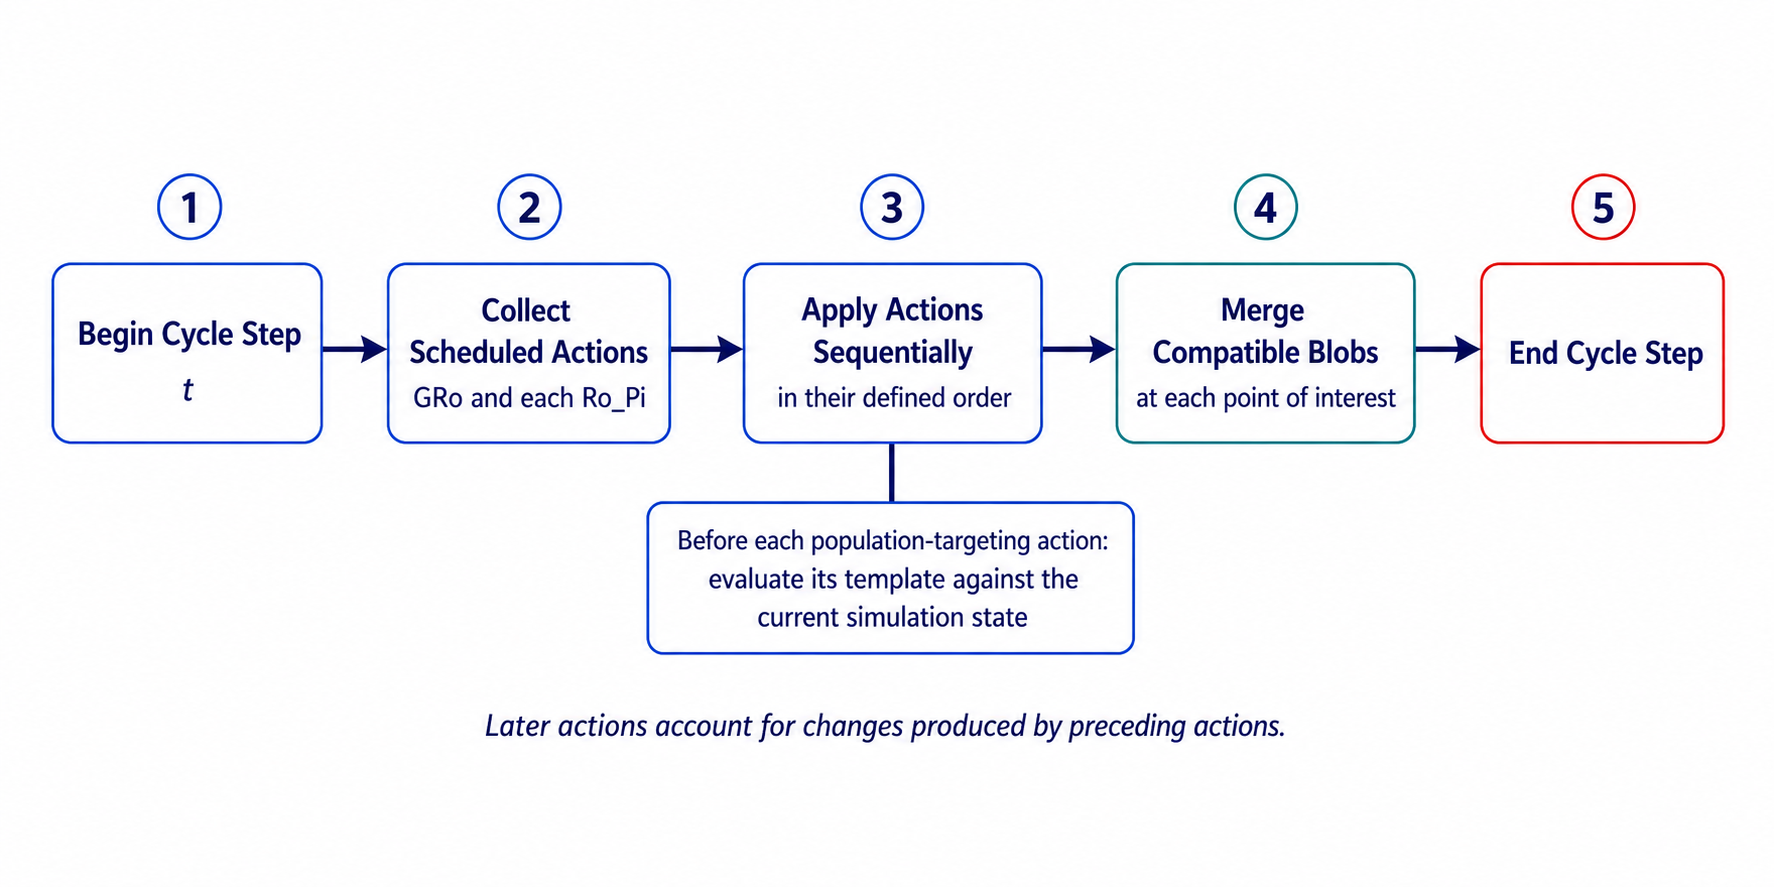
\includegraphics[width=0.99\textwidth]{fig/model/SimulationBehaviorDiagramMethodology.png}
  \caption{Execution flow of one LODUS cycle step. Actions scheduled by the global and local routines are collected and applied sequentially in their defined order. Each action observes the state produced by preceding actions. After all scheduled actions have been applied, compatible blobs at each point of interest are merged.}
  \label{fig:simulation_diagram}
\end{figure}


%GA: deixei o link para o apendice aqui
Table~\ref{tbl:notation_rout} summarizes thee notation presented in this section. Appendix~\ref{app:input_routine} provides an example of the input data used to encode local and global routines.

%SO: trouxe a tabela mais para perto
%GA: coloquei mais para o final pois inclui notações de ações e rotinas
\begin{table}[ht]
\footnotesize
\centering
\caption{Mathematical notation and descriptions of the elements defined in Section~\ref{sec:routines}.}
\label{tbl:notation_rout}
\begin{tabularx}{\linewidth}{@{}lcX@{}}
\toprule
\textbf{Element} & \textbf{Notation} & \multicolumn{1}{c}{\textbf{Description}} \\ \midrule
\begin{tabular}[c]{@{}l@{}}Cycle\\ length\end{tabular} & $d$ & Number of discrete simulation steps in each cycle. \\ \midrule
\begin{tabular}[c]{@{}l@{}}Cycle\\ step\end{tabular} & $t$ & Step within the current cycle, where $0\leq t<d$. \\ \midrule
Routine & $\bm{Ro}$ & Ordered finite sequence $\langle(t_1,A_1),\ldots,(t_n,A_n)\rangle$ of scheduled actions. \\ \midrule
\begin{tabular}[c]{@{}l@{}}Routine\\ entry\end{tabular} & $(t_i,A_i)$ & Action $A_i$ scheduled for cycle step $t_i$. \\ \midrule
\begin{tabular}[c]{@{}l@{}}Local\\ routine\end{tabular} & $\bm{Ro}_{P_i}$ & Ordered routine associated with $P_i$, describing actions requested by that point of interest. \\ \midrule
\begin{tabular}[c]{@{}l@{}}Global\\ routine\end{tabular} & $\bm{GRo}$ & Ordered routine used to schedule actions across the environment rather than at one point of interest. \\ \midrule
Action & $A_i$ & Action $A_i=(\kappa_i,T_i,\bm{V}_i)$, comprising a type, a population template, and additional parameter values. \\ \midrule
\begin{tabular}[c]{@{}l@{}}Action\\ type\end{tabular} & $\kappa_i$ & Identifier that determines how $T_i$ and $\bm{V}_i$ are interpreted. \\ \midrule
\begin{tabular}[c]{@{}l@{}}Population\\ template\end{tabular} & $T_i$ & Template that selects the population eligible for action $A_i$; defined in Section~\ref{sec:population}. \\ \midrule
\begin{tabular}[c]{@{}l@{}}Additional action\\ parameters\end{tabular} & $\bm{V}_i$ & Values required by action type $\kappa_i$, such as origin and destination POIs for MOV. \\ %\midrule
%\begin{tabular}[c]{@{}l@{}}Core action\\ types\end{tabular} & $MOV, CH$ & Move population and change traceable characteristic, respectively. \\ 
\bottomrule
\end{tabularx}
\end{table}

%SO: só a partir daqui pode haver plugin
%GA: deixo este trecho?
%\change{The core action types establish the population-transition semantics shared by all LodusPop simulations. Domain-specific actions, routines, state updates, and observations are introduced through plugins, described in the following section.}


\FloatBarrier
%SO: re-escrevi todo. validar.
\section{Extension Mechanism}
\label{sec:extension_mechanism}

The core model presented in the previous sections defines the structures and behaviors shared by all LODUS simulations: an environment composed of regions and points of interest, a population represented by blobs and population templates, and routines and actions that modify the simulation state over time.

Different application domains, however, may require additional information or behaviors. For example, an epidemic simulation may need to distinguish susceptible and infected populations, a flood simulation may need to associate water-level information with points of interest, and a health-service simulation may require capacity and treatment rules. These elements should not be part of every LODUS simulation.

To support these domain-specific requirements, LODUS adopts an extension mechanism implemented through \emph{plugins}. A plugin augments the core model rather than replacing it. In other words, plugins reuse the same regions, points of interest, blobs, population templates, routines, and actions defined by the core model, while adding only the information and behavior required by a particular simulation. A plugin may extend the core model in one or more of the following ways:

\begin{itemize}
    \item \textbf{Population extensions}, by introducing additional traceable characteristics and their default values. For example, a plugin may add an infection status, vaccination level, or treatment state to the existing blob representation;

    \item \textbf{Environment extensions}, by defining additional point of interest, new attributes or by modifying their state. For example, a flood plugin may interpret a water-level threshold stored in a point of interest and make that location unavailable when the threshold is exceeded;

    \item \textbf{Behavior extensions}, by contributing routines or defining additional action types. These actions follow the same representation $A_i=(\kappa_i,T_i,\bm{V}_i)$ introduced in Section~\ref{sec:routines}, and therefore use the same population-selection and execution mechanisms as the core actions; and

    \item \textbf{Simulation extensions}, by performing domain-specific updates or observations at defined moments of the simulation, such as updating an environmental condition, recording service demand, or collecting experiment-specific outputs.
\end{itemize}

Thus, plugins provide a controlled way of adapting LODUS to different application domains without changing the fundamental abstractions of the model. A simulation is obtained by combining the core model with the set of plugins required by the scenario and by supplying their corresponding parameters.

For consistency with the experimental chapters, the contribution of a plugin $\Pi$ is described using the components summarized in Table~\ref{tbl:notation_plugins} and defined in Equation~\ref{eq:extension}:

\begin{equation}
%\[
\Pi =
\left(
\theta_{\Pi},
E_{\Pi},
R_{\Pi},
F_{\Pi},
H_{\Pi}
\right),
%\]
\label{eq:extension}
\end{equation}


where:

\begin{itemize}
    \item $\theta_{\Pi}$ contains the parameters that configure the plugin for a particular experiment;

    \item $E_\Pi$ represents extensions to the core model, such as additional traceable characteristics or point-of-interest attributes;

    \item $R_{\Pi}$ represents routines or scheduled actions contributed by the plugin;

    \item $F_{\Pi}$ represents additional action types and their execution semantics; and

    \item $H_{\Pi}$ represents optional simulation-step updates, observations, data access, or output recording associated with the plugin.
\end{itemize}

These components are only descriptive categories for organizing plugin contributions; a plugin does not need to provide all of them. 
In many cases, only one or two extensions are required. For instance, a movement-restriction plugin may only provide a parameter and expose its value during the simulation, whereas an epidemic plugin may add a population characteristic and define an action that changes this characteristic.

An important aspect of this design is that domain-specific behavior remains separate from the state represented by the core model. A point of interest, for example, stores its attributes and availability state, but the consequences of becoming unavailable are intentionally left to the application-specific plugins. Depending on the application, a plugin may cancel the corresponding demand, redirect it to another location, place it in a queue, or generate a new action. 
Similarly, blobs retain the same representation regardless of whether they are being used to model mobility, infection, evacuation, or access to health services.

This separation allows the same LODUS model to support different simulation domains while preserving a common representation of population and environment.
The experimental scenarios presented in Chapter~\ref{chapter:experimental_results} illustrate this mechanism by progressively extending the core model with mobility, epidemic, environmental-disruption, shelter, and health-service
behaviors.

\begin{comment}
\section{Extension Mechanism} %SO: mudei o nome
\label{sec:plugins}

%SO: re-escrevi. Valide
The core model presented in the previous sections defines the structures and execution rules common to all LODUS simulations, thereby representing their intrinsic behavior. However, different application domains may require additional behaviors or domain-specific actions. To support such extensions, LODUS adopts an extension mechanism that augments, rather than replaces, the core model by using software components as plugins. So, a simulation is configured by selecting the appropriate set of plugins and their associated parameters. Depending on its purpose, a plugin may introduce new traceable characteristics and their default values, define point-of-interest attributes, contribute routines, define additional action types, trigger or generate actions, provide domain-specific data, or record simulation outputs.

%The core model, as presented in the last sections, represents the structures and execution rules shared by all simulations, i.e., the innate behavior of all simulation in LODUS. However, depending on the simulation to be designer, other actions or behaviors can be necessary. To acomplish with that, we propose the plugins which aimjs to provide the behavior required for a particular application domain. Plugins extend rather than replace points of interest, blobs, population templates, routines, and actions. A new simulationt selects a set of plugins and supplies their parameters. Depending on its role, a plugin may add traceable characteristics and their defaults, define conventions for point-of-interest attributes, contribute routines, register new action types, invoke or emit other actions, expose data services, or record outputs.

Let $\mathcal{S}(s)$ denote the complete simulation state at simulation step $s$, 
%SO: ver se s index não é t
including points of interest, blobs, routines, availability states, and action registries. 
A plugin $\Pi$ is defined through the extension contract

% Notação sugerida por IA com base na implementação de plugins
\begin{equation}
\Pi=\left(\bm{\theta}_{\Pi},E_{\Pi},\mathcal{R}_{\Pi},
\mathcal{F}_{\Pi},\mathcal{H}_{\Pi}\right),
\label{eq:plugin_definition}
\end{equation}

where:
\begin{itemize}
    \item $\bm{\theta}_{\Pi}$ is a finite key--value mapping of parameters read from the experiment configuration;
    %SO: não entendi o que é esse parãmtro, para que serve
    \item $E_{\Pi}$ contains optional additions to the model vocabulary, including declarations and defaults for traceable characteristics and point-of-interest attribute conventions; %SO: mas porque delta? por causa do additions? isso é viagem do gpt
    \item $\mathcal{R}_{\Pi}$ is an optional finite collection of local-routine, global-routine, start-of-step, or end-of-step action contributions;
    %SO: deveria ser um vetor então?
    \item $\mathcal{F}_{\Pi}=\{(N,f_N)\}$ is an optional registry associating action-type identifiers with the handlers that consume them; and
    %SO: tu já não tens action type e "handlers"?
    \item $\mathcal{H}_{\Pi}$ defines the optional extension points associated with the simulation lifecycle, time-step execution, data access, observation, and output recording.
    %\item $\mathcal{H}_{\Pi}$ contains optional lifecycle, time-step,
    data-access, observation, and logging hooks.
\end{itemize}

Any component may be empty, and a plugin need only use the extension points required by its role. %The notation consequently covers action, routine, logger, and data plugins without requiring each plugin to implement every mechanism.
At load time, the simulator reads $\bm{\theta}_{\Pi}$, applies the declarations in $E_{\Pi}$, incorporates $\mathcal{R}_{\Pi}$, registers $\mathcal{F}_{\Pi}$, and activates $\mathcal{H}_{\Pi}$. 
During execution, each registered pair $(N,f_N)$ associates an action identifier $N$ with the handler that consumes actions of that type. 
Plugin actions retain the common action structure $A=(N,T,\bm{V})$, so their handlers receive the same population template and additional values used by core actions. At a high level, a handler is described as

\begin{equation}
f_N:\bigl(\mathcal{S}(s),T,\bm{V},t,s;\bm{\theta}_{\Pi}\bigr)
\longmapsto
\bigl(\mathcal{S}'(s),\langle A_1,\ldots,A_\ell\rangle\bigr).
\label{eq:plugin_action_handler}
\end{equation}

% Ações simples e complexax
A primitive handler applies its transition directly to $\mathcal{S}$ and may return an empty action sequence. A composite handler may instead return core or plugin-defined actions, which are consumed through the same $A=(N,T,\bm{V})$ contract. This makes calls to other actions explicit while preserving population-template selection and sequential execution.

The lifecycle and observation hooks in $\mathcal{H}_{\Pi}$ allow a plugin to update the simulation at step boundaries, expose data to other plugins, record state, and release its resources. 
% Abaixo, plugins que dependem de outros plugins
A loaded set of plugins $\mathbb{P}=\{\Pi_1,\ldots,\Pi_r\}$ is valid when its action identifiers and schema declarations are compatible and all plugin requirements are present.
%Dependencies between plugins must be stated by the experiment; for example, a mobility plugin may require an action type provided by a population-gathering plugin. 
%Appendix~\ref{app:plugin} illustrates the implementation of such an extension.

The same definition provides a reporting template for the experimental chapters:

\begin{equation}
\Pi_x=(\bm{\theta}_x,\Delta\Sigma_x,\mathcal{R}_x,
\mathcal{F}_x,\mathcal{H}_x).
\label{eq:experiment_plugin_template}
\end{equation}

An experiment need only describe the nonempty components and the scenario values of $\bm{\theta}_x$. For example, a dialysis plugin can state its capacity and service parameters in $\bm{\theta}_x$, patient-state characteristics in $\Delta\Sigma_x$, scheduled requests in $\mathcal{R}_x$, and service handlers and update hooks in $\mathcal{F}_x$ and $\mathcal{H}_x$.

% Diferença de informações de POIs vs Plugins acessando e modificando o comportamento base
Point-of-interest state and plugin behavior remain distinct. The tuple $P_i$ defines where location data are stored and how effective availability is derived. The tuple $\Pi$ defines the experiment-specific rules that read or modify that state and determine the population response. 
For example, a flood plugin may compare a forcing value with a threshold in $\bm{\alpha}_i$ and add a cause to $C_i(t)$. The dependency constraints $D_i$ then propagate effective unavailability, after which a mobility or service plugin decides whether the resulting demand is canceled, queued, or redirected. Service capacities, queues, flood thresholds, patient stays, destination substitution, and commute lifecycles consequently remain explicit plugin policies rather than universal fields of every blob or point of interest.


\begin{table}[ht]
\footnotesize
\centering
\caption{Mathematical notation and descriptions of the plugin extension contract.}
\label{tbl:notation_plugins}
\begin{tabularx}{\linewidth}{@{}lcX@{}}
\toprule
\textbf{Element} & \textbf{Notation} & \multicolumn{1}{c}{\textbf{Description}} \\ \midrule
Plugin & $\Pi$ & Extension contract $(\bm{\theta}_{\Pi},E_{\Pi},\mathcal{R}_{\Pi},\mathcal{F}_{\Pi},\mathcal{H}_{\Pi})$. \\ \midrule
Configuration & $\bm{\theta}_{\Pi}$ & Experiment-supplied parameter mapping. \\ \midrule
Schema additions & $E_{\Pi}$ & Population characteristics, defaults, and POI-attribute conventions introduced by the plugin. \\ \midrule
Routine contributions & $\mathcal{R}_{\Pi}$ & Local, global, start-of-step, or end-of-step actions contributed by the plugin. \\ \midrule
Action registry & $\mathcal{F}_{\Pi}$ & Pairs $(N,f_N)$ associating action identifiers with consuming handlers. \\ \midrule
Hooks and services & $\mathcal{H}_{\Pi}$ & Lifecycle, time-step, data-access, observation, and logging interfaces. \\ \bottomrule
\end{tabularx}
\end{table}


\begin{table}[ht]
\footnotesize
\centering
\caption{Mathematical notation describing the contributions of a LodusPop plugin.}
\label{tbl:notation_plugins}
\begin{tabularx}{\linewidth}{@{}lcX@{}}
\toprule
\textbf{Element} & \textbf{Notation} & \multicolumn{1}{c}{\textbf{Description}} \\ \midrule

Plugin &
$\Pi$ &
Plugin contribution described by $(\bm{\theta}_{\Pi},E_{\Pi},\mathcal{R}_{\Pi},\mathcal{F}_{\Pi},\mathcal{H}_{\Pi})$. \\ \midrule

Configuration &
$\bm{\theta}_{\Pi}$ &
Experiment-specific parameters used to configure the plugin. \\ \midrule

Model extensions &
$E_{\Pi}$ &
Additional traceable characteristics, point-of-interest attributes, or other domain-specific elements introduced into the core model. \\ \midrule

Routine contributions &
$\mathcal{R}_{\Pi}$ &
Additional routines contributed by the plugin. \\ \midrule

Action extensions &
$\mathcal{F}_{\Pi}$ &
Additional action types together with their execution semantics. \\ \midrule

Simulation extensions &
$\mathcal{H}_{\Pi}$ &
Simulation-step updates, observations, data access, or output recording contributed by the plugin. \\

\bottomrule
\end{tabularx}
\end{table}
\end{comment}

\begin{table}[ht]
\footnotesize
\centering
\caption{Mathematical notation describing the contributions of a LODUS plugin.}
\label{tbl:notation_plugins}
\begin{tabularx}{\linewidth}{@{}lcX@{}}
\toprule
\textbf{Element} & \textbf{Notation} & \multicolumn{1}{c}{\textbf{Description}} \\ 
\midrule

Plugin &
$\Pi$ &
Plugin contribution described by $(\theta_{\Pi},E_{\Pi},R_{\Pi},F_{\Pi},H_{\Pi})$. \\ 
\midrule

Configuration &
$\theta_{\Pi}$ &
Experiment-specific parameters used to configure the plugin. \\ 
\midrule

Model extensions &
$E_{\Pi}$ &
Additional traceable characteristics, point-of-interest attributes, or other domain-specific elements introduced into the core model. \\ 
\midrule

Routine contributions &
$R_{\Pi}$ &
Additional routines or scheduled actions contributed by the plugin. \\ 
\midrule

Action extensions &
$F_{\Pi}$ &
Additional action types together with their execution semantics. \\ 
\midrule

Simulation extensions &
$H_{\Pi}$ &
Simulation-step updates, observations, data access, or output recording associated with the plugin. \\

\bottomrule
\end{tabularx}
\end{table}

%\FloatBarrier

% ---------------------------------------------------------------------------
% Definições alternativas para plugins (sugestões de IA)
% ALTERNATIVE PLUGIN DEFINITION 2 (compact transition-operator view)
% This option treats a configured plugin as one operator over state and pending
% actions. It is compact, but hides which extension mechanisms an experiment uses.
% \[
% \Pi_{\bm{\theta}}:\mathcal{S}\times A^{*}\longrightarrow
% \mathcal{S}\times A^{*}.
% \]
% The operator may transform state, consume actions, and emit actions. Setup,
% routine injection, logging, and schema changes would require separate prose.

% ALTERNATIVE PLUGIN DEFINITION 3 (base-model delta view)
% This option defines a plugin by the changes it contributes to a base simulator.
% It emphasizes composition, but is less convenient for parameters and stateful
% hooks in an experimental specification.
% \[
% \Pi=(\Delta\Sigma,\Delta Ro,\Delta F,\Delta H),
% \qquad M_{\Pi}=M_0\oplus\Pi.
% \]
% Here \Delta\Sigma extends the schema, \Delta Ro extends routines, \Delta F
% extends the action registry, and \Delta H extends lifecycle and observation
% hooks. Parameters would be supplied separately as \Pi_{\bm{\theta}}.
% ---------------------------------------------------------------------------

\chapter{Simulation Environments, Plugins, and Input Data}
\label{sec:simulation_environments_and_data}



LODUS is designed to model simulation scenarios using real-world spatial and demographic data. 
To evaluate this capability in an urban setting, we model the city of Porto Alegre and its population using three main representations. 
The first represents both population and points of interest ($P$s) at the neighborhood level. The second preserves neighborhoods as simulation regions while representing population and $P$s at the finer census-sector level across the entire city. The third uses the same census-sector-level representation but is restricted to 13 neighborhoods in the central area of Porto Alegre. 

In addition to environment and population data, service, flood, shelter, and behavioral datasets are overlaid on the representation appropriate to each use case. This chapter presents these environments and their shared inputs, distinguishing between observed or externally sourced data, data derived through spatial or statistical preprocessing, and values configured specifically for each simulation scenario.

%SO: re-escrevi. validar
%GA: validado
Following the model introduced in Chapter~\ref{chapter:proposed_model}, each input described in this chapter contributes either to the initialization of the core model or to the configuration of domain-specific plugins.
Core inputs define the simulation environment, the initial population, and the routines executed during the simulation. 
Plugin-specific inputs instead configure the parameters of a plugin, extend the core model with application-specific information, or provide the data required by the additional routines, actions, or simulation behaviors introduced by that plugin. 
This distinction separates the origin of an input from its role in the simulation, making it possible to reuse the same core model across different application domains.

%Following the definitions introduced in Chapter~\ref{chapter:proposed_model}, each input described in this chapter has one of two roles. Core inputs initialize point-of-interest types and attributes, population blobs and their characteristics, or local and global routines. Experiment-specific inputs instead configure plugins through $\bm{\theta}_{\Pi}$, extend the model vocabulary through $E_{\Pi}$, or provide data used by routine contributions, action handlers, and lifecycle hooks. This distinction separates the provenance of an input from the mechanism through which it affects the simulation.



\section{Spatial Representations}
\label{sec:spatial_representations}

Following the environment definition introduced in Section~\ref{sec:environment}, neighborhoods are modeled as simulation regions ($R$), each containing a set of $P$s. The environments differ primarily in their spatial extent and in the resolution at which population and $P$s are represented.


\subsection{Neighborhood-Level Environment}
\label{sec:neighborhood_level_environments}

The neighborhood-level Porto Alegre model follows the environment described in the published manuscript~\cite{silva2026lodusPop}. Each of the city's 94 neighborhoods is represented as a simulation region. 
Neighborhood boundaries were obtained from digital cartographic data published by Porto Alegre City Hall\footnote{Porto Alegre City Hall digital maps, including the neighborhood boundary layer (``Bairros (LC 12.112/16)''): \url{https://prefeitura.poa.br/carta-de-servicos/mapas-digitais-da-smamus}.}, while OpenStreetMap was used to obtain coordinates for urban amenities represented as $P$s\footnote{OpenStreetMap: \url{https://www.openstreetmap.org/}.}. 
Each region contains one $P$ of each standard type $\tau_i$: \textit{home}, \textit{work}, \textit{school}, \textit{marketplace}, \textit{pharmacy}, and \textit{gas station}.
Selected regions also contain $P$s with specialized types, such as shopping malls and stadiums, when required by an experiment. Coordinates, external identifiers, and other location-specific values are stored in the attribute mapping $\bm{\alpha}_i$ of each $P_i$.


Population totals, citywide occupation proportions, and the citywide age distribution were obtained from the 2010 Census of the Brazilian Institute of Geography and Statistics (IBGE)\footnote{IBGE city profile for Porto Alegre: \url{https://cidades.ibge.gov.br/brasil/rs/porto-alegre/panorama}.}. Neighborhood-level population and age distributions were complemented with municipal information published by ObservaPOA and PROCEMPA\footnote{ObservaPOA: \url{http://www.observapoa.com.br/}. PROCEMPA's Porto Alegre em Análise portal: \url{https://portoalegreemanalise.procempa.com.br/}.}.


One initial population blob is placed at the home $P$ of each neighborhood. Age and occupation are represented as sampled characteristics in $\bm{Sc}$, since each blob stores a distribution over their categories. Experiment-specific traceable characteristics, such as infection status, vaccination status, mobility lifecycle, or patient state, are introduced by the corresponding plugin through its model extensions ($E_{\Pi}$), which also define their
default values.

Occupation is divided into \textit{students}, \textit{workers}, and \textit{others}. Because neighborhood-level occupation distributions were unavailable, the same citywide distribution was applied to every neighborhood: approximately 21.6\% students, 54.7\% workers, and 23.7\% others. Age is divided into four categories: \textit{child} (0--14 years), \textit{young} (15--24 years), \textit{adult} (25--59 years), and \textit{elder} (60+ years). Each neighborhood uses its corresponding age distribution, while the overall modeled population consists of approximately 18.7\% children, 15.7\% young people, 50.5\% adults, and 15.1\% elders. Overall, the neighborhood-level environment comprises 94 $R$s, 504 $P$s, and a total population of 1,409,351.

\subsection{Census-Sector-Level Environments}
\label{sec:census_sector_environments}

The more detailed environments use census sectors, also referred to as enumeration areas, as the spatial unit for population initialization. Neighborhoods remain the simulation regions, preserving compatibility with region-level routines and outputs, while census sectors provide a finer spatial representation of the population and associated $P$s. Official census-sector aggregates and geographic files were obtained from the 2022 IBGE Census\footnote{IBGE 2022 Census sectors: \url{https://www.ibge.gov.br/geociencias/organizacao-do-territorio/malhas-territoriais/26565-malhas-de-setores-censitarios-divisoes-intramunicipais.html}.}.

The neighborhood-level environment described in the previous section was originally constructed using demographic data from the 2010 IBGE Census, consistent with the environment used in the published experiments~\cite{silva2026lodusPop}. The census-sector environments were subsequently constructed using the more recent 2022 Census data. %Consequently, differences in population totals between these environments reflect both their spatial representation and the underlying census datasets.


In both census-sector environments, six standard $P$s are instantiated for each census sector within the neighborhood region containing that sector. Their types ($\tau_i$) correspond to \textit{home}, \textit{work}, \textit{school}, \textit{marketplace}, \textit{pharmacy}, and \textit{restaurant}. The census sector is therefore the unit used to position and initialize these $P$s, whereas neighborhoods remain the simulation regions ($R$s). The population associated with each sector is initially represented by a blob at its corresponding \textit{home} $P$.

We consider two versions of this representation: a \textit{complete environment}, covering all 94 neighborhoods of Porto Alegre, and a \textit{reduced environment}, restricted to 13 neighborhoods in the central area of the city.
The complete environment applies this representation to 2,711 census sectors distributed across all 94 neighborhoods, resulting in 16,266 $P$s and a total population of 1,331,414. The reduced environment applies the same representation to 435 census sectors distributed across 13 central neighborhoods, resulting in 2,610 $P$s and a total population of 159,886.


Table~\ref{tbl:shared_simulation_environments} summarizes the three environment versions. The reported counts of $P$s refer to the base spatial representations. Domain-specific plugins may extend these environments with additional $P$s required by a scenario, such as shelters, dialysis clinics, and water-treatment facilities.
Figure~\ref{fig:spatial_representations} presents their spatial representations, highlighting the distribution of home $P$s. 
The main use cases are presented in the results chapter (Chapter~\ref{chapter:experimental_results}).

\begin{table}[ht]
\centering
\footnotesize
\setlength{\tabcolsep}{4pt}
\caption{Base Porto Alegre spatial representations used by the experiments.}
\label{tbl:shared_simulation_environments}
\begin{tabularx}{\linewidth}{@{}p{2.6cm}rrrrX@{}}
\toprule
\textbf{Environment} &
\textbf{Regions} &
\textbf{Home $P$s} &
\textbf{Base $P$s} &
\textbf{Population} &
\textbf{Main use cases} \\
\midrule
Neighborhood-level
    & 94 & 94 & 504 & 1,409,351
    & Published L\'evy Walk, large-scale events, epidemic contagion, and vaccination. \\
Reduced census-sector
    & 13 & 435 & 2,610
    & 159,886
    & Popular Times, L\'evy Walk, dialysis, and flood-aware mobility. \\
Complete census-sector 
    & 94 & 2,711 & 16,266
    & 1,331,414
    & Popular Times, L\'evy Walk, dialysis, and flood-aware mobility. \\
\bottomrule
\end{tabularx}
\end{table}

\begin{figure}[ht]
 \centering
  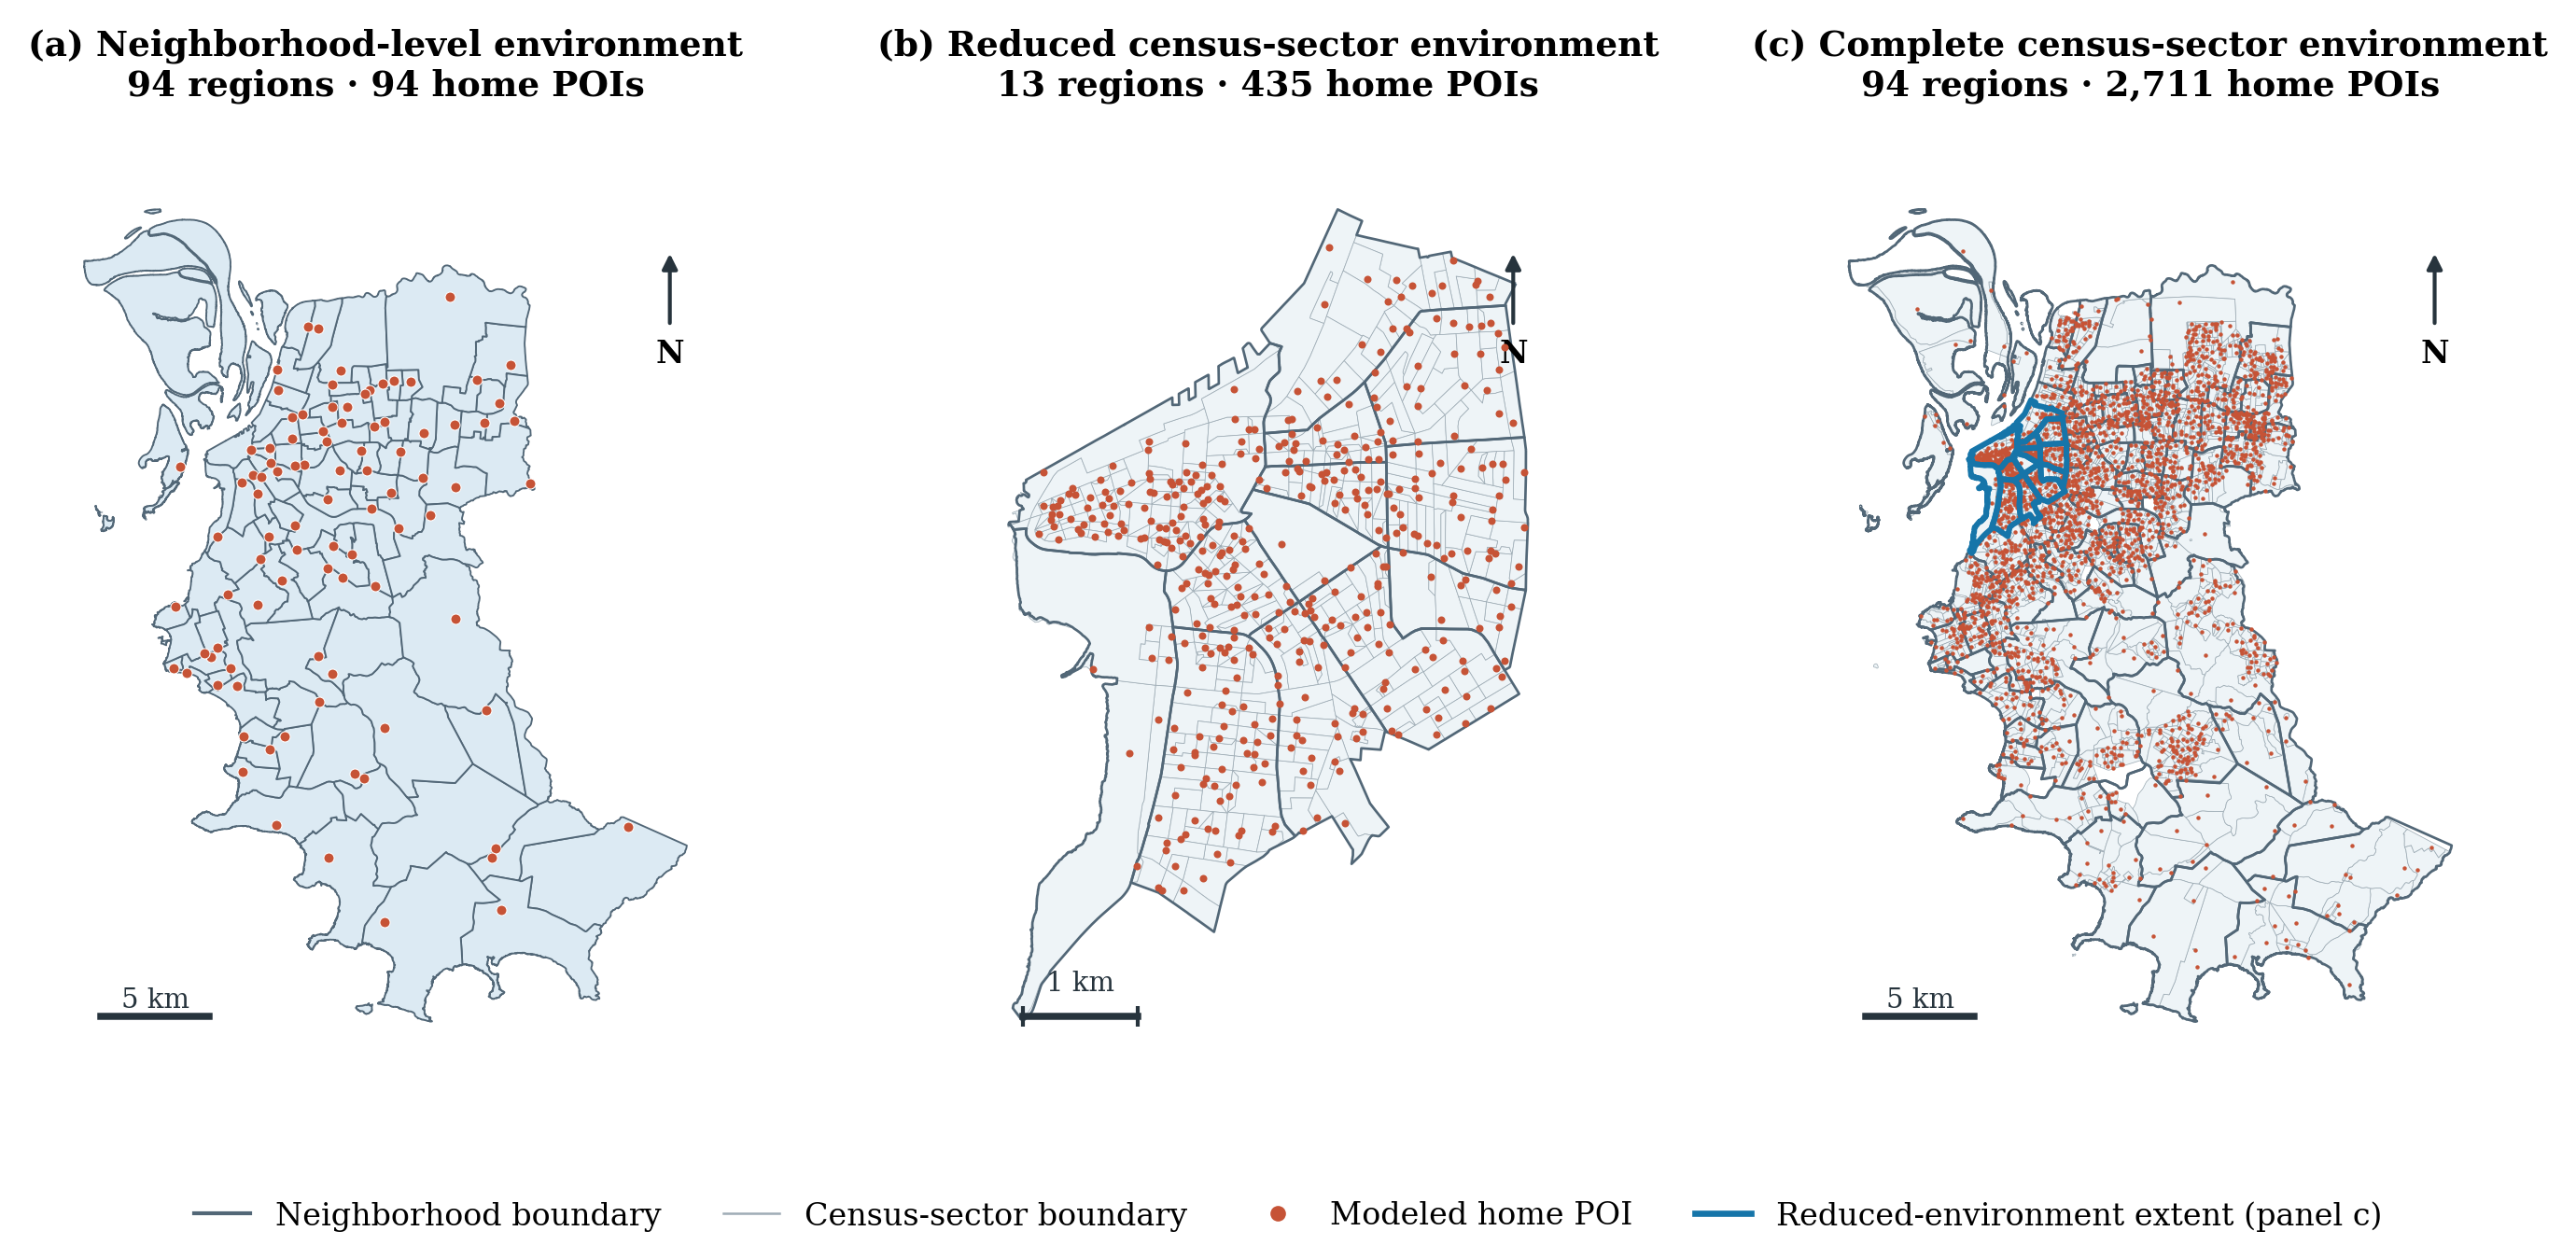
\includegraphics[width=0.99\textwidth]{fig/viz/spatial_environment_comparison.png}
  \caption{Spatial representations of Porto Alegre used in the experiments, highlighting the distribution of home $P$s in the neighborhood-level, reduced census-sector, and complete census-sector environments. The outlines in the complete environment represents the reduced environment’s 13-neighborhoods.}
  \label{fig:spatial_representations}
\end{figure}


\section{Implemented Plugins and Scenario-Specific Inputs}
\label{sec:scenario_specific_inputs}


The spatial representations introduced in the previous section provide the common environment and population basis for the experiments in this thesis. Different application scenarios, however, require additional data and simulation behavior beyond this shared representation. 
These requirements are introduced through domain-specific plugins, which extend the LODUS core model with the state, routines, actions, and simulation-step behavior needed to represent each phenomenon.

This section presents the implemented plugins together with the inputs used to configure and support them. The extensions address normal life mobility, large-scale events, environmental disruptions and shelters, contagion and vaccination, and dialysis services. 
For each case, we describe the role of the plugin, the principal contributions it introduces according to the model defined in Section~\ref{sec:extension_mechanism}, and the external, derived, or scenario-defined inputs required by its behavior. In addition to extending population state and simulation behavior, some plugins also augment the base spatial representations with domain-specific $P$s. 
In the extensions presented here, such additions include shelters, dialysis clinics, and water-treatment facilities. In this way, the section complements the shared environments described above by showing how they are extended and configured for the different experimental scenarios considered in this thesis.
%Table~\ref{tbl:input_plugin_mapping} connects these input families to the extension contract defined in Section~\ref{sec:plugins}. 
%Table~\ref{tbl:input_plugin_mapping} relates these input families to the plugin contributions introduced in Section~\ref{sec:plugins}. The mapping %SO: qual mapping?
%identifies the principal nonempty components used by each experiment family; individual experimental sections report the selected parameter values and policies in greater detail. Environment fields such as $\tau_i$, $\bm{\alpha}_i$, $C_i(t)$, and $D_i$ remain part of the core simulation state even when a plugin declares its conventions or modifies its values. 

\begin{comment}
    
%GA: toda ssa section foi reescrita
%SO: importante na tabela abaixo e em todo texto arrumar aquele "contract"
\begin{table}[ht]
\centering
\footnotesize
\setlength{\tabcolsep}{4pt}
\caption{Principal mapping %SO: correspondence???
from scenario-input families to the plugin extension contract.}
\label{tbl:input_plugin_mapping}
\begin{tabularx}{\linewidth}{@{}p{3.0cm}p{3.4cm}X@{}}
\toprule
\textbf{Experiment family} & \textbf{Principal components} & \textbf{Role of the inputs} \\
\midrule
Routine mobility
& $\bm{\theta}_{\Pi}$, $E_{\Pi}$, $\mathcal{F}_{\Pi}$, $\mathcal{H}_{\Pi}$
& Configures mobility distributions or temporal profiles, declares lifecycle characteristics, and supplies the handlers and step updates that generate and consume movement requests. \\
Large-scale events
& $\bm{\theta}_{\Pi}$, $\mathcal{R}_{\Pi}$, $\mathcal{F}_{\Pi}$
& Defines event times and demand volumes, schedules gathering requests, and consumes them through registered action handlers. \\
Contagion and vaccination
& $\bm{\theta}_{\Pi}$, $E_{\Pi}$, $\mathcal{F}_{\Pi}$, $\mathcal{H}_{\Pi}$
& Defines epidemiological and vaccination parameters, declares population states, and updates those states during execution. \\
Flooding and shelters
& $\bm{\theta}_{\Pi}$, $E_{\Pi}$, $\mathcal{F}_{\Pi}$, $\mathcal{H}_{\Pi}$
& Provides hazard and capacity parameters, declares $P$-attribute conventions and population states, and implements availability and displacement policies. \\
Dialysis services
& $\bm{\theta}_{\Pi}$, $E_{\Pi}$, $\mathcal{F}_{\Pi}$, $\mathcal{H}_{\Pi}$
& Configures recurring demand, clinic schedules and capacity, declares patient states, and implements treatment and return transitions. Clinic dependencies remain represented by $D_i$. \\
\bottomrule
\end{tabularx}
\end{table}
\end{comment}



\subsection{Normal-Life Mobility}
\label{sec:normal_life}

Normal life represents recurring population movements performed under ordinary conditions. These movements are introduced through two complementary mobility plugins: L\'evy Walk and Popular Times. The former generates mobility primarily from stochastic spatial displacement or attendance-based demand, while the latter generates mobility from temporally structured demand profiles associated with different categories of destinations. Together, they provide the baseline population movement upon which other processes, such as large-scale events, epidemic contagion, or environmental disruptions, may operate.

For clarity, the experiments distinguish between two forms of routine movement: \textit{commutes} and \textit{activities}. A \textit{commute} denotes a recurring trip associated with work or school, whereas an \textit{activity} denotes a visit to another urban location, such as a marketplace, restaurant, or pharmacy. These terms characterize the roles assigned to movements in the experiments rather than intrinsic restrictions of the corresponding plugins. 
In the configurations considered in this thesis, L\'evy Walk is primarily used to generate commutes, while Popular Times is used to generate activities. However, either plugin can be configured for other mobility purposes by changing the eligible population, destination types, temporal profiles, and related parameters.


\subsubsection{L\'evy Walk Plugin} 
\label{sec:levy_walk_plugin_inputs}

The \textit{L\'evy Walk Plugin} generates population movement using a stochastic spatial model in which travel distances follow a L\'evy distribution~\cite{levy_flight}. This produces many short-distance movements and progressively fewer long-distance movements, consistent with patterns reported for human mobility~\cite{gonzalez2008understanding}. The plugin does not prescribe a particular semantic purpose for these movements; eligible population groups and destination types are determined through its configuration. 
Rather than reproducing observed individual trajectories, the plugin generates mobility from configurable behavioral parameters, allowing controlled comparisons under different mobility conditions.

The plugin supports two forms of mobility generation. The configuration originally introduced with the published manuscript~\cite{silva2026lodusPop} divides eligible populations into configurable packets and evaluates their movement according to a movement probability. For each moving packet, a travel distance is sampled from the L\'evy distribution and used to select a destination within a corresponding distance interval. The principal inputs of this configuration therefore include the parameters of the L\'evy distribution, movement probability, population-packet size, destination types, and distance discretization. An optional mobility-restriction factor can additionally reduce the population selected for movement when required by a scenario.

For the census-sector environments, the plugin can instead generate demand according to explicit attendance rates. In this configuration, the eligible population expected to commute during a modeled day is determined from configurable attendance parameters and distributed among population origins and departure times according to temporal profiles. Additional configuration parameters determine population-packet limits, destination types, and the duration of each mobility episode.

Population templates determine which groups are eligible for each movement. In the commute configurations considered in this thesis, occupation and age characteristics are used to identify workers and students, while \textit{work} and \textit{school} $P$s provide their respective destinations. These associations are configuration choices and may be changed when the plugin is applied to other forms of mobility.

The attendance-based configuration additionally extends the population representation with traceable characteristics that preserve information about the movement lifecycle, including the original home, requested and receiving destinations, departure time, and scheduled return. These characteristics remain associated with population blobs as they are split, moved, and subsequently returned and merged, allowing requested, completed, and unmet movements to remain distinguishable during simulation execution.

%The specific L\'evy Walk parameters, temporal profiles, population groups, packet sizes, movement durations, and other configuration values adopted by each experiment are presented in the corresponding simulation setup.

\subsubsection{Popular Times Plugin}
\label{sec:popular_times_plugin_inputs}

The \textit{Popular Times Plugin} generates population movement according to temporal demand profiles associated with categories of $P$s. Rather than determining demand primarily from stochastic travel distances, the plugin represents how demand for a destination type varies according to the day of the week and hour of the day. As with L\'evy Walk, the mechanism is not restricted to a particular semantic category of movement: its profiles and destination types may represent commercial activities, services, work, school, or other recurring mobility patterns.

In this thesis, weekly hourly profiles were prepared for marketplaces, restaurants, and pharmacies. These profiles were constructed from temporal patterns observed in the Popular Times feature of Google Maps and describe the relative variation in demand throughout the week. They should therefore be interpreted as temporal demand profiles rather than measured visitation counts for individual establishments.

For each configured destination type, positive hourly profile values are normalized over the week and combined with a configurable visit rate and the population associated with the corresponding demand source. This determines the aggregate number of visits to be generated over the modeled period and their temporal distribution.

When a movement request is processed, the plugin selects eligible population from candidate origins according to the available population and the configured spatial-selection policy. Selected populations are moved to the requested destination and subsequently returned after a configurable visit duration. Through its model extensions, the plugin preserves information such as the population source, requested and receiving destinations, and scheduled return, maintaining the activity lifecycle while the corresponding population is away from its origin.

The temporal profiles constitute input data shared by the Popular Times experiments, whereas visit rates, movement durations, enabled destination types, and other configuration choices determine how these profiles are instantiated in a particular simulation.

The L\'evy Walk and Popular Times plugins can be used independently or composed within the same simulation. Because both operate on the same represented population, their configuration and execution order determine how their respective mobility demands interact. The particular parameter values, destination types, temporal configuration, and execution order adopted in each experiment are therefore defined as part of its simulation setup.


\subsection{Exceptional Events and Environmental Disruptions} 
\label{sec:events_environmental_disruptions}

While the normal-life extensions represent recurring population mobility, other scenarios require temporary changes in demand or in the conditions under which this mobility occurs. In this work, two such cases are considered: (i) large-scale events, which introduce exceptional demand for movement toward specific locations and times; and (ii) environmental disruptions, which modify the availability of locations and may suppress, redirect, or generate new population movements.

Large-scale events introduce temporary demand for movement toward a configured destination without modifying the underlying state of the environment. Environmental disruptions instead modify the availability of affected $P$s, while the response to this change remains determined by the plugin responsible for the corresponding population movement. 
Consequently, the same environmental condition may suppress a movement, redirect it to another destination, or generate new movement toward a shelter. %The following subsections describe the plugins and input data used to represent these mechanisms. The specific configurations adopted by each experiment are presented later with their respective simulation setups.

%GA: troquei o nome de large-scale events para Gather Population. É o nome do plugin mesmo, e ele não é limitado apenas a grandes eventos (qualquer quantidade e qualquer frequencia).
\subsubsection{Gather-Population Plugin} \label{sec:gather_population_plugin_inputs}

Large-scale events are represented through scheduled gathering requests interpreted by the \textit{Gather-Population Plugin}. An event is characterized by configurable information such as its execution time, destination $P$, requested attendance, and the policy used to distribute this demand among potential population origins.

When a gathering request is processed, the plugin identifies eligible population across candidate $P$s and distributes the requested demand among these origins. Origin contributions may be weighted according to their distance from the destination, allowing nearby population to contribute more strongly to the gathering demand. The resulting assignments are translated into \textit{move population} actions (described in Section~\ref{sec:routines}) towards the event destination.

The requested attendance represents demand rather than guaranteed participation. Its fulfillment depends on the eligible population available when the request is processed. This distinction is particularly relevant when gathering requests coexist with normal-life mobility or with other events, since the population distribution may already have been modified by previously executed actions.

Multiple gathering requests can be scheduled independently and may therefore occur at the same or at different simulation steps. Requests executed at the same step are processed sequentially, so each one operates on the population state produced by those processed before it. %The event destinations, requested attendance values, execution times, and combinations considered in the experiments are specified in their corresponding simulation setup.



\subsubsection{Water-Level Data Plugin}
\label{sec:water_level_plugin_inputs} 

The flood scenarios are motivated by the extreme flooding that affected Porto Alegre and other municipalities in Rio Grande do Sul in 2024. The event caused extensive disruption to urban areas and infrastructure, providing a relevant real-world context for examining how environmental conditions can affect the availability of locations and population mobility.

The \textit{Water-Level Data Plugin} represents these changes in $P$ availability by separating the spatial susceptibility of each location from the environmental condition applied during a simulation.

Flood susceptibility is represented through the $P_i$ attribute $\bm{\alpha}_i[\mathrm{water\_level}]$, which stores a location-specific exposure threshold. This value indicates the minimum water level at which the corresponding $P$ is considered flooded and should not be interpreted as the water level currently applied to the simulation. 

For the environments used in this thesis, these thresholds were derived from the simulated ``Water Level'' map provided by Climate Central's Coastal Risk Screening Tool\footnote{Climate Central Coastal Risk Screening Tool: \url{https://coastal.climatecentral.org/map}.}. The coordinates of modeled $P$s were evaluated at successive water levels, and the minimum level at which each location was represented as inundated was assigned as its exposure threshold. 
The resulting $P$ attributes contain exposure thresholds ranging from 3.0~m to 10.0~m, providing a reusable spatial representation of flood susceptibility independently of the water-level condition selected for an experiment.

Figure~\ref{fig:flood_exposure_thresholds} shows the spatial distribution of these exposure thresholds in the reduced and complete census-sector environments. The figure represents the values stored in $\bm{\alpha}_i[\mathrm{water\_level}]$ and therefore characterizes the environmental input rather than the availability state produced during a particular simulation.

\begin{figure}[ht] 
    \centering 
    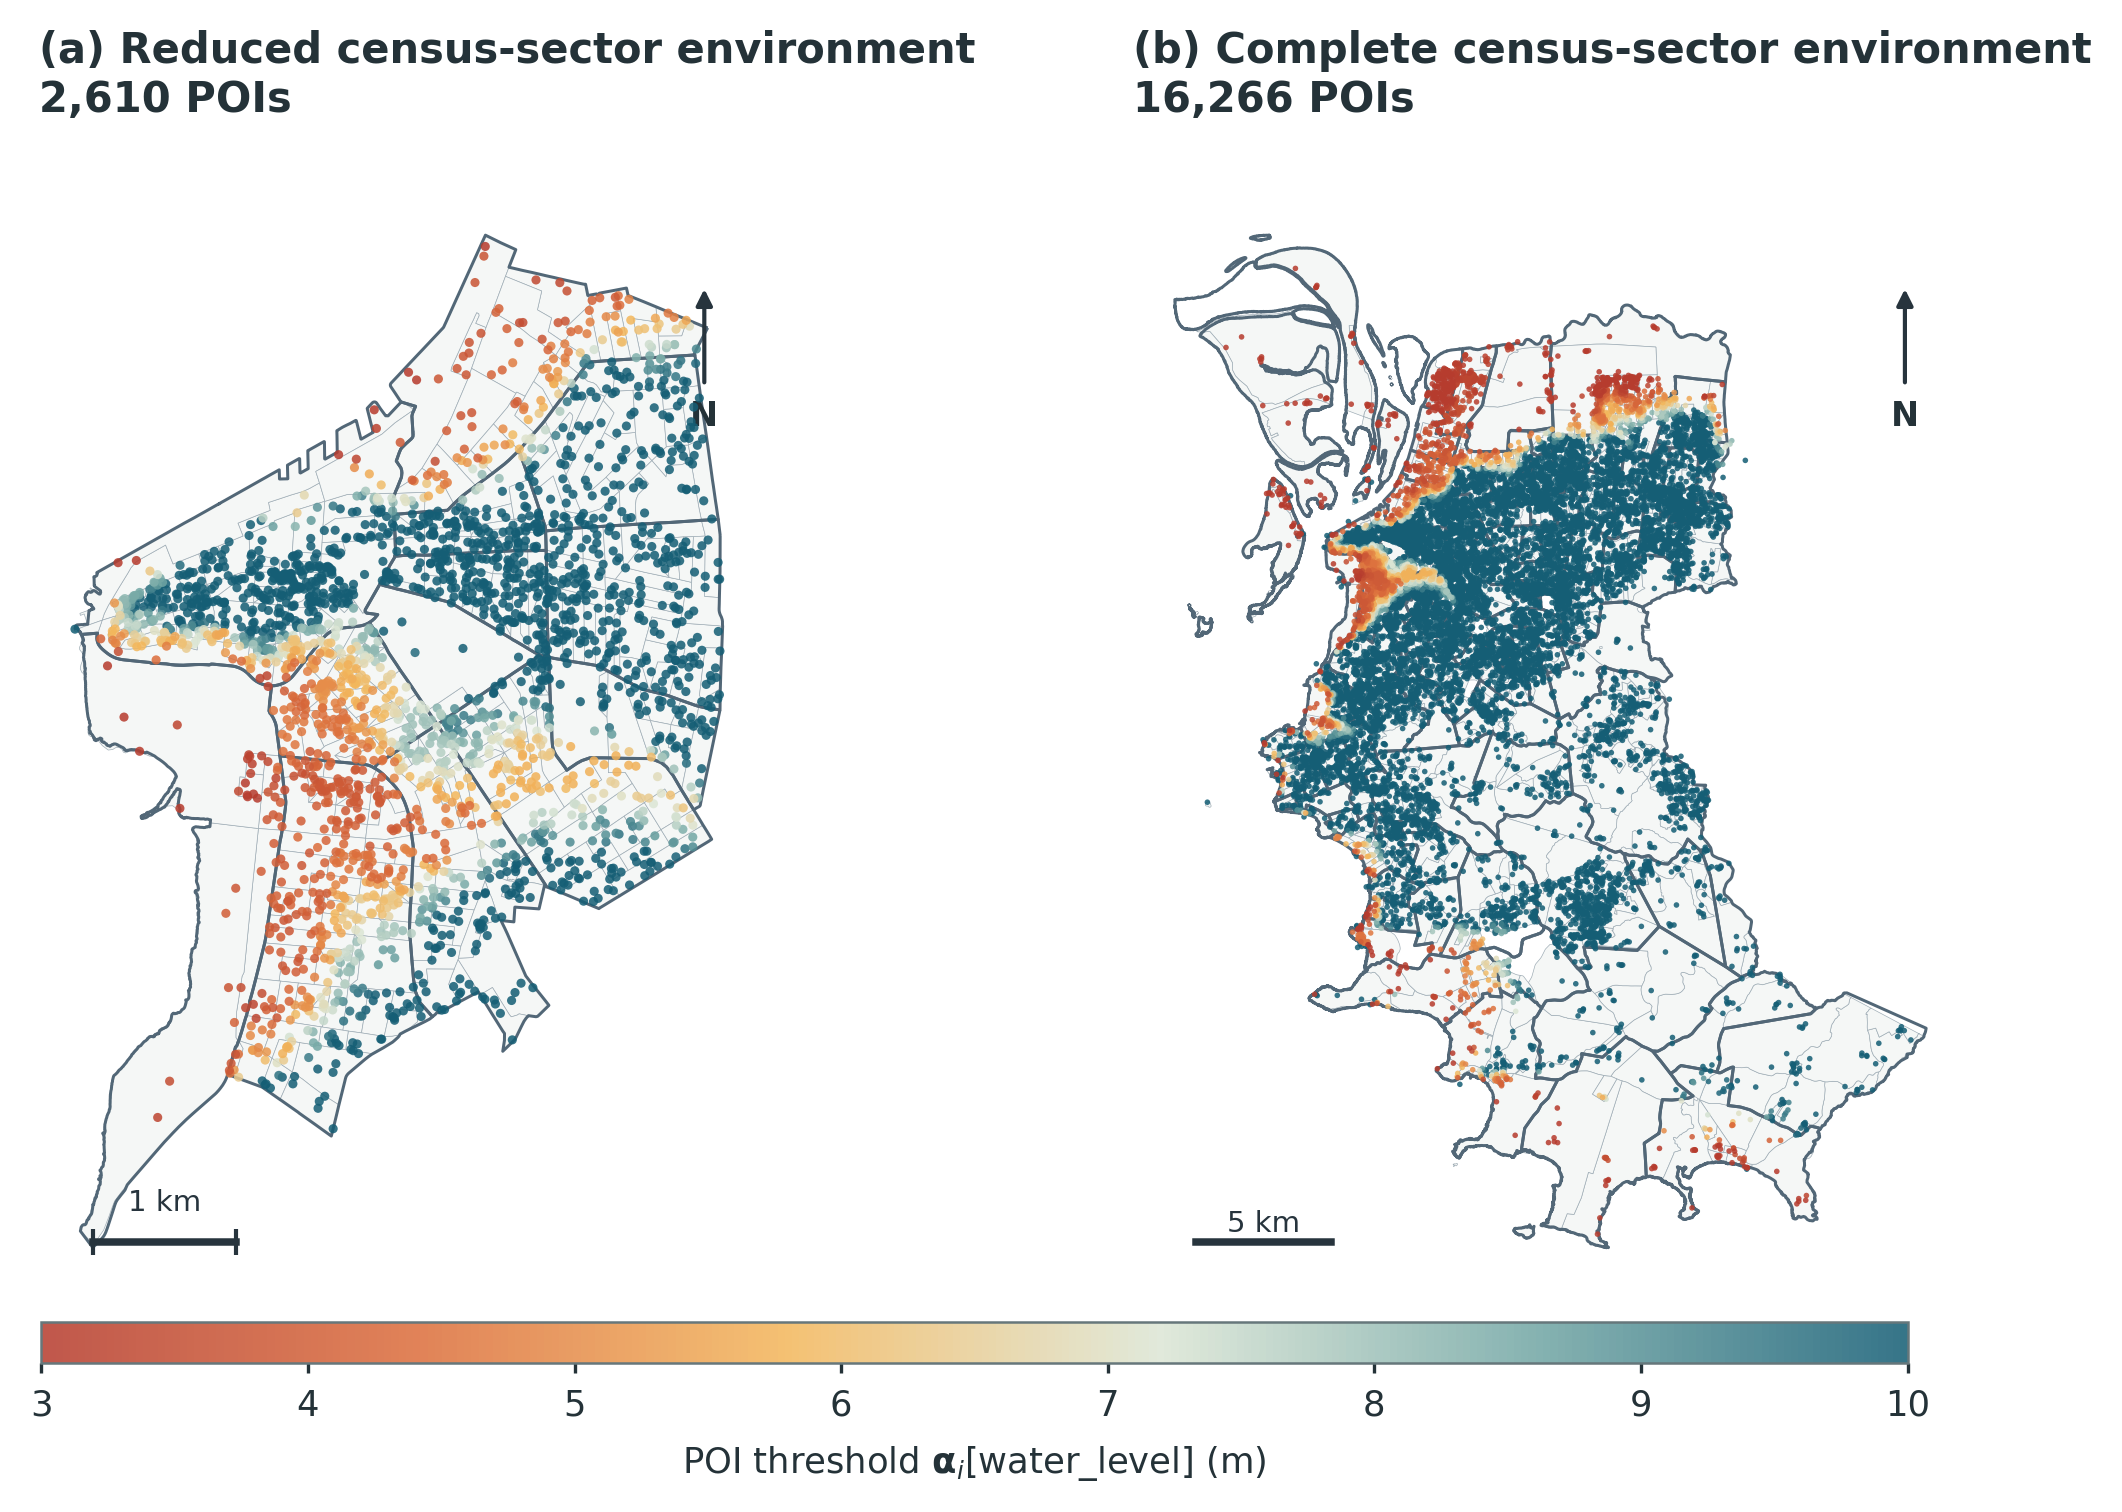
\includegraphics[width=0.99\textwidth]{fig/viz/flood_exposure_thresholds_comparison.png} 
    \caption{Spatial distribution of $P$ flood-exposure thresholds in the (a) reduced and (b) complete census-sector environments. Marker color represents $\bm{\alpha}_i[\mathrm{water\_level}]$, the minimum modeled water level at which the corresponding $P$ is treated as flooded.} 
    \label{fig:flood_exposure_thresholds} 
\end{figure}

The current water-level condition is supplied separately through the plugin configuration and may be represented by a static value or a time-varying sequence. The flood-aware mobility experiments use historical observations obtained from a public water-level dashboard\footnote{Historical water-level dashboard: \url{https://bit.ly/4wIpZPC}.}. These observations were processed into an hourly sequence compatible with the simulation time steps. Other configurations may instead use synthetic water-level values when controlled disruption conditions are required.

At each simulation step, the plugin compares the current water level with the exposure threshold of each configured $P$. When the current value reaches or exceeds the threshold, a direct disabling condition \textit{flood} is added to $C_i(t)$. When the level falls below the threshold, only this condition is removed. A $P$ therefore remains unavailable if another direct condition or an unsatisfied dependency continues to prevent its operation.

The Water-Level Data Plugin changes the state of the environment but does not itself determine how the population responds to that state. Movement suppression, destination substitution, evacuation, or other responses remain responsibilities of the plugins that execute actions involving the affected locations.


%GA: posso combinar com o texto inicial, mas pensei em deixar aqui após comentar a ideia de availability e de desabilitar Ps. E destacar que tem opções distintas de configurações
\subsubsection{Popular Times and L\'evy Walk Plugins: Mobility Policies under $P$ Unavailability} 
\label{sec:availability_aware_mobility_plugins} 

The Popular Times and L\'evy Walk plugins described in Section~\ref{sec:normal_life} can account for $P$ availability when processing normal-life movement. This allows environmental disruptions to affect recurring mobility.

The \textit{Popular Times Plugin} can suppress an activity request when its origin or requested destination is unavailable. It also provides an optional destination-substitution policy in which an unavailable destination is replaced by an available $P$ of the same type. In this case, the plugin retains both the requested and receiving destinations, allowing redirected demand to remain distinguishable from demand originally associated with the alternative location. 

The \textit{L\'evy Walk Plugin} can likewise account for unavailable origins and destinations. In the attendance-based configuration used for work and school mobility, requests that cannot be completed because of $P$ availability are retained as unmet demand.
The plugin records the information required to distinguish requested, fulfilled, and interrupted mobility and to preserve the original home associated with the population.

These responses are configuration and policy choices rather than intrinsic semantic restrictions of the mobility plugins. For example, the experiments in this thesis allow substitution for selected activity destinations while treating unavailable work and school destinations as unmet commute demand. Other simulations may configure different destination types or response policies according to their modeling objectives. %This separation between environmental state and mobility response allows the same flood condition to be combined with different assumptions about how populations adapt to unavailable locations.


\subsubsection{Shelter Plugin} \label{sec:shelter_plugin_inputs} 

The \textit{Shelter Plugin} represents evacuation and temporary accommodation of populations affected by an environmental disruption. In contrast to mobility suppression or destination substitution, sheltering introduces new movement in response to population exposure. The plugin combines information about exposed populations with the locations, capacities, occupancies, and availability of shelter $P$s. 

Shelter information was collected from the Abrigos RS website on May 15, 2024\footnote{Abrigos RS: \url{https://abrigosrs.org/}.}. The collected dataset contained 128 records with names, addresses, coordinates, neighborhoods, capacities, occupancies, and free-text observations. After filtering incomplete records, the Shelter Plugin adds 104 $P$s of type \textit{shelter} to the selected base environment, with a combined recorded capacity of 12,519 people and an initial occupancy of 10,963. These shelter $P$s are therefore not part of the shared spatial representations described in Section~\ref{sec:spatial_representations}; they are introduced only when the Shelter Plugin is included in a simulation.

Figure~\ref{fig:shelter_locations_status} presents the spatial distribution and reported initial occupancy of the shelters added to the environment. In addition to illustrating the domain-specific $P$s introduced by the Shelter Plugin, the map shows the uneven spatial distribution of shelter capacity across Porto Alegre.

\begin{figure}[ht]
\centering
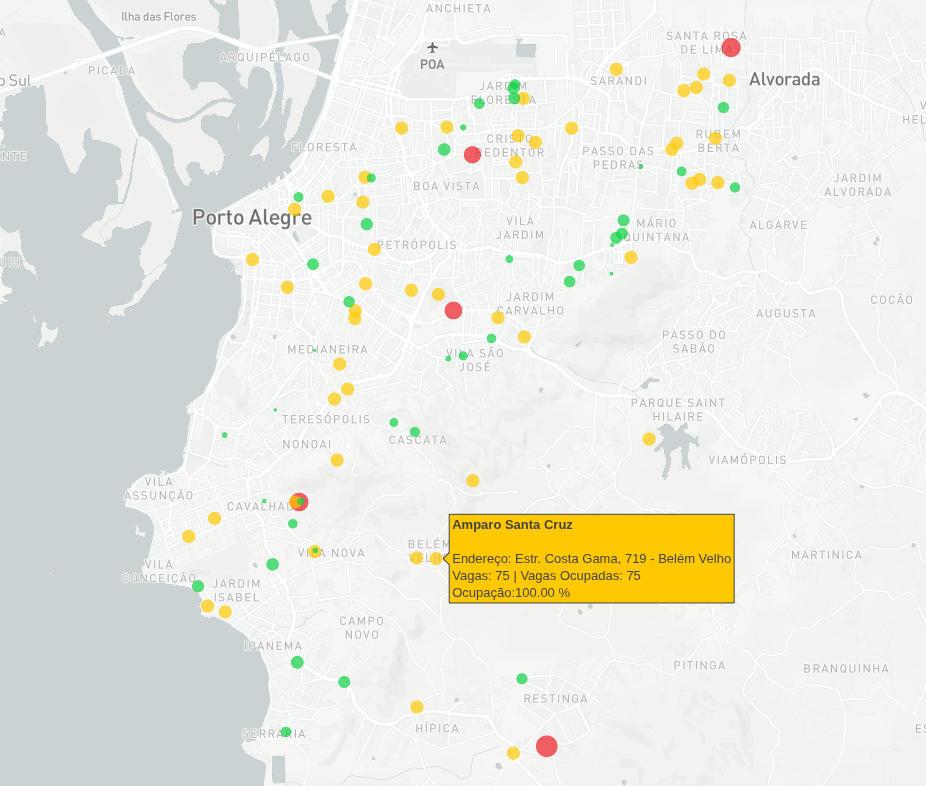
\includegraphics[width=0.85\textwidth]{fig/viz/shelters.png}
\caption{Shelter locations and reported initial occupancy in Porto Alegre. Marker color distinguishes shelters with available capacity, shelters at capacity, and shelters whose recorded occupancy exceeds their reported capacity; marker size is proportional to capacity.}
\label{fig:shelter_locations_status}
\end{figure}

Shelter coordinates, capacities, occupancies, and other facility-specific information are represented through attributes in $\bm{\alpha}_i$. Population exposure is defined separately and can therefore be configured independently from the shelter network and its available capacity. 

The plugin introduces the traceable characteristic \texttt{flooding\_status}, used to distinguish populations classified as \texttt{safe}, \texttt{in\_danger}, or \texttt{sheltered}. Because this state remains associated with population blobs, exposed, waiting, and admitted populations can coexist at the same $P$ without losing their respective conditions. 

The \textit{Shelter Plugin} comprises three principal behaviors. 
First, eligible populations in danger may be requested to move toward available shelter according to a configured evacuation policy. 
Second, populations arriving at a shelter are admitted according to its remaining capacity; those that cannot be accommodated remain in the \texttt{in\_danger} state. 
Third, an optional reallocation mechanism can transfer waiting populations from a full or unavailable shelter to other available facilities with remaining capacity. 

Shelter capacity and $P$ availability are represented separately. A shelter reaching its capacity is not automatically considered unavailable; instead, additional admission is rejected by the shelter policy. Conversely, a shelter may become unavailable because of an independent condition, such as a configured facility failure, represented through its cause set $C_i(t)$. This distinction allows service capacity, environmental conditions, and facility failures to be combined without treating them as equivalent properties of the environment.

%The plugin can be configured with parameters controlling population exposure, evacuation response, capacity, reallocation, and facility availability. 
%The particular exposure conditions, response rates, capacity variations, failure configurations, execution schedule, and other experimental choices are defined later in the corresponding simulation setup.


\subsection{Health-Related Processes and Services}
\label{sec:health_processes_services}

The preceding extensions primarily introduce or modify population movement. Health-related scenarios additionally require changes in population state and access to recurring services. In this work, these requirements are represented through plugins for epidemic contagion, vaccination, and dialysis treatment, together with mechanisms for representing dependencies between healthcare facilities and supporting urban infrastructure.

The epidemic plugins operate directly on the population represented at each $P$, allowing health states to evolve as different population groups share locations over time. The dialysis plugin instead introduces recurring treatment demand and selects among available service locations according to their schedules, capacities, and infrastructure dependencies. 
Although these applications address different processes, both illustrate how domain-specific state and behavior can be added without modifying the general definitions of population blobs, $P$s, or regions. The specific epidemiological parameters, vaccination configurations, treatment demand, service capacities, and disruption scenarios adopted in the experiments are presented later in their respective simulation setups.

\subsubsection{Infection Plugin}
\label{sec:infection_plugin_inputs}

The \textit{Infection Plugin} represents epidemic contagion using a susceptible--infected--removed (SIR) model~\cite{kermack1927contribution}. Through its model extension, the plugin introduces a traceable characteristic representing the SIR state, with the possible values \texttt{susceptible}, \texttt{infected}, and \texttt{removed}. The removed state indicates that a population no longer participates in contagion and does not distinguish recovery, immunity, and mortality as separate outcomes.

Because the SIR state is traceable, populations with different epidemiological states remain distinct when they occupy the same $P$. At each contagion update, the plugin evaluates the susceptible and infected populations currently co-located at a $P$. For a total population $N$, the implemented dynamics follow

\begin{equation}
   \frac{dS}{dt}=-\frac{\beta I S}{N},
\end{equation}

\begin{equation}
   \frac{dI}{dt}=\frac{\beta I S}{N}-\gamma I,
\end{equation}

\begin{equation}
   \frac{dR}{dt}=\gamma I,
\end{equation}

where $S$, $I$, and $R$ denote the susceptible, infected, and removed populations, respectively, while $\beta$ and $\gamma$ represent the infection and removal rates. The corresponding basic reproduction number is given by $R_0=\beta/\gamma$.

The plugin configuration specifies the epidemiological parameters and the initial infected population. Since contagion is evaluated during simulation execution, population movement changes which groups share a $P$ and consequently which populations participate in each local infection update. Fractional transitions resulting from the aggregate SIR calculations are retained between evaluations and subsequently converted into integer population quantities while preserving the represented population.

The Infection Plugin can also access information supplied by other plugins. In the vaccination experiments, vaccine effectiveness modifies the susceptible-to-infected transition according to the vaccination state of the population. %The particular initialization, epidemiological parameters, execution frequency, and mobility conditions used in each experiment are specified in the corresponding simulation setup.

\subsubsection{Vaccination Plugin}
\label{sec:vaccination_plugin_inputs}

The \textit{Vaccination Plugin} represents the allocation of vaccine doses and the progressive vaccination state of the population. It introduces the traceable characteristic \texttt{vaccine\_level}, whose value records the vaccination level attained by each population blob. Because this characteristic is preserved during movement and blob operations, populations with different vaccination states can remain distinguishable throughout the simulation.

The plugin configuration defines the number of vaccination levels (i.e. doses), the effectiveness associated with each level, the conditions under which subsequent doses become available, and the temporal series of available doses to be applied. When a vaccination request is processed, eligible population is selected, its vaccination level is updated, and the resulting state remains associated with that population after it returns to its previous location.

The vaccination quantities used in this thesis are based on the daily Porto Alegre series obtained from the Rio Grande do Sul vaccination dashboard\footnote{Rio Grande do Sul COVID-19 vaccination dashboard: \url{https://vacina.saude.rs.gov.br/}.}. The source reports doses applied by date and provides an observed temporal input. In the simulations, the distribution of these quantities among the modeled population is controlled by the vaccination plugin and its scenario configuration.

Additionally, vaccination state can be accessed by extensions. In the epidemic experiments, the Infection Plugin uses the effectiveness associated with the current vaccination level to modify modeled susceptibility. %The effectiveness values, dose schedules, allocation policy, and other experimental choices are defined in the corresponding simulation setup.

\subsubsection{Dialysis Plugin}
\label{sec:dialysis_plugin_inputs}

The \textit{Dialysis Plugin} represents access to recurring, capacity-constrained treatment. Unlike occasional service demand, dialysis requires patients to return periodically for treatment, so temporary limitations in clinic availability or capacity may produce demand that remains unresolved after the original treatment time. 

The infrastructure required by the dialysis experiments is not part of the base census-sector environments. When the dialysis-related extensions are loaded, domain-specific $P$s representing dialysis clinics and supporting water-treatment facilities are added to the selected spatial representation.

The plugin configuration defines the population requiring treatment, the interval between treatments, the $P$ types representing patient origins and dialysis clinics, and the service schedules and treatment capacities associated with the clinics. Default schedule and capacity values can be provided for the clinic type, while clinic-specific configurations allow individual facilities to use different operating intervals or capacities without changing the treatment mechanism. 
%The clinic schedules and treatment capacities used in the experiments are scenario-defined parameters rather than observed estimates of service operation.

The plugin extends the population representation with traceable characteristics required to preserve the treatment lifecycle. These include whether a population requires dialysis, its treatment frequency, next due date, current treatment status, residence origin, and treatment progression. Initial due dates may be distributed across the treatment interval so that recurring demand does not necessarily occur simultaneously for the entire patient population.

During simulation execution, the plugin identifies patients whose treatment is due and searches for an eligible clinic. Clinic eligibility combines several conditions: the facility must be available according to $C_i(t)$ and $D_i$, it must be operating at the current simulation step, and it must have remaining treatment capacity. Among eligible facilities, the extension selects a geographically suitable clinic and moves the corresponding population for treatment. After treatment is completed, patients return to their origin, while patients who cannot be admitted remain due and may be reconsidered during subsequent simulation steps.

These conditions distinguish service operation from $P$ availability. A clinic outside its opening interval or with exhausted treatment capacity remains an available $P$ but cannot accept additional treatment at that time. A clinic affected by a direct unavailability condition or an unsatisfied infrastructure dependency, in contrast, is unavailable to the treatment action.

\subsubsection{Dependency-Mapping Plugin}
\label{sec:dependency_mapping_plugin_inputs}

Dialysis services are also used to exercise the dependency component $D_i$ of each $P_i$. The \textit{Dependency-Mapping Plugin} constructs relationships between service $P$s and the infrastructure required for their operation. In our experiments, dialysis clinics depend on water-treatment facilities, represented as $P$s of type \textit{water source}.

The resulting infrastructure overlay contains dialysis clinics and water-treatment stations (\textit{Estações de Tratamento de Água}, ETAs), represented as additional $P$s of type \textit{dialysis clinic} and \textit{water source}, respectively. ETA locations and the association of neighborhoods with water-supply systems were derived from information published by the Municipal Department of Water and Sewage (DMAE)\footnote{DMAE water-system information: \url{https://prefeitura.poa.br/dmae/informacoes-agua}.}. The complete overlay contains six water-treatment stations and 12 dialysis clinics.

Figure~\ref{fig:dialysis_network} illustrates the dialysis infrastructure represented in the environment and the relationships between clinics and their supporting water sources. The clinic-centered view identifies the water sources on which a selected clinic depends, while the water-source-centered view highlights the neighborhoods supplied by a selected source. 

\begin{figure}[!ht]
    \centering

    \begin{subfigure}{\linewidth}
        \centering
        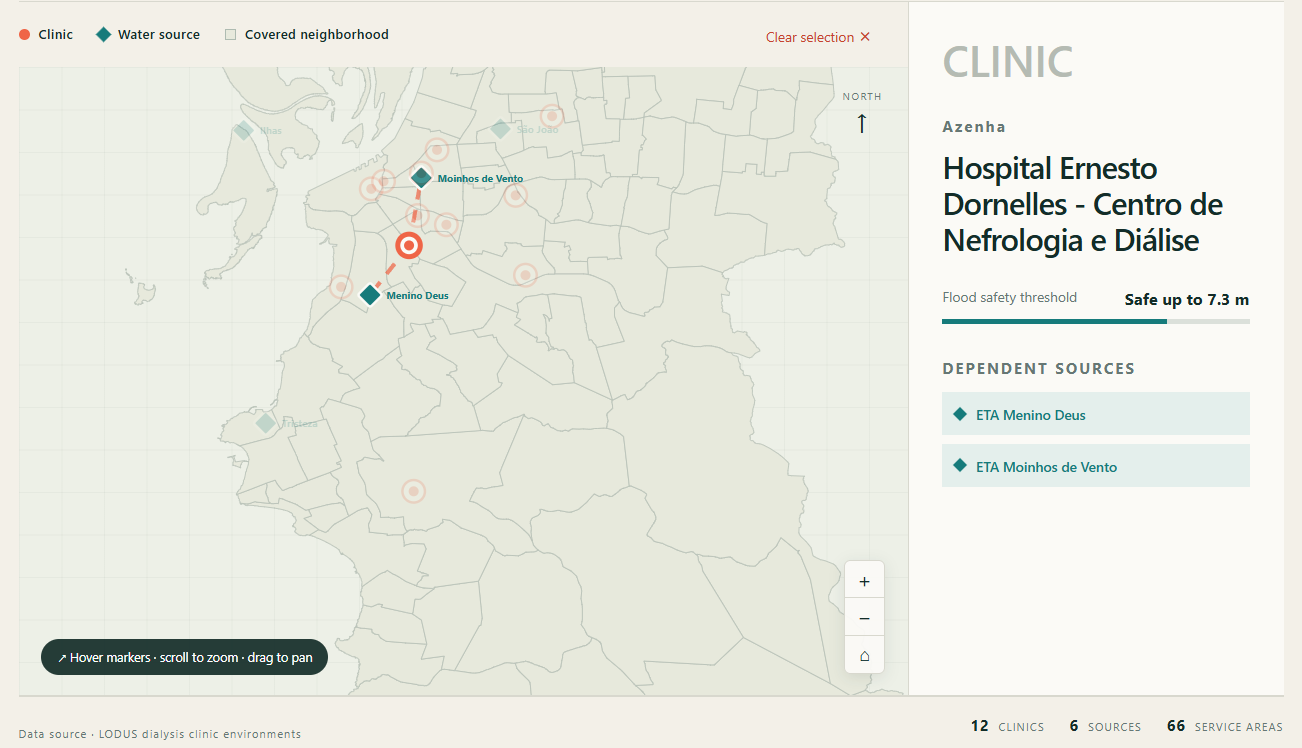
\includegraphics[width=\linewidth]{fig/viz/dialysis_viz_clinic.png}
        \caption{Clinic-centered view showing the water sources supporting a selected dialysis clinic.}
        \label{fig:dialysis_network_clinic}
    \end{subfigure}

    \vspace{0.5em}

    \begin{subfigure}{\linewidth}
        \centering
        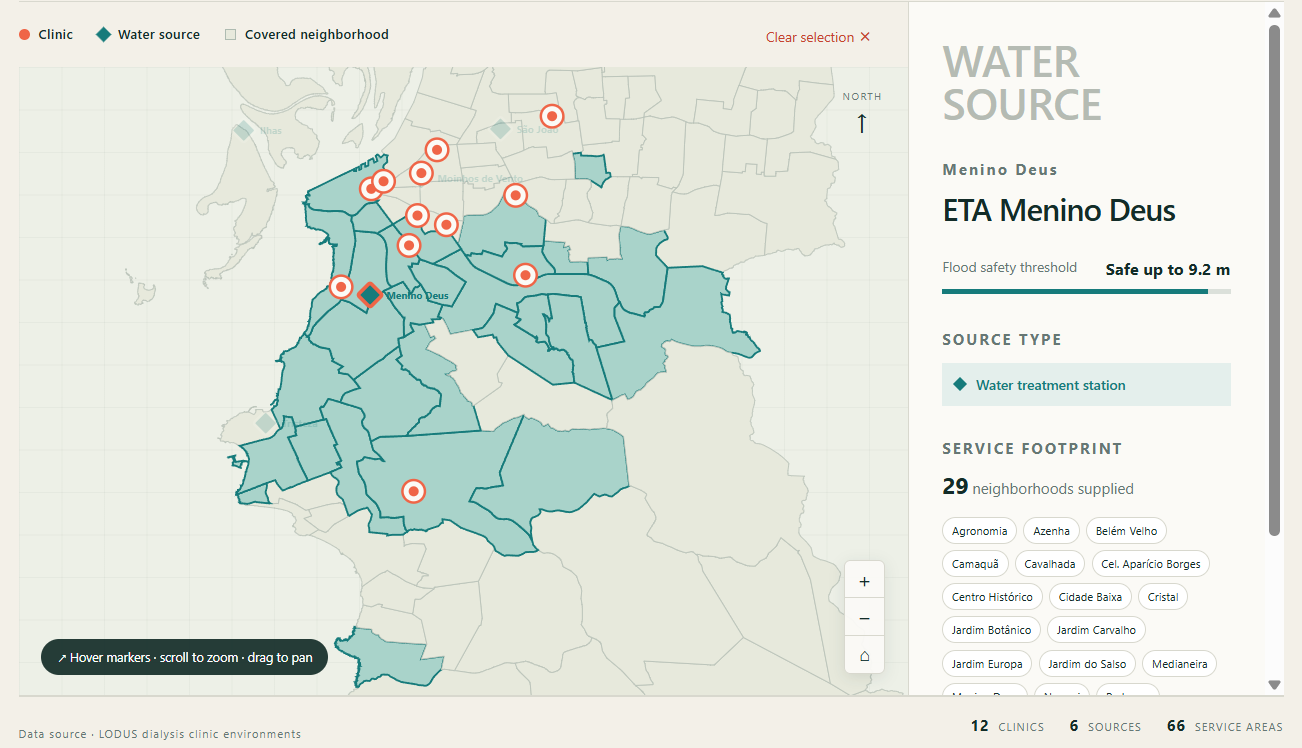
\includegraphics[width=\linewidth]{fig/viz/dialysis_viz_eta.png}
        \caption{Water-source-centered view showing the neighborhoods supplied by a selected water source.}
        \label{fig:dialysis_network_source}
    \end{subfigure}

    \caption{Visualization of the dialysis infrastructure represented in the Porto Alegre environment. 
    (a) Selecting a dialysis clinic identifies its supporting water sources, illustrating the relationships represented by its dependency rules \(D_i\). 
    (b) Selecting a water source highlights its service footprint across the environment.}
    \label{fig:dialysis_network}
\end{figure}

Dialysis clinic locations and their relations to water sources were defined as inputs to the health-service representation. Names, coordinates, external identifiers, and the identifiers used to associate clinics with water sources are stored in the attribute mapping $\bm{\alpha}_i$ of each corresponding $P_i$.

The plugin interprets these attributes when the environment is initialized and constructs the associated dependency rules in $D_i$. The dependency configuration determines which $P$ types act as dependent facilities and supporting resources, how they are matched, and how many supporting $P$s must remain available for the dependency to be satisfied. The generic environment mechanism subsequently evaluates these rules, so the plugin is responsible for constructing the relationships rather than implementing a dialysis-specific availability mechanism.

As a result, a direct disruption to a water-source $P$ may indirectly make one or more dialysis clinics unavailable without adding the same direct cause to those clinics. This separation allows the dependency structure to be reused with different disruption mechanisms.

\subsubsection{Scheduled-Availability Plugin}
\label{sec:scheduled_availability_plugin_inputs}

The \textit{Scheduled-Availability Plugin} provides a generic mechanism for changing $P$ availability at configured simulation steps. It schedules actions that add or remove a named direct disabling condition from the cause set $C_i(t)$ of the corresponding $P_i$, allowing temporary or persistent facility outages to be represented independently of the service-specific plugins that use those locations.

In the dialysis scenarios, this mechanism is used to represent controlled outages of water sources or clinics through the direct condition \texttt{off\_cycle}. Because individual conditions are stored independently in $C_i(t)$, removing a scheduled-outage condition does not restore a $P$ when another condition remains active. Similarly, restoring a water source only restores dependent clinics when their dependency rules in $D_i$ become satisfied and the clinics have no remaining direct disabling condition.

The Scheduled-Availability Plugin can therefore be composed with the Water-Level Data Plugin introduced in Section~\ref{sec:water_level_plugin_inputs}. Flooding and scheduled outages remain distinct direct conditions, while infrastructure dependencies propagate the resulting availability state to dependent facilities. %The particular outage locations, execution times, recovery conditions, and combinations with flooding used in the dialysis experiments are specified in their simulation setup.




\section{Input Provenance and Interpretation}
\label{sec:input_provenance_summary}

Because the experiments combine externally sourced data, derived spatial attributes, and scenario-defined parameters, their provenance must be considered when interpreting the results. This distinction is particularly important when experimental inputs are used to test model behavior rather than to reproduce observed conditions in Porto Alegre.
Table~\ref{tbl:simulation_data_provenance} summarizes the role and sources of the principal data families in the same general order in which they are introduced above.

\begin{table}[ht]
\centering
\footnotesize
\setlength{\tabcolsep}{4pt}
\caption{Provenance and interpretive status of the principal environment and scenario-input families.}
\label{tbl:simulation_data_provenance}
\begin{tabularx}{\linewidth}{@{}p{3.5cm}p{6.2cm}X@{}}
\toprule
\textbf{Data family} & \textbf{Documented basis} & \textbf{Interpretive status} \\
\midrule

Neighborhood geometry and $P$s
& City Hall boundaries and OpenStreetMap amenities
& Externally sourced spatial data used to construct the neighborhood-level environment. \\

Neighborhood population
& IBGE, ObservaPOA, and PROCEMPA
& Externally sourced demographic data used to initialize the population represented in each neighborhood. \\

Census-sector environments
& IBGE 2022 geometries and aggregates
& Official census data spatially processed to construct the finer-grained population and $P$ representation. \\

L\'evy Walk parameters
& Scenario-defined behavioral and routine parameters
& They support controlled mobility comparisons and are not calibrated estimates of observed Porto Alegre trajectories. \\

Popular Times profiles
& Type-specific temporal profiles derived from patterns observed in Google Maps Popular Times
& Derived temporal-demand profiles rather than measured visitation counts for individual establishments. \\

Large-scale event inputs
& Existing modeled event locations with scenario-defined event times and attendee requests
& The request of 500,000 attendees per event is a stress parameter rather than an observed attendance value. \\

Contagion parameters
& Reported $R_0$ values from studies of COVID-19 transmission in Brazil; remaining epidemic and restriction parameters configured by scenario
& The experiments provide controlled comparisons rather than calibrated epidemiological forecasts. \\

Vaccination quantities
& Applied-dose series from the Rio Grande do Sul vaccination dashboard
& Observed daily vaccination quantities; doses are distributed among modeled regions in proportion to their populations.\\

Flood thresholds and exposure
& Climate Central simulated water-level map evaluated at the coordinates of modeled $P$s
& Derived exposure attributes representing the minimum modeled water level at which each location becomes inundated.\\

Water-level
& Public Power BI records from May--June 2024 plus synthetic stress sequences
& Historical observations are used for flood-mobility scenarios, while synthetic sequences are used for controlled stress experiments.\\

Shelters
& Abrigos RS snapshot collected on May 15, 2024
& Historical snapshot of shelter locations, capacities, and occupancies; the original source is no longer available online. \\

ETAs and dialysis clinics
& DMAE water-system information; clinic data and dependency definitions
& Infrastructure locations and dependencies provide the scenario topology, while clinic schedules and hourly treatment capacities are synthetic experimental parameters. \\
\bottomrule
\end{tabularx}
\end{table}

%SO: re-escrevi e tirei o uncertanty porque acho que merece uma discussao nas finals
%Across the following results, externally sourced coordinates, population quantities, and capacities provide geographic and operational context, while behavioral parameters, demand volumes, failures, environmental conditions, and policy responses define the comparisons being tested. Consequently, uncertainty in the source data and uncertainty due to stochastic simulation represent different aspects of the experiments.
Across the experiments presented in the following chapter, externally sourced data provide the spatial, demographic, and service context of Porto Alegre, while scenario-specific parameters define the mobility patterns, disruptions, demands, and responses to be evaluated. This distinction allows the same underlying environments to support different experimental conditions and provides a common basis for interpreting the simulation results.




    

\begin{comment}
    

%SO: re-escrevi abaixo, podes ver comentários na parte comentada. Estava muito com cara de manual; Revisar para validar
\section{OLD:Routine Mobility Inputs}
\label{sec:behavioral_policy_input_data}

Routine mobility provides the baseline movement patterns of the simulated population. These movements represent the daily activities performed by individuals under normal conditions and serve as the basis upon which other processes, such as large-scale events, epidemics, or environmental disruptions, may introduce additional mobility demands. Two complementary mobility models are considered in the core model of this thesis: a stochastic L\'evy Walk model
and a model based on temporal activity profiles derived from Popular Times.

\paragraph{L\'evy Walk:}

The L\'evy Walk model %SO: ref
represents routine mobility through configurable
behavioral parameters rather than observed trajectories. Its objective is to
produce realistic baseline movement patterns while allowing controlled
experiments under different mobility conditions. The input parameters include
the heavy-tailed travel-distance scale, packet size, mobility restriction
factor, worker attendance rate, student attendance rate, departure-hour
profiles, and visit durations.

These parameters configure the mobility model adopted in the core model,
while the corresponding plugin introduces the additional mobility-related
state and behaviors required to represent commuting activities.

\paragraph{Popular Times:}

This thesis proposes a routine mobility model driven by temporal activity
profiles inspired by the Popular Times feature of Google Maps. The model
captures how the demand for different categories of urban activities varies
throughout the week and uses this information to generate routine mobility
patterns. Three weekly hourly profiles are considered, corresponding to
marketplaces, restaurants, and pharmacies. These profiles were constructed
from the temporal activity patterns observed in the Popular Times feature of
Google Maps.

Unlike the stochastic destination selection adopted by the L\'evy Walk model,
the proposed Popular Times model directly represents the temporal demand for
different categories of points of interest. Consequently, the likelihood of
visiting each type of location varies according to the day of the week and
hour of the day, producing routine mobility patterns that better reflect the
temporal dynamics of urban activities.

\paragraph{Large-scale events.}

Large-scale events introduce temporary concentrations of population at
specific locations and times. Each event is characterized by its scheduled
time, destination point of interest, and expected number of participants.
Event locations correspond to existing points of interest in the modeled
environment, while attendance values are defined according to the scenario
being evaluated rather than historical observations.

These inputs define the event scenarios considered in this thesis and are
later interpreted by the event plugin to generate the corresponding
population movements.



%SO: parei aqui

\paragraph{Contagion and vaccination.}
The contagion experiments combine mobility with infection, vaccination, and restriction parameters in the same population representation. Epidemic initialization, homogeneous infection and removal parameters, vaccine-effectiveness values, dose-start days, and restriction levels define comparative scenarios. The three reported $R_0$ values are based on studies of COVID-19 transmission in Brazil~\cite{dutra2020covidR0,deSouza2020covirR0,dutra2021covidR0}, while the daily vaccination quantities follow the 546-value Porto Alegre series obtained from the Rio Grande do Sul vaccination dashboard\footnote{Rio Grande do Sul COVID-19 vaccination dashboard: \url{https://vacina.saude.rs.gov.br/}.}. The dashboard reports doses applied by date, and the simulation distributes the daily Porto Alegre quantities among modeled regions in proportion to their populations.

The epidemiological, restriction, effectiveness, and dose-distribution values form $\bm{\theta}_{\Pi}$. Infection and vaccination states are traceable characteristics declared through $E_{\Pi}$, ensuring that actions can select them through $\bm{T_{Tc}}$ and that blobs with different states remain distinct during merging. Registered handlers and time-step hooks in $\mathcal{F}_{\Pi}$ and $\mathcal{H}_{\Pi}$ implement infection transitions and vaccination updates.

\subsection{Environmental-Disruption Events}

%SO: re-escrevi, valide!
Environmental disruption events illustrate how a hazard can alter the availability of locations, suppress or redirect routine mobility, and create demand for capacity-constrained shelters. The proposed mechanism can accommodate different types of hazards, such as floods or fires, provided that the corresponding spatial exposure and hazard conditions are defined. In the present work, we focus on flood scenarios, motivated by the increasing impact of extreme weather events in Rio Grande do Sul, Brazil.

%The environmental-disruption events represent how a hazard situation can change the availability of locations, suppress or redirect routine mobility, and create demand for capacity-constrained shelters. While all haazard event can be simulated, in the present wotk we focused on Flood scenarios due to the impact of climate changes in our regio (RS, Brazil). %exposure is therefore represented separately from the water-level condition applied over time, allowing the same spatial environment to be evaluated under different disruption scenarios.

\subsubsection{Flood Exposure and Water-Level Scenarios}
\label{sec:flood_water_input_data}

The flood experiments instantiate this general environmental-disruption mechanism by combining two complementary inputs: the susceptibility of each modeled location to flooding and the water-level conditions associated with a simulation scenario.

Flood susceptibility is represented by assigning each $P$ a location-specific exposure threshold. This threshold is stored in the $P$ attribute $\bm{\alpha}_i[\mathrm{water\_level}]$ and indicates the minimum water level at which the location is considered flooded. Despite the key name, this value is a location-specific exposure threshold rather than the water level currently applied to the simulation. 

%The flood experiments combine a spatial representation of $P$ exposure with temporal or static water-level conditions. This separation allows flood intensity to vary between scenarios without modifying the underlying locations or their exposure thresholds.
%Flood exposure is represented through the $P$ attribute $\bm{\alpha}_i[\mathrm{water\_level}]$. Despite the key name, this value is a location-specific exposure threshold rather than the water level currently applied to the simulation. 
The spatial thresholds, in the present simulations, were collected using the simulated ``Water Level'' map provided by Climate Central's Coastal Risk Screening Tool\footnote{Climate Central Coastal Risk Screening Tool, configured for water level above mean higher high water, contiguous inundation, and the best available elevation model: \url{https://coastal.climatecentral.org/map/12/-51.1996/-30.0653/?theme=water_level&map_type=water_level_above_mhhw&basemap=roadmap&contiguous=true&elevation_model=best_available&refresh=true&water_level=5.3&water_unit=m}.}. The latitude and longitude of each $P$ were inspected on the map at successive water levels. The threshold assigned to a $P$ is the minimum water level at which its location was shown as inundated. The resulting environment files contain thresholds from 3.0~m to 10.0~m.

%The temporal or static forcing belongs to the water-level plugin configuration $\bm{\theta}_{\Pi}$. 
%SO: frase acima estranha forcing é muito feio- mudei - valide
The water-level condition is specified separately as part of the flood-plugin configuration $\theta_\Pi$.
Depending on the experiment, it can be represented by a time-varying sequence or a static value. At each simulation step, the plugin compares the current water level with the exposure threshold stored for each $P$. When the current level reaches or exceeds the threshold, the plugin adds the named cause flood to $C_i(t)$; when the water level falls below the threshold, only that cause is removed. A $P$ therefore remains unavailable if another direct cause or an unsatisfied dependency is still present.

This separation between spatial exposure and the hazard condition allows the same environment to be evaluated under different flood scenarios without modifying its underlying spatial representation. More generally, it illustrates how the environmental-disruption mechanism separates the spatial characteristics of locations from the conditions imposed by a particular hazard scenario. The resulting availability state does not itself prescribe a population response: suppression, waiting, or redirection remains determined by the action handler associated with the corresponding experiment.

%At each simulation step, the plugin compares the current forcing with $\bm{\alpha}_i[\mathrm{water\_level}]$. When the forcing reaches or exceeds the threshold, the plugin adds the named cause \textit{flood} to $C_i(t)$; when the condition no longer holds, it removes only that cause. A $P$ consequently remains unavailable while any other direct cause or unsatisfied dependency is present. This procedure converts the spatial flood map into a reusable $P$ vulnerability attribute without defining a universal mobility response: suppression, waiting, or redirection remains the policy of the action handler consuming the affected request.

The census-sector environments %SO: o que é census=sector environments que store dados? me perdi na arquitetura....
store a threshold for every modeled $P$, allowing the same flood-cause mechanism to be applied selectively to any configured $P$ type $\tau_i$. The flood-aware mobility experiments use historical observations collected from a public Power BI dashboard\footnote{Historical water-level dashboard: \url{https://bit.ly/4wIpZPC}.}. The processed hourly sequence supplies the time-varying values in $\bm{\theta}_{\Pi}$ and reproduces the rise and recession of the flood. The shelter experiments instead use a static exposure overlay in which census sectors intersecting the modeled 5.30~m flood extent define 438 exposed sectors containing 186,522 residents.

Figure~\ref{fig:flood_state_visualization} illustrates the historical flooding %SO: onde??????
and the corresponding spatial availability of $P$s at the maximum water level represented in the sequence.

%SO: arrumar o caption para colocar direita, esquerda da fig
\begin{figure}[ht]
\centering
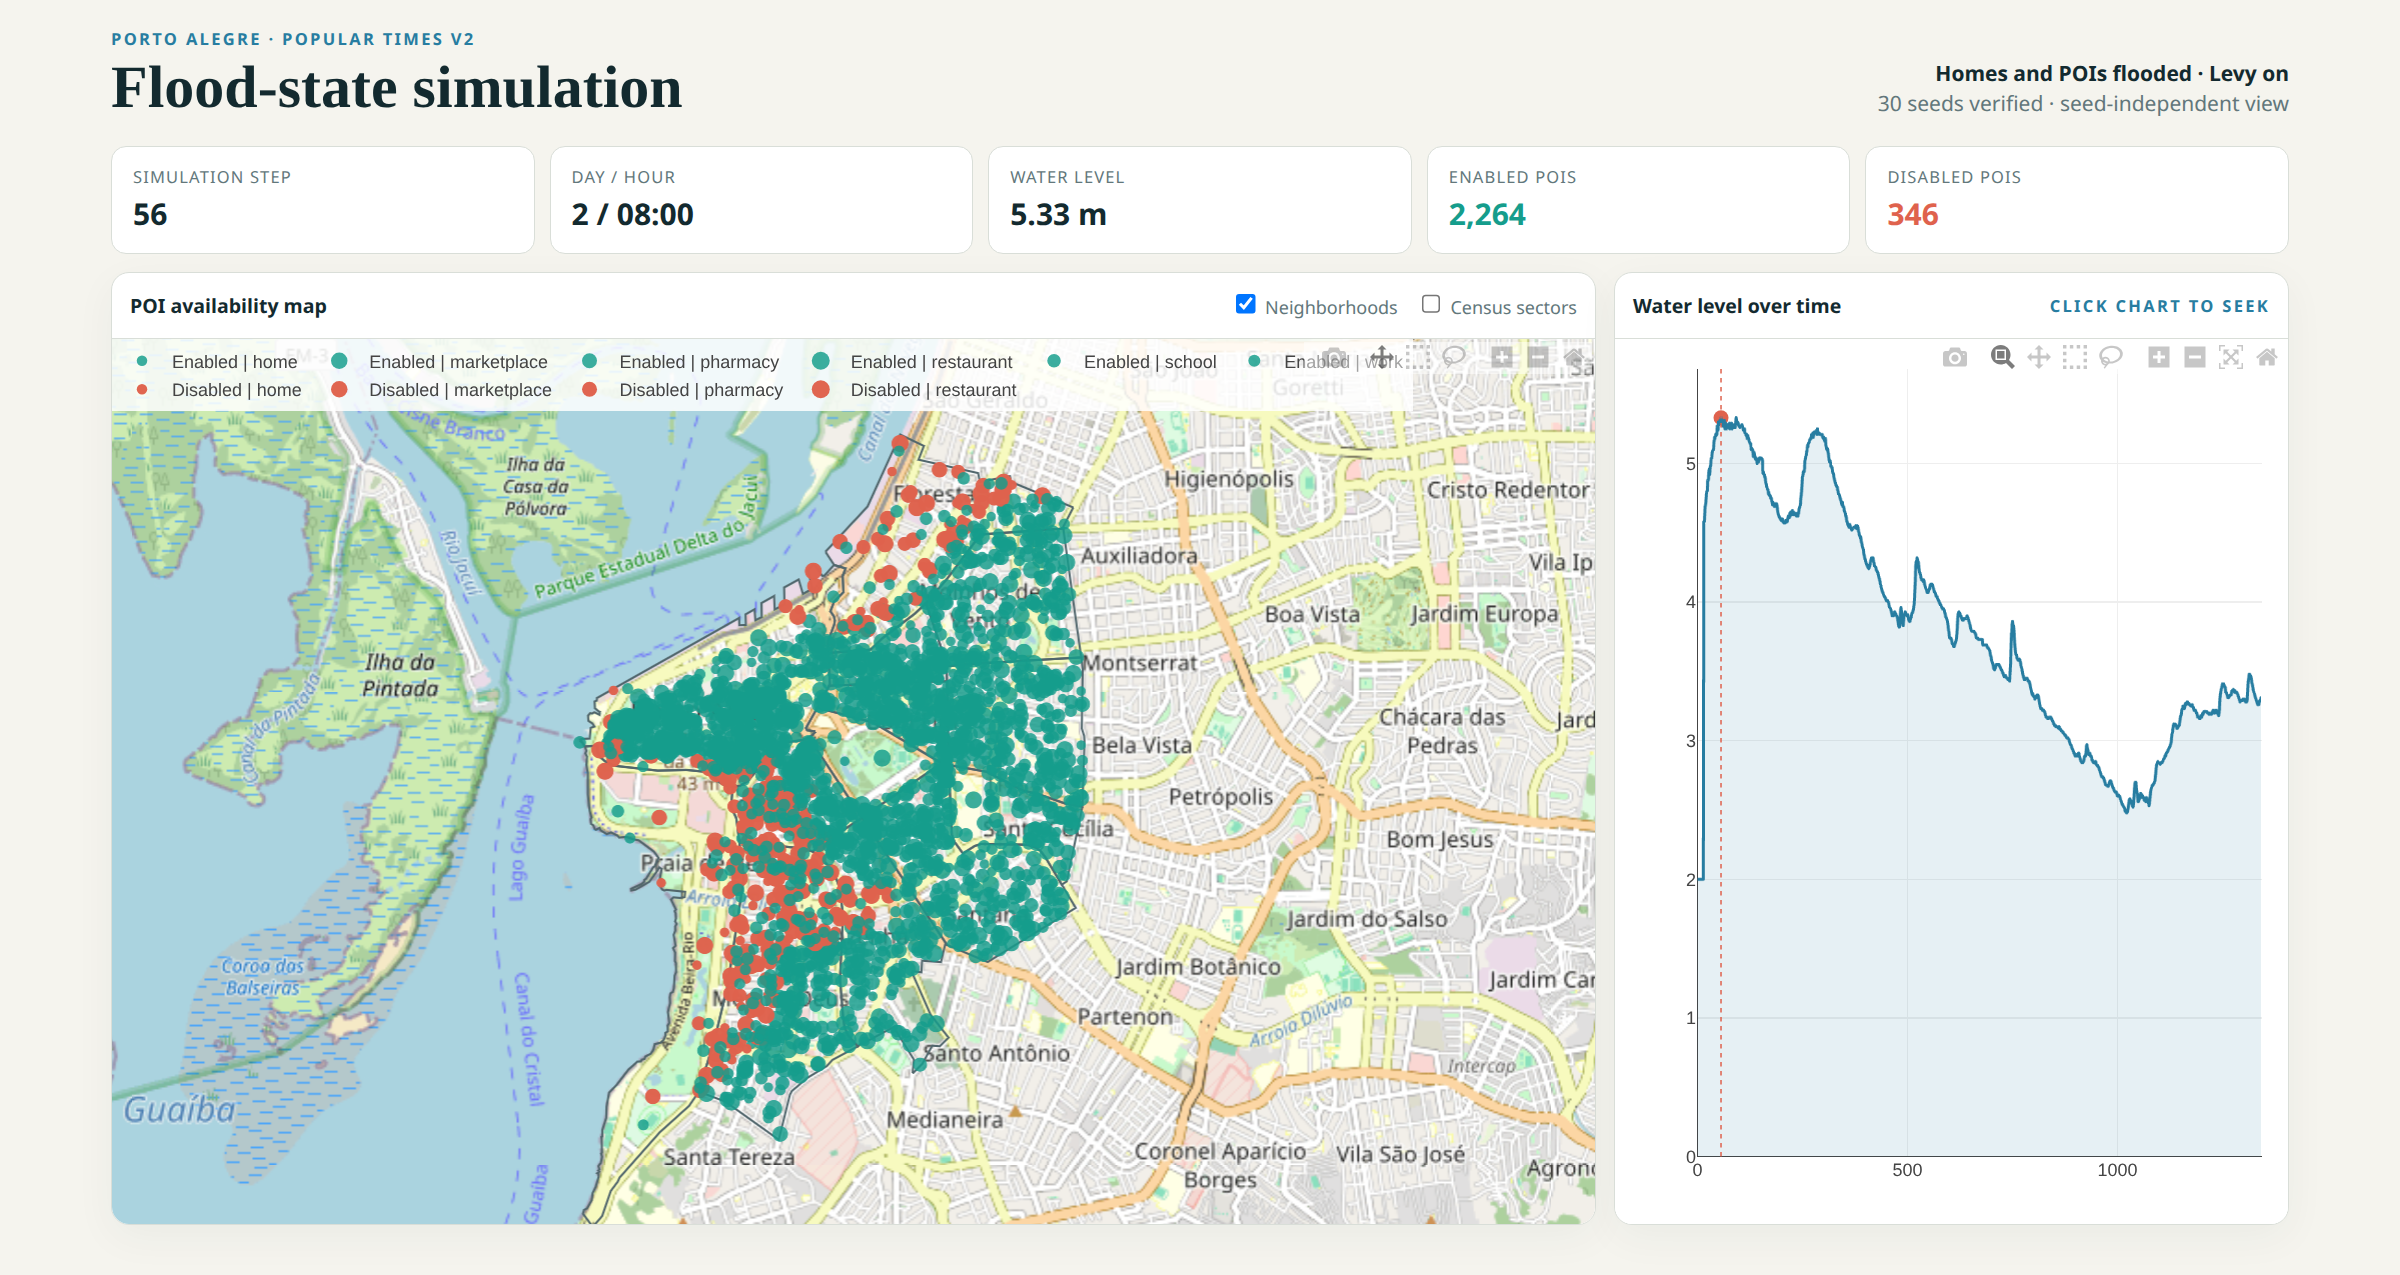
\includegraphics[width=0.99\textwidth]{fig/viz/flood_state_13_levy_both.png}
\caption{Flood-state snapshot for the reduced census-sector environment with L\'evy Walk enabled and the flood cause applied to home and activity $P$s. At simulation step 56 (day 2, 08:00), the historical sequence
%SO: sequence of what??????????????????????????????
reaches 5.33~m and makes 346 of the 2,610 modeled $P$s unavailable. The map distinguishes available $P$s from those carrying the flood disable cause.}
\label{fig:flood_state_visualization}
\end{figure}

\subsubsection{Shelter Locations and Capacities}

The shelter experiments examine whether populations displaced from flood-exposed areas can be redistributed to available emergency accommodation under spatial and capacity constraints. Their inputs, therefore, describe both the locations of shelters and the number of additional residents each shelter can accommodate.

The geographic coordinates, capacities, and occupancies of shelters were collected from the Abrigos RS website on May 15, 2024\footnote{Abrigos RS: \url{https://abrigosrs.org/}.}. The shelter locations were obtained from the geographic information available on the website. The collected input contains 128 tabular records with names, addresses, %SO: de pessoas?
coordinates, neighborhoods, capacities, occupancies, and free-text observations. After filtering and treatment of missing values, we consider 104 shelters with a combined capacity of 12,519 people and an initial occupancy of 10,963.

%SO: não gostei do proximo paragrafo. Re-escrevi. Validar
%The retained records are instantiated as $P$s of type \textit{shelter}. %SO: frase estranha retained records
%Their identifiers, %SO: their who? shelters? people?
%coordinates, reported capacities, and initial occupancies are stored through conventions for $\bm{\alpha}_i$ declared by the shelter plugin. Capacity and displacement parameters form $\bm{\theta}_{\Pi}$, while the handlers and hooks in $\mathcal{F}_{\Pi}$ and $\mathcal{H}_{\Pi}$ determine admission, denial, reallocation, and return behavior. These values therefore remain plugin-interpreted service state rather than universal fields with behavior fixed by the core environment.

The 104 shelters are represented as $P$s of type \textit{shelter}, with their geographic coordinates, capacities, and initial occupancies included as $P$ attributes ($ \ bm {\ alpha} _ i$). The shelter plugin uses these attributes together with scenario-specific capacity and displacement parameters ($\bm{\theta}{\Pi}$) to model the accommodation of displaced populations, including admission, denial due to capacity constraints, reallocation to alternative shelters, and return behavior. In this way, shelter-specific data and behavior are introduced through the plugin without modifying the general representation of $P$s in the LodusPop core model.

Figure~\ref{fig:shelter_locations_status} presents the locations and reported initial occupancy status of shelters with available capacity and occupancy information. The map makes visible both the uneven spatial distribution of shelter capacity and the limited number of places available before any simulated evacuation occurs.

\begin{figure}[ht]
\centering
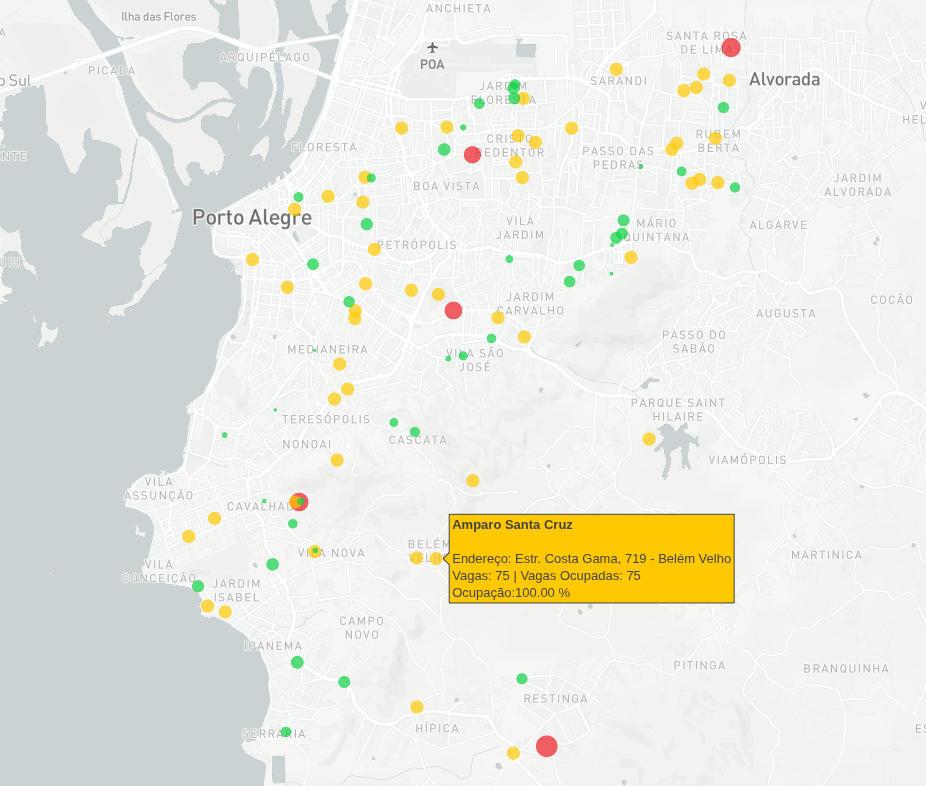
\includegraphics[width=0.85\textwidth]{fig/viz/shelters.png}
\caption{Shelter locations and reported initial occupancy status in Porto Alegre. Green markers identify shelters with available places, yellow markers identify shelters at their recorded capacity, and red markers identify shelters whose recorded occupancy exceeds their recorded capacity. Marker size is proportional to recorded capacity. The highlighted Amparo Santa Cruz record illustrates the address, capacity, occupied places, and utilization reported for an individual shelter.}
\label{fig:shelter_locations_status}
\end{figure}

\subsection{Health-Services}
\label{sec:infrastructure_input_data}

The health-service experiments examine access to recurring, capacity-constrained dialysis treatment in response to changes in demand and service availability. In addition to direct clinic disruptions, the scenarios represent dependencies on supporting water infrastructure, allowing failures at water-treatment facilities to indirectly affect access to dialysis services.

The dialysis environments represent Porto Alegre water-treatment stations (Estações de Tratamento de Água, ETAs) as $P$s of type \textit{water source} and dialysis facilities as $P$s of type \textit{dialysis clinic}. The complete overlay contains six ETAs and 12 clinics. ETA locations and the assignment of neighborhoods to water-supply systems were derived from maps and descriptions published by the Municipal Department of Water and Sewage (DMAE) and from a May 2024 account of water distribution and interconnections between the city's systems\footnote{DMAE water-system information: \url{https://prefeitura.poa.br/dmae/informacoes-agua}. GZH description of water distribution by neighborhood and connections between systems: \url{https://bit.ly/3TOMmnY}.}. The six ETAs reported by DMAE correspond to the six treatment stations represented in the complete environment.

%SO: muito hifen...
%Dialysis-clinic locations and clinic-to-water-source relations were provided by colleagues of the author based on their domain knowledge and the water-supply maps and sources cited above. Each clinic-to-source relation is represented by a dependency constraint in $D_i$, whereas names, coordinates, and external identifiers are stored in the relevant $P$ attribute mappings. Clinic opening and closing times and hourly treatment capacities are synthetic scenario parameters included in $\bm{\theta}_{\Pi}$.
Dialysis clinic locations and their relations to water sources were defined as inputs to the health service scenarios.\footnote{These data were compiled from the water supply maps and sources cited above, with support from project collaborators with domain knowledge.} Each relation between a clinic and a water source is represented by a dependency constraint in $D_i$, whereas names, coordinates, and external identifiers are stored in the relevant $P$ attribute mappings. Clinic opening and closing times, as well as hourly treatment capacities, are synthetic scenario parameters included in $\bm{\theta}_{\Pi}$.

%SO: re-escrevi para tirar cara de software
%The dialysis plugin uses $E_{\Pi}$ to declare the traceable characteristics required to represent patient selection, treatment frequency, due dates, status, origin, and treatment time. Its registered handler and time-step hook in $\mathcal{F}_{\Pi}$ and $\mathcal{H}_{\Pi}$ generate recurring demand, apply clinic capacity and schedule constraints, and perform treatment and return transitions.
The dialysis plugin uses $E_{\Pi}$ to define the traceable characteristics required to represent patient selection, treatment frequency, due dates, status, origin, and treatment time. Dialysis-specific behavior is represented through $\mathcal{F}{\Pi}$ and $\mathcal{H}{\Pi}$, including recurring treatment demand, clinic capacity and schedule constraints, treatment, and patient return.

%SO: re-escrevi. Valide
%The dialysis stress tests combine these service inputs with independent mechanisms for changing $P$ availability. A scheduled water-source outage adds its own direct cause to the source's $C_i(t)$, while flood exposure adds the distinct \textit{flood} cause to each affected source or clinic. The constraints $D_i$ then propagate source unavailability to dependent clinics. Removing one direct cause cannot restore a $P$ while another cause or an unsatisfied dependency remains. Synthetic sudden-rise water-level sequences, including transitions to 9.3~m and 10.1~m, are used as controlled stress conditions rather than observed hydrographs.
The dialysis stress tests combine these service inputs with various conditions that affect $P$ availability. Water source outages and flood exposure are represented as independent causes of unavailability in $C_i(t)$, allowing multiple disruption conditions to coexist. The dependency constraints $D_i$ propagate the unavailability of water sources to the dialysis clinics that depend on them. Consequently, a $P$ remains unavailable as long as at least one direct cause or dependency constraint prevents its operation. Synthetic water level sequences, including sudden increases to 9.3~m and 10.1~m, are used to create controlled stress conditions rather than to reproduce observed flood dynamics.

\end{comment}
\chapter{Experimental Results}
\label{chapter:experimental_results}

This chapter evaluates LODUS through experiments covering routine urban mobility, mobility under disruptions, and domain-specific applications. The results progress from the characterization of normal-life population movement to scenarios in which mobility, infrastructure, or service availability is altered.

The first section examines the spatial and temporal characteristics of normal-life mobility. The second evaluates population behavior under disruptions. Finally, epidemic-contagion and dialysis simulations demonstrate the use of the framework in application-specific scenarios involving additional population, infrastructure, and service dynamics. Detailed motivations, configurations, and analysis objectives are introduced within their respective sections.

%GA: Antiga intro do capítulo
%This chapter evaluates how the LodusPop abstractions support experiments with progressively different sources of population demand and state change. The experiments begin with recurring mobility, which provides the reference behavior for ordinary work, school, and activity visits, and then introduce large gatherings, epidemic processes, and environmental disruptions. The disruption scenarios are followed by shelter and dialysis simulations, which examine population displacement and the continuity of essential services when access, capacity, and infrastructure availability are constrained. Across these use cases, the emphasis is on controlled comparisons among explicit scenario configurations rather than on forecasting observed behavior in Porto Alegre.

\section{Normal-Life Mobility}

Normal-life mobility provides the reference condition for the experiments presented in this chapter. It represents recurring population movements performed under ordinary conditions, before the introduction of exceptional events, environmental disruptions or epidemic processes. Following the terminology introduced in Section~\ref{sec:normal_life}, these movements comprise \textit{commutes}, associated with work and school, and \textit{activities}, such as visits to marketplaces, restaurants, and pharmacies.

The experiments examine complementary spatial and temporal characteristics of normal-life mobility across the spatial representations introduced in Chapter~\ref{sec:simulation_environments_and_data}. They consider both the distribution of movements across space and the temporal organization of recurring demand, including the interaction between activity-related movement and regular work and school commutes.

Accordingly, this section addresses three main questions: (i) how normal-life movements are distributed spatially; (ii) how activity and commute demand varies over time; and (iii) whether these forms of mobility can operate concurrently while preserving their configured demand. These results establish the normal-life baseline used to interpret the additional population demands and disruptions introduced in the subsequent experiments.


\subsection{Experimental Overview}
\label{sec:routine_mobility_overview}

The experiments are organized into three sets. First, the neighborhood-level Lévy Walk experiments evaluate different mobility configurations. Second, the census-sector experiments examine recurring demand for marketplaces, restaurants, and pharmacies in the reduced and complete spatial representations. Third, the reduced census-sector environment combines these activities with explicit daily work and school commutes, allowing both forms of mobility to be evaluated within the same population.


All experiments use 24 simulation steps per cycle; in these experiments, one cycle represents one simulated day and each step represents one hour. The neighborhood-level experiments cover a single simulated day and focus on controlled changes to the Lévy Walk parameters. The census-sector experiments cover 56 days, corresponding to eight complete weeks, preserving complete weekly activity-demand cycles. Table~\ref{tbl:routine_mobility_scenarios} summarizes the principal configurations and comparisons.

% TODO: RESULTS-REFRESH: verify census-sector populations against
% thesis/normal_life/data/routine_mobility_summary.csv after rerunning.

\begin{table}[ht]
\centering
\footnotesize
\setlength{\tabcolsep}{4pt}
\caption{Normal-life mobility experiments and their principal comparisons.}
\label{tbl:routine_mobility_scenarios}
\begin{tabularx}{\linewidth}{@{}p{3.1cm}p{3.1cm}p{1.8cm}X@{}}
\toprule
\textbf{Experiment} &
\textbf{Environment} &
\textbf{Duration} &
\textbf{Principal comparison} \\
\midrule

Neighborhood-level Lévy Walk
& 94 neighborhoods; 94 home POIs; population 1,409,351
& 1 day
& Lévy scale values of 0.5, 1, 2, 5, and 10 are compared to examine spatial reach. A separate experiment holds the scale at 2 and varies movement restriction to examine changes in movement volume. \\

Activity baseline (reduced)
& Reduced census-sector; 13 regions; 435 home POIs; population 159,886
& 56 days
& Recurring marketplace, restaurant, and pharmacy activities are evaluated to characterize their spatial and temporal baseline in the reduced environment. \\ \\

Activity baseline (complete)
& Complete census-sector; 94 regions; 2,711 home POIs; population 1,331,414
& 56 days
& The same activity configuration is evaluated over the complete city representation, allowing comparison with the reduced environment. \\

Combined activities and attendance-controlled commutes
& Reduced census-sector; 13 regions; 435 home POIs; population 159,886
& 56 days
& Recurring activities are combined with explicit worker and student attendance demand to examine commute fulfillment and the spatial and temporal characteristics of both forms of mobility. \\

\bottomrule
\end{tabularx}
\end{table}

Because the reduced and complete census-sector environments represent different populations and spatial extents, comparisons between them emphasize normalized measures such as visits per resident, fulfillment, and travel distance rather than raw movement totals.

Together, these experiments provide the basis for examining normal-life mobility from three perspectives: the spatial distribution of movement, its temporal organization, and the interaction between recurring activities and work or school commutes.

\subsection{Spatial Characteristics of Normal-Life Mobility}
\label{sec:result_spatial_normal_life}

The spatial characteristics of normal-life mobility are examined at two complementary resolutions. The neighborhood-level experiments first evaluate how the configured Lévy Walk parameters affect the distance and volume of population movement across the city. The census-sector experiments then provide a finer representation in which the distances associated with recurring activities and work or school commutes can be analyzed separately.

This progression allows the spatial results to address two related questions. First, the neighborhood-level experiments examine how changes in mobility parameters modify the spatial reach of the generated movements. Second, the census-sector experiments characterize the distances produced by the different forms of normal-life mobility under the configurations adopted for activities and commutes. The former therefore provides a controlled analysis of the Lévy Walk configuration, while the latter examines the spatial patterns produced by the normal-life baseline used in the subsequent experiments.

\subsubsection{Neighborhood-Level Mobility}
\label{sec:routine_mobility_neighborhood}

The neighborhood-level experiments report the Lévy Walk analysis originally introduced with the published manuscript~\cite{silva2026lodusPop}. The full neighborhood representation of Porto Alegre is used, comprising 94 regions, 94 home POIs, and a population of 1,409,351. Population movements are generated in groups of 250 people, while travel distances are grouped into 500~m intervals. The experiments vary the Lévy scale while maintaining these remaining conditions unchanged, allowing its effect on the spatial reach of movement to be examined independently.

Figure~\ref{fig:routine_levy_distributions} presents the resulting displacement distributions for Lévy scale values of 0.5, 1, 2, 5, and 10. A displacement represents the movement of one person from an origin to a destination; consequently, a movement involving a group of 250 people contributes 250 displacements to the corresponding distance interval. Across the evaluated configurations, shorter movements are more frequent and progressively fewer movements occur at larger distances. Increasing the Lévy scale broadens this distribution, increasing the relative occurrence of longer-distance movements.

\begin{figure}[ht]
\centering
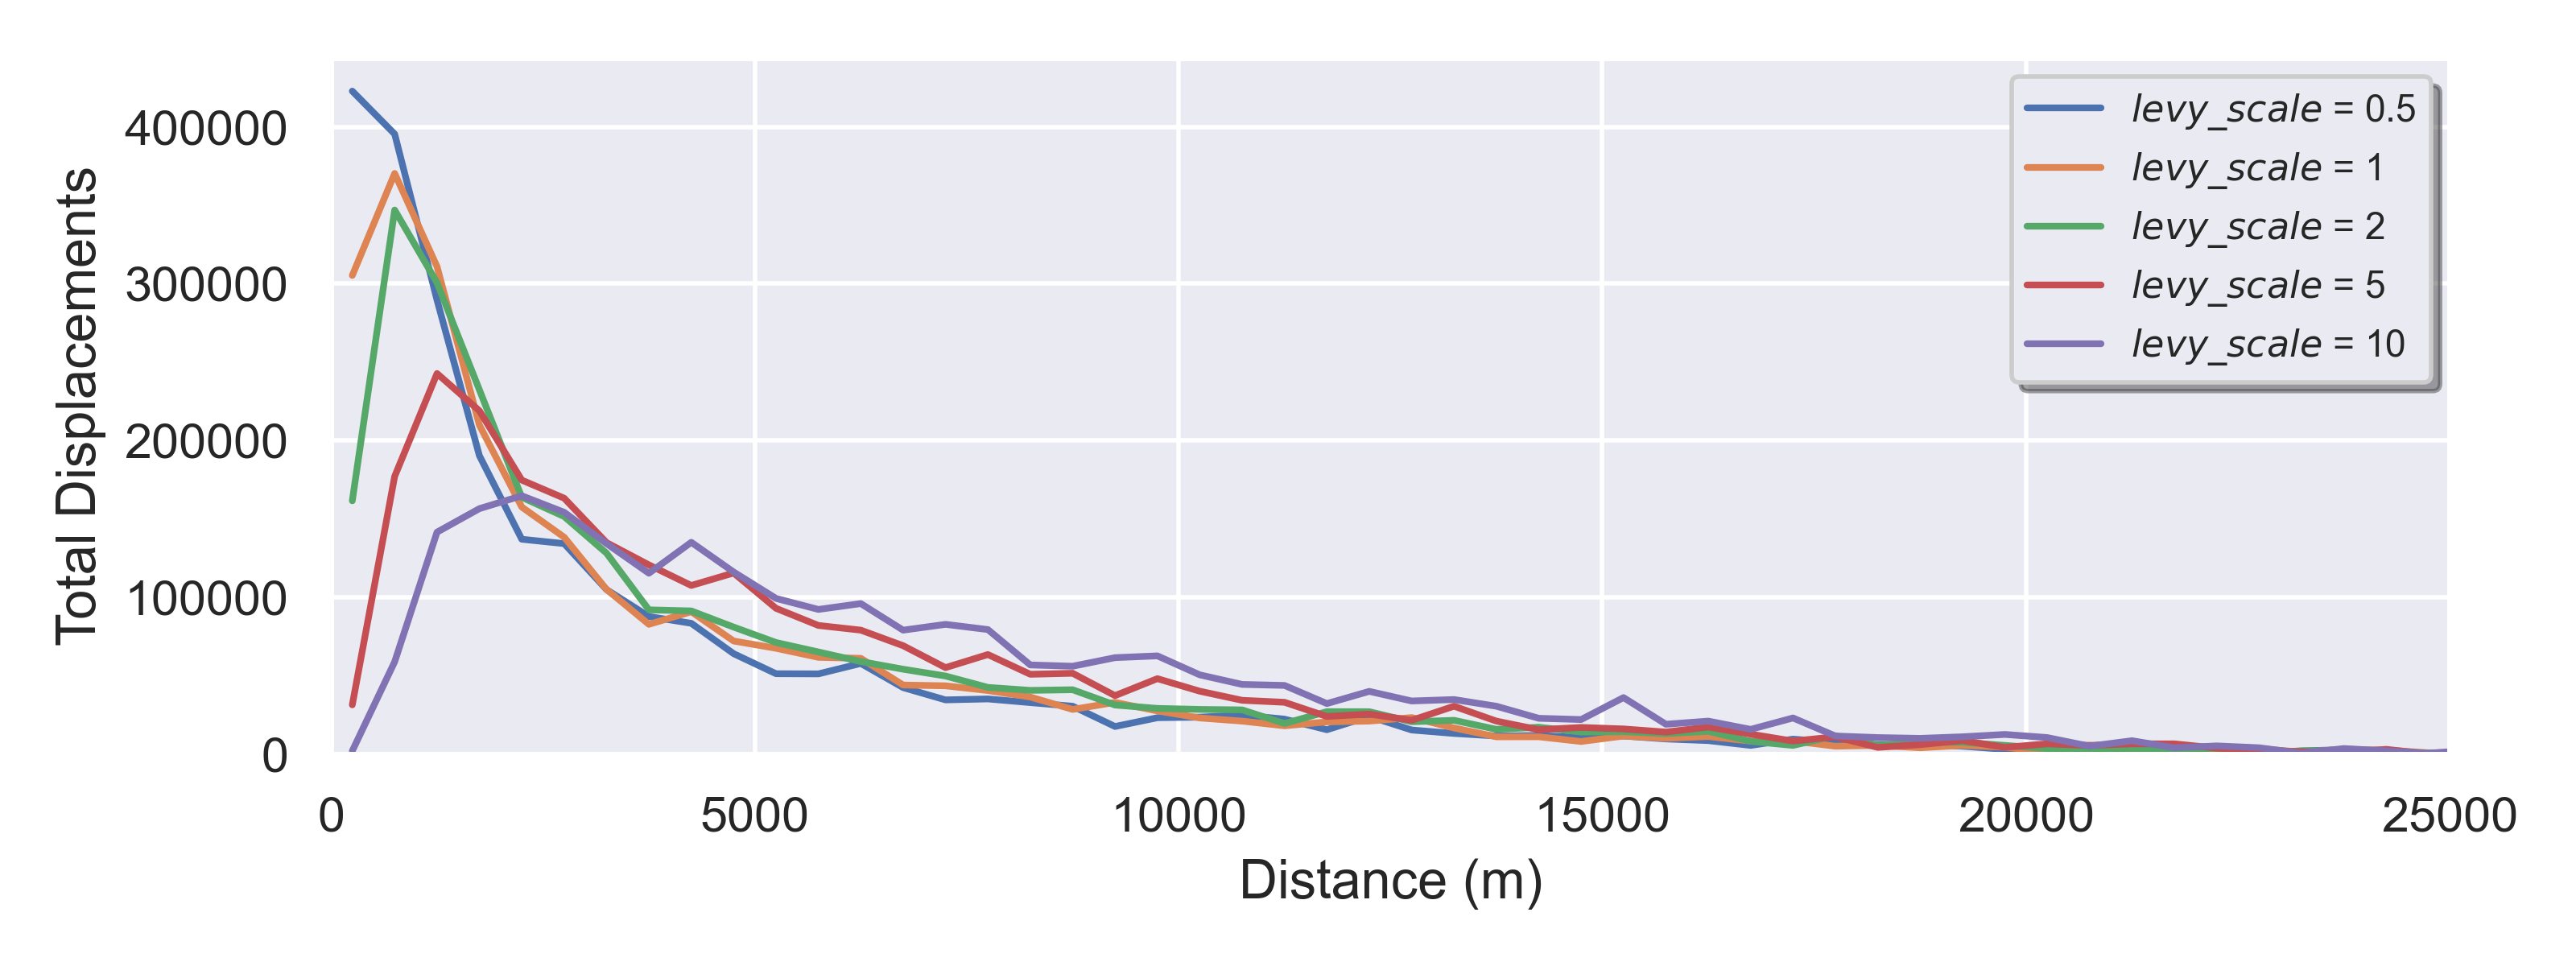
\includegraphics[width=0.98\linewidth]{fig/res-normal-life/Levy_Distributions.png}
\caption{Distribution of population displacements under different Lévy scale values in the neighborhood-level environment. Distances are grouped into 500~m intervals and movements are generated in groups of 250 people. Increasing the scale broadens the spatial distribution of movement.}
\label{fig:routine_levy_distributions}
\end{figure}

The configuration with a Lévy scale of 2 was adopted as the reference configuration for the subsequent neighborhood-level experiments. Under this configuration, approximately half of the generated displacements occur within 2~km of their origin, while the remaining movements extend over progressively larger distances. The resulting distribution therefore combines predominantly shorter movements with a smaller proportion of longer trips. The selected value represents a controlled mobility configuration rather than a calibration against observed travel distances in Porto Alegre.

A second experiment examines movement volume while maintaining the Lévy scale at 2. Figure~\ref{fig:routine_levy_restriction} compares the unrestricted condition with restriction values of 0.25, 0.50, and 0.75, corresponding to progressively stronger reductions in the population eligible to move. Unlike the Lévy scale, which changes the spatial distribution of destinations, movement restriction reduces the quantity of population participating in the routine while preserving the underlying distance configuration. As the restriction increases, the total displacement volume decreases accordingly.

\begin{figure}[ht]
    \centering
    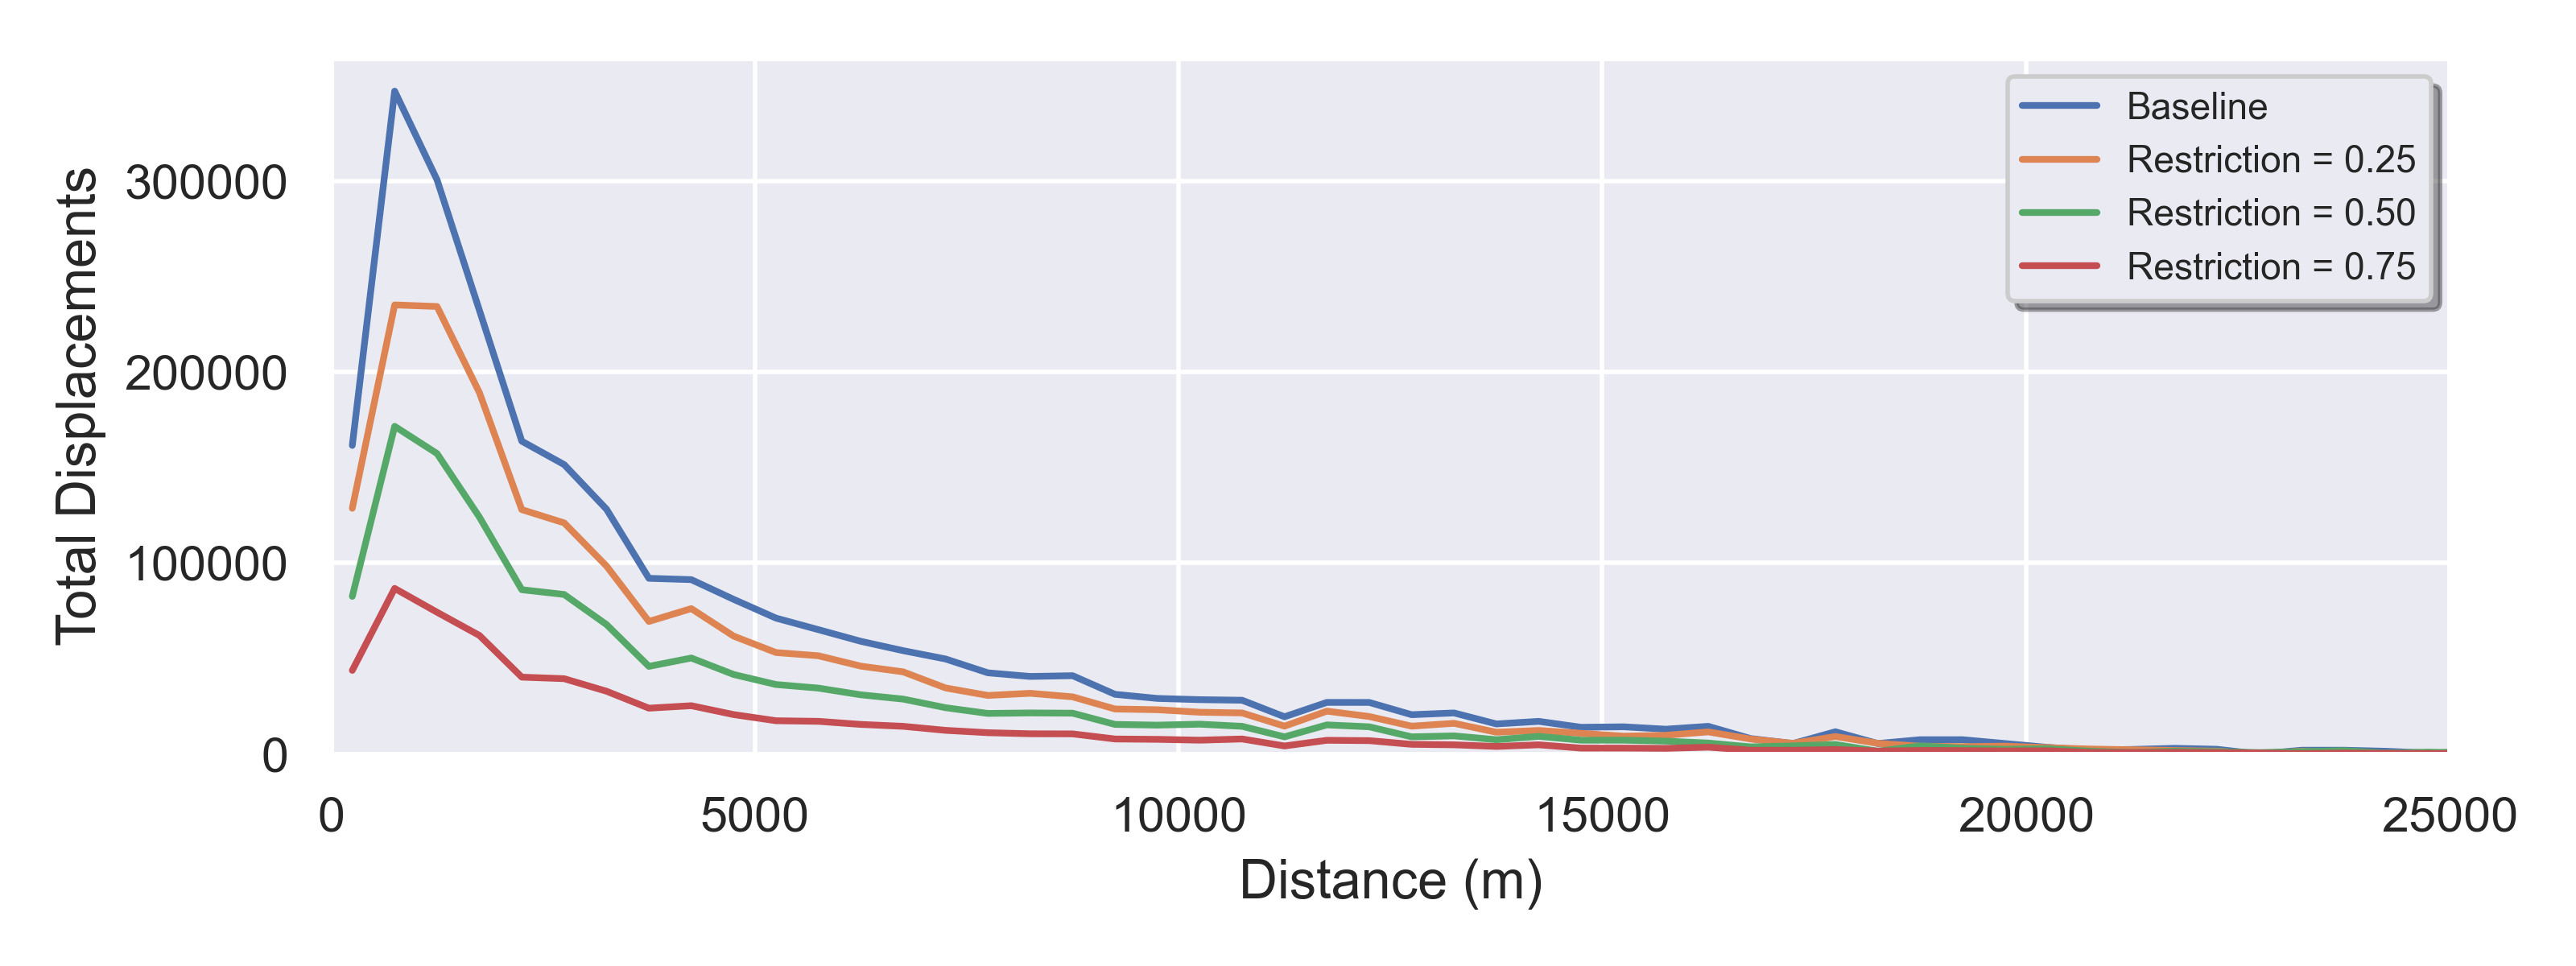
\includegraphics[width=0.98\linewidth]{fig/res-normal-life/MovementRestriction.png}
    \caption{Population displacement under different movement-restriction configurations in the neighborhood-level environment. The unrestricted condition is compared with restriction values of 0.25, 0.50, and 0.75, while the Lévy scale is held at 2.}
    \label{fig:routine_levy_restriction}
\end{figure}

Together, the experiments distinguish two dimensions of neighborhood-level normal-life mobility. The Lévy scale controls the spatial reach of the generated movements, whereas movement restriction controls their volume. The scale-2 configuration therefore provides the spatial reference adopted in the subsequent neighborhood-level experiments, while restriction allows the amount of population movement to be varied without changing the configured distance pattern.


\subsubsection{Census-Sector Mobility}
\label{sec:routine_mobility_census_sector}

The census-sector environments provide a finer spatial representation of normal-life mobility by distributing the population among multiple home POIs within each neighborhood. In these experiments, spatial movement can therefore be examined separately for \textit{activities}, corresponding to visits to marketplaces, restaurants, and pharmacies, and for \textit{commutes}, corresponding to work and school attendance. Unlike the neighborhood-level experiments, which evaluate how changes in the Lévy configuration affect spatial reach, the analysis here characterizes the distances produced by the normal-life configurations used in the census-sector environments.

Figure~\ref{fig:routine_mobility_distance_distribution} presents the distribution of travel distances for activities and commutes. Activity distance is measured between the source home from which population is selected and the corresponding activity destination, whereas commute distance is measured between the population's home and its work or school destination. These quantities therefore characterize different forms of movement and are analyzed separately.

Because individual movement records may represent population groups of different sizes, the distance distributions and summary statistics reported in this subsection are weighted by the number of people represented in each movement. Thus, a movement representing 50 people contributes proportionally more to the resulting distribution than a movement representing five people.

\begin{figure}[ht]
    \centering
    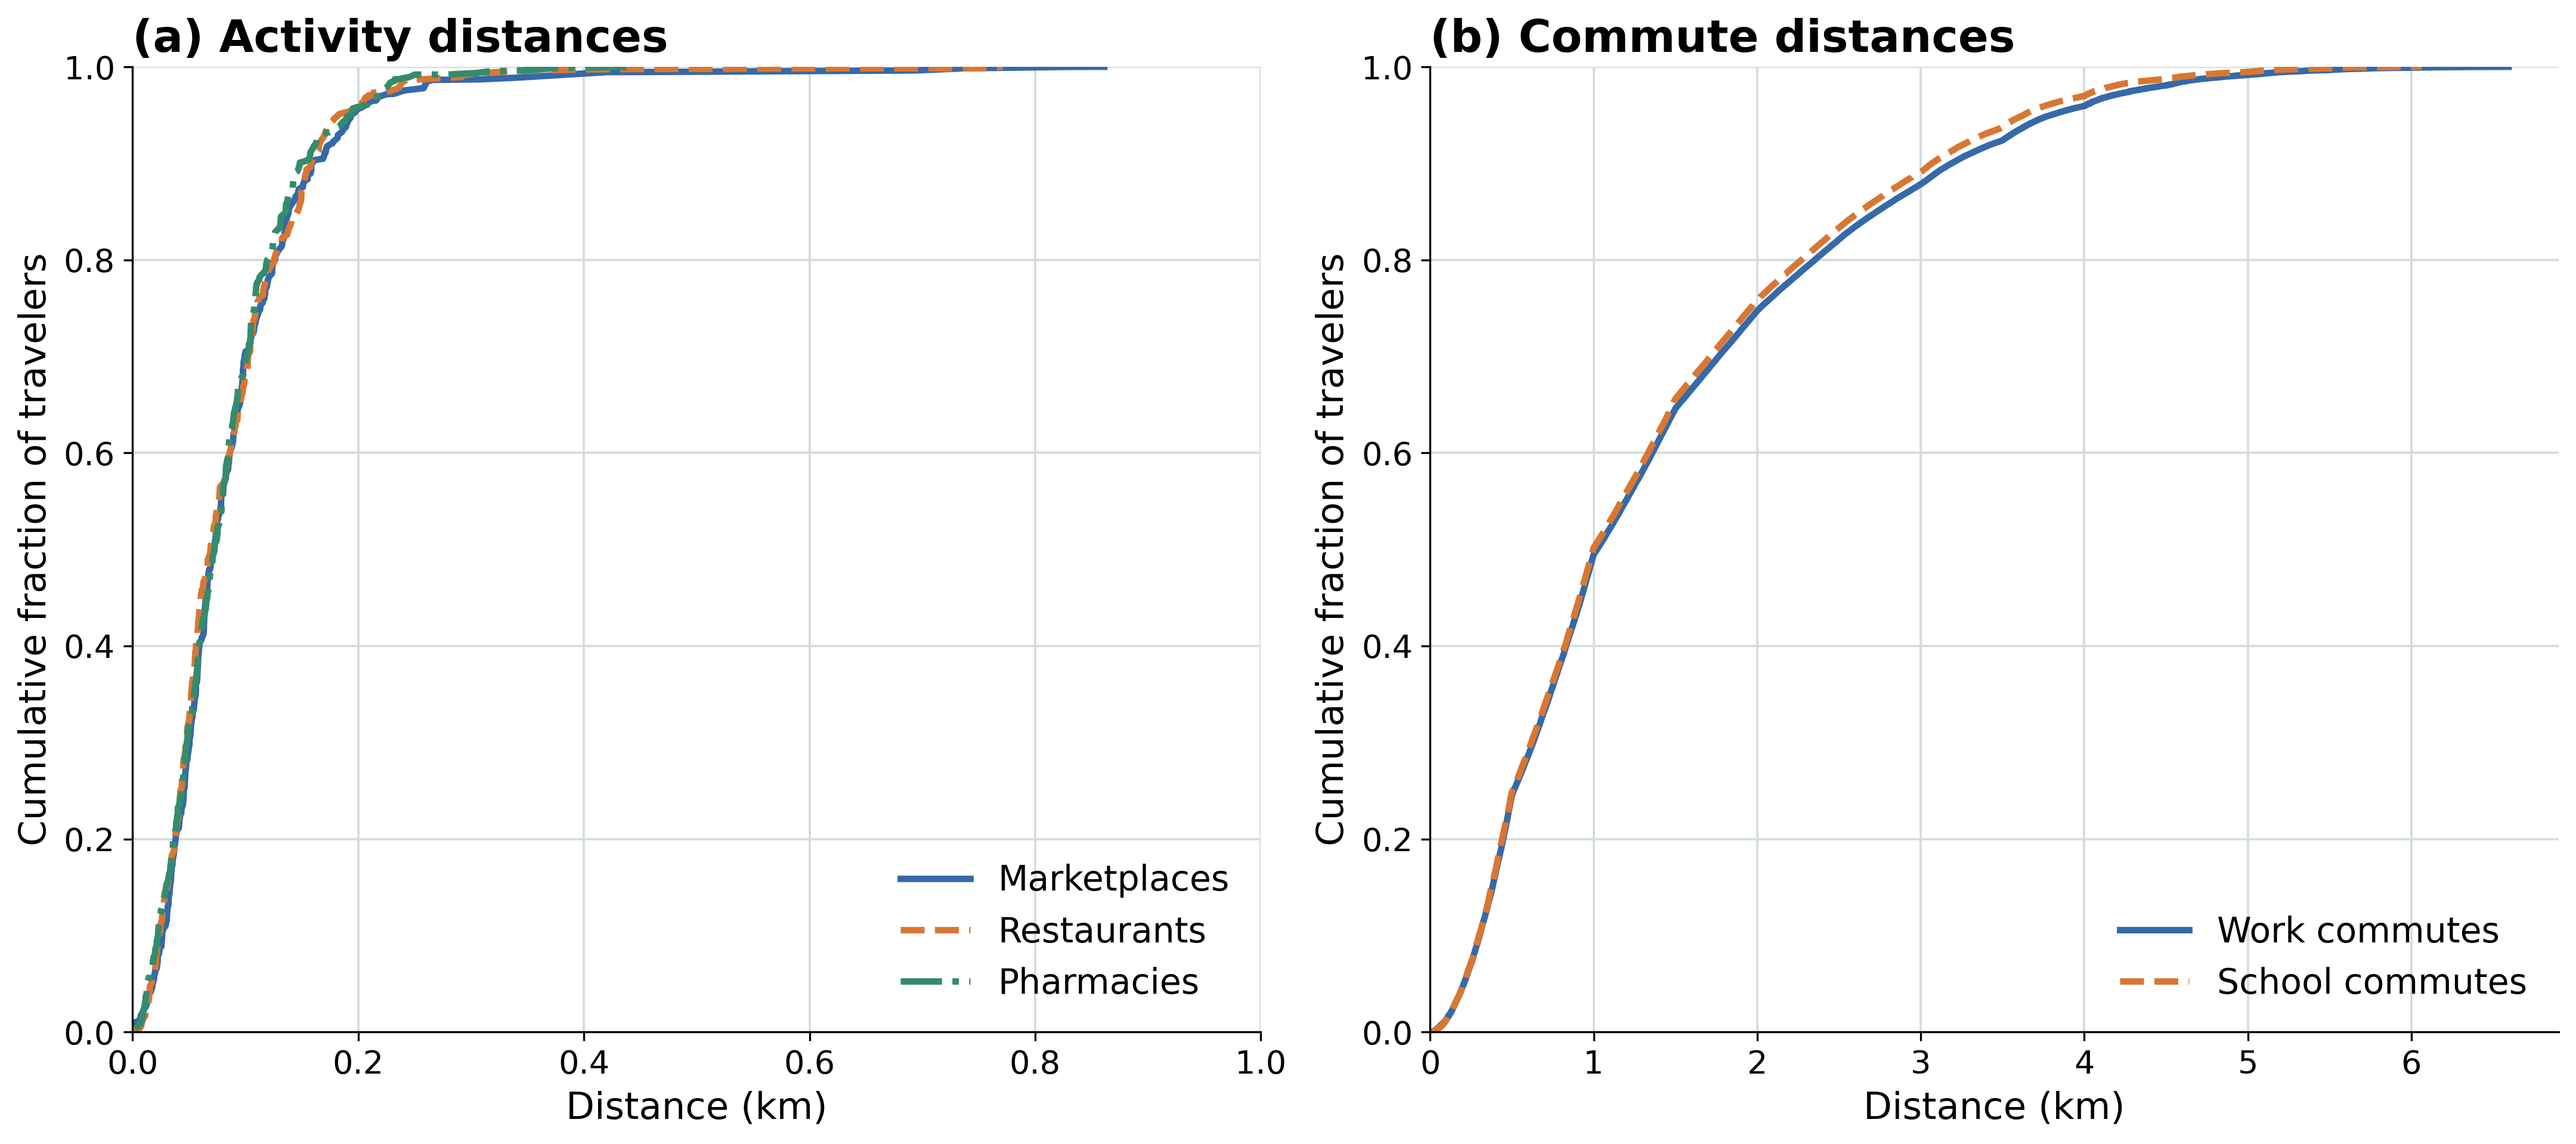
\includegraphics[width=\linewidth]{fig/res-normal-life/routine_mobility_distance_ecdf.png}
    \caption{Cumulative distributions of travel distances, weighted by the population represented in each movement considering 5 simulation runs of the reduced census-sector normal-life mobility experiment. (a) Activity distances between source homes and marketplace, restaurant, and pharmacy destinations. (b) Commute distances between homes and work or school destinations.}
    \label{fig:routine_mobility_distance_distribution}
\end{figure}

% TODO: RESULTS-REFRESH
In the reduced census-sector environment, activities are predominantly local relative to work and school commutes. In the combined normal-life mobility configuration, the mean activity distance is 86.53~m, whereas the mean commute distance is 1,411.15~m. Worker commutes are slightly longer on average, reaching 1,424.07~m, compared with 1,378.41~m for students. These results show that the two forms of normal-life mobility operate at different spatial scales under the evaluated configurations: recurring activities tend to draw population from nearby homes, while work and school attendance generates movement over a broader portion of the environment.

This difference is also visible beyond the means. Half of the population moved for activities travels no more than 70.75~m, and 90\% travels no more than 158.55~m. For worker commutes, the corresponding distances are 1,020.81~m and 3,188.05~m, while for student commutes they are 997.14~m and 3,069.00~m. Table~\ref{tbl:routine_mobility_distance_summary} summarizes these distributions, including the three activity destination types represented in Figure~\ref{fig:routine_mobility_distance_distribution}.

\begin{table}[ht]
\centering
\caption{Travel-distance statistics weighted by the population represented in each movement over 5 simulation runs of the combined normal-life mobility configuration in the reduced census-sector environment.}
\label{tbl:routine_mobility_distance_summary}
\begin{tabular}{@{}lrrr@{}}
\toprule
\textbf{Movement type} &
\textbf{Mean (m)} &
\textbf{Median (m)} &
\textbf{P90 (m)} \\
\midrule
All activities & 86.53 & 70.75 & 158.55 \\
\quad Marketplace & 89.08 & 72.00 & 159.59 \\
\quad Restaurant & 84.90 & 69.31 & 158.68 \\
\quad Pharmacy & 82.79 & 72.69 & 148.42 \\
Worker commutes & 1,424.07 & 1,020.81 & 3,188.05 \\
Student commutes & 1,378.41 & 997.14 & 3,069.00 \\
\bottomrule
\end{tabular}
\end{table}

The short activity distances are consistent with the spatial-selection configuration adopted for these visits, in which nearby eligible population is preferentially selected to satisfy demand at marketplace, restaurant, and pharmacy destinations. Commute destinations, in contrast, are distributed according to the configured distance-based movement process, producing a substantially wider distance distribution. The comparison should therefore be interpreted as a characteristic of the two normal-life mobility configurations rather than as an empirical estimate of travel behavior in Porto Alegre.

The three activity types have broadly similar distance distributions. Restaurants have the shortest median distance, at 69.31~m, while marketplaces have the broadest upper tail, with a 90th percentile of 159.59~m. Pharmacy visits have a slightly higher median of 72.69~m but the smallest 90th percentile, at 148.42~m. These relatively small differences indicate that the local sourcing pattern is shared across the three destination types.

The activity experiments are also executed in both the reduced and complete census-sector environments. Because these representations differ substantially in population and spatial extent, their raw movement totals are not directly comparable. The spatial comparison instead considers normalized measures and distance distributions to determine whether increasing the modeled extent of the city changes the characteristics of activity mobility.

In the activities-only baseline, the reduced environment produces a mean activity distance of 86.51~m, a median of 70.75~m, and a 90th percentile of 158.55~m. In the complete environment, these values increase to 89.88~m, 70.73~m, and 169.90~m, respectively. Thus, although the complete representation has a substantially larger population and spatial extent, activity sourcing remains predominantly local.

Overall, the census-sector results complement the neighborhood-level analysis by showing the spatial characteristics of the movements generated under the normal-life baseline itself. Activities and commutes occupy clearly different spatial scales, while the finer representation makes it possible to distinguish differences among destination types and between worker and student travel. These spatial patterns provide the basis for the temporal analysis presented next and, later, for evaluating how disruptions alter otherwise recurring mobility.


\subsection{Temporal Characteristics of Normal-Life Mobility}
\label{sec:routine_mobility_temporal}

In addition to operating at different spatial scales, activities and commutes follow different temporal patterns. Activity demand varies according to both the day of the week and the hour of the day, reflecting the temporal profiles associated with marketplaces, restaurants, and pharmacies. Work and school commutes instead follow daily attendance schedules, with different departure periods and durations for workers and students.

The census-sector experiments cover 56 simulated days, corresponding to eight complete weeks. This interval allows the weekly activity patterns to repeat eight times while also providing repeated daily commute cycles. The analysis therefore considers both when population movement is requested and, for commutes, how the population remains distributed at work and school before returning home.

\subsubsection{Activity Demand}
\label{sec:routine_mobility_activity_temporal}

The activity configuration produces recurring visits to marketplaces, restaurants, and pharmacies according to the weekly temporal profiles described in Section~\ref{sec:normal_life}. Over the eight simulated weeks, each resident is configured to generate one marketplace visit and one restaurant visit per week, together with 0.25 pharmacy visits per week. This corresponds to 18 requested activity visits per resident over the 56-day period.

% TODO: RESULTS-REFRESH
In the reduced census-sector environment, this configuration generates 2,877,888 activity requests: 1,279,088 marketplace visits, 1,279,088 restaurant visits, and 319,712 pharmacy visits. All requests are fulfilled under the normal-life baseline. The total corresponds to 17.9996 requested visits per resident, as defined by the configured weekly activity rates. %The small difference from exactly 18 results from allocating integer-valued demand among locations and hourly periods.

The aggregate totals, however, do not describe when these movements occur. Figure~\ref{fig:routine_activity_temporal_profiles} presents the distribution of requested activity visits according to weekday and hour for each destination type. The profiles produce distinct periods of higher and lower demand over the week, illustrating that normal-life activity movement is not distributed uniformly across simulation steps.

\begin{figure}[ht]
\centering
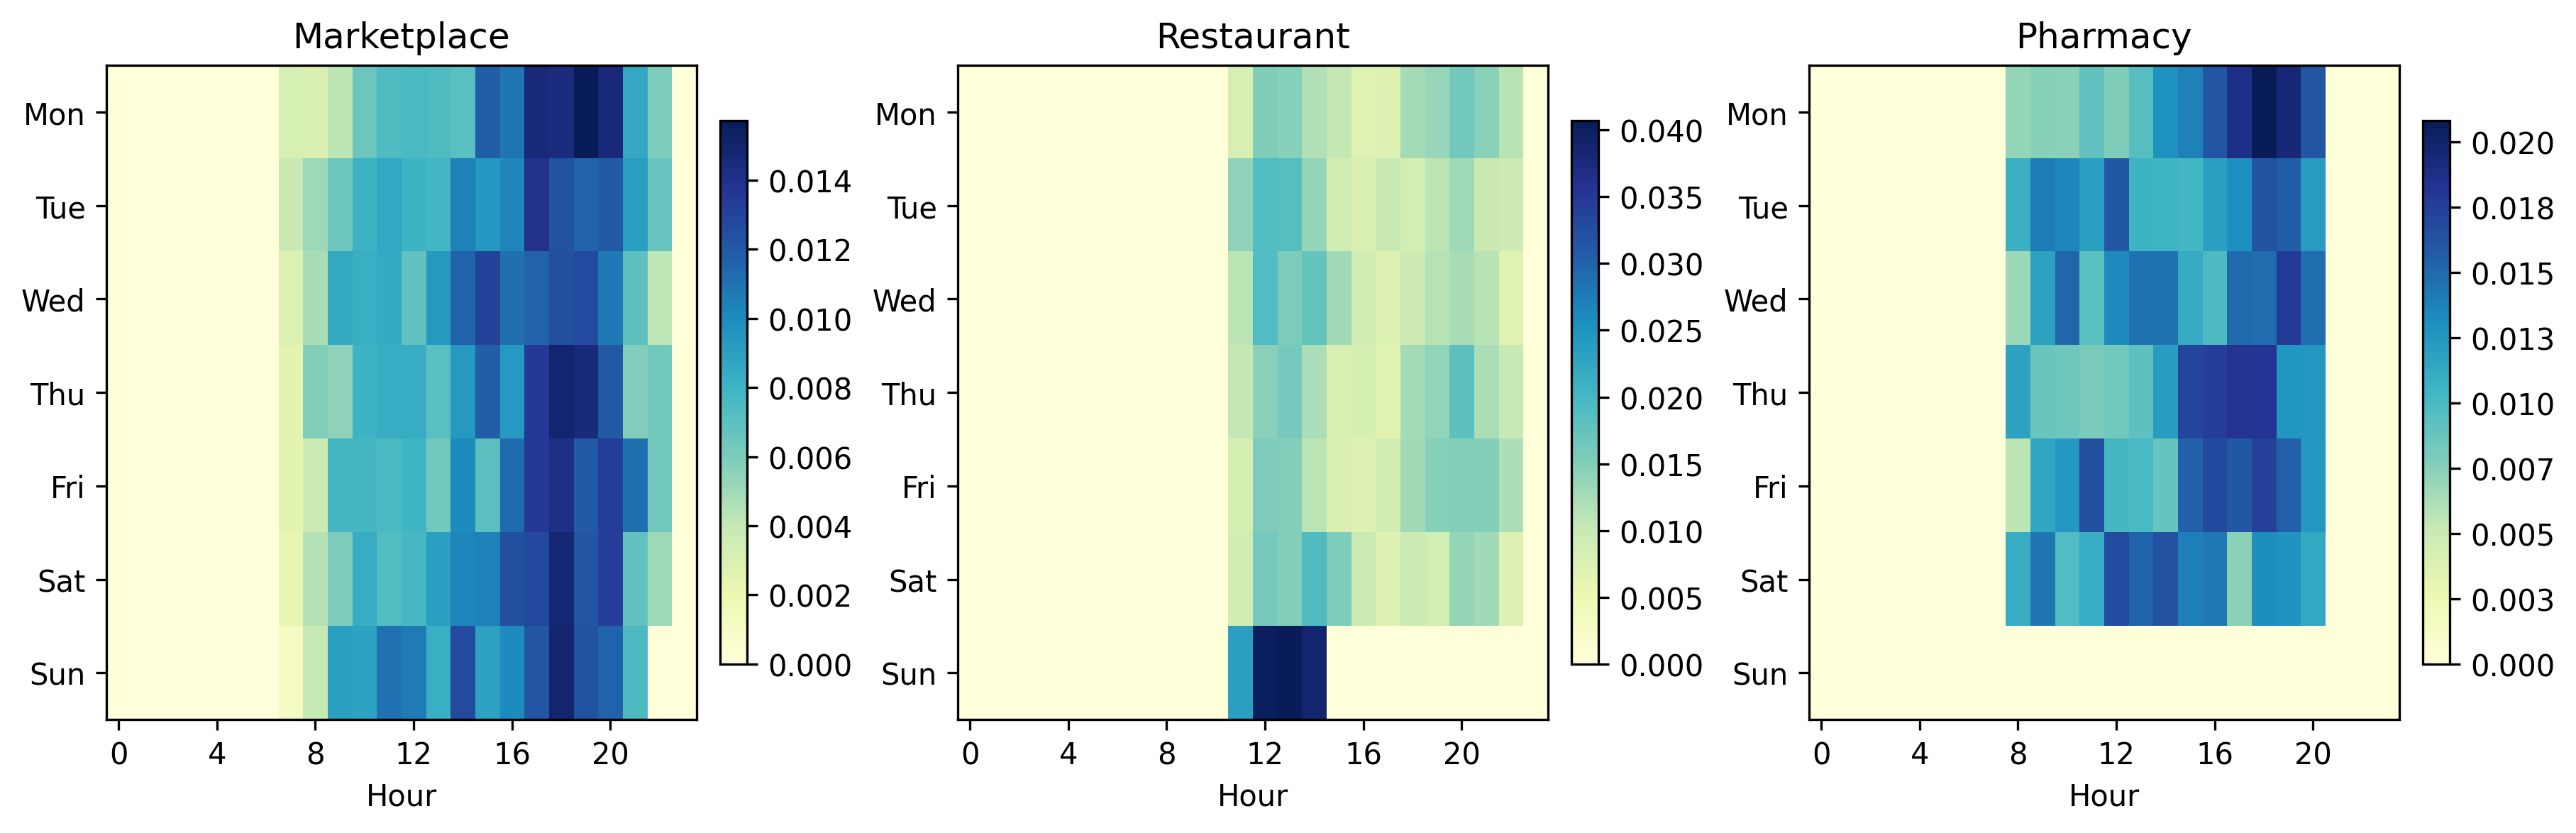
\includegraphics[width=\linewidth]{fig/res-normal-life/routine_activity_weekday_hour.png}
\caption{Temporal distribution of normal-life activity demand in the activities-only reduced census-sector baseline. Each cell reports its share of the corresponding activity type's requested visits over the eight-week simulation: (a) marketplaces, (b) restaurants, and (c) pharmacies. Normalizing within activity type makes the temporal shapes comparable despite their different total visit rates.}
\label{fig:routine_activity_temporal_profiles}
\end{figure}

Marketplace demand is distributed broadly from the morning into the evening on every day, with its largest weekday--hour value on Monday at 19:00. Restaurant demand has a more pronounced midday component and reaches its maximum on Sunday at 13:00. Pharmacy demand occurs from Monday through Saturday, is absent on Sunday in the configured profile, and reaches its maximum on Monday at 18:00. The heatmaps therefore show distinct weekly and hourly patterns even though all three activity types use the same local population-selection process.

The same temporal profiles are used in the reduced and complete census-sector environments. Their absolute request totals differ because the environments represent different populations, but the configured per-capita activity rates remain the same. %SO: acrescentei abaixo %GA: ok
In the complete environment, the 56-day simulation generates 23,965,416 requested activity visits, corresponding to 18 visits per resident (eight marketplace, eight restaurant, and two pharmacy visits), and all requests are likewise fulfilled.% In the complete environment, the 56-day simulation generates 23,965,416 requested activity visits, corresponding to 18 visits per resident, and all requests are likewise fulfilled. %Consequently, the temporal comparison between environments concerns the scale of demand rather than a change in the configured per-capita schedule.

These results establish the temporal activity demand of the normal-life baseline. Under conditions without disruptions or additional service constraints, the configured weekly demand is fully represented in both census-sector environments, while the weekday and hourly profiles determine when this population movement occurs.

\subsubsection{Work and School Commutes}
\label{sec:routine_mobility_commute_temporal}

% TODO: RESULTS-REFRESH
Work and school commutes introduce a different temporal structure. Across 5 simulation runs in the reduced census-sector environment, the occupation assignment produces a mean of 87,461.20 workers and 34,502.20 students. %Daily attendance is configured at 100\% for workers and students, producing mean daily demands of 87,461.20 worker commutes and 34,502.20 student commutes. 
The timing and duration of these movements differ between the two groups.

Worker departures are distributed across the configured daily departure profile, and workers remain at their destination for eight hours before returning home. Student departures are concentrated around three periods, at 08:00, 13:00, and 19:00, with students remaining at school for four hours. Figure~\ref{fig:routine_commute_temporal_behavior} presents these departure patterns together with the corresponding population occupying work and school destinations over the course of the day.

\begin{figure}[ht]
\centering
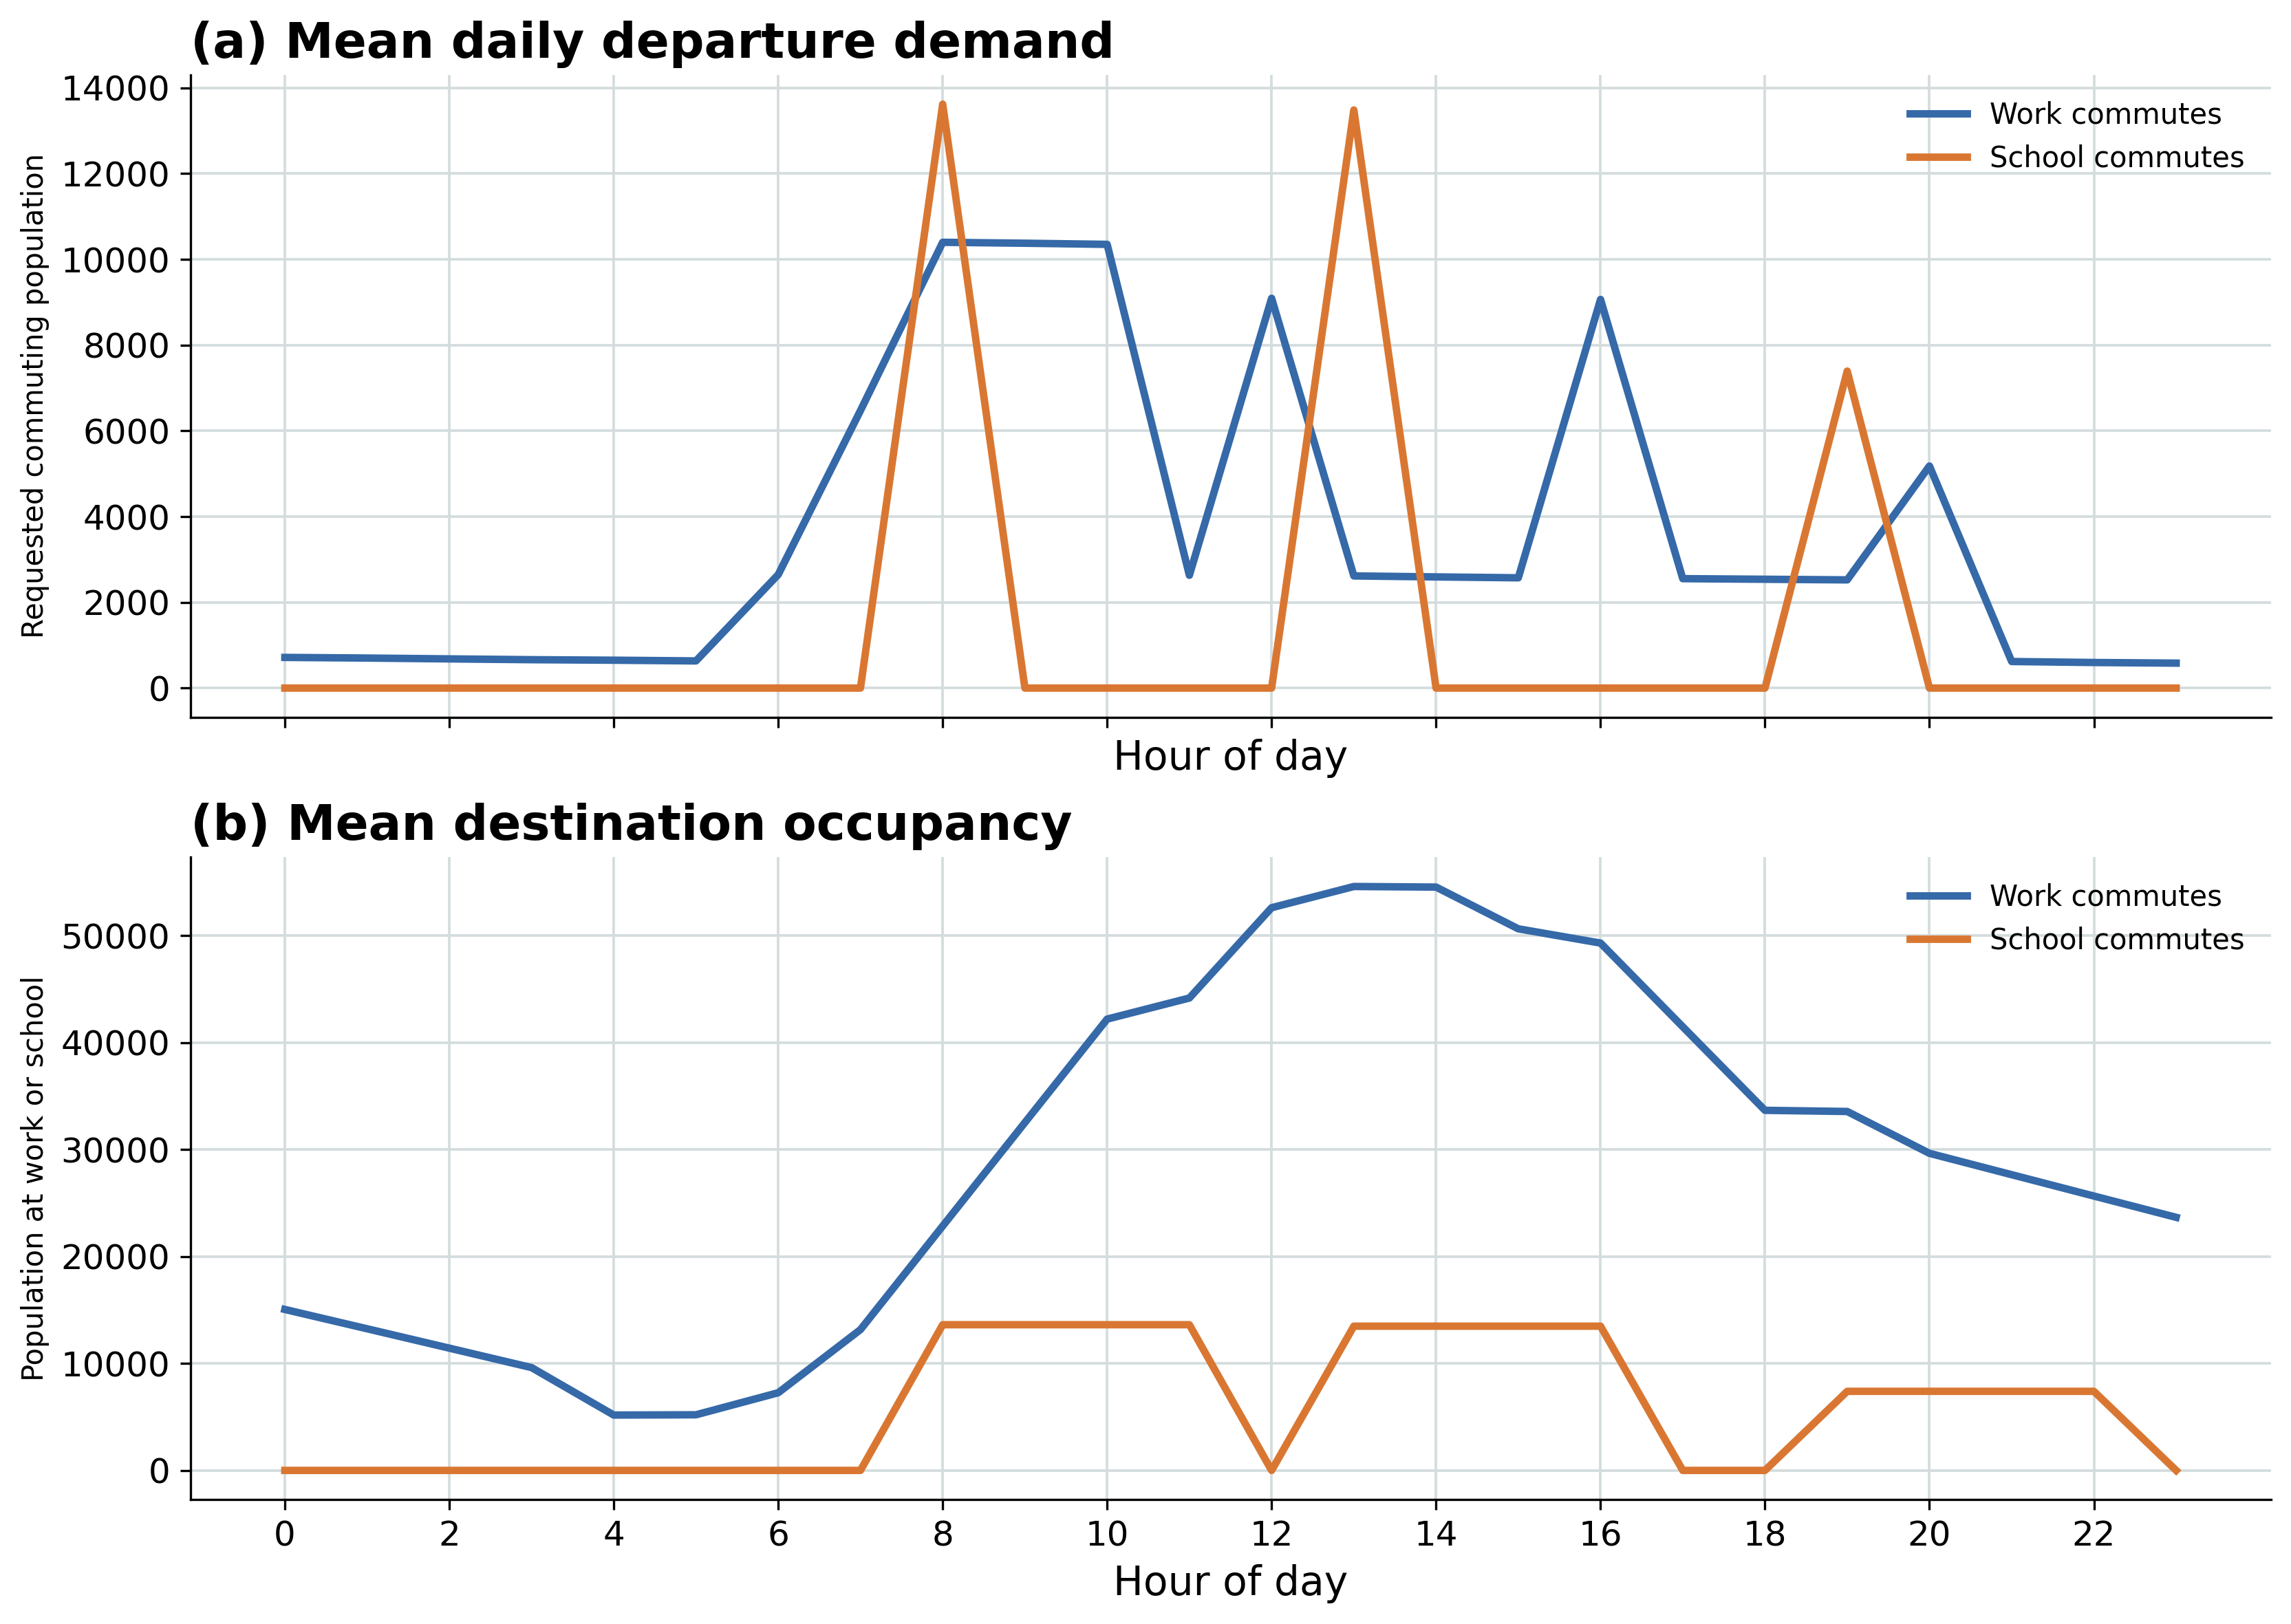
\includegraphics[width=\linewidth]{fig/res-normal-life/routine_commute_temporal_behavior.png}
\caption{Temporal characteristics of work and school commutes across 5 simulation runs in the reduced census-sector environment. (a) Mean daily requested commute population by departure hour. (b) Mean population occupying work and school destinations by hour, reflecting the departure schedules and respective eight-hour and four-hour stay durations.}
\label{fig:routine_commute_temporal_behavior}
\end{figure}

The departure and occupancy profiles describe complementary aspects of commute behavior. Mean departure demand is highest at 08:00 for both groups, reaching 10,399.20 requested workers and 13,621.40 requested students per day. Because workers remain away for eight hours and departures occur throughout the day, work occupancy accumulates into a broad daytime period and reaches its maximum at 13:00, when a mean of 54,590.20 workers are at work. School occupancy instead forms three four-hour periods beginning at 08:00, 13:00, and 19:00. Their mean occupancies are 13,621.40, 13,486.00, and 7,394.80 students, respectively, with the morning period producing the maximum.

%Across the 56 simulated days, the combined attendance configuration produces a mean of approximately 6.83 million commute requests per simulation run, of which only a mean of 2.80 people remains unmet. 
Across the 56 simulated days, the combined attendance configuration produces a mean of approximately 6.83 million requested commute movements per simulation run. Of the population associated with these requests, a mean of only 2.80 people per run remains unmet.
Across all 5 runs, the total unmet population is 14 people: 14 workers and no students. In each case, the corresponding origin did not contain enough eligible population to provide the complete requested group when the commute was processed. Thus, commute demand is almost completely fulfilled under normal-life conditions, although worker fulfillment is not strictly complete.

Overall, the temporal results distinguish the two principal forms of normal-life mobility. Activity demand follows recurring weekly patterns that vary by destination type, whereas work and school mobility is organized around daily attendance schedules and different periods spent away from home. These patterns complement the spatial differences identified in the previous subsection and provide the temporal reference against which later changes in population mobility can be evaluated.



\subsection{Combined Normal-Life Mobility}
\label{sec:routine_mobility_combined}

The previous analyses consider the spatial and temporal characteristics of activities and commutes separately. The final normal-life experiment examines these movements together in the reduced census-sector environment. In this configuration, recurring visits to marketplaces, restaurants, and pharmacies occur over the same represented population that performs daily work and school commutes. The objective is to determine whether both forms of mobility can coexist while preserving their configured demand and return patterns.

% RESULTS-REFRESH: update fulfillment values and Table~\ref{tbl:routine_mobility_fulfillment_summary}
% from thesis_result_table.csv after rerunning.
The addition of work and school commutes does not reduce the configured activity demand under the normal-life baseline. In each 56-day run, the activity configuration generates 2,877,888 requests, all of which are fulfilled. This corresponds to 17.9996 visits per resident, the same rate observed in the activities-only baseline.

At the same time, work and school attendance is almost completely fulfilled. Across the 5 attendance-controlled runs, mean requested commute demand is approximately 6.83 million people per run, with a mean unmet demand of only 2.80 people. As summarized in Table~\ref{tbl:routine_mobility_fulfillment_summary}, unmet demand is concentrated among workers, with a mean of 2.80 unmet people per run, while students account for 0.00 per run.

\begin{table}[ht] 
    \centering 
    \caption{Movement demand and fulfillment in the combined reduced-environment normal-life configuration. Activity values are constant totals per 56-day run; commute values are means across 5 runs.} 
    \label{tbl:routine_mobility_fulfillment_summary} 
    \begin{tabular}{@{}lrrr@{}} 
    \toprule 
    \textbf{Movement type} & \textbf{Requested} & \textbf{Fulfilled} & \textbf{Unmet} \\ \midrule 
    Activities & 2,877,888.00 & 2,877,888.00 & 0.00 \\ 
    Worker commutes & 4,897,827.20 & 4,897,824.40 & 2.80 \\ 
    Student commutes & 1,932,123.20 & 1,932,123.20 & 0.00 \\ 
    All commutes & 6,829,950.40 & 6,829,947.60 & 2.80 \\ \bottomrule 
    \end{tabular}
\end{table}

Thus, the simultaneous presence of activities and commutes does not produce a meaningful reduction in either form of normal-life demand under the evaluated conditions. This is relevant because both processes draw from the same represented population: people attending work or school may be away from their home locations when activity demand occurs, while activity visits temporarily remove additional population from available origins. Nevertheless, the normal-life configuration retains sufficient eligible population to satisfy essentially all requested movement.

% TODO: RESULTS-REFRESH
The spatial sourcing of activity visitors also remains effectively unchanged when attendance-controlled commutes are introduced. The mean activity distance changes from 86.51~m in the activities-only baseline to 86.53~m in the combined configuration, while both have a median of 70.75~m and a 90th percentile of 158.55~m. Thus, introducing daily work and school commutes does not meaningfully alter either the fulfillment or the spatial characteristics of recurring activity demand under the evaluated normal-life conditions.

The combined experiment therefore establishes a normal-life condition in which recurring activities and daily commutes coexist within the same population representation. Their distinct spatial and temporal characteristics are retained while their requested movements remain almost entirely satisfied. This condition provides the reference against which subsequent experiments can examine how exceptional demand, environmental disruptions, and service constraints alter population mobility.

\subsection{Main Findings}
\label{sec:routine_mobility_findings}

The normal-life experiments establish a reference pattern of recurring population movement before additional events or disruptions are introduced. At the neighborhood level, changes to the Lévy scale alter the spatial reach of movement, while movement restriction independently controls the volume of population displaced. The adopted scale-2 configuration favors comparatively short movements relative to the range of distances represented in the neighborhood-level environment while retaining a smaller proportion of longer trips.

At census-sector resolution, activities and commutes exhibit distinct spatial characteristics. Half of activity movements occur within 70.75~m, compared with 1,020.81~m for workers and 997.14~m for students. Worker and student mobility also differ temporally, with their configured departure periods and stay durations producing different daily patterns of destination occupancy.

Activity demand additionally follows recurring weekday and hourly patterns that differ among marketplaces, restaurants, and pharmacies. Work and school movement instead follows daily attendance schedules, generating temporal patterns associated with departures, time spent at destinations, and returns. Together, these results show that normal-life mobility is not represented by a single homogeneous movement process, but by forms of recurring mobility operating at different spatial and temporal scales.

Finally, the combined baseline shows that these movements can occur concurrently without materially reducing their fulfillment under the evaluated conditions. Activity demand remains fully satisfied, while only a mean of 2.80 people remains unmet among approximately 6.83 million commute requests per run.

These results establish the spatial distribution, temporal organization, and demand fulfillment of the normal-life mobility used as a reference throughout the remaining experiments. The following sections depart from this condition by introducing additional population demand and changes in the availability or operation of modeled locations, allowing their effects to be interpreted relative to the recurring mobility characterized here.

%GA: TODO trecho da Soraia
The quantitative results reported in these experiments should be interpreted as outcomes of the configured mobility models rather than as empirical estimates of mobility behavior in Porto Alegre. While the modeled population and spatial environment are derived from real-world data, activity frequencies, attendance schedules, destination-selection mechanisms, and other behavioral parameters reflect modeling assumptions adopted for the experiments. Therefore, quantities such as the number of requested visits, commute demand, and travel distances are not expected to reproduce observed mobility statistics directly. Nevertheless, the resulting values provide a plausibility check on the simulated scenarios, ensuring that the generated mobility remains within reasonable orders of magnitude for the represented population while preserving the behavioral patterns defined by each configuration.



\section{Exceptional Events and Environmental Disruptions}
\label{sec:results_exceptional_events_disruptions}

The preceding section characterized recurring population movement under normal-life conditions. The experiments in this section introduce temporary conditions that depart from this reference in two complementary ways. Large-scale events introduce exceptional demand for movement toward specific locations and times, while environmental disruptions change the availability of locations used by the population and may suppress, redirect, or generate additional movement.

Three experiment groups are considered. First, large-scale-event scenarios examine how gathering demand changes population displacement according to event location, the number of concurrent events, and their timing. Second, flood scenarios evaluate how unavailable origins and destinations affect recurring activities and work or school commutes, including the substitution of unavailable activity destinations. Finally, shelter scenarios examine population movement toward capacity-constrained facilities in response to environmental exposure.

Accordingly, this section addresses three main questions: (i) how exceptional gathering demand alters population movement when multiple events occur within the same urban population; (ii) how environmental disruption changes the fulfillment of recurring mobility and what additional burden is introduced by destination adaptation; and (iii) how evacuation demand, shelter capacity, reallocation, and facility disruption affect the protection of exposed populations.


\subsection{Experimental Overview}
\label{sec:exceptional_disruption_overview}

The experiments use the spatial representations introduced in Section~\ref{sec:spatial_representations}. The large-scale-event and shelter experiments use the neighborhood-level environment, whereas the flood-mobility experiments use the reduced and complete census-sector environments. Their durations and outcome measures also differ according to the phenomenon being evaluated. Table~\ref{tbl:exceptional_disruption_scenarios} summarizes the principal comparisons.

\begin{table}[ht]
\centering
\footnotesize
\setlength{\tabcolsep}{4pt}
\caption{Exceptional-event and environmental-disruption experiments and their principal comparisons.}
\label{tbl:exceptional_disruption_scenarios}
\begin{tabularx}{\linewidth}{@{}p{2.9cm}p{3.4cm}p{1.7cm}X@{}}
\toprule
\textbf{Experiment} &
\textbf{Environment} &
\textbf{Duration} &
\textbf{Principal comparison} \\
\midrule

Large-scale events
& Neighborhood-level; 94 regions; population 1,409,351
& 1 day
& No-event baseline and combinations of one to four events are compared to examine event location, concurrent demand, and simultaneous versus staggered execution. \\

Activity disruption
& Reduced and complete census-sector environments
& 56 days
& No exposure is compared with unavailable activity destinations, unavailable homes, and combined exposure to evaluate activity-demand suppression. \\

Flood-aware commuting
& Reduced and complete census-sector environments
& 56 days
& Unavailable homes and destinations are compared to examine their effects on worker and student commute fulfillment. \\

Activity adaptation
& Reduced and complete census-sector environments
& 56 days
& Combined exposure with activity suppression is compared with nearest-available same-type destination substitution. \\

Shelter evacuation
& Neighborhood-level with 104 added shelters; population 1,409,351; mapped exposed population 182,936
& 14 days
& Reallocation, response rate, exposure magnitude, shelter capacity, and selected facility failures are compared. \\

\bottomrule
\end{tabularx}
\end{table}

Because these experiment groups differ in spatial representation, duration, population, and demand definition, their raw outcome quantities are not compared directly across each other. Instead, each set of experiments is evaluated relative to its corresponding reference condition and using the measures appropriate to the simulated process.


\subsection{Large-Scale Events}
\label{sec:results_large_scale_events}

Large-scale events introduce occasional concentrations of population that coexist with the normal-life mobility described in Section~\ref{sec:routine_mobility_neighborhood}. The experiments in this subsection evaluate how these additional demands affect population displacement when the destination, number of concurrent events, and event timing are varied. The gathering mechanism and its configuration are described in Section~\ref{sec:gather_population_plugin_inputs}.

The results correspond to the large-scale-event experiments originally reported with the published manuscript~\cite{silva2026lodusPop}. 
The experiments use the neighborhood-level representation of Porto Alegre, comprising 94 regions, 504 POIs, and a population of 1,409,351. Each simulation covers one 24-hour cycle and uses the neighborhood-level normal-life mobility configuration with a L\'evy scale of 2.

Four event destinations are considered:

\begin{itemize}
    \item Event A: a sports event at the stadium in Farrapos;
    \item Event B: a sports event at the stadium in Praia de Belas;
    \item Event C: a commercial event at the marketplace in Centro Hist\'orico; and
    \item Event D: a cultural event at the university represented by the school POI in Partenon.
\end{itemize}

Figure~\ref{fig:large_event_locations} shows the neighborhoods containing these destinations. Each event requests 500,000 people. This quantity is a scenario-defined stress input rather than an observed attendance value.

\begin{figure}[ht]
    \centering
    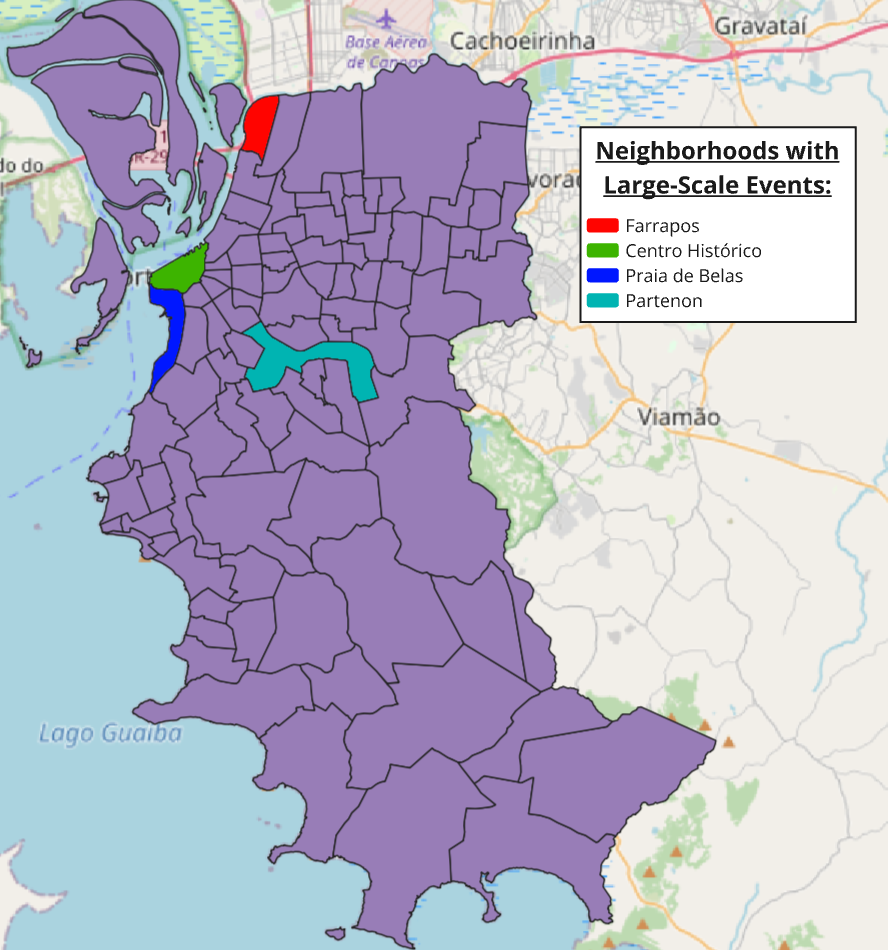
\includegraphics[width=0.70\textwidth]{fig/res-event-disruptions/CityViewNeighborhoods.png}
    \caption{Locations of the four large-scale-event destinations in the neighborhood-level representation of Porto Alegre. Events A and B occur in Farrapos and Praia de Belas, Event C in Centro Hist\'orico, and Event D in Partenon.}
    \label{fig:large_event_locations}
\end{figure}

The experiment configurations contains a no-event baseline and every combination of one, two, three, and four events. 
In these configurations, the selected events occur at 19:00. Because requests scheduled at the same step are processed sequentially, each event operates on the population distribution resulting from the requests processed before it. 
A final configuration uses the same four events but separates part of their demand over the day: Event C occurs at 09:00, Event D at 14:00, and Events A and B at 19:00.

The recorded outcome is population displacement between POIs. One displacement corresponds to one represented person moving from an origin to a destination. %These data characterize the movement generated during the simulation, but they do not separately identify unique event attendees, repeated attendance, fulfilled event demand, or unmet event demand. The results are therefore interpreted in terms of displacement rather than direct event attendance.


\subsubsection{Event Location and Concurrent Demand}
\label{sec:large_event_concurrent_demand}

Table~\ref{tbl:results_displacement} presents the aggregate displacement results for all event configurations. The no-event baseline produces 2,570,658 displacements during the simulated day, corresponding to an average of 1.8240 displacements per inhabitant.

\begin{table}[ht]
\centering
\caption{Displacement results for the large-scale-event simulations. Scenario names identify the events added to the normal-life baseline. All simulations consider the neighborhood-level environment.}
\label{tbl:results_displacement}
\begin{tabular}{@{}lrrr@{}}
\toprule
\textbf{Scenario} &
\shortstack{\textbf{Total}\\\textbf{displacements}} &
\shortstack{\textbf{Displacements}\\\textbf{per inhabitant}} &
\shortstack{\textbf{Increase over}\\\textbf{baseline}} \\
\midrule
Baseline               & 2,570,658 & 1.8240 & --- \\
\midrule
Baseline+A             & 3,290,469 & 2.3347 & 28.00\% \\
Baseline+B             & 3,300,782 & 2.3421 & 28.40\% \\
Baseline+C             & 3,289,002 & 2.3337 & 27.94\% \\
Baseline+D             & 3,281,102 & 2.3281 & 27.64\% \\
\midrule
Baseline+AB            & 3,786,856 & 2.6870 & 47.31\% \\
Baseline+AC            & 3,748,417 & 2.6597 & 45.82\% \\
Baseline+AD            & 3,804,017 & 2.6991 & 47.98\% \\
Baseline+BC            & 3,738,497 & 2.6526 & 45.43\% \\
Baseline+BD            & 3,839,126 & 2.7240 & 49.34\% \\
Baseline+CD            & 3,826,094 & 2.7148 & 48.84\% \\
\midrule
Baseline+ABC           & 4,042,413 & 2.8683 & 57.25\% \\
Baseline+ABD           & 4,109,929 & 2.9162 & 59.88\% \\
Baseline+ACD           & 4,069,223 & 2.8873 & 58.29\% \\
Baseline+BCD           & 4,081,563 & 2.8961 & 58.78\% \\
\midrule
Baseline+ABCD          & 4,235,926 & 3.0056 & 64.78\% \\
Baseline+ABCD+DiffStep & 4,638,329 & 3.2911 & 80.43\% \\
\bottomrule
\end{tabular}
\end{table}

The four single-event configurations produce similar aggregate increases in mobility. Their total displacement ranges from 3,281,102 for Event D to 3,300,782 for Event B, corresponding to increases between 27.64\% and 28.40\% relative to the baseline. Thus, under the same requested event population, the four destinations result in comparable overall movement volumes.

Their spatial distributions, however, are not identical. Figure~\ref{fig:large_event_single_displacement} compares displacement distance for the no-event baseline and each single-event scenario. Although all four events produce similar total displacement, their destinations occupy different parts of the city and consequently draw population over different spatial ranges. For example, Event A produces comparatively more displacement around the longer-distance portion of the distribution. The effect of event location is therefore more visible in the spatial distribution of movement than in its aggregate volume.

\begin{figure}[ht]
    \centering
    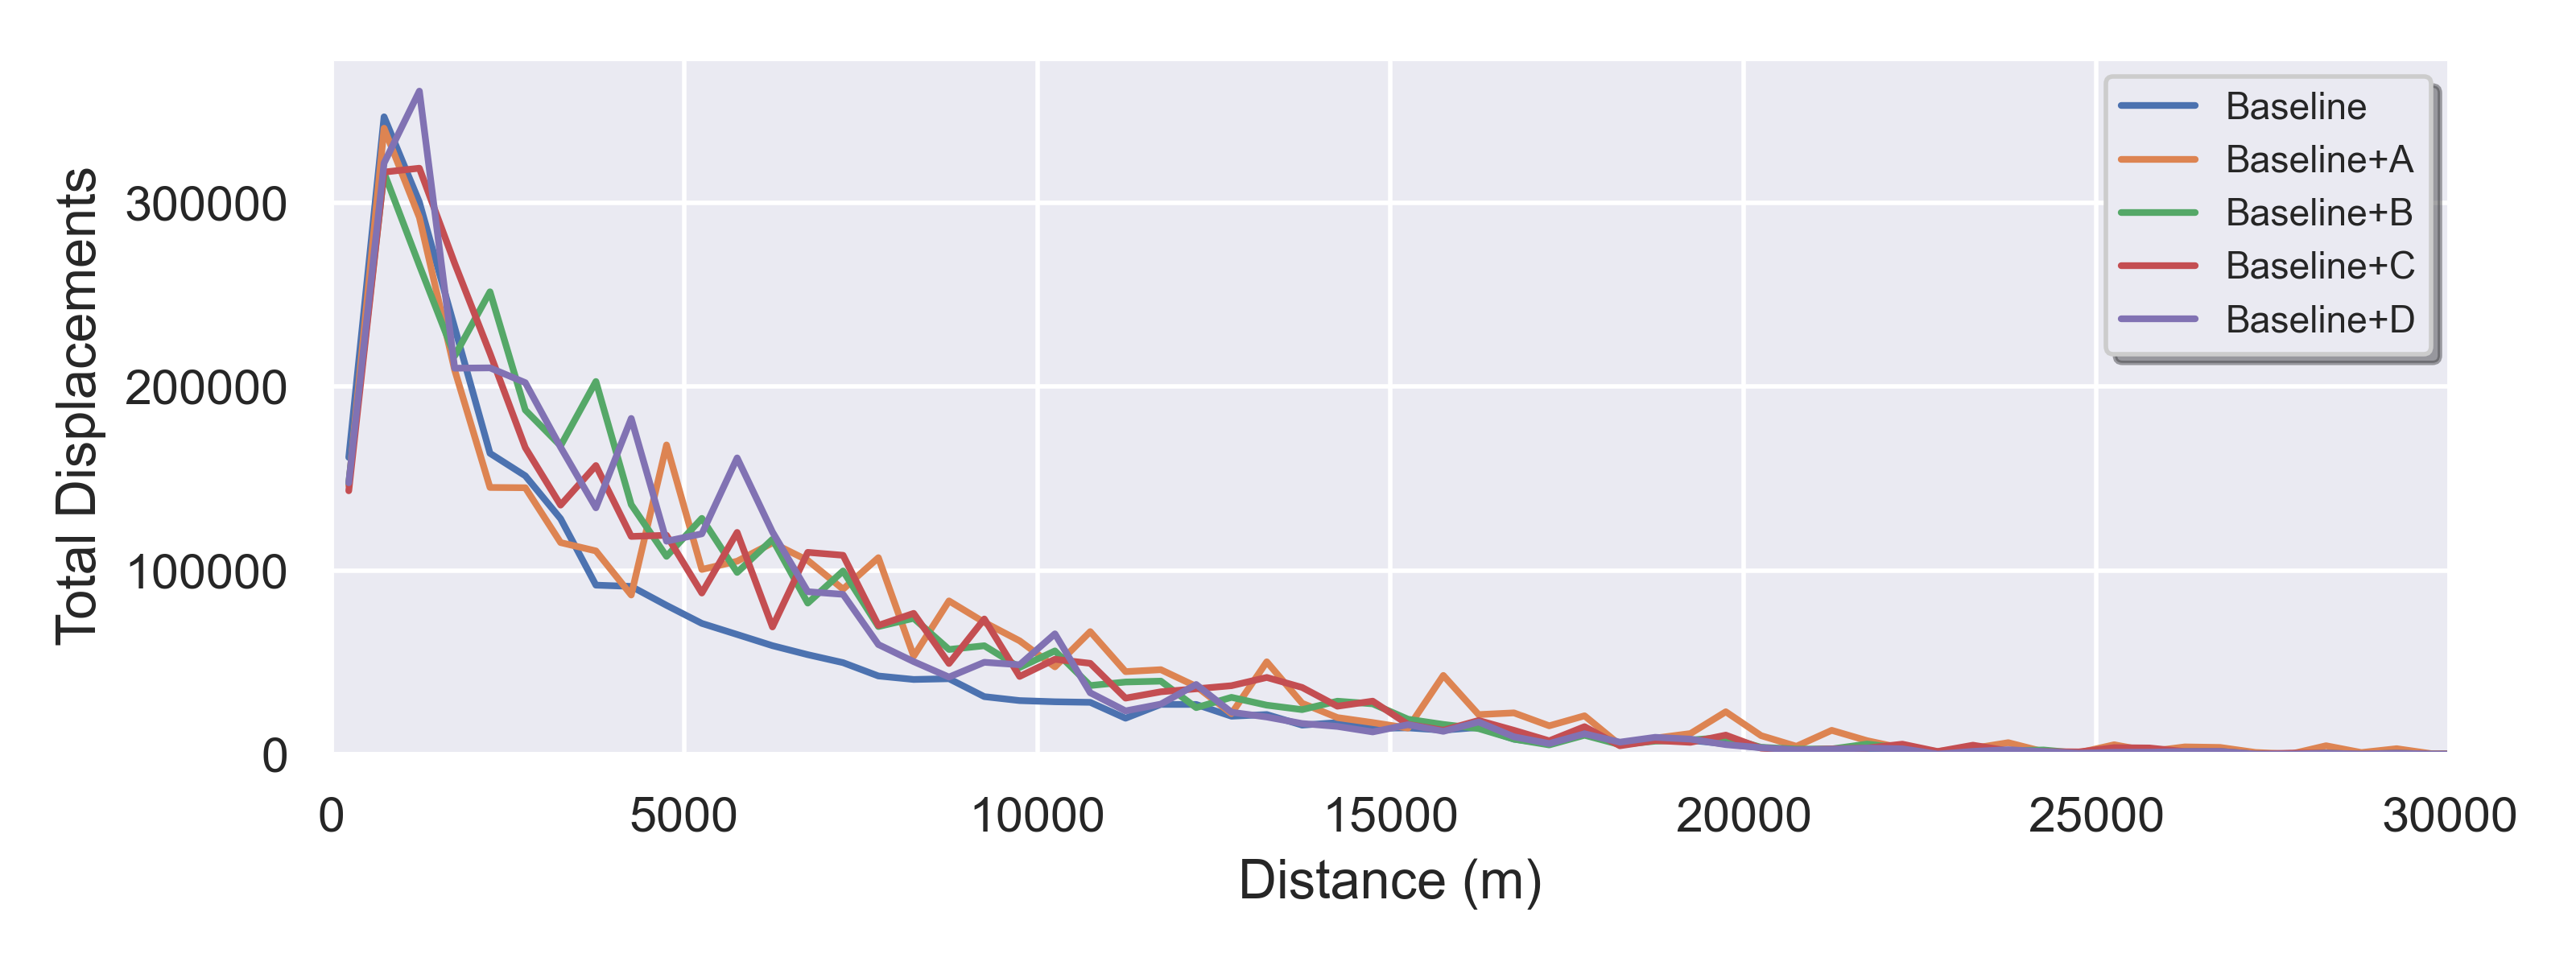
\includegraphics[width=0.98\linewidth]{fig/res-event-disruptions/Displacement_SingleEvent.png}
    \caption{Population-displacement distributions for the no-event baseline and the four single-event scenarios. Each event requests the same population quantity, while differences among the curves reflect the spatial relationship between the event destination and the population available across the city.}
    \label{fig:large_event_single_displacement}
\end{figure}

Adding further simultaneous events progressively increases total displacement. Two-event scenarios produce increases between 45.43\% and 49.34\%, while three-event scenarios produce increases between 57.25\% and 59.88\%. When all four events occur at 19:00, the simulation reaches 4,235,926 displacements, or 64.78\% above the baseline.

However, the effects of concurrent events are not additive. If the events contributed independently to displacement, the combined effect of Events A, B, and C would be expected to approximate the sum of their individual increases. Instead, while Events A, B, and C individually increase displacement by 28.00\%, 28.40\%, and 27.94\%, their simultaneous configuration produces an increase of only 57.25\%. This sub-additive behavior reflects the interaction among event requests operating on the same evolving population state.
%The increase is nevertheless non-additive. For example, Events A, B, and C individually increase displacement by 28.00\%, 28.40\%, and 27.94\%, respectively, whereas their simultaneous ABC configuration increases displacement by 57.25\%. The same pattern is visible as more concurrent events are introduced.

This behavior results from the events operating on the same evolving population state. Population participating in ordinary work and school mobility may already be located away from home when an event request is processed, and each gathering request modifies the population distribution observed by subsequent requests at the same step. Consequently, simultaneous event demands cannot be interpreted as independent additions to the normal-life baseline.

The resulting non-additivity is evidence of interaction among concurrent population demands, but it should not be interpreted as a direct measurement of event-attendance fulfillment. The preserved results do not record the requested and fulfilled attendance of each event separately.


\subsubsection{Event Timing}
\label{sec:large_event_timing}

The final comparison examines how the timing of Events A, B, C, and D affects population displacement, comparing a configuration in which all four events occur simultaneously with one in which their demands are distributed throughout the day.
%The final comparison examines the temporal distribution of the same four event demands. 
Figure~\ref{fig:large_event_timing_displacement} compares the baseline with the four-event simultaneous configuration and the condition in which Events C and D occur earlier in the day.

\begin{figure}[ht]
    \centering
    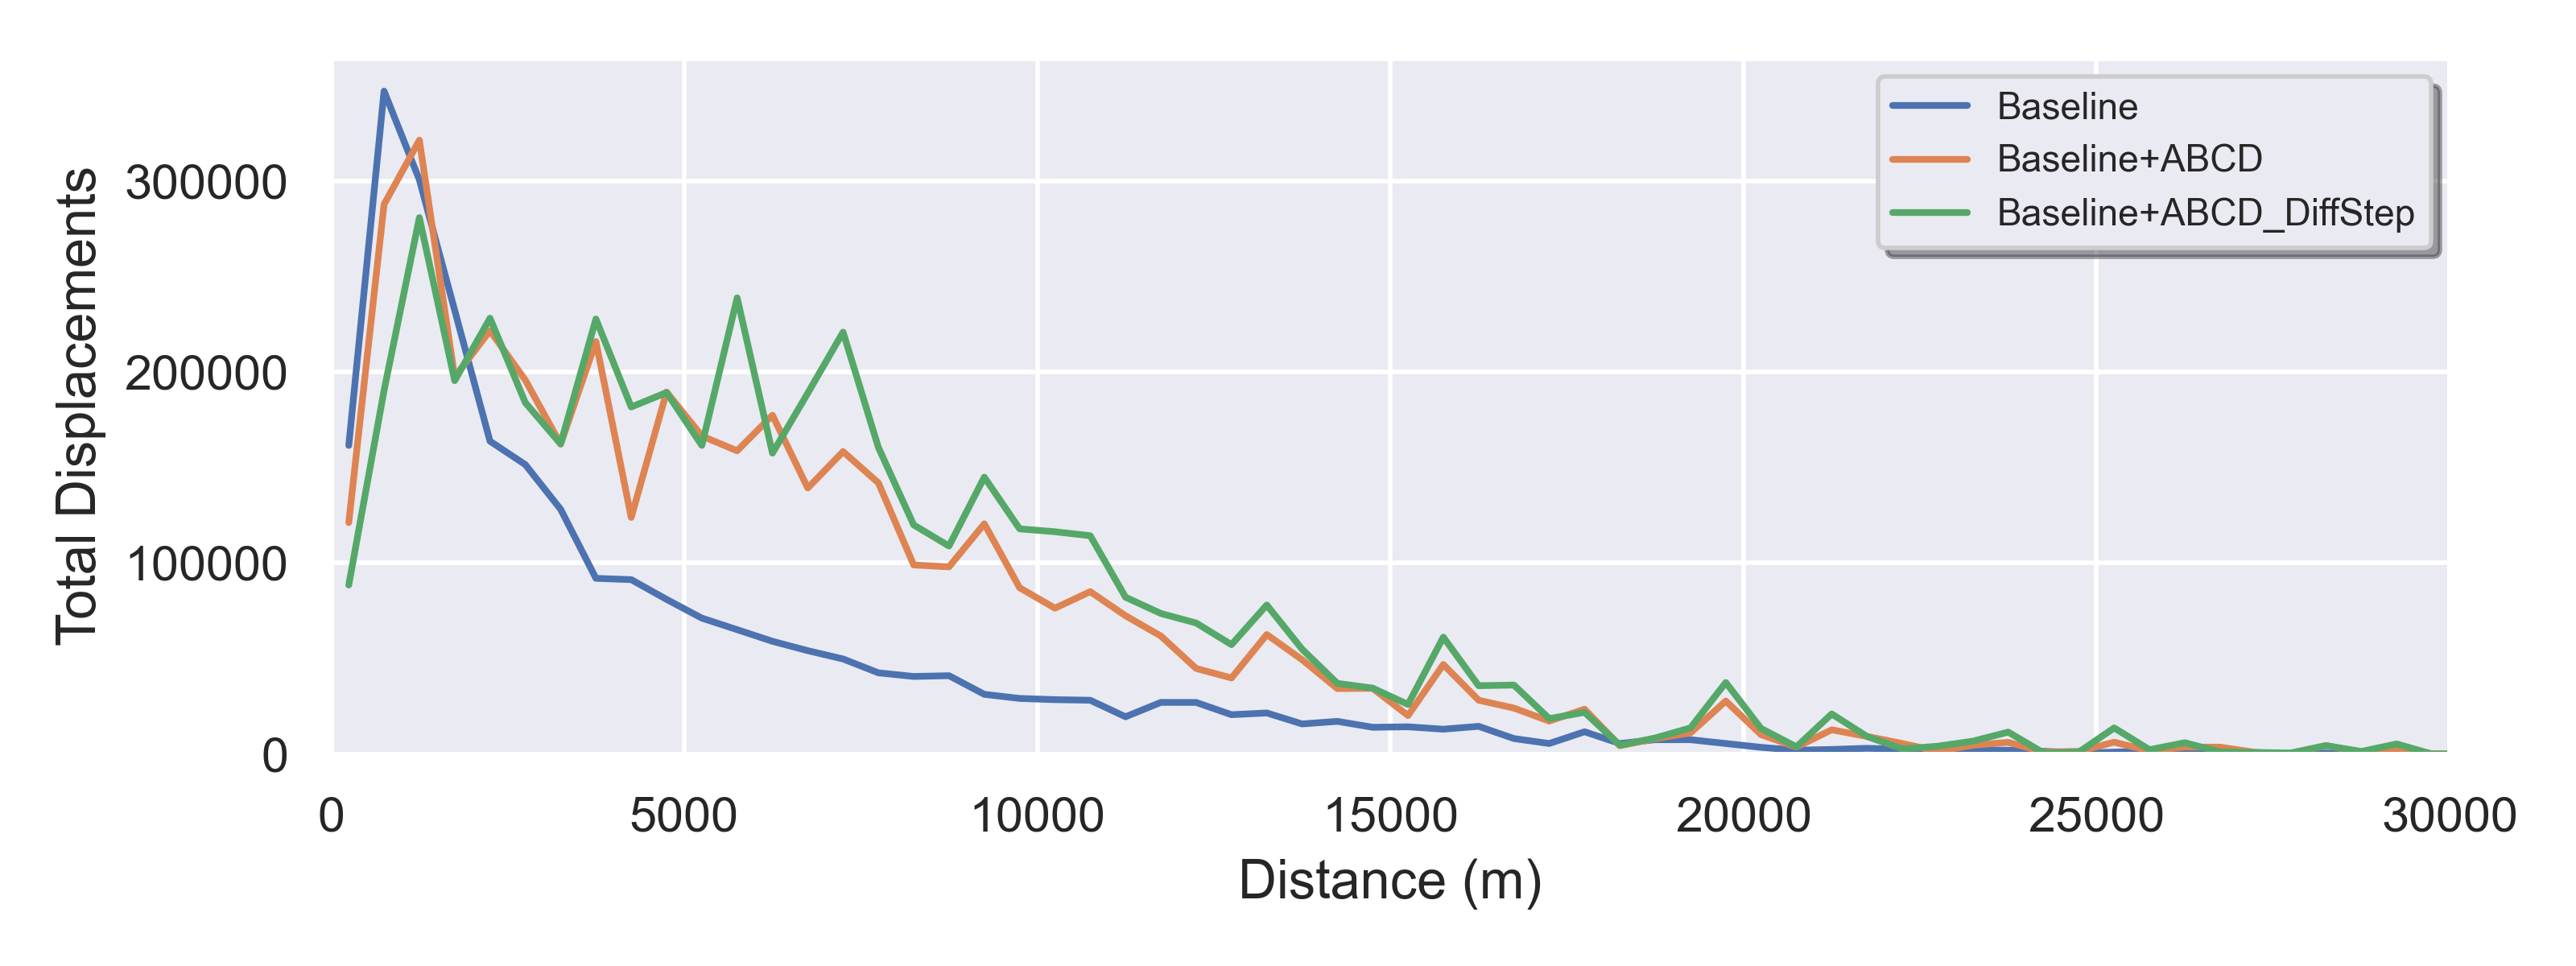
\includegraphics[width=0.98\linewidth]{fig/res-event-disruptions/Displacement_AllEvents.png}
    \caption{Population-displacement distributions for the no-event baseline, four events occurring simultaneously at 19:00, and the staggered four-event configuration in which Event C occurs at 09:00, Event D at 14:00, and Events A and B at 19:00.}
    \label{fig:large_event_timing_displacement}
\end{figure}

With all four events occurring simultaneously, total displacement reaches 4,235,926, corresponding to 3.0056 displacements per inhabitant and an increase of 64.78\% over the no-event baseline. When Events C and D occur earlier, total displacement increases to 4,638,329, or 3.2911 displacements per inhabitant. This represents an 80.43\% increase over baseline and 402,403 additional displacements relative to the simultaneous four-event configuration.

The difference shows that exceptional demand is affected by when it is introduced, not only by its total requested quantity. When four requests are concentrated at the same step, they operate sequentially on the population available at that moment. Separating part of this demand over the day allows the population distribution to evolve between requests, so population relocated earlier may subsequently become available for other movements or later gathering requests.

Overall, the large-scale-event experiments show that exceptional gathering demand affects both the volume and spatial distribution of population mobility. Event destinations with the same requested population produce similar aggregate displacement but different distance distributions. Increasing the number of simultaneous events raises total movement, although the resulting effect is not additive because the requests interact through a shared and changing population state. Finally, distributing the same four event demands over different times produces more displacement than concentrating them at a single simulation step. These results establish the effects of exceptional demand before the following experiments consider a different departure from normal-life mobility: environmental conditions that make locations temporarily unavailable.


\subsection{Flood-Induced Mobility Disruption}
\label{sec:results_flood_mobility}

The large-scale-event experiments introduce additional demand while leaving the underlying environment available. Flooding produces a different departure from normal-life mobility by making some of the locations used by recurring activities and commutes temporarily unavailable. The experiments in this subsection examine how this disruption affects activity visits and work or school attendance, and whether activity demand can be preserved by redirecting visits toward alternative destinations.

The experiments use the reduced and complete census-sector environments introduced in Section~\ref{sec:census_sector_environments}. The reduced environment comprises 13 regions, 2,610 POIs, and a population of 159,886, while the complete environment comprises 94 regions, 16,266 POIs, and a population of 1,331,414. Each simulation covers 56 days with 24 hourly steps per day and applies the time-varying water-level series described in Section~\ref{sec:water_level_plugin_inputs}.

Three types of comparisons are considered. First, activity scenarios expose homes, activity destinations, or both to flooding and measure the resulting fulfillment of visits to marketplaces, restaurants, and pharmacies. Second, attendance-controlled commute scenarios additionally expose work and school destinations, allowing the effects on recurring work and school mobility to be measured. Finally, an adaptation scenario allows unavailable activity destinations to be replaced by the nearest available POI of the same type. Work and school destinations remain non-substitutable under the evaluated configuration.


\subsubsection{Environmental Exposure and Mobility Loss}
\label{sec:flood_environmental_exposure}

The applied water-level series changes the number and spatial distribution of POIs available throughout the 56-day simulation. Figure~\ref{fig:environment_disruption_flood_exposure} presents the simulated water-level sequence together with the POI availability state at its maximum value of 5.33~m.

At this maximum level, 513 of the 2,610 POIs in the reduced environment and 1,920 of the 16,266 POIs in the complete environment are unavailable. The affected locations include homes, activity destinations, workplaces, and schools, creating periods in which recurring mobility can no longer be executed under the same conditions as the normal-life baseline.

%SO: acrescentei abaixo
%GA: certo
As a plausibility reference, the maximum water level considered in this experiment (5.33 m) corresponds to the historical peak reported for the Guaíba during the May 2024 flood, reached on May 5 and 6. During this event, 157,701 people were reported as affected in Porto Alegre, corresponding to 11.8\% of the city’s population.\footnote{CNN Brasil, “Enchente afetou quase 12\% da população de Porto Alegre; veja números sobre o impacto da chuva na cidade,” May 16, 2024. Available at: \url{https://www.cnnbrasil.com.br/nacional/enchente-afetou-quase-12-da-populacao-de-porto-alegre-veja-numeros-sobre-o-impacto-da-chuva-na-cidade/}}. At the same maximum water level, 1,920 of the 16,266 POIs in the complete simulated environment are unavailable, also corresponding to approximately 11.8\%. Although the percentage of unavailable POIs and the percentage of affected population represent different quantities and are therefore not directly comparable, their similar order of magnitude provides a useful contextual reference for the scale of environmental exposure represented in the experiment. This comparison is intended as a plausibility reference rather than as an empirical validation of the simulated flood impacts.


\begin{figure}[ht]
    \centering
    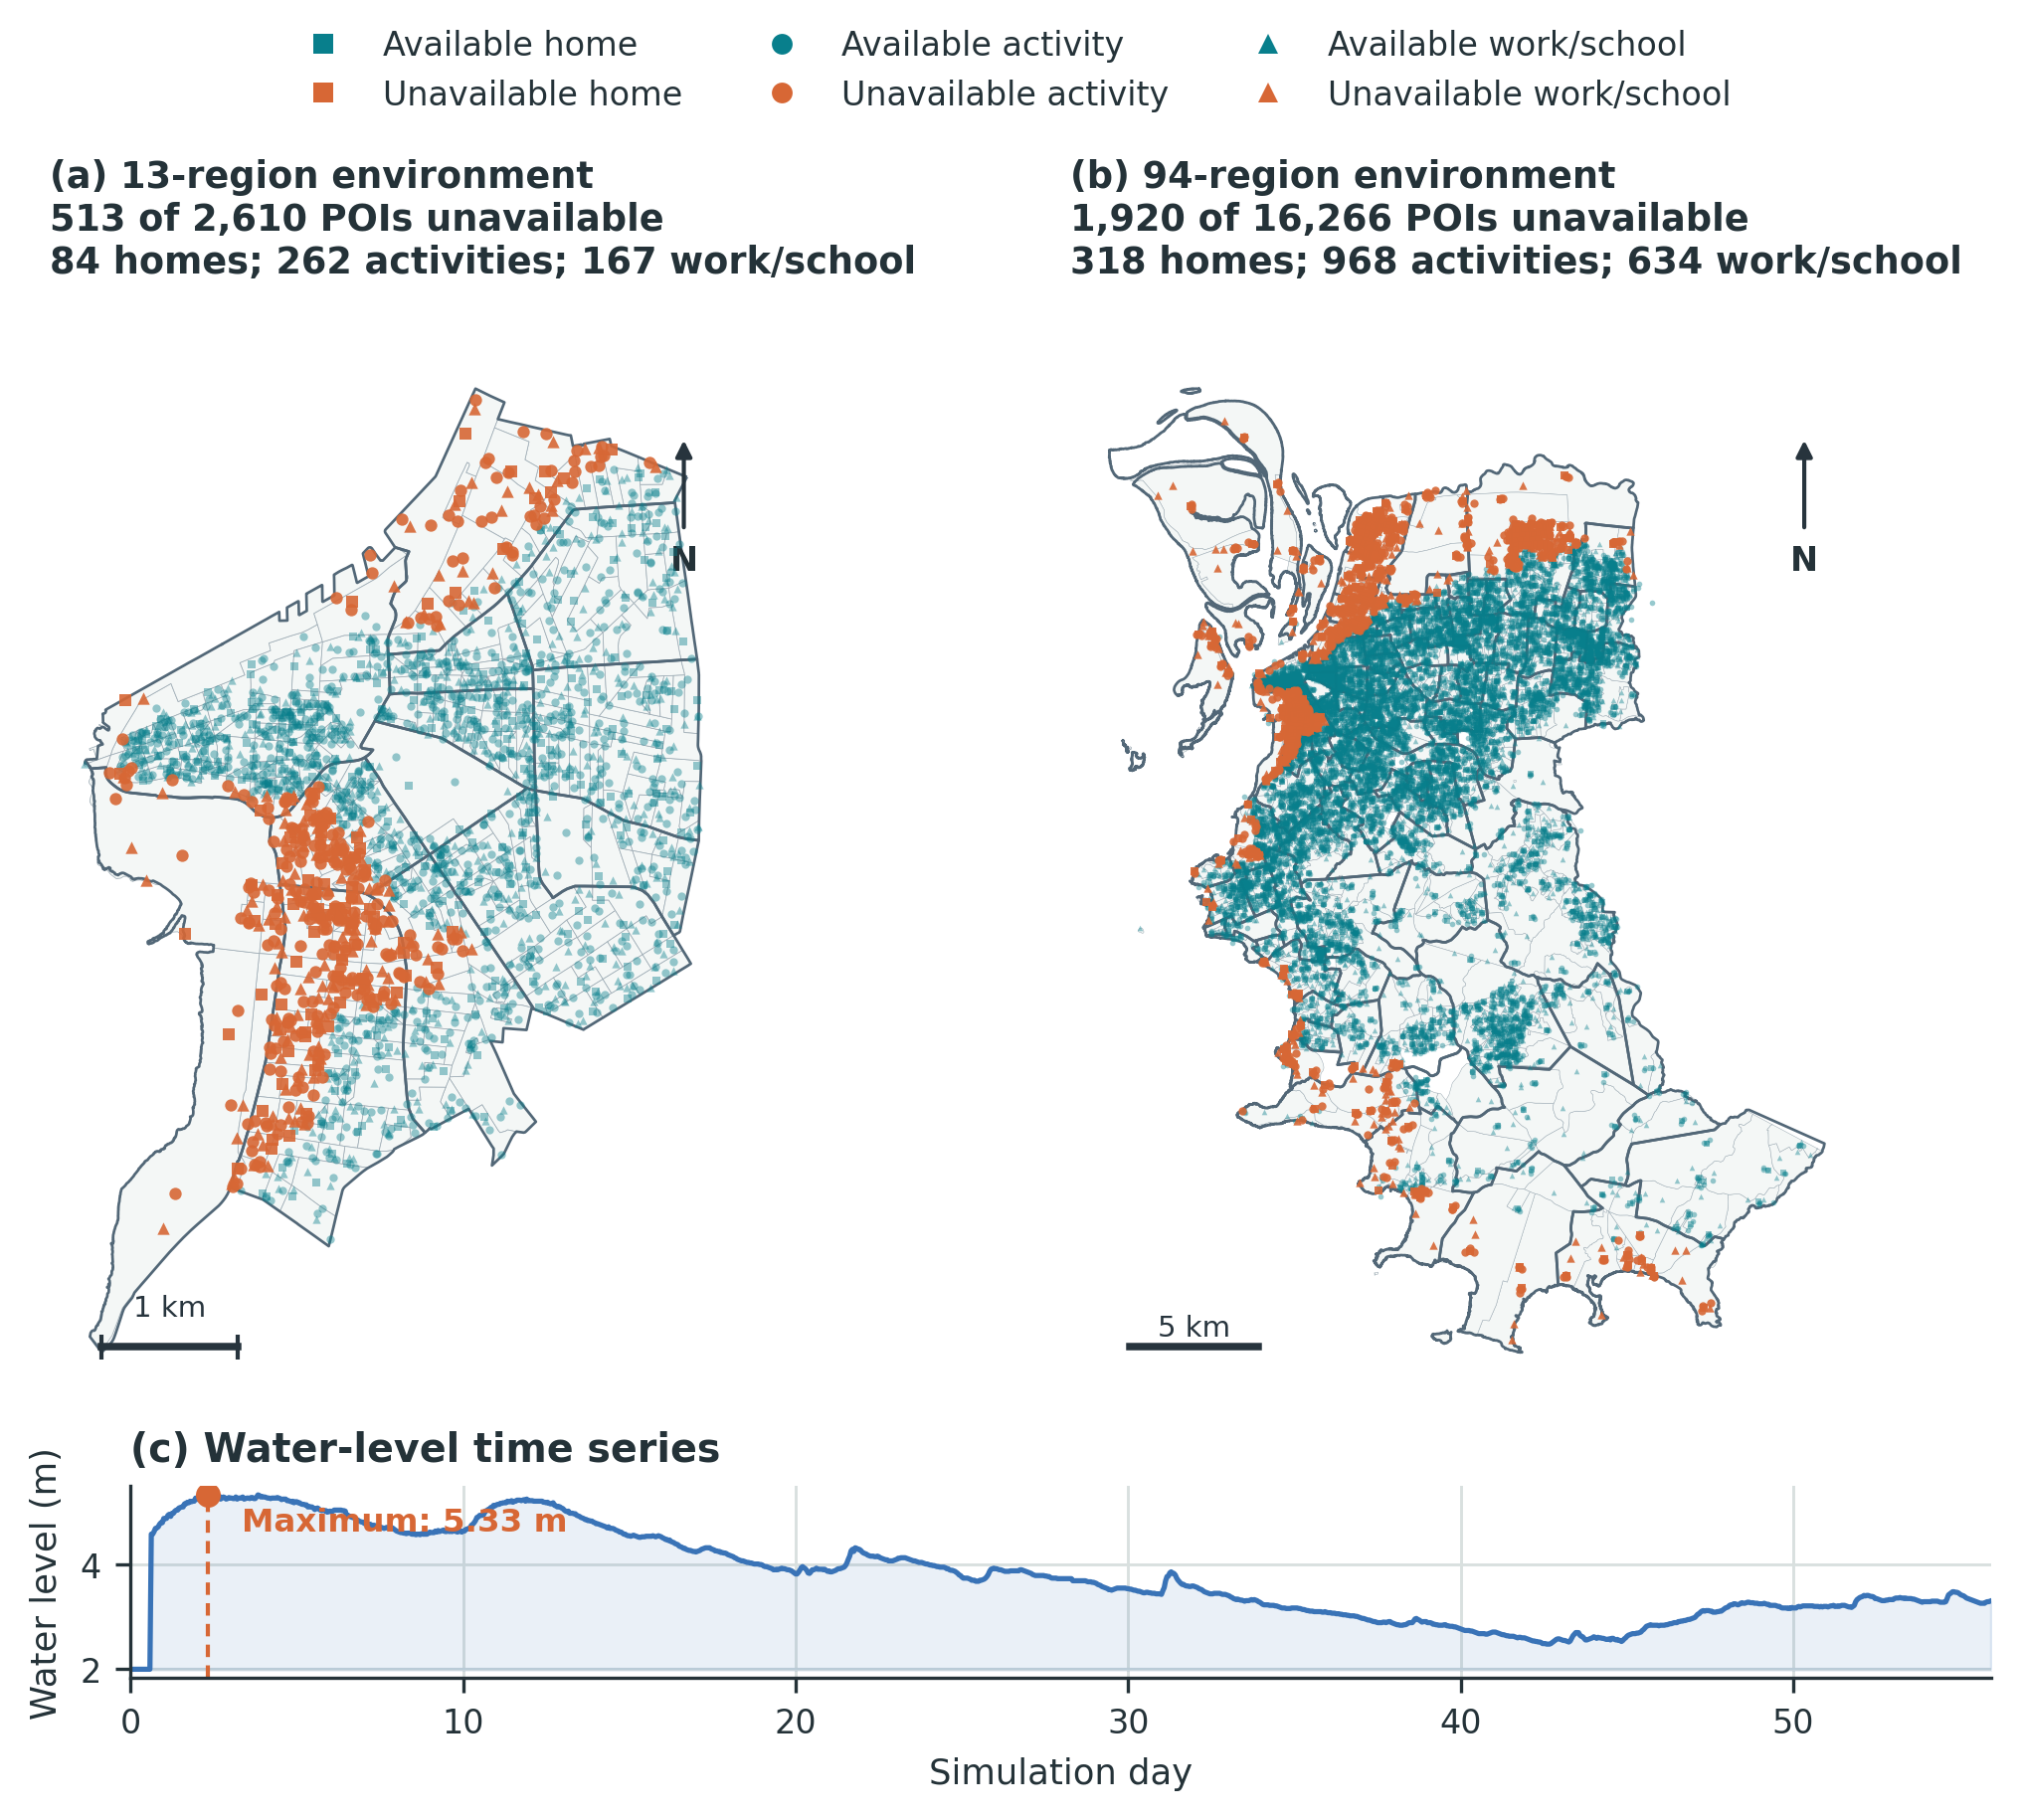
\includegraphics[width=\linewidth]{fig/res-event-disruptions/environment_disruption_flood_exposure.png}
    \caption{POI availability under the simulated flood conditions. Panels (a) and (b) show available and unavailable POIs at the maximum simulated water level of 5.33~m in the reduced and complete census-sector environments, respectively. Panel (c) presents the water-level series applied throughout the 56-day simulation.}
    \label{fig:environment_disruption_flood_exposure}
\end{figure}

The resulting mobility loss depends on whether flooding affects an origin or a requested destination. Figure~\ref{fig:flood_fulfillment_comparison} summarizes activity and commute fulfillment under the different exposure conditions.

%GA: poderia ser uma tabela. Se manter figura, ajustar o inicio do eixo X
\begin{figure}[ht]
    \centering
    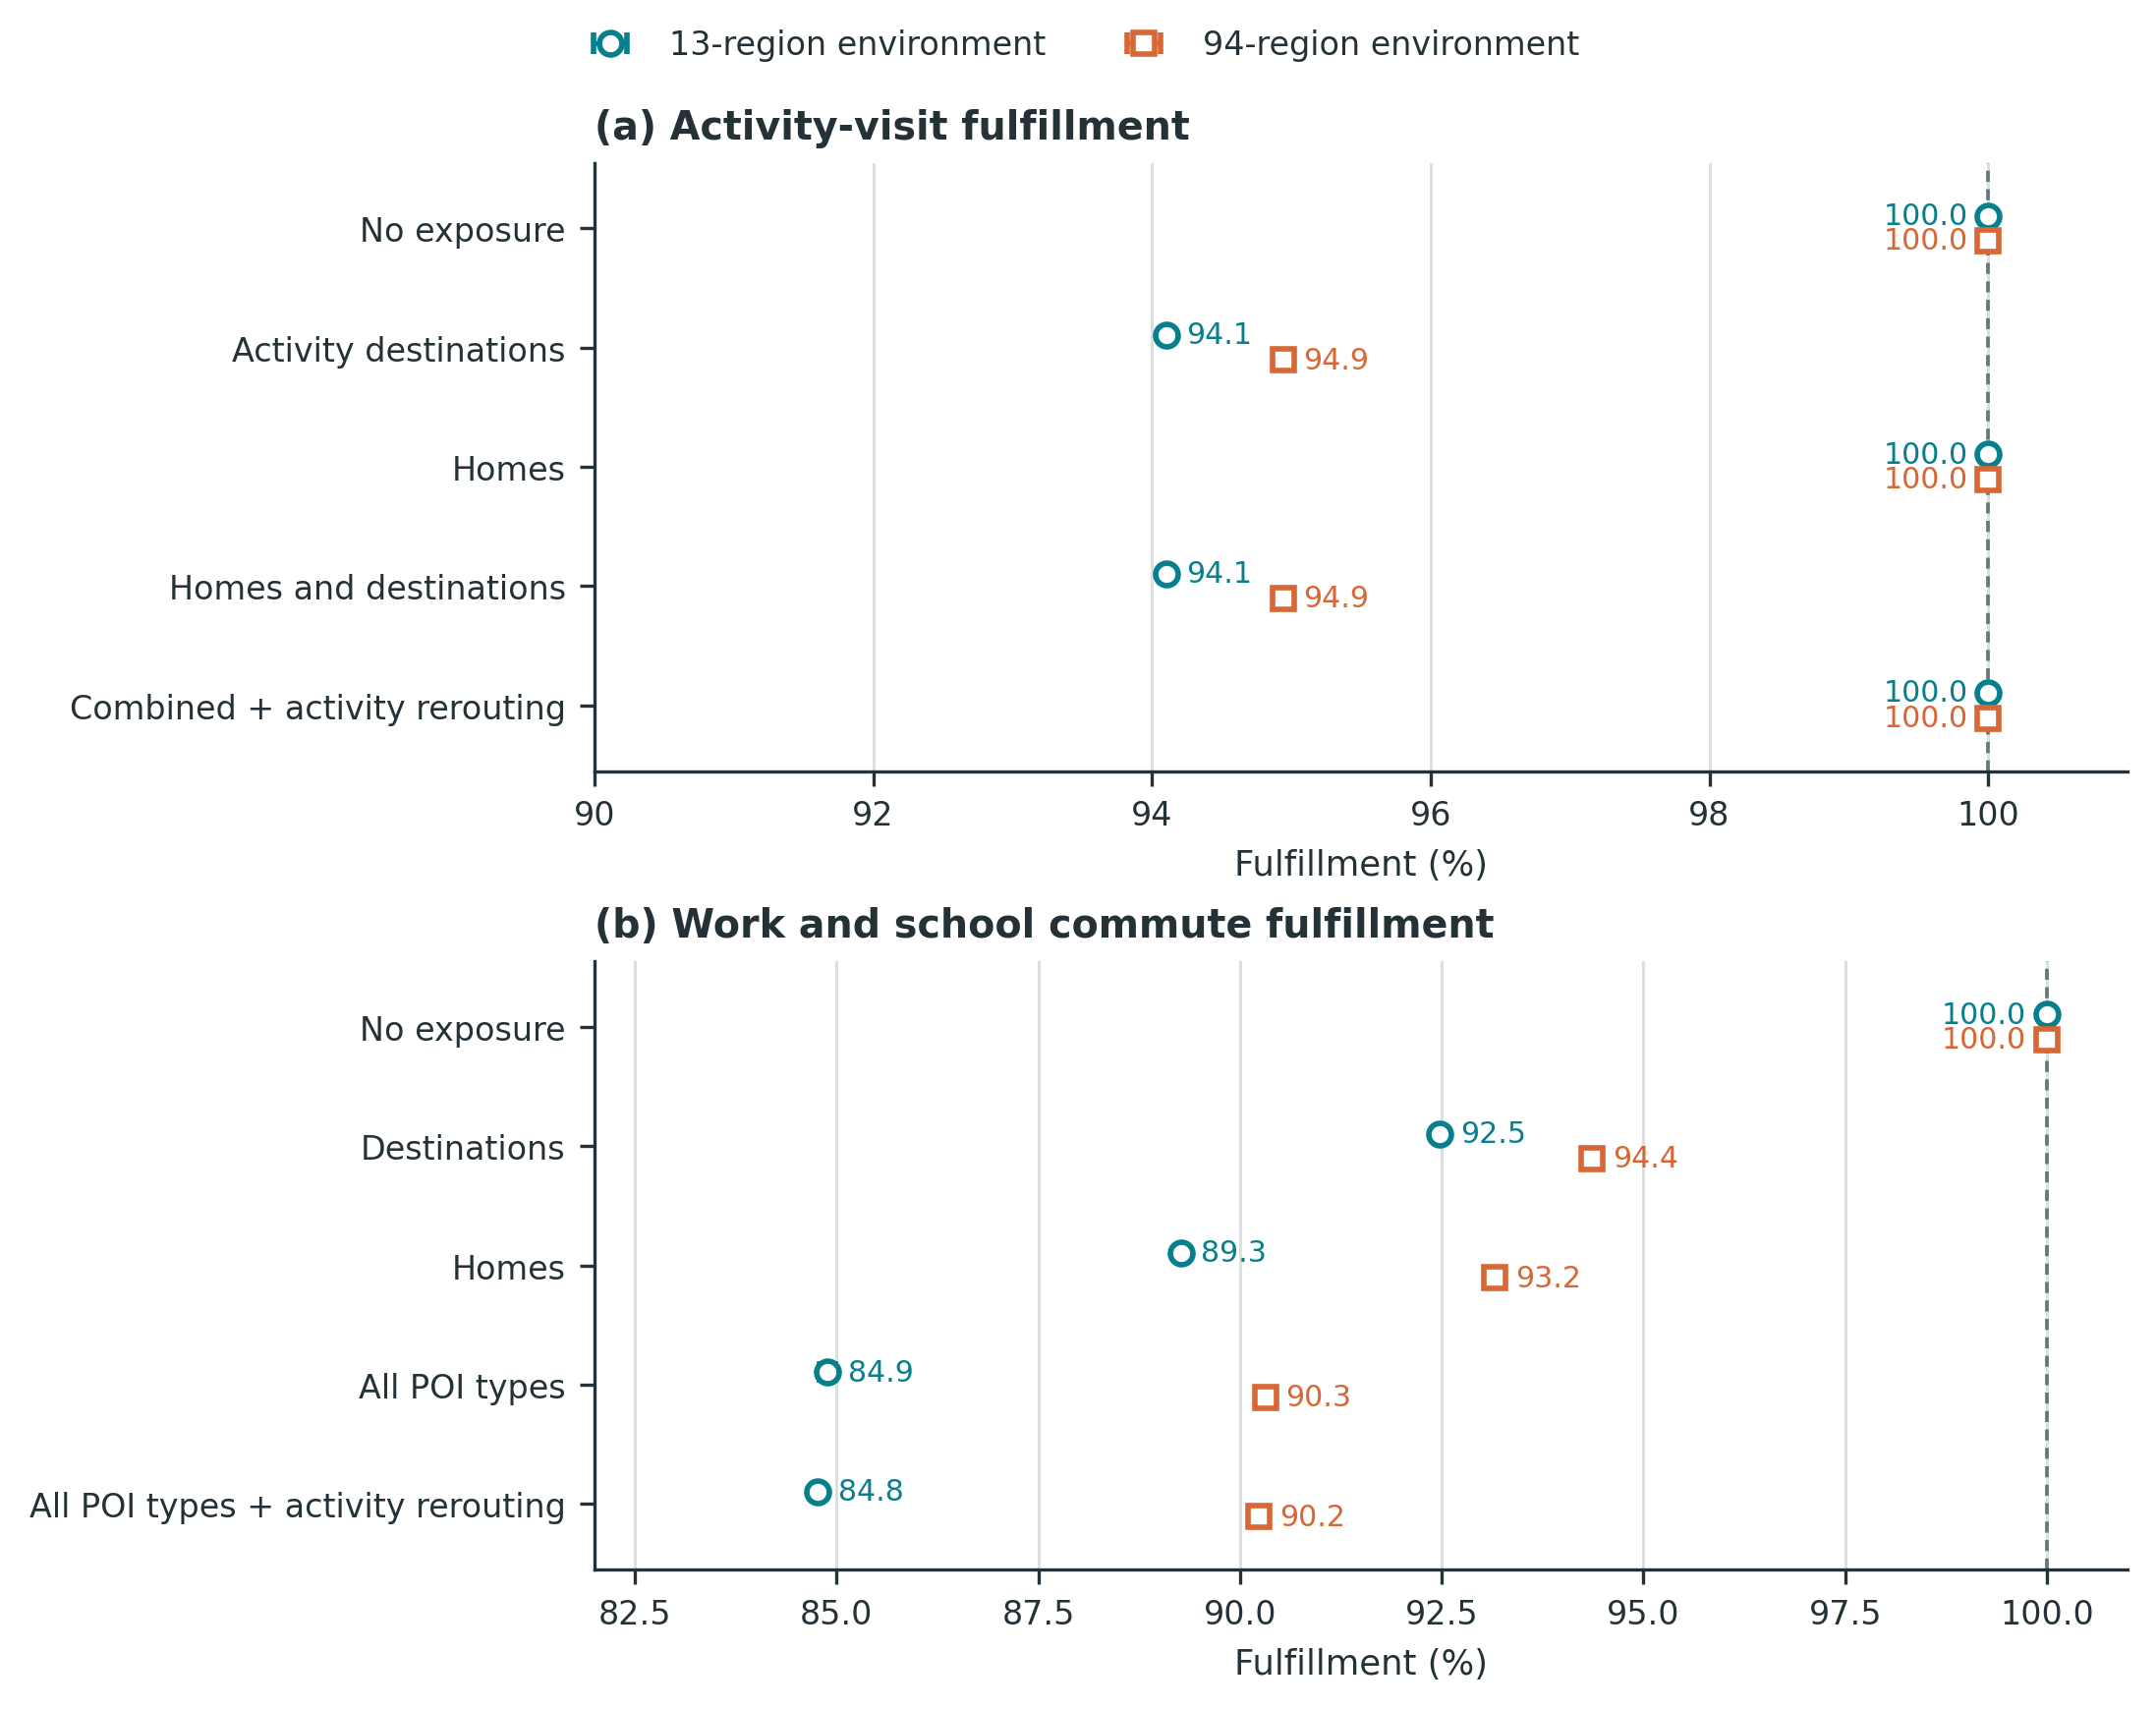
\includegraphics[width=\linewidth]{fig/res-event-disruptions/environment_disruption_fulfillment_comparison.png}
    \caption{Mobility fulfillment under the evaluated flood conditions in the reduced and complete census-sector environments. Panel (a) shows activity-visit fulfillment and panel (b) shows the combined fulfillment of work and school commutes. Results compare the normal-life reference with unavailable destinations, unavailable homes, combined exposure, and combined exposure with activity-destination substitution. Points are means over five simulation runs.}
    \label{fig:flood_fulfillment_comparison}
\end{figure}

For activity visits, unavailable destinations are the main source of lost demand. In the reduced environment, activity fulfillment decreases from 100\% under the reference condition to 94.10\% when marketplaces, restaurants, and pharmacies are exposed, corresponding to 169,736 unmet visits over the 56-day simulation. Exposing homes alone does not reduce activity fulfillment, and exposing homes and destinations together produces the same 94.10\% fulfillment as destination exposure alone.

The complete environment presents the same general pattern. Activity-destination exposure reduces fulfillment from approximately 100\% to 94.94\%, leaving approximately 1.21 million visits unmet. Home exposure alone has negligible effect on the number of fulfilled visits, while combined home and destination exposure again produces approximately the same activity loss as destination exposure.

These results indicate that the activity configuration can compensate for unavailable population sources by drawing eligible population from other available homes. It cannot, however, complete a requested visit when its activity destination is unavailable unless destination substitution is enabled.

Work and school commutes are affected differently because both the population origin and the requested destination are required for attendance. In the reduced environment, commute fulfillment decreases from effectively 100\% under normal-life conditions to 92.47\% when destinations are exposed and to 89.27\% when homes are exposed. When all relevant POI types are exposed, fulfillment falls further to 84.89\%.

The same pattern occurs in the complete environment, although the reduction is smaller. Destination exposure results in 94.36\% commute fulfillment, home exposure in 93.16\%, and combined exposure in 90.31\%. Thus, flooding both origins and destinations produces the largest disruption in both spatial representations.

Under combined exposure, student fulfillment remains slightly higher than worker fulfillment. In the reduced environment, the respective means are 86.30\% and 84.33\%, a difference of 1.96 percentage points. In the complete environment, the respective means are 90.66\% and 90.18\%, a difference of 0.49 percentage points. %Because this separation is modest, particularly in the complete environment, Figure~\ref{fig:flood_fulfillment_comparison} retains the aggregate commute result.

Unlike the activity results, where unavailable homes can largely be compensated by alternative population sources, commute demand is tied to the population's home and requested work or school destination. As a result, unavailable origins as well as unavailable destinations contribute directly to unmet attendance.

Completed-trip distance is not emphasized as a primary disruption measure. In several flooded conditions, the mean distance among completed movements decreases because some trips are suppressed entirely. Such changes therefore describe the subset of movements that remain feasible rather than an improvement in accessibility.


\subsubsection{Activity-Destination Adaptation}
\label{sec:flood_destination_adaptation}

The final flood-mobility comparison examines whether activity demand lost through unavailable destinations can instead be redirected toward alternative locations. Under this configuration, a visit whose requested marketplace, restaurant, or pharmacy is unavailable is assigned to the nearest available POI of the same type. The requested and receiving destinations remain distinguishable in the results, allowing the amount of recovered demand and the additional spatial burden of substitution to be measured. %GA: burden foi o termo sugerido para "carga" adicional (população extra que os POIs recebem quando demanda é redirecionada)

In the reduced environment, substitution restores all 169,736 activity visits that would otherwise be suppressed by destination unavailability. In the complete environment, it restores essentially all of the approximately 1.21 million affected visits, leaving only about five unmet requests per run. Activity fulfillment therefore returns to approximately 100\% in both environments.

This recovery is accompanied by additional displacement between the requested and receiving destinations. Rerouted visits travel an average of approximately 294~m beyond their requested destination in the reduced environment and 1.17~km in the complete environment. Figure~\ref{fig:flood_rerouting_burden} summarizes this trade-off together with the redistribution of demand among receiving POIs.

%GA: também poderia ser uma tabela
\begin{figure}[ht]
    \centering
    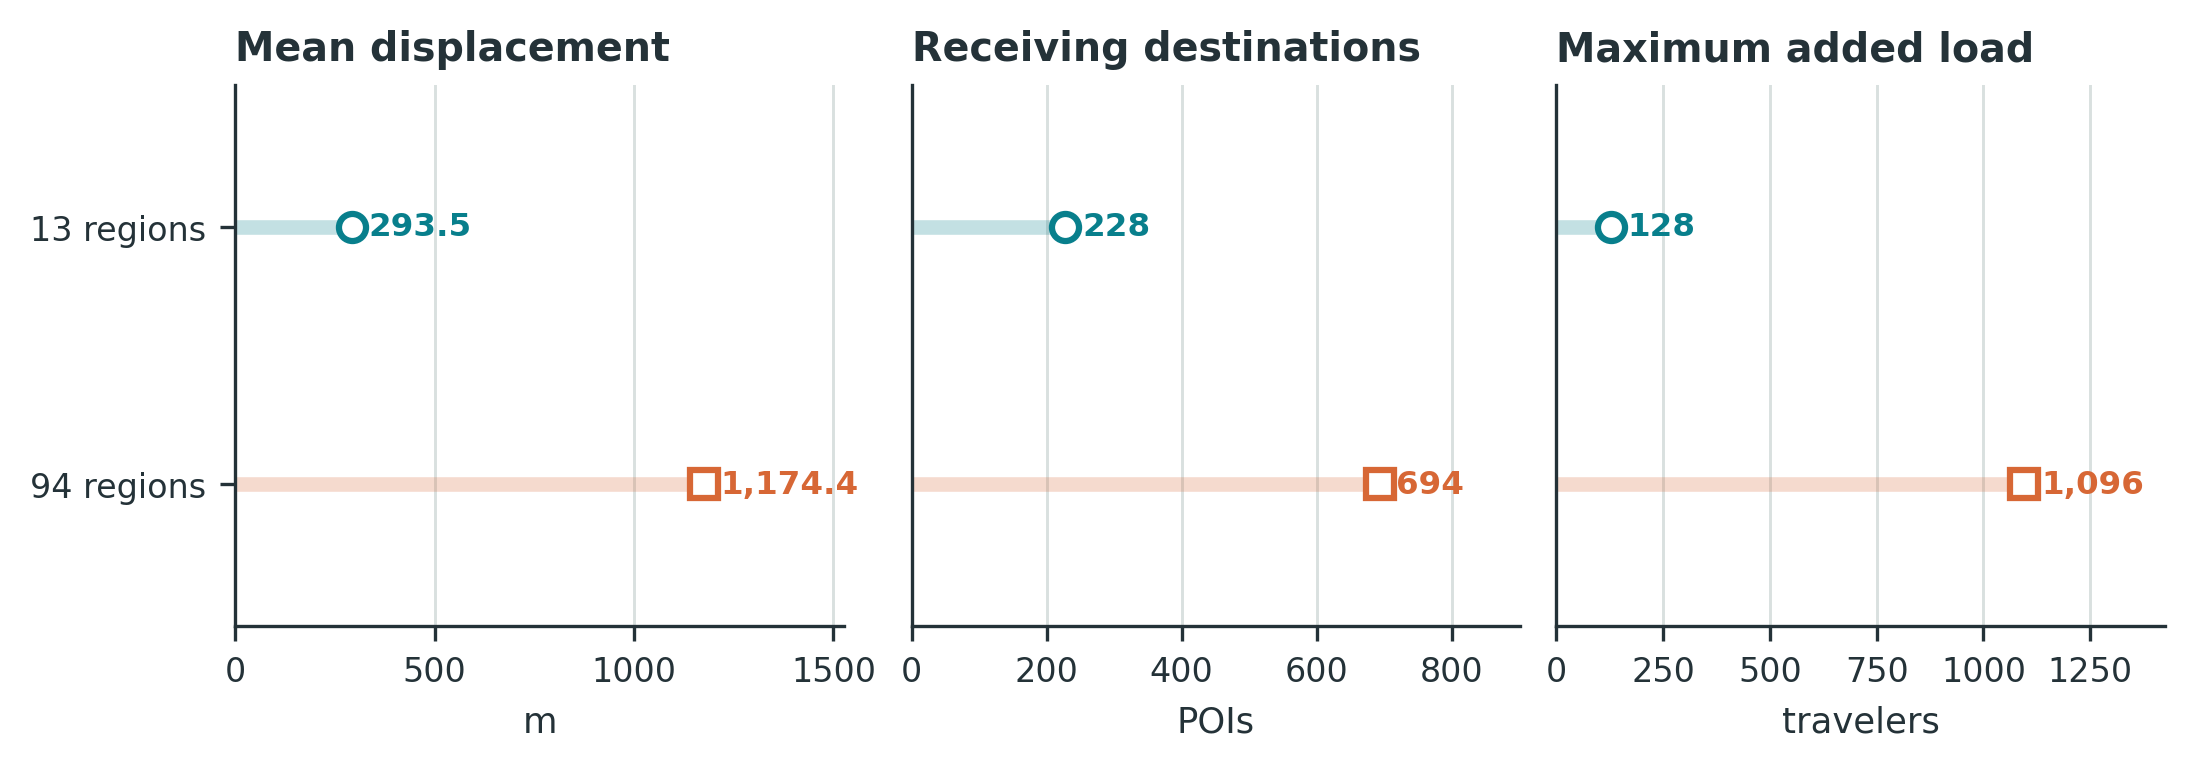
\includegraphics[width=\linewidth]{fig/res-event-disruptions/environment_disruption_rerouting_burden.png}
    \caption{Activity-destination adaptation under combined home and destination exposure to flood. The panel on the left shows the mean displacement between requested and receiving destinations, the panel in the center shows the number of distinct receiving activity POIs, and the panel on the right shows the peak rerouted-only concurrent population at one receiving POI, excluding direct demand. Values are means over five simulation runs for the reduced and complete census-sector environments.}
    \label{fig:flood_rerouting_burden}
\end{figure}

%SO: re-escrevi porque achei confuso, e acho que falta o total -- 228 de quantas???
%GA: adicionei os totais
Under the activity-destination substitution configuration, the demand redirected from unavailable destinations is distributed among 228 of the 1,305 activity POIs in the reduced environment and 694 of the 8,133 in the complete environment.
%The redirected demand is distributed among 228 receiving activity POIs in the reduced environment and 694 in the complete environment. 
The largest additional concurrent concentration attributable to rerouted population reaches 128 people at one receiving POI in the reduced environment and 1,096 in the complete environment.

These values do not represent facility-capacity violations, since activity destinations are not assigned service capacities in this experiment. Instead, they characterize how the nearest-available substitution policy redistributes demand when the originally requested locations cannot be used. The complete environment requires substantially greater displacement and produces larger concentrations of redirected population under the same adaptation rule.

Importantly, this adaptation applies only to activity destinations. Workplaces and schools remain associated with their originally requested destinations. Consequently, restoring activity demand does not restore commute fulfillment. Under combined exposure, commute fulfillment remains approximately 84.8\% in the reduced environment and 90.2\% in the complete environment whether activity substitution is enabled or not.

The flood experiments therefore show two distinct responses to unavailable urban locations. Without adaptation, flooding suppresses recurring movement, with the largest commute losses occurring when both origins and destinations are affected. Allowing substitution can preserve almost all activity demand, but transfers part of the disruption into additional travel and greater demand at alternative destinations. Work and school attendance remains constrained because these destinations are not treated as interchangeable.

These results provide a complementary view of exceptional mobility to the large-scale-event experiments. Large-scale events add demand to an otherwise available environment, whereas flooding removes some of the locations required by normal-life movement. The shelter experiments considered next extend this disruption further by introducing new protection-seeking movement toward a capacity-constrained network of facilities.


\subsection{Evacuation and Shelter Response}
\label{sec:results_shelter_response}

The preceding experiments examined two departures from normal-life mobility: large-scale events, which introduce additional movement toward exceptional destinations, and flooding, which disrupts recurring activities and commutes by making some locations temporarily unavailable. 
Environmental disruptions may also generate new movement in response to population exposure. The shelter experiments examine this additional response by representing populations affected by flooding and evaluating their relocation toward a spatially distributed and capacity-constrained shelter network.

The experiments use the neighborhood-level environment, comprising 94 regions, 504 base POIs, and a population of 1,409,351. 
The 104 shelter POIs described in Section~\ref{sec:shelter_plugin_inputs} are added to this environment, resulting in 608 POIs. These POIs are derived from the recorded locations and capacities of shelters operating in Porto Alegre on May 15, 2024, using the real-world data source documented in that section
%SO: talvez fosse legal citar que tiveram a ver com as localizações reais dos shelters
%GA: a section de shelter já indica que são dados reais, mas também ajustei aqui.
The resulting shelter network provides a total recorded capacity of 12,519 people and has a configured initial occupancy of 10,963.
Population exposure is based on a fixed 5.30~m flood condition. After mapping the exposure data to the represented population, 182,936 people are classified as exposed and constitute the reference population used in the shelter analysis.

Each experiment covers 14 simulated days with 24 hourly steps per day. Under the reference configuration, 1\% of the exposed population is requested to evacuate per day. Evacuation requests occur at 07:00, admission to shelters is evaluated at 08:00, optional waitlist reallocation occurs at 09:00, and populations moved during reallocation are reconsidered for admission at 10:00.

The evaluated scenarios vary five aspects of this reference configuration: waitlist reallocation, daily response rate, exposure magnitude, shelter capacity, and shelter availability. Table~\ref{tbl:shelter_scenarios} summarizes the corresponding scenario groups. Each configuration is evaluated over five simulation runs. Reported values are means across these runs.%; variability is generally small and is shown in the corresponding figures where applicable.

\begin{table}[ht]
\centering
\footnotesize
\caption{Shelter scenarios and their principal comparisons.}
\label{tbl:shelter_scenarios}
\begin{tabularx}{\linewidth}{@{}p{3.1cm}p{3.0cm}X@{}}
\toprule
\textbf{Scenario group} &
\textbf{Configurations} &
\textbf{Principal comparison} \\
\midrule

Reallocation
& Off; on
& Whether redistributing waiting populations reduces congestion or improves the use of remaining shelter capacity. \\

Daily response rate
& 0.5\%, 1\%, 2\%, 5\%
& Whether introducing evacuation demand more rapidly increases protection or primarily increases congestion. \\

Exposure magnitude
& 0.25$\times$, 0.5$\times$, 1$\times$
& How changes in exposed population affect unresolved demand under fixed shelter capacity. \\

Shelter capacity
& 0.5$\times$, 1$\times$, 2$\times$, 5$\times$, 15$\times$
& At what point increasing accommodation ceases to improve protection within the 14-day simulation. \\

Shelter failure
& Largest shelter disabled; highest-capacity shelters disabled
& How loss of accommodation affects protection and whether reallocation mitigates the resulting congestion. \\

\bottomrule
\end{tabularx}
\end{table}

The analysis distinguishes final protection from congestion. Shelter coverage is defined as the final population with a \texttt{sheltered} status divided by the 182,936 mapped exposed population. Because this value includes the configured initial occupancy, it should not be interpreted as the number of people newly admitted during the simulation. Unresolved demand corresponds to the population remaining in the \texttt{in\_danger} state, while peak waitlist and accumulated waiting-person-hours characterize congestion.

Under the reference configuration, 1,556 people are newly admitted after the simulation begins. Together with the initial occupancy of 10,963, this produces a final sheltered population of 12,519, equal to the available reference capacity. Distinguishing these quantities is important: final coverage describes the shelter occupancy achieved at the end of the scenario, whereas new admissions describe the additional protection provided during the simulated evacuation period.


\subsubsection{Reference Evacuation and Reallocation}
\label{sec:shelter_reference_reallocation}

The reference experiment establishes how evacuation demand develops under the recorded shelter capacity. Table~\ref{tbl:shelter_reference_results} compares the same scenario with waitlist reallocation disabled and enabled. Accumulated waiting last column in the table) is measured in person-hours and corresponds to the sum, over all simulation steps, of the population waiting for shelter admission. For example, 1,000 people remaining on a waitlist for 10 hours contribute 10,000 person-hours of accumulated waiting. Values are reported in millions of person-hours for readability.

\begin{table}[ht]
\centering
\footnotesize
\caption{Mean shelter outcomes over five simulation runs under the reference configuration.}
\label{tbl:shelter_reference_results}
\begin{tabular}{@{}lrrrr@{}}
\toprule
\textbf{Policy} &
\shortstack{\textbf{Coverage}\\\textbf{(\%)}} &
\shortstack{\textbf{Unresolved}\\\textbf{demand}} &
\shortstack{\textbf{Peak}\\\textbf{waitlist}} &
\shortstack{\textbf{Waiting}\\\textbf{(million person-h)}} \\
\midrule
No reallocation
    & 6.843 & 170,417 & 24,195 & 3.998 \\
Reallocation
    & 6.843 & 170,417 & 24,195 & 3.950 \\
\bottomrule
\end{tabular}
\end{table}

At the end of both conditions, all 12,519 shelter places are occupied, corresponding to 6.843\% of the mapped exposed population. The remaining 170,417 people retain an \texttt{in\_danger} status. Reallocation therefore does not increase final protection when the network is already capacity constrained.
It does, however, reduce accumulated waiting. Across the 14-day simulation, reallocation lowers waiting by approximately 48,000 person-hours, or 1.2\%. %The associated change in travel distance is small, with mean distance increasing by approximately 0.03~km as some waiting populations are redirected toward alternative shelters.

Figure~\ref{fig:shelter_reference_dynamics} shows how this behavior develops over time. Under the reference configuration, the shelter network reaches its full available capacity after approximately 32 simulated hours. Additional evacuation requests thereafter cannot increase the sheltered population and instead contribute primarily to unresolved demand and waiting.

\begin{figure}[ht]
    \centering
    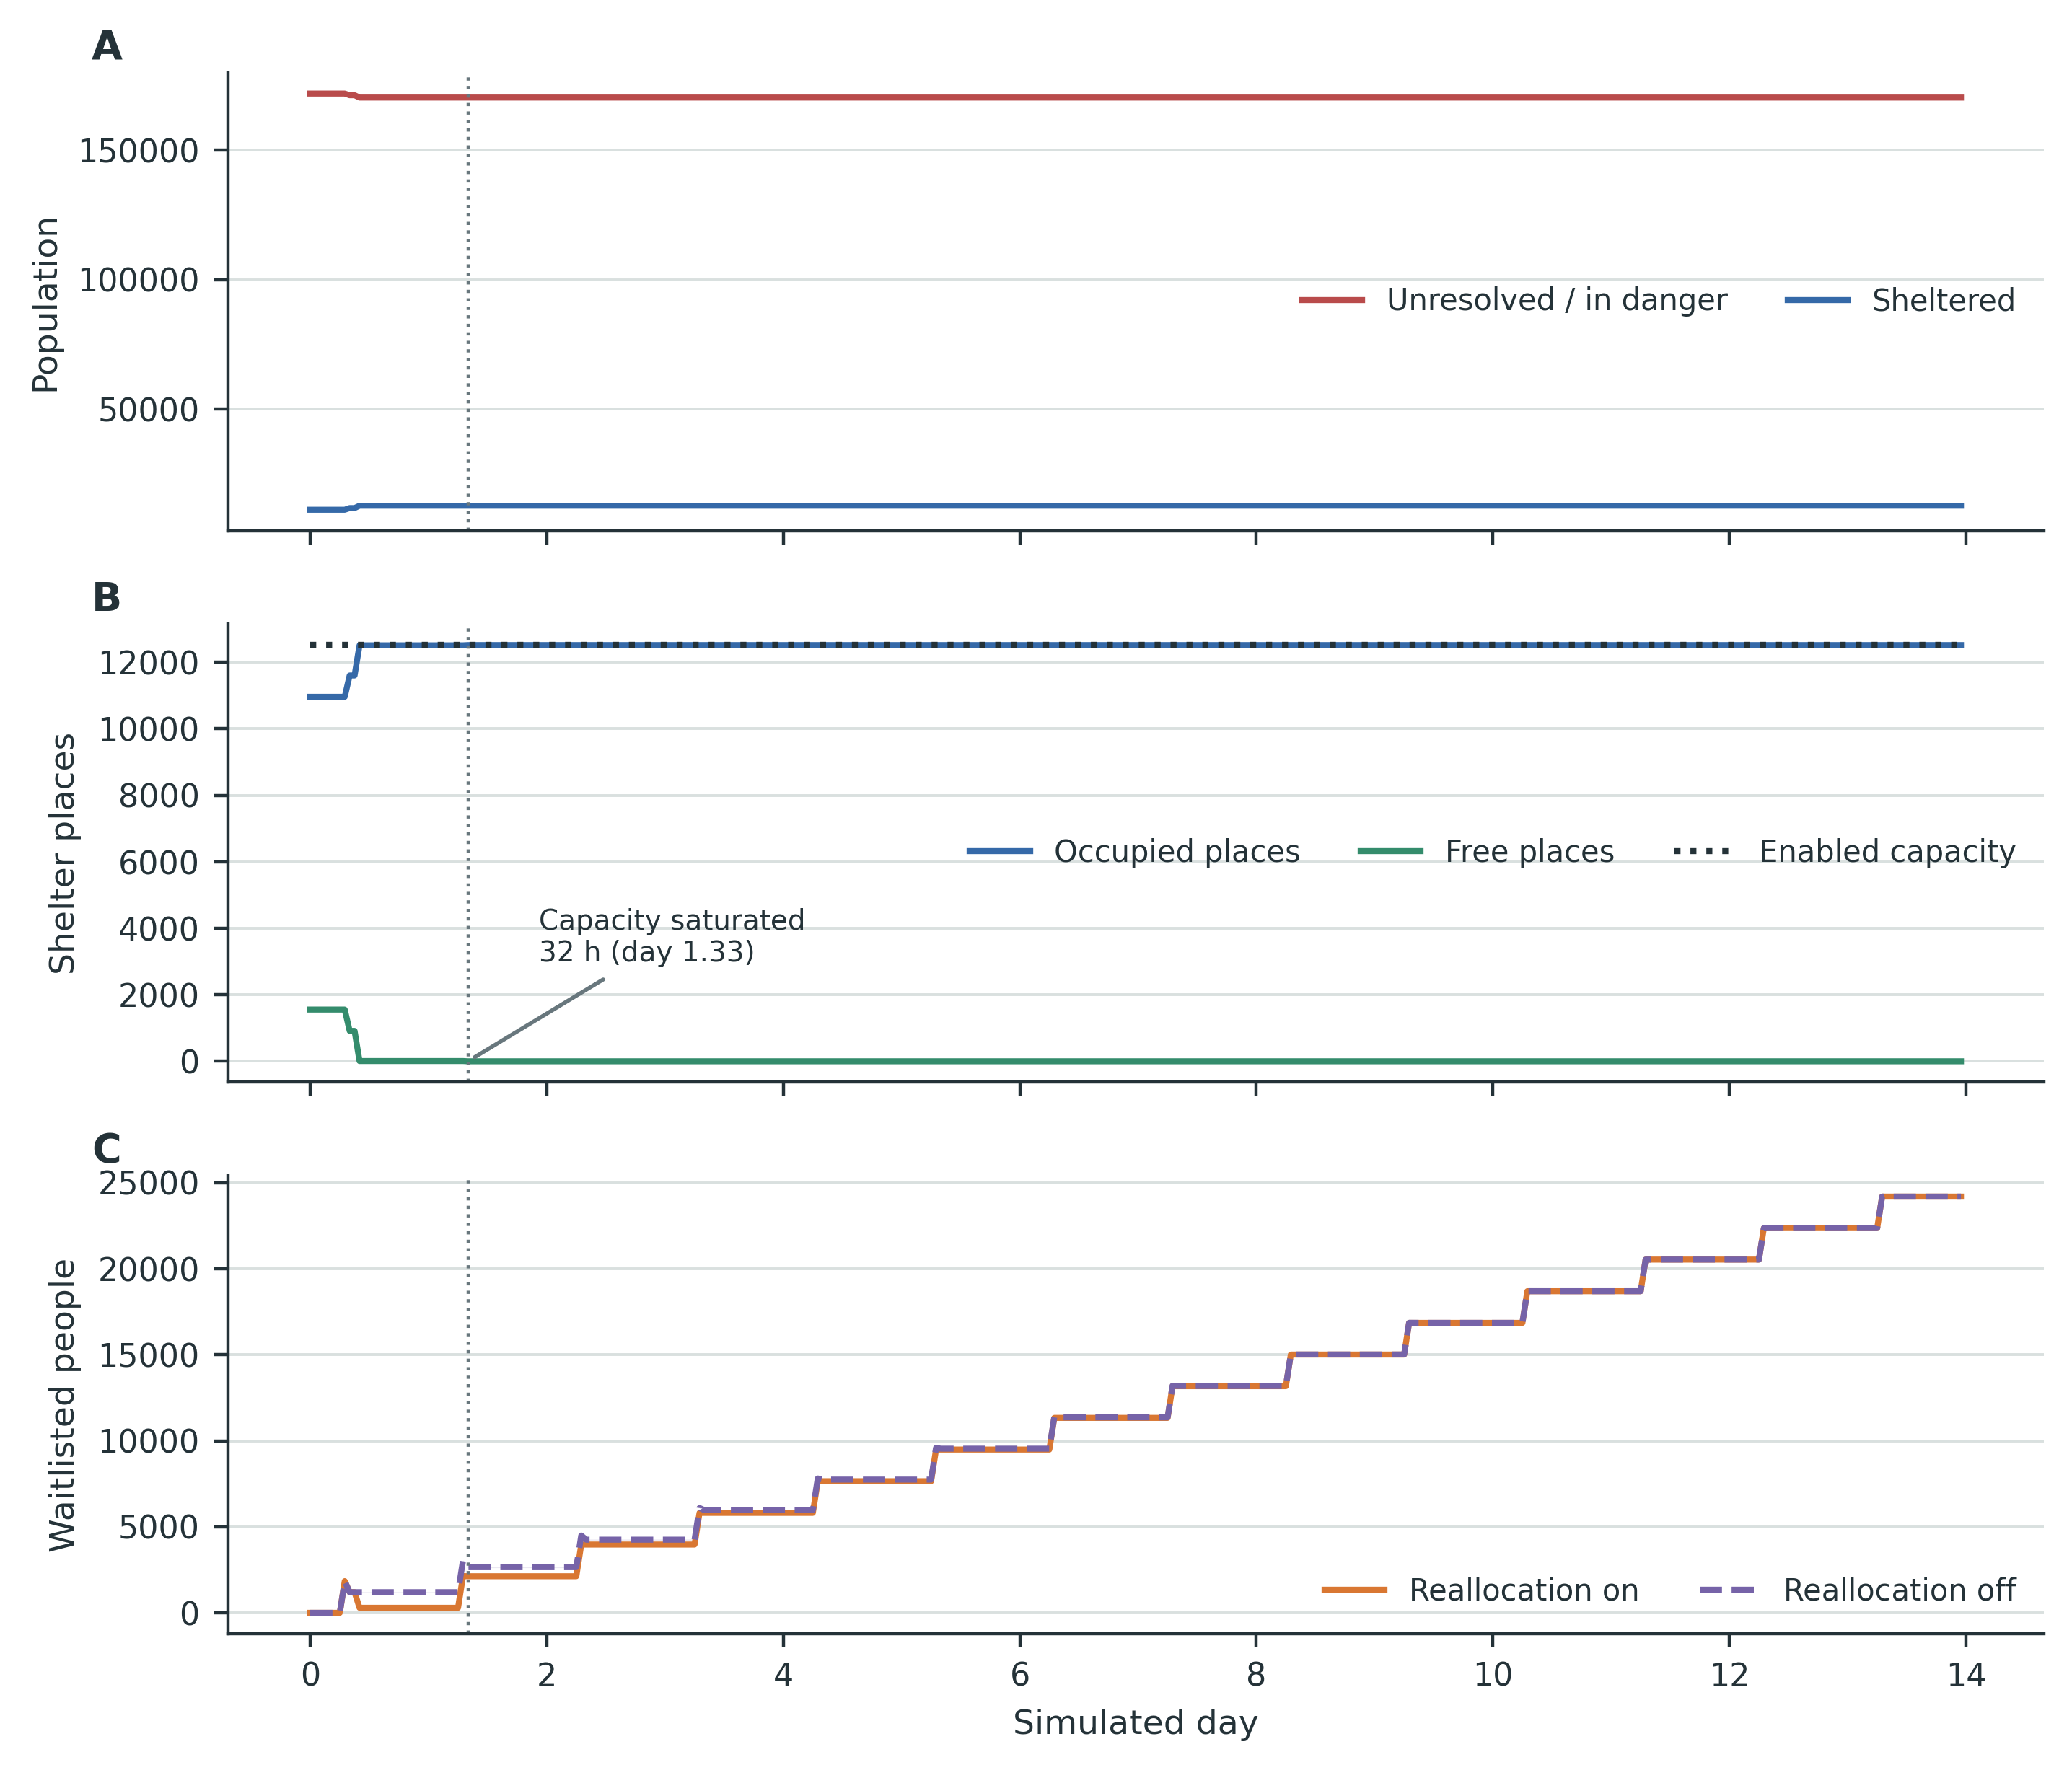
\includegraphics[width=\linewidth]{fig/res-event-disruptions/shelter_reference_dynamics.png}
    \caption{Temporal evolution of the reference shelter experiment over 14 simulated days. Lines show hourly means over five simulation runs. (a) Sheltered and unresolved exposed population with reallocation enabled. (b) Occupied places, free places, and enabled shelter capacity. (c) Total waitlist with reallocation enabled and disabled. The vertical dotted line marks exhaustion of the reference capacity after 32 simulated hours.}
    \label{fig:shelter_reference_dynamics}
\end{figure}

%

The reference scenario therefore illustrates that final coverage alone does not fully characterize evacuation performance. Once capacity is exhausted, redistribution cannot increase the number of people accommodated, but it can reduce how long populations remain waiting for admission.
%SO: tinha gostado mais do meu texto, mas depois vi que tinha uma proxima section sobre isso - VALIDAR
%GA: mantive como esta dada as proximas sections
%These results also highlight a limitation of reallocation when total shelter capacity is fixed. Once the available network reaches full occupancy, redistributing unresolved demand can reduce accumulated waiting but cannot increase final protection. In a real emergency response, however, shelter capacity may evolve over time as new facilities are opened or existing facilities are expanded. Within LODUS, such behavior could be represented by an additional plugin that dynamically creates or activates shelter POIs in response to demand, exposure, or capacity conditions. This would enable future experiments to investigate not only how populations are allocated among existing shelters, but also how adaptive changes to the shelter network could improve protection under evolving demand.

This result suggests that, once the existing shelter network becomes capacity constrained, improving population allocation alone is insufficient and additional shelter capacity is required, motivating the capacity analysis presented next.


\subsubsection{Capacity and Evacuation Demand}
\label{sec:shelter_capacity_response}

The next scenarios examine how shelter capacity and the rate at which exposed populations seek accommodation determine final protection and congestion. Figure~\ref{fig:shelter_sensitivity} summarizes these comparisons.

%SO: nào tem a e b na fig
%GA: são as colunas ao invés de subfigures, ajustei a caption
\begin{figure}[ht]
    \centering
    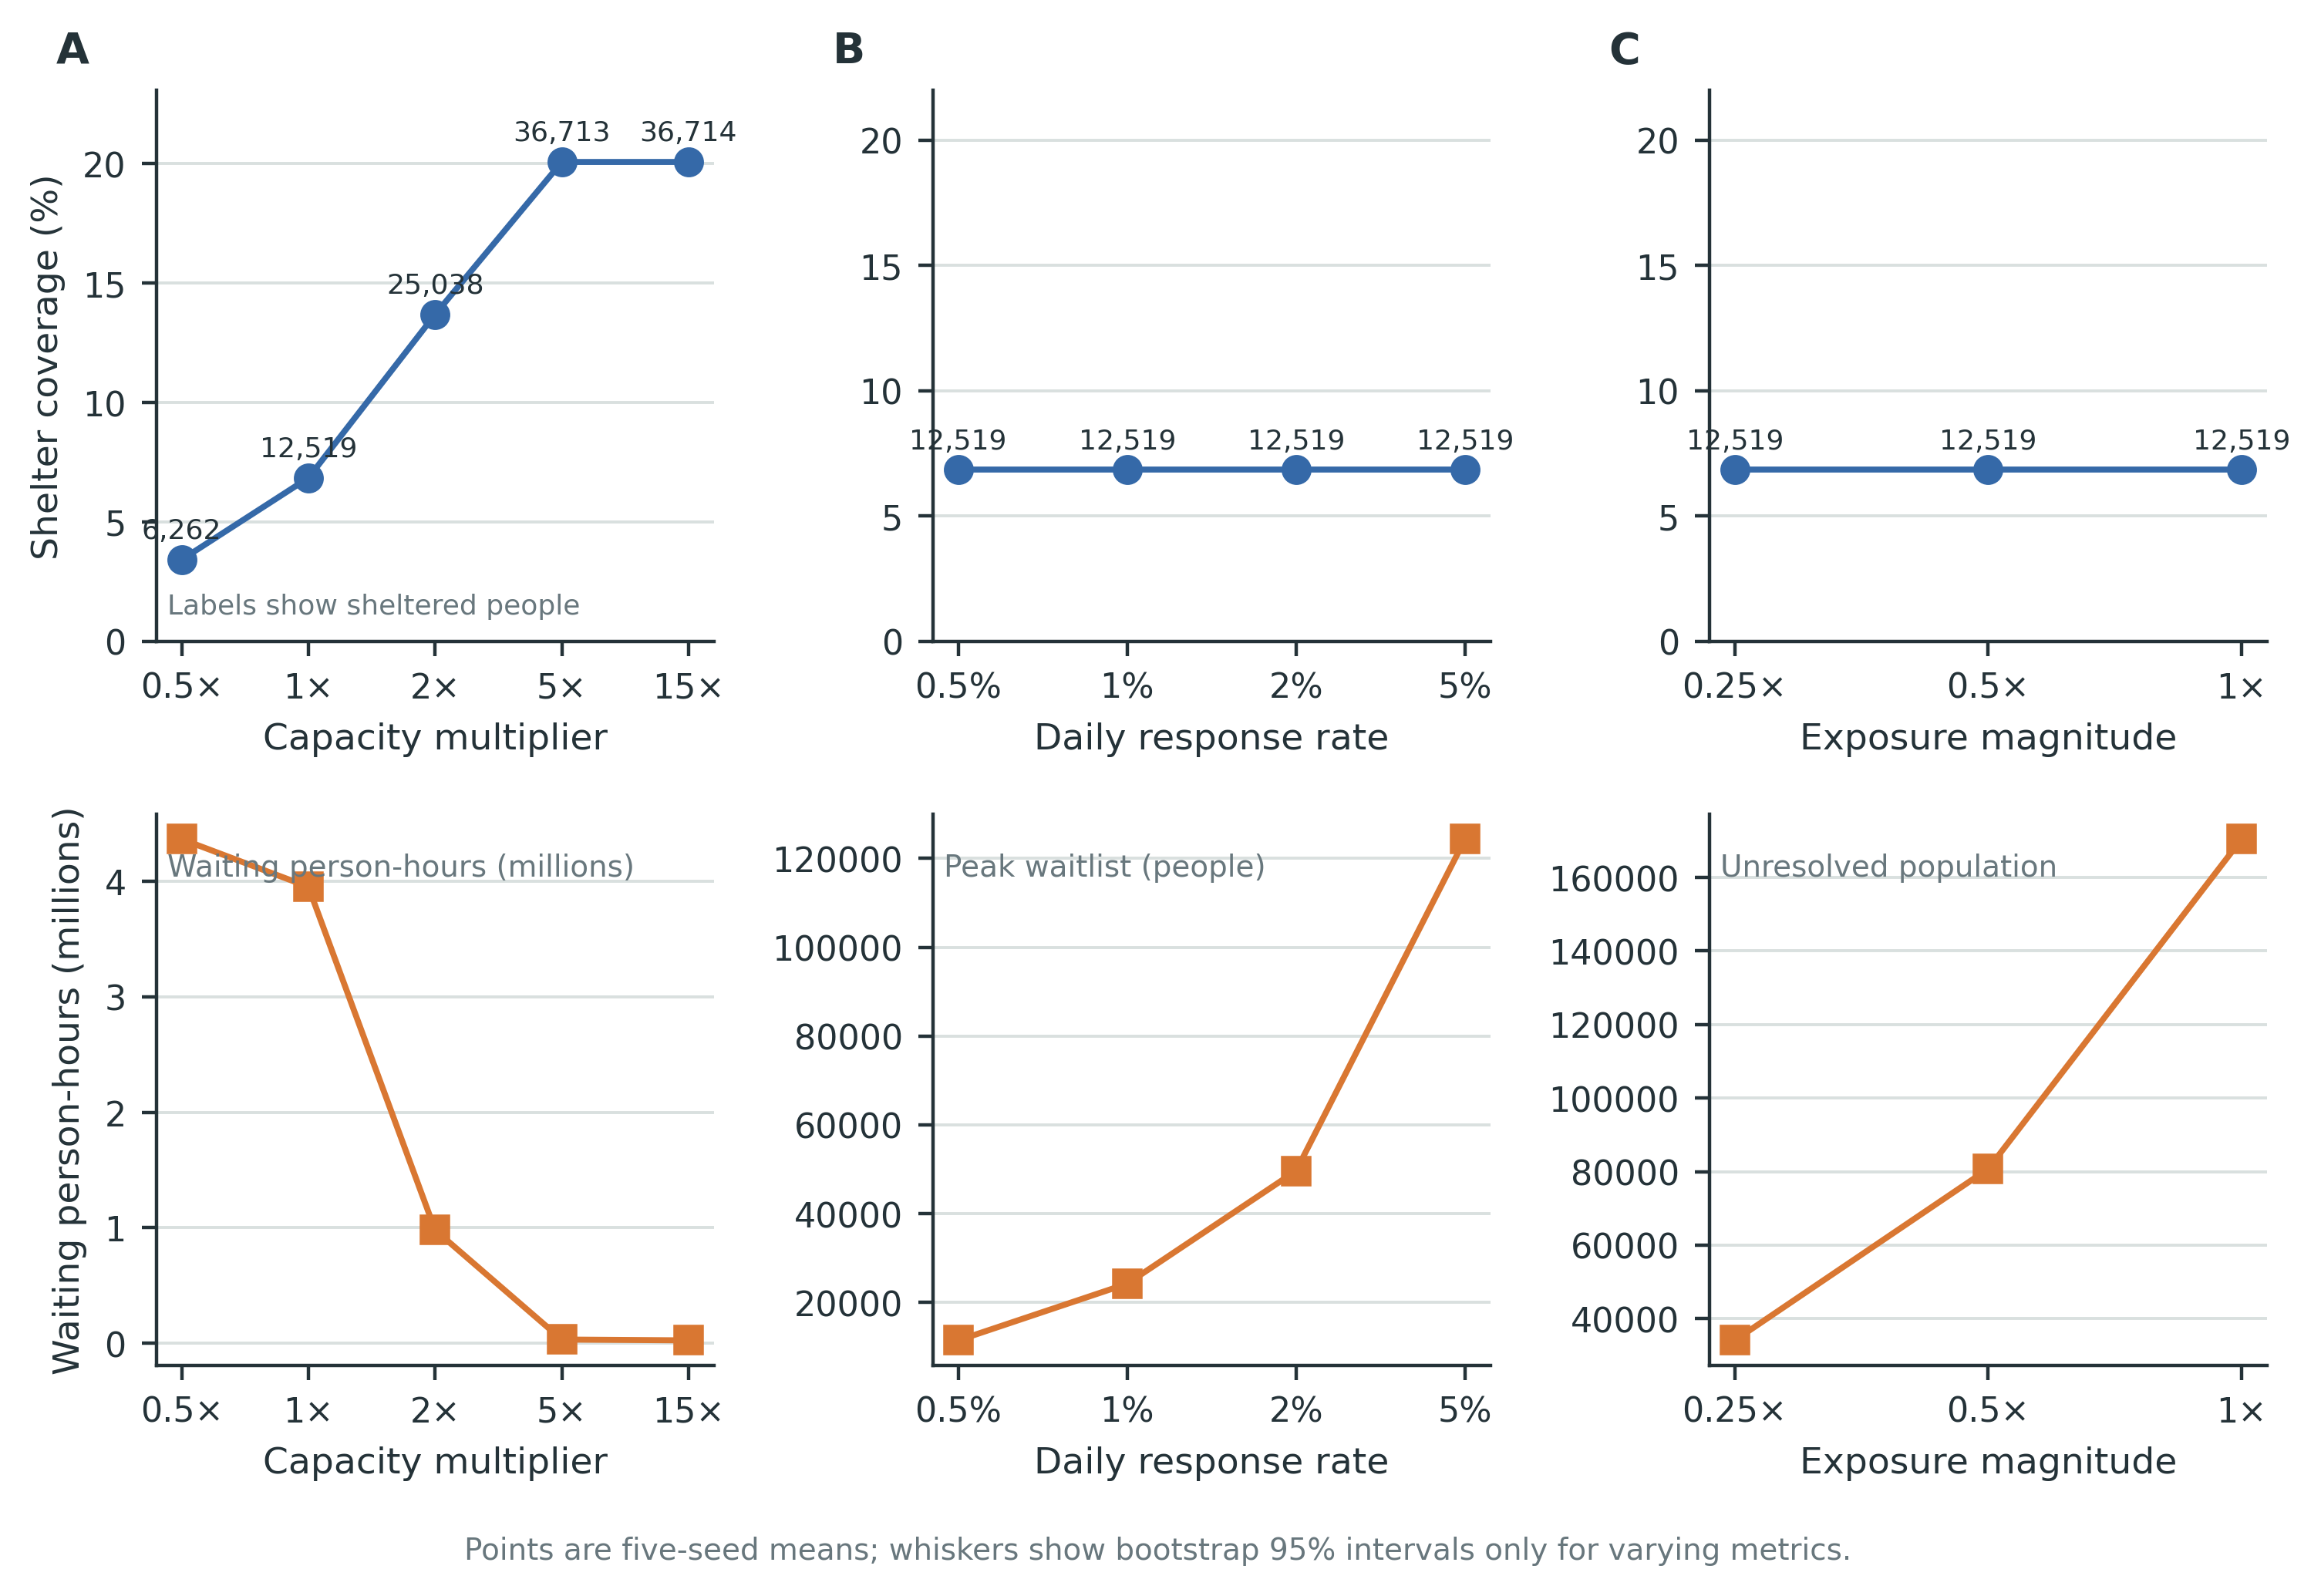
\includegraphics[width=\linewidth]{fig/res-event-disruptions/shelter_sensitivity.png}
    \caption{Shelter outcomes to three scenario parameters: (A) available shelter capacity, (B) daily response rate, and (C) exposure magnitude. The upper row reports final shelter coverage, with labels indicating the number of sheltered people, while the lower row reports the corresponding congestion or unresolved-demand metric: accumulated waiting person-hours for capacity, peak waitlist size for response rate, and unresolved population for exposure magnitude.}
    \label{fig:shelter_sensitivity}
\end{figure}

Increasing shelter capacity substantially improves protection while accommodation remains the principal constraint. Halving the reference capacity reduces final coverage to 3.42\%, whereas doubling it increases coverage to 13.69\%. At five times the reference capacity, coverage reaches approximately 20.07\%.

Increasing capacity further to fifteen times the reference value produces essentially no additional protection during the 14-day simulation. The limiting factor therefore changes as capacity increases. At lower capacity levels, the number of available shelter places limits the population that can be accommodated. Once sufficient capacity exists, the 1\%-per-day response rate and finite simulation duration determine how many exposed people reach shelters before the experiment ends.

Increasing capacity also substantially reduces congestion. Accumulated waiting falls from approximately 3.95 million person-hours under the reference capacity to 0.98 million at twice the capacity and approximately 0.03 million at five times the capacity. The peak waitlist follows the same pattern, falling from 24,195 people to 11,676 and approximately 1,843, respectively.

Changing the daily response rate while keeping capacity fixed produces a different outcome. Final coverage remains 6.843\% for all evaluated response rates because even the slowest condition eventually fills the available shelter network. Higher response rates instead cause this fixed capacity to be consumed earlier and substantially increase queue formation.

At a 0.5\% daily response rate, the peak waitlist is approximately 11,400 people and accumulated waiting is 1.75 million person-hours. At 2\%, these values increase to approximately 49,600 people and 8.36 million person-hours. At 5\%, the peak waitlist exceeds 124,000 people and accumulated waiting reaches approximately 21.4 million person-hours.
Thus, faster evacuation demand does not necessarily result in greater protection. When accommodation remains fixed, it primarily changes how quickly the available places are consumed and how much unresolved demand accumulates around the shelter network.

Exposure scaling provides a complementary demand-side result. Reducing the exposed population does not change the final sheltered population under the reference capacity: all three exposure conditions eventually occupy the same 12,519 places. Lower exposure nevertheless reduces unresolved demand and accumulated waiting. This reinforces the same general relationship between demand and available accommodation without introducing a different limiting mechanism.

Together, these scenarios identify two distinct operating conditions. When shelter space is scarce relative to demand, capacity determines final protection and response speed mainly affects congestion. When capacity becomes sufficiently large, the rate at which exposed populations seek shelter and the duration of the simulation become the principal limits.


\subsubsection{Shelter Failures and Reallocation}
\label{sec:shelter_failures}

The final scenarios examine the effect of losing part of the shelter network. Two disruption conditions are retained. The first disables the single largest shelter, removing 495 places. The second disables the 11 highest-capacity shelters, corresponding to approximately 10\% of the shelter network and removing a combined 3,967 places.

Table~\ref{tbl:shelter_failures} summarizes their effect on final protection with reallocation enabled.

\begin{table}[ht]
\centering
\footnotesize
\caption{Mean shelter outcomes under facility failures over five simulation runs with waitlist reallocation enabled.}
\label{tbl:shelter_failures}
\begin{tabular}{@{}lrrr@{}}
\toprule
\textbf{Condition} &
\shortstack{\textbf{Coverage}\\\textbf{(\%)}} &
\textbf{Unresolved} &
\shortstack{\textbf{Capacity}\\\textbf{removed}} \\
\midrule
No shelter failure
    & 6.843 & 170,417 & --- \\
Largest shelter disabled
    & 6.573 & 170,912 & 495 \\
Top 10\% Highest-capacity shelters disabled
    & 4.675 & 174,384 & 3,967 \\
\bottomrule
\end{tabular}
\end{table}

Disabling the largest shelter reduces coverage from 6.843\% to 6.573\%. Disabling the 11 highest-capacity shelters has a substantially larger effect, reducing coverage to 4.675\%. The difference reflects the amount of accommodation removed from the network: the second condition removes approximately eight times as many places as the failure of the largest individual shelter.

Reallocation cannot restore this lost capacity, but it can reduce congestion among the facilities that remain available. Compared with the corresponding failure scenarios without reallocation, accumulated waiting decreases by approximately 47,000 person-hours after the largest-shelter failure and by 35,000 person-hours after the high-capacity-shelter failures.

\begin{comment}
    
\begin{figure}[ht]
    \centering
    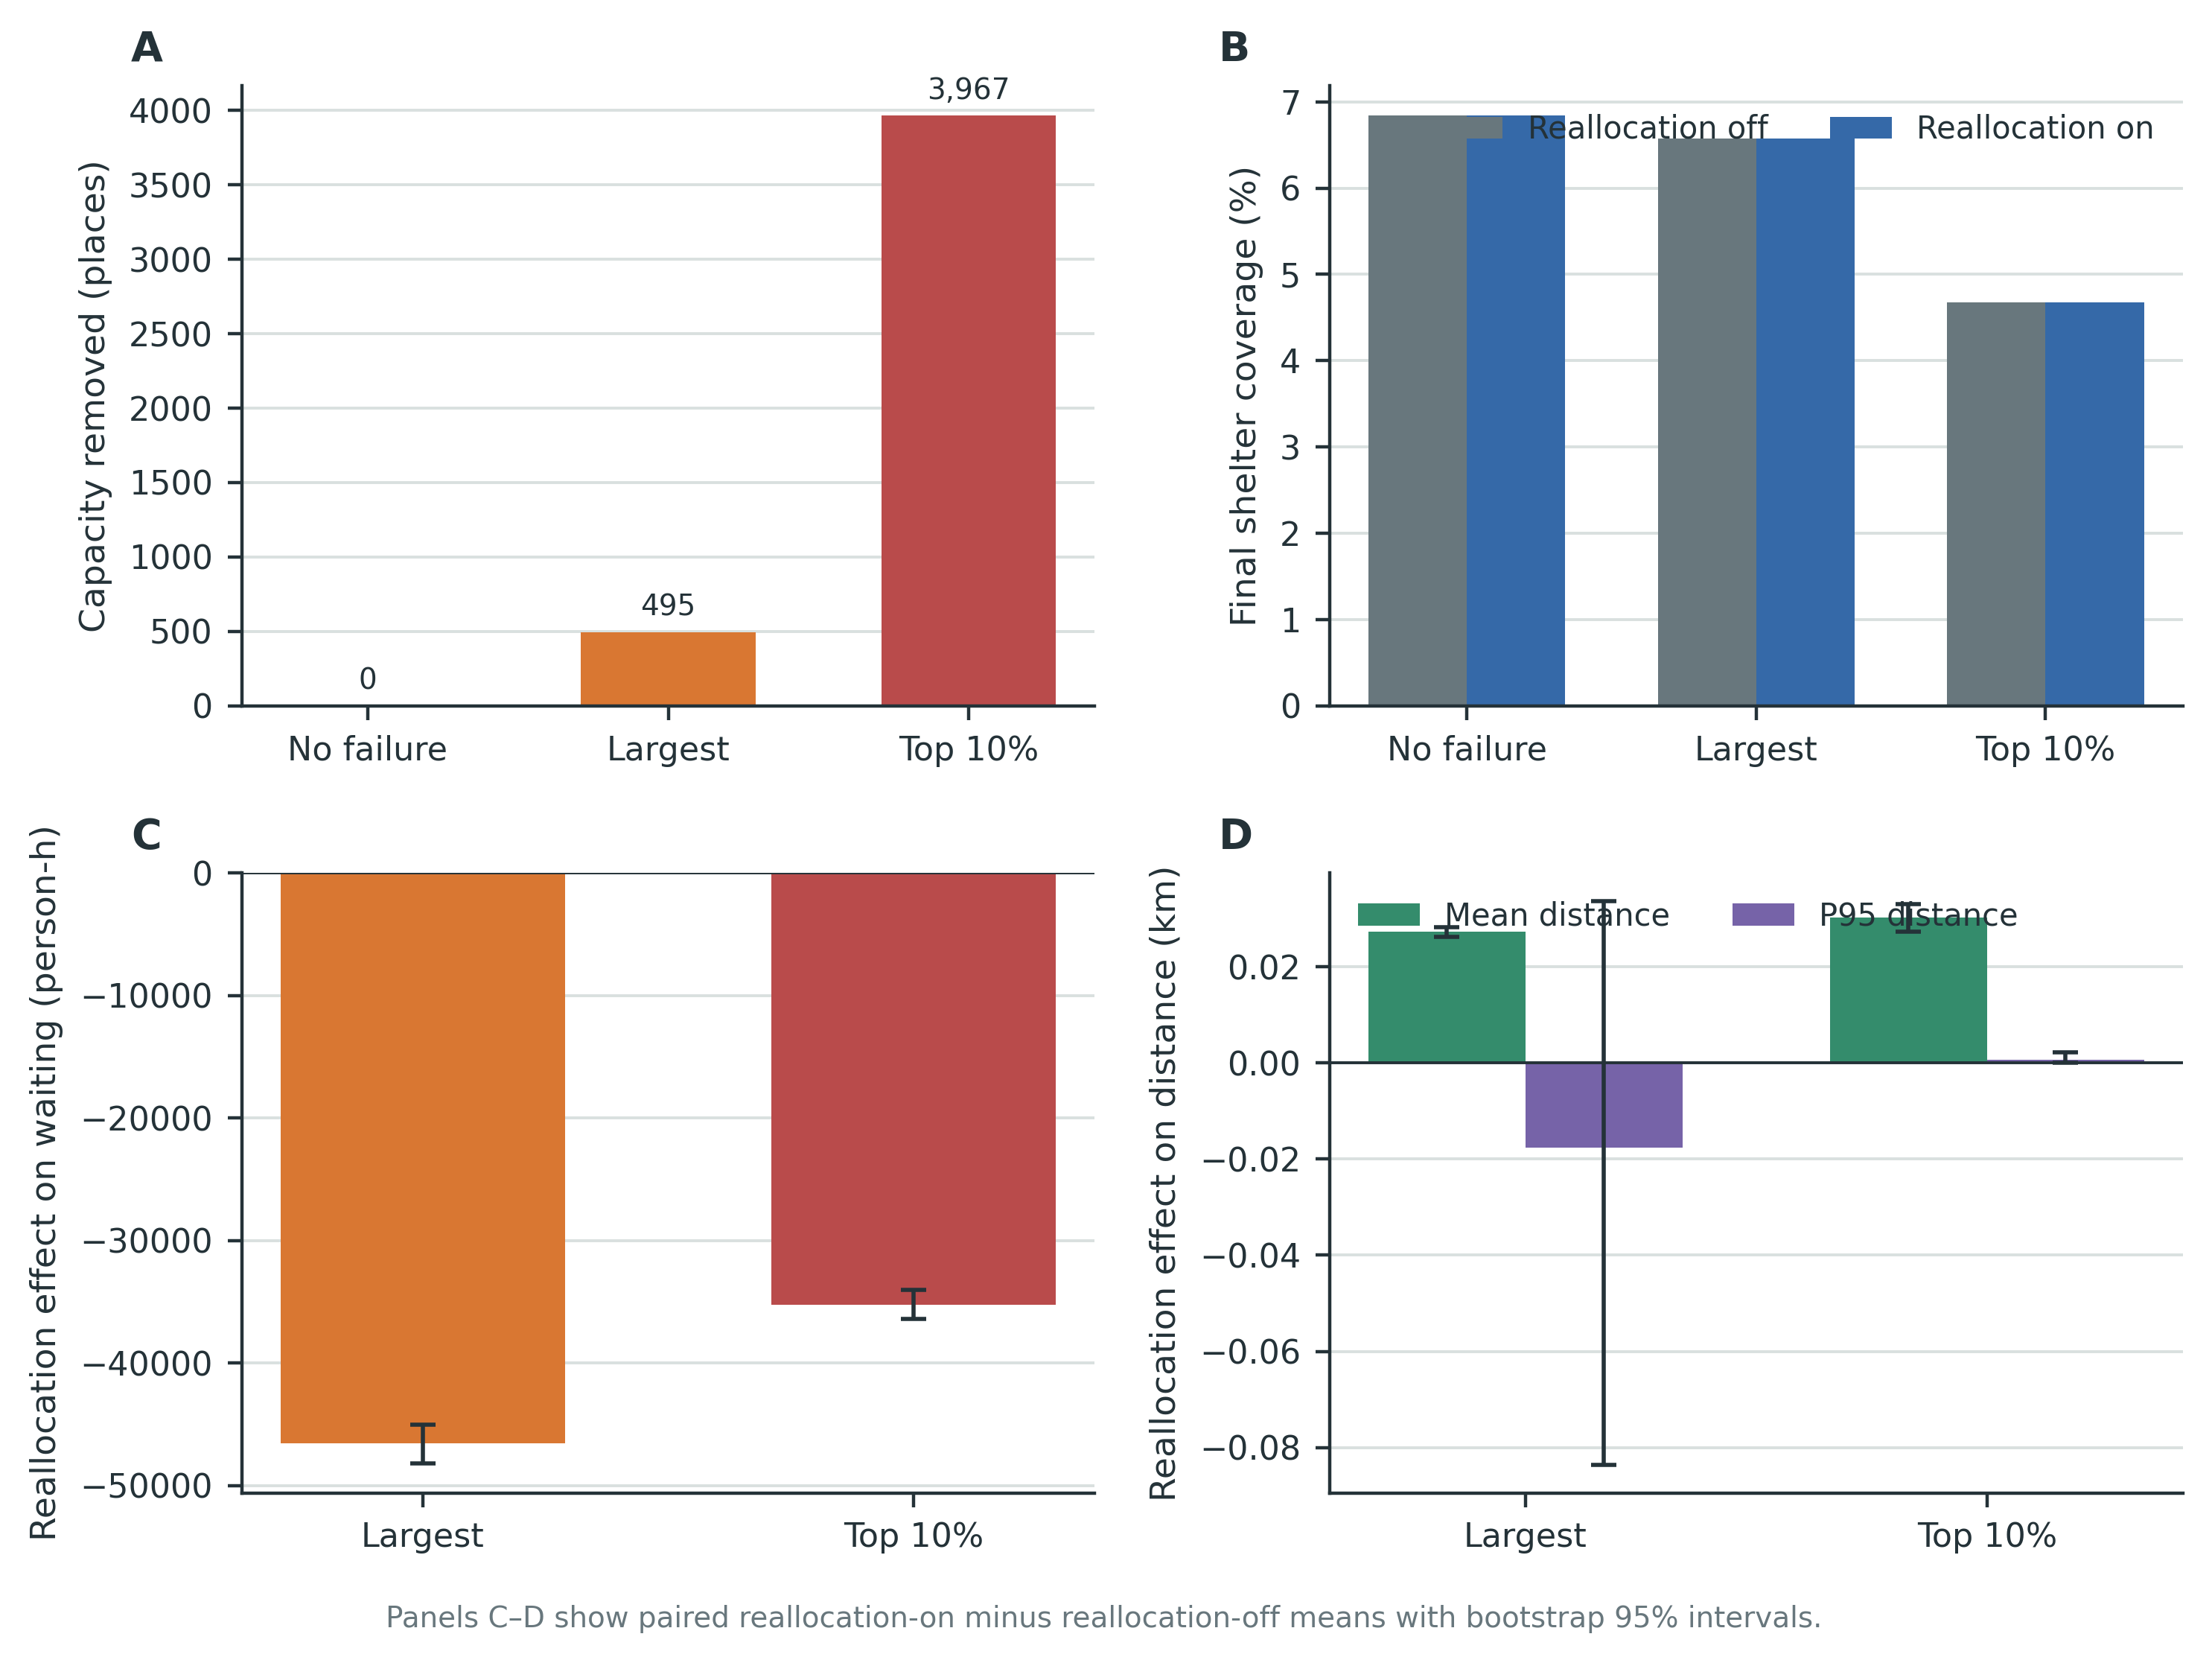
\includegraphics[width=\linewidth]{fig/res-event-disruptions/shelter_failure_robustness.png}
    \caption{Effect of shelter failures and waitlist reallocation on evacuation outcomes. The figure compares the loss of shelter capacity and final coverage under each failure condition and the corresponding reduction in accumulated waiting when reallocation is enabled.}
    \label{fig:shelter_failure_robustness}
\end{figure}
\end{comment}

The failure scenarios reinforce the distinction between accommodation and redistribution. Removing shelter capacity directly reduces the maximum population that can be protected. Reallocation can make better use of the facilities that remain available and reduce waiting, but it cannot recreate the lost accommodation.

Overall, the shelter experiments show that evacuation outcomes depend on the interaction between demand and available service capacity. Under the reference conditions, shelter capacity is exhausted early, limiting final protection while continued evacuation requests generate unresolved demand and congestion. Increasing capacity improves protection until the response rate and simulation horizon become limiting, whereas increasing response speed alone mainly accelerates queue formation. Facility failures further reduce the available protection, while reallocation mitigates waiting without replacing lost capacity. These results demonstrate how exceptional mobility toward a constrained service network differs from the gathering demand examined in the large-scale-event scenarios.





\subsection{Main Findings}
\label{sec:exceptional_disruption_findings}

The experiments in this section examine different ways in which population mobility departs from the normal-life conditions established in the preceding section. Large-scale events introduce additional demand while preserving the availability of the environment, flooding removes some of the origins and destinations required by recurring mobility, and shelter evacuation introduces new movement toward a capacity-constrained service network. Together, these scenarios show that temporary changes in demand and location availability can produce substantially different mobility outcomes even when they operate over the same underlying population and environment representations.

The large-scale-event experiments show that exceptional gathering demand affects both the volume and spatial distribution of movement. Events requesting the same population quantity produce similar aggregate increases when evaluated individually, while their different locations result in distinct displacement-distance distributions. When several events occur simultaneously, their effects are not additive because successive requests operate on a shared and evolving population distribution. Event timing is also relevant: distributing the same four event requests over the day produces more displacement than concentrating them at a single simulation step.

The flood experiments demonstrate how changes in location availability affect different forms of recurring mobility. Activity demand is affected primarily by unavailable destinations, whereas work and school commutes depend on both their origins and their specific destinations. Allowing unavailable activity destinations to be substituted restores almost all requested visits, but shifts part of the disruption into additional travel and increased demand at alternative locations. The same adaptation does not restore work or school attendance because these destinations are not treated as interchangeable in the evaluated configuration. Thus, maintaining mobility demand may require accepting other costs rather than eliminating the effect of the disruption.

The shelter experiments extend this analysis from disrupted recurring mobility to movement generated directly in response to exposure. Under the reference conditions, the shelter network reaches its available capacity early in the simulation, after which additional evacuation demand primarily contributes to unresolved demand and waiting. Increasing shelter capacity improves protection until the response rate and simulation duration become the limiting factors. Conversely, increasing the rate at which exposed populations seek shelter does not increase final protection when capacity remains fixed and instead accelerates congestion. Reallocation reduces waiting by redistributing demand among available facilities, but it cannot increase protection once all available places are occupied or replace capacity removed by shelter failures.

Overall, the results distinguish several consequences of exceptional conditions that would be obscured by considering population movement alone. Additional demand can compete for the population already engaged in other activities; unavailable locations can suppress movement or require alternative destinations; and protective movement can remain constrained by the capacity and availability of the services toward which the population is directed. These experiments therefore complement the normal-life results by showing how the same population representation can support additional demand, mobility disruption, adaptation, and evacuation while preserving the different constraints associated with each scenario.
%GA: não gostei tanto do nome da section
\section{Health-Related Processes and Services}
\label{sec:results_health_processes_services}

The final set of experiments examines processes in which population mobility interacts with health-related state changes and access to recurring services. Unlike the preceding experiments, where the principal outcomes are population movement, activity fulfillment, or displacement, these scenarios introduce outcomes associated with the evolution of population health states and the ability of service facilities to meet recurring demand.

Two applications are considered. The first examines epidemic contagion and evaluates how changes in transmission intensity, vaccination schedules, and movement restrictions alter the progression of infection. The second examines access to dialysis treatment under service-capacity constraints and disruptions to clinics and supporting infrastructure. The corresponding plugins, state representations, service inputs, and infrastructure dependencies are described in Section~\ref{sec:health_processes_services}.%; the present section focuses on the experimental configurations and the resulting population- and service-level outcomes.

Accordingly, these experiments address three broader questions: (i) how population-level health states evolve when contagion operates together with normal-life mobility; (ii) how configured interventions modify this progression; and (iii) how recurring healthcare demand responds to limitations in service capacity and infrastructure availability. Because the epidemic and dialysis experiments use different populations, spatial representations, simulation horizons, and outcome definitions, quantitative comparisons are performed within each experiment group rather than between them.


\subsection{Experimental Overview}
\label{sec:health_results_overview}

The health-related experiments are organized into two main groups. The epidemic experiments use the neighborhood-level representation of Porto Alegre and extend the normal-life mobility baseline with infection and vaccination states. They first vary the configured infection intensity and subsequently evaluate vaccination and movement-restriction scenarios. These experiments correspond to the configurations originally reported with the publisehd manuscript~\cite{silva2026lodusPop}.

The dialysis experiments instead use the reduced and complete census-sector environments. They examine recurring treatment demand under differences in demand, clinic availability, water-infrastructure dependencies, environmental disruption, recovery, and the spatial distribution of unavailable treatment capacity.

Table~\ref{tbl:health_results_overview} summarizes the principal experiment groups. All simulations use 24 steps per cycle, with each step representing one hour. A cycle therefore represents one simulated day in both experiment groups, although their simulation horizons differ substantially.

\begin{table}[ht]
\centering
\footnotesize
\setlength{\tabcolsep}{4pt}
\caption{Health-related experiment groups and their principal comparisons.}
\label{tbl:health_results_overview}
\begin{tabularx}{\linewidth}{@{}p{3.0cm}p{3.0cm}p{1.6cm}X@{}}
\toprule
\textbf{Experiment} &
\textbf{Environment} &
\textbf{Duration} &
\textbf{Principal comparison} \\
\midrule

Infection intensity
& Neighborhood-level environment
& 500 days
& $R_0$ values of 2.6, 3.07, and 6.0 are compared to examine the effect of transmission intensity on epidemic progression. \\

Vaccination
& Neighborhood-level environment
& 500 days
& An unvaccinated reference is compared with four vaccination schedules that vary the number, timing, and modeled effectiveness of vaccine doses. \\

Vaccination and movement restriction
& Neighborhood-level environment
& 500 days
& Restriction values of 0, 0.50, and 0.75 are combined with either no vaccination or Vaccination C. \\

Dialysis access and resilience
& Reduced and complete census-sector environments
& 10 days
& Recurring treatment is evaluated under reference conditions, excess demand, facility outages, flooding, infrastructure dependencies, recovery, and alternative spatial patterns of clinic failure. \\

Dialysis demand sensitivity
& Reduced and complete census-sector environments
& 10 days
& Demand-to-capacity ratios from approximately 0.25 to 1.25 are evaluated to identify when waiting and incomplete treatment emerge under the configured service network. \\

\bottomrule
\end{tabularx}
\end{table}


\subsection{Epidemic Contagion and Mitigation}
\label{sec:results_epidemic_contagion}

The epidemic experiments combine the neighborhood-level normal-life mobility configuration with the infection and vaccination mechanisms described in Sections~\ref{sec:infection_plugin_inputs} and~\ref{sec:vaccination_plugin_inputs}. The full neighborhood representation contains 94 regions, 504 base POIs, and a population of 1,409,351. The mobility configuration follows the neighborhood-level reference introduced in Section~\ref{sec:routine_mobility_neighborhood}, using a L\'evy scale of 2.

Each epidemic simulation covers 500 simulated days. At initialization, 50 individuals in each neighborhood are assigned the infected state, resulting in 4,700 initially infected individuals across the city; the remaining population begins susceptible and no population begins in the removed state. The removal parameter is held at $\gamma=1/15$ throughout the experiments. Infection is evaluated as the population moves among POIs, so the population present at each location determines the susceptible and infected groups involved in each local contagion update.

Three comparisons are performed. First, the infection-intensity experiment varies $R_0$ while preserving the remaining epidemic and mobility configuration. Second, the $R_0=2.6$ configuration is used to compare four vaccination schedules. Finally, the same reference configuration is used to examine vaccination together with progressively stronger reductions in routine mobility.


\subsubsection{Transmission Intensity and Epidemic Dynamics}
\label{sec:results_epidemic_transmission}

The first experiment examines how the configured infection intensity changes epidemic progression. Three values of the basic reproduction number are considered: $R_0=2.6$, $R_0=3.07$, and $R_0=6.0$. These values were selected based on estimates reported for COVID-19 transmission in Brazil~\cite{dutra2020covidR0,deSouza2020covirR0,dutra2021covidR0}. With $\gamma=1/15$ held constant, the corresponding infection-rate parameters are $\beta=0.1733$, $0.204$, and $0.4$, respectively.

Figure~\ref{fig:epidemic_transmission_dynamics}a presents cumulative infections over the 500 simulated days. Cumulative infections include the 4,700 individuals infected at initialization together with subsequent transitions from susceptible to infected. Increasing $R_0$ produces faster epidemic progression and a larger cumulative infected population over the simulated period. The three configurations differ only in the infection parameterization within this comparison, while the mobility behavior and initial epidemic state remain unchanged.

The $R_0=2.6$ configuration is retained as the reference for the remaining epidemic experiments. This run reaches a cumulative total of 875,962 infected individuals. Figure~\ref{fig:epidemic_transmission_dynamics}b provides a complementary view by showing the susceptible, currently infected, and removed populations over time. Unlike cumulative infections, the infected-state population represents only individuals that are infected at a particular point in the simulation. In the reference run, this population reaches its maximum on day 247, when 81,528 individuals are simultaneously in the infected state.

\begin{figure}[!ht]
\centering

\begin{subfigure}{0.96\textwidth}
    \centering
    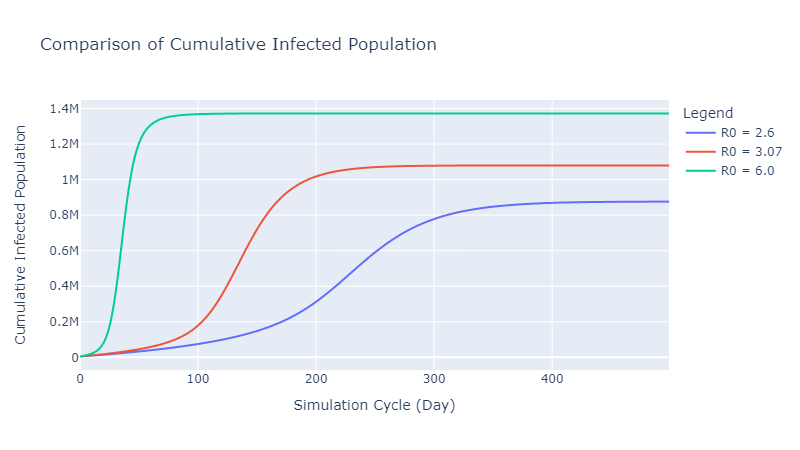
\includegraphics[width=\linewidth]{fig/res-health/InfectedR0.png}
    \caption{Cumulative infected population for $R_0=2.6$, $3.07$, and $6.0$.}
    \label{fig:epidemic_r0}
\end{subfigure}

\vspace{0.5em}

\begin{subfigure}{0.96\textwidth}
    \centering
    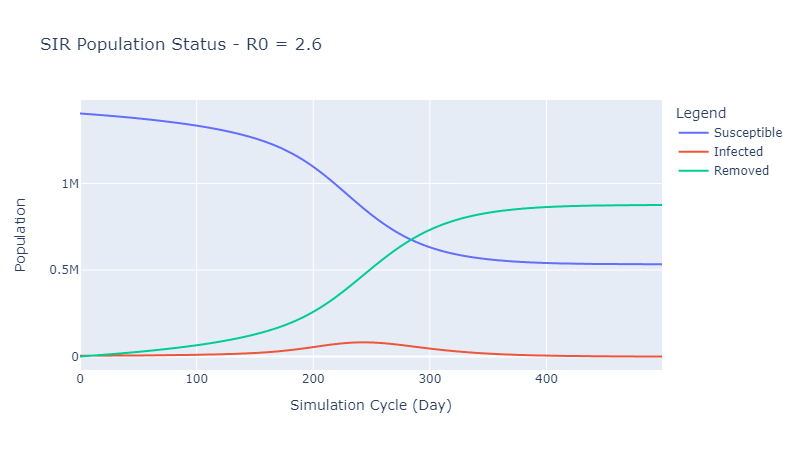
\includegraphics[width=\linewidth]{fig/res-health/SIRPopulationStatus.png}
    \caption{Susceptible, infected, and removed populations over time for the $R_0=2.6$ reference configuration.}
    \label{fig:epidemic_sir_status}
\end{subfigure}

\caption{Epidemic progression under the neighborhood-level configuration. Panel (a) compares cumulative infections under different basic reproduction numbers, while panel (b) shows the population occupying each SIR state for the $R_0=2.6$ reference. Cumulative infections and the population currently infected represent distinct measures of epidemic progression.}
\label{fig:epidemic_transmission_dynamics}
\end{figure}

These results establish two complementary effects of the infection configuration. The cumulative trajectories show the sensitivity of epidemic progression to the configured transmission intensity, while the SIR trajectory illustrates how cumulative incidence differs from the number of individuals simultaneously infected. The $R_0=2.6$ configuration provides the common reference used in the following intervention experiments.


\subsubsection{Vaccination Schedules}
\label{sec:results_epidemic_vaccination}

The second experiment examines vaccination while holding the epidemic configuration at $R_0=2.6$. Daily vaccination quantities follow the Porto Alegre vaccination series described in Section~\ref{sec:vaccination_plugin_inputs} and are distributed among the modeled regions in proportion to their populations. Four vaccination configurations are considered. Configurations A--C introduce progressively larger numbers of doses and associated effectiveness values, while Vaccination D represents an intentionally idealized single-dose configuration with complete modeled effectiveness.

Table~\ref{tbl:epidemic_vaccination_results} summarizes the dose schedules together with the cumulative infection total recorded for each published run. The unvaccinated $R_0=2.6$ simulation is included as the common reference.

\begin{table}[ht]
\centering
\setlength{\tabcolsep}{5pt}
\caption{Published vaccination configurations and cumulative infection outcomes for $R_0=2.6$. Effectiveness values correspond to the modeled reduction in susceptible-to-infected transitions associated with each vaccination level.}
\label{tbl:epidemic_vaccination_results}
\begin{tabularx}{\linewidth}{@{}lcp{3.2cm}p{2.4cm}X@{}}
\toprule
\textbf{Configuration} &
\textbf{Doses} &
\textbf{Effectiveness by dose} &
\textbf{Starting days} &
\textbf{Cumulative infections} \\
\midrule

No vaccination
& 0
& --
& --
& 875,962 \\

Vaccination A
& 1
& 0.4
& 50
& 440,569 \\

Vaccination B
& 2
& 0.4, 0.7
& 50, 150
& 360,607 \\

Vaccination C
& 3
& 0.4, 0.7, 1.0
& 50, 150, 250
& 355,124 \\

Vaccination D
& 1
& 1.0
& 50
& 170,978 \\

\bottomrule
\end{tabularx}
\end{table}

Figure~\ref{fig:epidemic_vaccination} shows how these differences accumulate over time. Even the single-dose Vaccination A configuration substantially reduces cumulative infections relative to the unvaccinated reference, from 875,962 to 440,569. Introducing the second dose in Vaccination B further reduces the total to 360,607. Vaccination C reaches a similar final value of 355,124, while the idealized Vaccination D configuration produces the lowest cumulative total, with 170,978 infections.

The temporal trajectories are particularly informative for Vaccination B and Vaccination C. Both configurations use the same effectiveness values and starting days for their first two doses and therefore remain similar during the initial portion of the simulation. Their configurations diverge when the third dose of Vaccination C begins on day 250. The resulting difference in final cumulative infections is comparatively small relative to the reduction already produced by the first two vaccination levels. This comparison should therefore be interpreted as a difference between complete vaccination schedules rather than as an isolated estimate of the effect of an additional dose.

\begin{figure}[!ht]
\centering
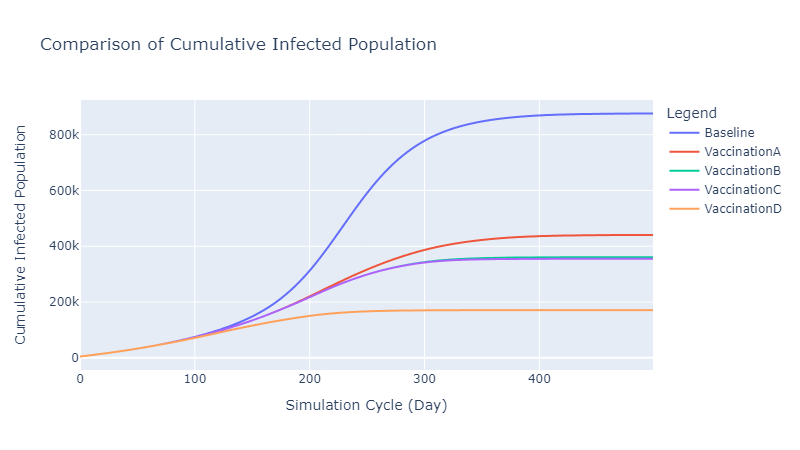
\includegraphics[width=0.96\linewidth]{fig/res-health/InfectedVaccines.png}
\caption{Cumulative infected population under the unvaccinated $R_0=2.6$ reference and Vaccination A--D configurations. The schedules vary in the number of doses, their modeled effectiveness, and their starting days, as summarized in Table~\ref{tbl:epidemic_vaccination_results}.}
\label{fig:epidemic_vaccination}
\end{figure}

Vaccination D provides a useful upper-bound comparison within the implemented behavior, but its effectiveness of 1.0 after a single dose is intentionally idealized. Vaccination C is therefore used instead in the following combined-intervention experiment, since its progressive three-dose schedule provides a less idealized configuration for examining vaccination together with changes in mobility.


\subsubsection{Vaccination and Movement Restriction}
\label{sec:results_epidemic_vaccination_restriction}

The final epidemic experiment examines the combined effect of vaccination and reduced normal-life movement. The epidemic configuration remains fixed at $R_0=2.6$, while movement restriction is varied among 0, 0.50, and 0.75. As described in Section~\ref{sec:levy_walk_plugin_inputs}, the restriction parameter reduces the population selected for the affected routine movements rather than modifying the epidemiological parameters directly. Each restriction value is evaluated both without vaccination and with Vaccination C, producing six configurations.

Figure~\ref{fig:epidemic_vaccination_restriction} presents the cumulative infection trajectories. Relative to the unrestricted and unvaccinated reference, increasing movement restriction reduces the progression of cumulative infections. Vaccination C produces a larger reduction than movement restriction alone, while combining vaccination with stronger movement reduction produces the lowest infection totals.

The strongest combined configuration uses Vaccination C together with a movement restriction of 0.75. This run reaches 140,941 cumulative infections, compared with 875,962 in the unrestricted and unvaccinated reference. This corresponds to an 83.91\% reduction in cumulative infections under the evaluated configuration.

\begin{figure}[ht]
\centering
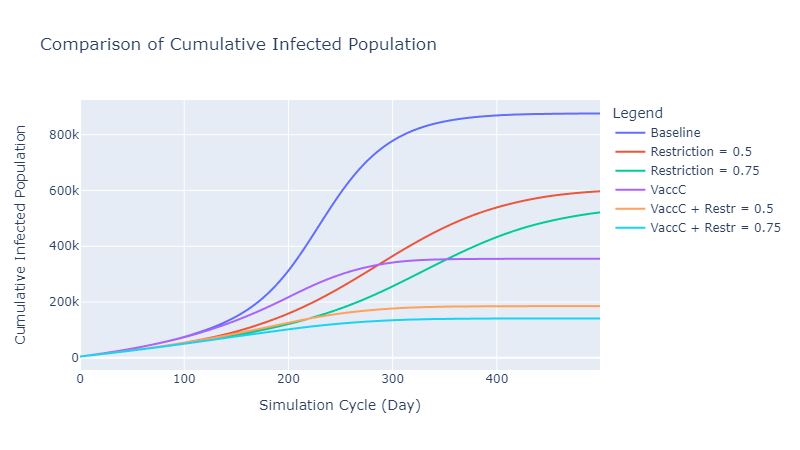
\includegraphics[width=0.96\linewidth]{fig/res-health/InfectedVaccineRestriction.png}
\caption{Cumulative infected population for combinations of movement restriction and Vaccination C under $R_0=2.6$. Restriction values of 0, 0.50, and 0.75 are evaluated both without vaccination and with the three-dose Vaccination C configuration.}
\label{fig:epidemic_vaccination_restriction}
\end{figure}

Taken together, the epidemic experiments show how the same population and mobility configuration can be combined with evolving health states and progressively different intervention conditions. Increasing the configured transmission intensity accelerates epidemic progression, while vaccination and reduced movement both lower cumulative infections under the evaluated scenarios. Their combination produces the lowest reported outcome among the non-idealized intervention configurations.

These results should be interpreted as controlled comparisons among configured epidemic scenarios rather than forecasts of COVID-19 transmission in Porto Alegre. The infection mechanism assumes homogeneous SIR parameters within each configuration and local mixing among populations sharing a POI, while vaccine effectiveness and movement reduction are scenario-defined inputs.

\subsection{Dialysis Access and Infrastructure Resilience}
\label{sec:results_dialysis}

The second health-related application examines access to dialysis as a recurring, capacity-constrained service. In contrast to the epidemic experiments, where the principal outcome is a change in population health state, these simulations evaluate whether scheduled treatment demand can be served by a spatially distributed network of clinics whose availability may depend on supporting infrastructure.

The dialysis behavior, infrastructure dependencies, and disruption inputs are described in Section~\ref{sec:dialysis_plugin_inputs} and Section~\ref{sec:dependency_mapping_plugin_inputs}.
Here, the analysis focuses on treatment completion, waiting, unresolved demand, and travel distance under different service and disruption conditions.

All core scenarios cover ten simulated days, with 24 hourly steps per day. Selected patients require treatment every three days, with initial due days distributed across the treatment interval. When treatment becomes due, patients are assigned to the nearest eligible clinic with available capacity; demand that cannot be admitted remains pending and is reconsidered during subsequent hours.

Clinic operating schedules and treatment capacities are modeled as scenario-defined parameters. By default, clinics operate from 06:00 to 18:00 and admit at most two patients per hour. The exceptions are Centro de Diálise e Transplante and Hospital Moinhos de Vento, which operate until 22:00 and admit at most eight and six patients per hour, respectively.

Two census-sector environments are considered. The reduced environment contains 13 regions, 435 residential POIs, 8 dialysis clinics, and 2 water treatment facilities, while the complete environment contains 94 regions, 2,711 residential POIs, 12 clinics, and 6 water treatment facilities. The reference demand level is configured at 50\% of the nominal three-day treatment capacity of each environment, corresponding to 552 patients in the reduced environment and 696 in the complete environment. Controlled disruptions begin at simulation step 78, corresponding to 06:00 on the third simulated day.
Each reported scenario was executed 30 times. Table~\ref{tbl:dialysis_scenarios} summarizes the configurations used in the comparisons. 

\begin{table}[ht]
\centering
\footnotesize
\setlength{\tabcolsep}{4pt}
\caption{Dialysis scenarios and principal configured conditions.}
\label{tbl:dialysis_scenarios}
\begin{tabularx}{\linewidth}{@{}llrX@{}}
\toprule
\textbf{ID} &
\textbf{Environment} &
\textbf{Patients} &
\textbf{Configured condition} \\
\midrule

D01 & Reduced & 552
& Reference demand level, corresponding to 50\% of nominal three-day capacity. \\

D02 & Reduced  & 552
& ETA Moinhos de Vento is disabled at step 78 and remains unavailable. \\

D03 & Reduced  & 552
& The same ETA is disabled at step 78 and restored four hours later. \\

D04 & Reduced  & 552
& Historical water levels directly affect exposed clinics and water treatment facilities. \\

D05 & Reduced  & 552
& A synthetic 10.1~m water level affects water treatment facilities; clinic unavailability propagates through POI dependencies. \\

D06 & Reduced  & 552
& The scheduled ETA Moinhos outage is combined with a synthetic 9.3~m water-level disruption. \\

D07 & Reduced  & 1,380
& Treatment demand is increased to 125\% of nominal three-day capacity without facility disruption. \\

D08 & Reduced  & 552
& One high-capacity clinic is disabled, removing 128 daily treatment slots. \\

D09 & Reduced  & 552
& Four lower-capacity clinics are disabled, also removing 128 daily treatment slots. \\

D10 & Complete & 696
& Complete-environment reference at 50\% of nominal three-day capacity. \\

D11 & Complete & 696
& Synthetic 9.3~m exposure affects clinics and water sources and is combined with the scheduled ETA Moinhos outage. \\

\bottomrule
\end{tabularx}
\end{table}

Table~\ref{tbl:dialysis_results} provides an overview of the mean outcomes across the 30 repeated executions. Coverage represents the proportion of treatment sessions that become due during the simulation and are completed within the ten-day horizon. Waiting is reported as accumulated due-wait patient-hours, thereby accounting for both the number of patients awaiting treatment and the duration of their wait. Overdue sessions are those that remain due at the end of the simulation. Disabled clinic-hours account only for periods of facility unavailability caused by direct or dependency-related disruptions, rather than ordinary closing hours or exhausted treatment capacity. Distance reports the mean geographic distance from the patient origin to the clinic for admitted treatment sessions.

\begin{table}[ht]
\centering
\footnotesize
\setlength{\tabcolsep}{3pt}
\caption{Mean dialysis outcomes across 30 executions.}
\label{tbl:dialysis_results}
\begin{tabularx}{\linewidth}{
    @{}
    l
    >{\raggedright\arraybackslash}X
    rrrrr
    @{}
}
\toprule
\textbf{ID} &
\textbf{Condition} &
\shortstack{\textbf{Coverage}\\\textbf{(\%)}} &
\shortstack{\textbf{Wait}\\\textbf{(patient-h)}} &
\shortstack{\textbf{Overdue}\\\textbf{(sessions)}} &
\shortstack{\textbf{Disabled}\\\textbf{(clinic-h)}} &
\shortstack{\textbf{Distance}\\\textbf{(km)}} \\
\midrule

D01 & Reduced reference demand
    & 100.00 & 16,640 &   0.0 &     0 & 1.836 \\

D02 & Persistent ETA outage
    &  68.52 & 67,608 & 363.5 &   972 & 2.090 \\

D03 & Four-hour ETA outage
    & 100.00 & 17,238 &   0.0 &    24 & 1.838 \\

D04 & Historical direct flood exposure
    & 100.00 & 17,144 &   0.0 &   225 & 1.768 \\

D05 & Synthetic ETA exposure
    &  50.00 & 84,480 & 552.0 & 1,296 & 1.845 \\

D06 & Combined water and ETA disruption
    &  50.00 & 84,480 & 552.0 & 1,296 & 1.845 \\

D07 & Demand above nominal capacity
    &  93.02 & 106,416 & 114.2 &     0 & 1.854 \\

D08 & One high-capacity clinic unavailable
    & 100.00 & 18,670 &   0.0 &   162 & 1.768 \\

D09 & Four lower-capacity clinics unavailable
    & 100.00 & 18,670 &   0.0 &   648 & 2.037 \\

D10 & Complete reference demand
    & 100.00 & 20,700 &   0.0 &     0 & 6.537 \\

D11 & Complete combined disruption
    &  71.43 & 81,126 & 415.3 & 1,458 & 7.052 \\

\bottomrule
\end{tabularx}
\end{table}

\subsubsection{Service Capacity and Demand Pressure}
\label{sec:results_dialysis_capacity}

The reference scenarios first establish whether the configured clinic networks can serve moderate recurring demand in the absence of disruptions. D01 completes all due treatment sessions in the reduced environment, while D10 likewise reaches 100\% coverage in the complete environment. Nevertheless, the simulations accumulate 16,640 and 20,700 due-wait patient-hours, respectively. Complete treatment coverage therefore does not imply that all patients are treated immediately; waiting provides a complementary measure of service pressure even when all demand can eventually be accommodated.

Scenario D07 isolates the consequence of increased demand without disabling any facility. The number of dialysis patients is increased from 552 to 1,380 in the reduced environment, corresponding to 125\% of the nominal treatment capacity available over a three-day treatment interval. Coverage decreases to 93.02\%, accumulated waiting increases to 106,416 patient-hours, and an average of 114.2 sessions remains overdue at the end of the simulation. In contrast to the infrastructure-disruption scenarios, D07 produces these incomplete treatments with zero disabled clinic-hours. The result therefore distinguishes insufficient available service capacity from failures caused by facility unavailability.
The comparison between D01 and D07 shows the two extremes represented in the simulated scenarios: moderate demand that can be fully absorbed; and demand exceeding the nominal capacity of the reduced network. 

An additional analysis fills the interval between them with demand-to-capacity ratios of 0.25, 0.50, 0.90, 1.00, and 1.25. These correspond to 276, 552, 993, 1,104, and 1,380 patients in the reduced environment and 348, 696, 1,254, 1,392, and 1,740 patients in the complete environment.
Figure~\ref{fig:dialysis_demand_sensitivity} shows that both environments retain 100\% coverage through a demand-to-capacity ratio of 1.00, although accumulated waiting rises continuously. In the reduced environment, mean waiting increases from 6,720 patient-hours at a ratio of 0.25 to 46,800 at 1.00; the corresponding values for the complete environment are 8,400 and 57,840 patient-hours. The sharpest change occurs between ratios 1.00 and 1.25. At 1.25, coverage falls to 93.02\% in both environments, while waiting reaches 106,416 patient-hours in the reduced environment and 133,008 in the complete environment.

\begin{figure}[ht]
    \centering
    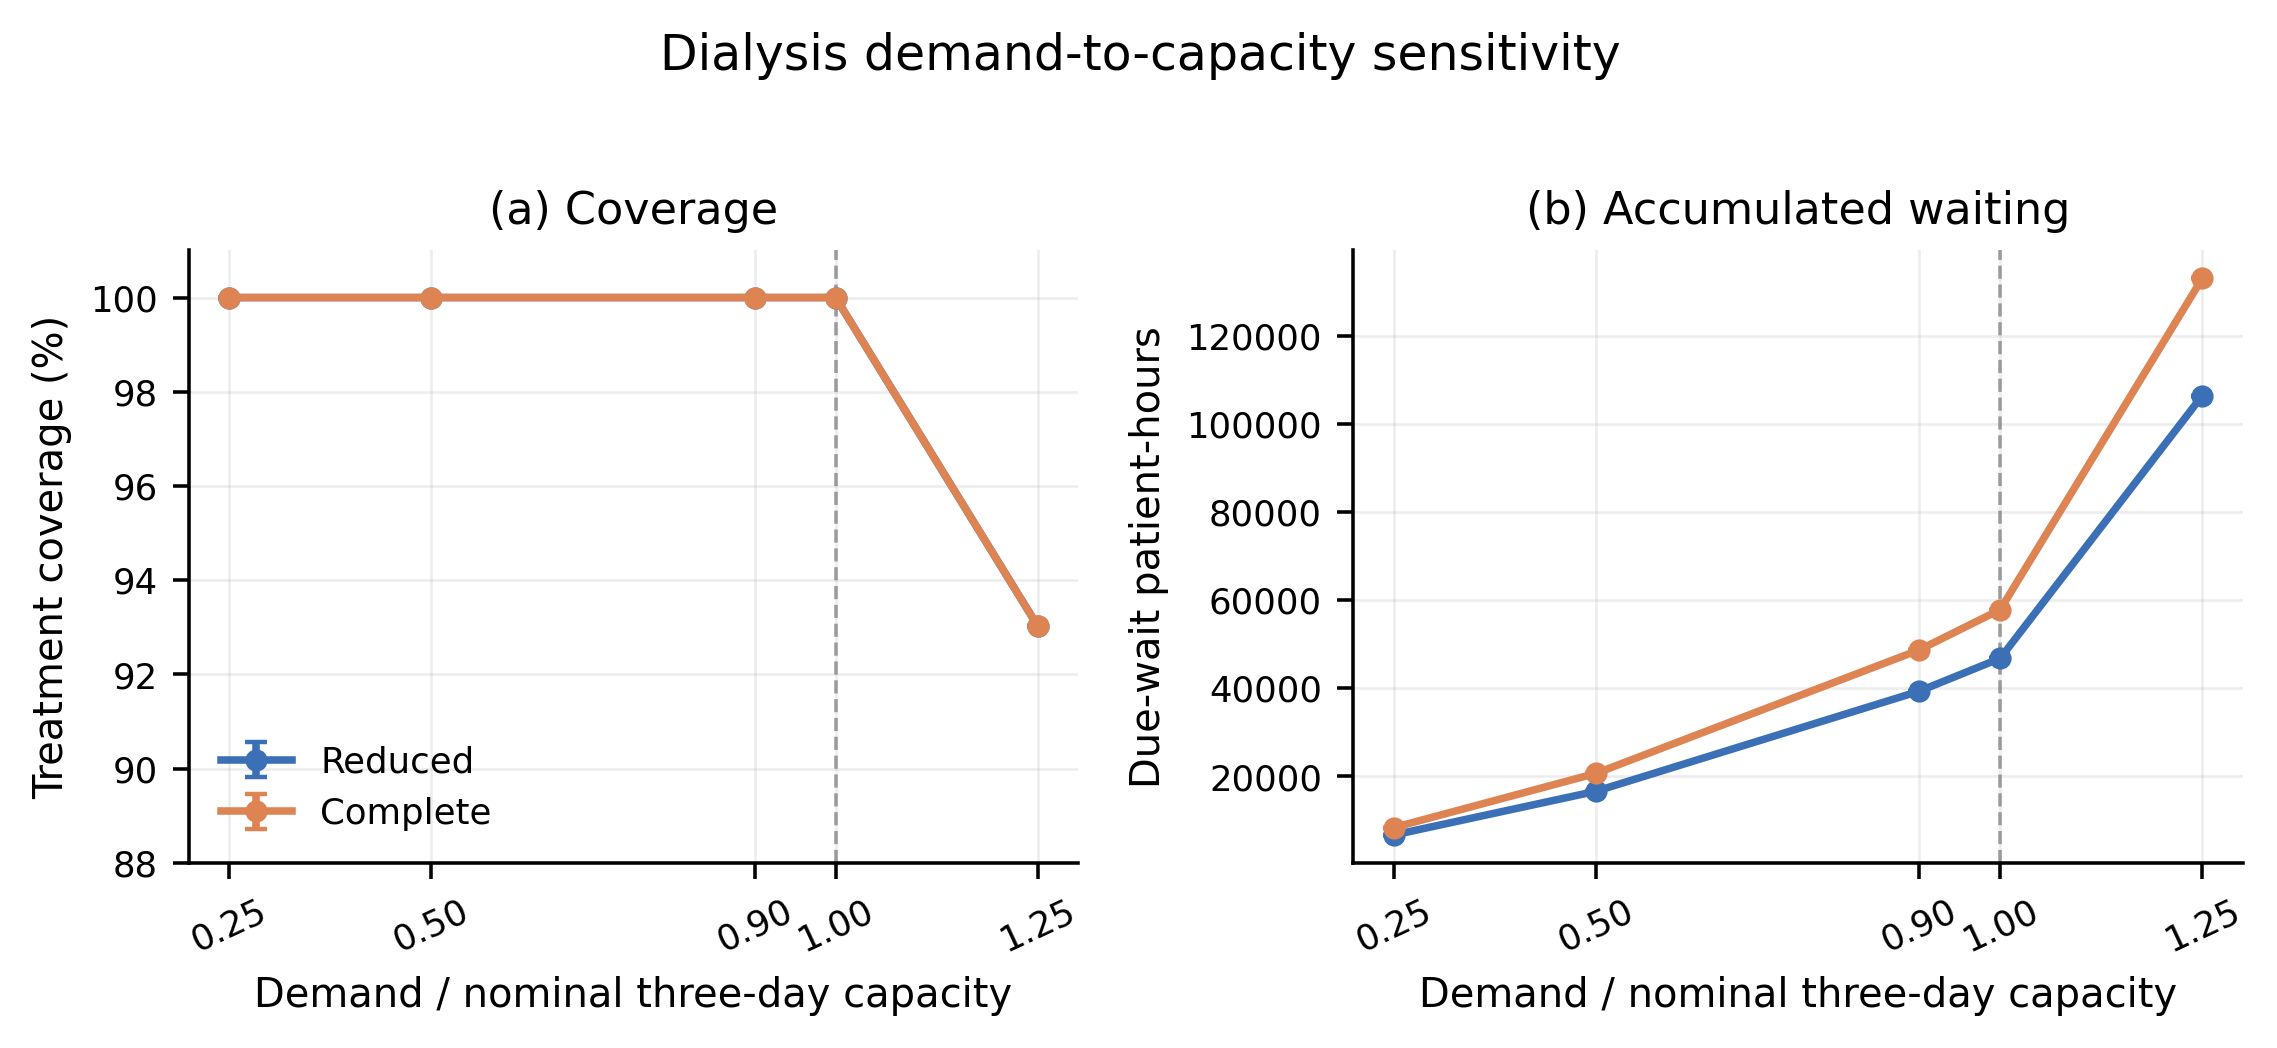
\includegraphics[width=\linewidth]
      {fig/res-health/dialysis_demand_sensitivity.png}
    \caption{Treatment coverage and accumulated waiting under increasing dialysis demand in the reduced and complete census-sector environments. Points show means over 30 simulation executions.}
    \label{fig:dialysis_demand_sensitivity}
\end{figure}


\subsubsection{Infrastructure Disruption and Recovery}
\label{sec:results_dialysis_disruption}

The next scenarios evaluate how service outcomes change when clinic availability is reduced directly or through supporting water infrastructure. D02 and D03 provide the clearest comparison because they begin from the same reduced-environment configuration and apply the same ETA Moinhos de Vento outage at 06:00 on day 3, differing only in whether the facility remains unavailable.

Under the persistent outage in D02, treatment coverage decreases from 100\% in D01 to 68.52\%. Accumulated waiting increases from 16,640 to 67,608 patient-hours, and an average of 363.5 treatment sessions remains overdue at the end of the simulation. The disruption accounts for 972 disabled clinic-hours because clinics dependent on the unavailable ETA remain inaccessible throughout the remaining simulation period.

By contrast, restoring ETA Moinhos de Vento four hours after the initial disruption in D03 is sufficient for all due treatments to be completed within the simulation horizon. Waiting increases only moderately relative to D01, from 16,640 to 17,238 patient-hours, and no sessions remain overdue at the end of the simulation. The comparison therefore shows that the duration of an infrastructure interruption can be more consequential than its occurrence alone: a short interruption creates temporary service pressure, whereas the persistent loss generates a backlog that cannot be cleared within the evaluated period.

The aggregate values, however, do not show how this backlog develops or how quickly service recovers after restoration. Figure~\ref{fig:dialysis_outage_recovery} aligns the hourly response across the 30 simulation runs. The outage begins at step 78 and the D03 restoration occurs at step 82, four hours later. During this interval, available treatment capacity in D03 falls from 26 to 4 slots per hour. After restoration, the number of patients with treatment due and still waiting returns to the D01 level at step 88, six hours after restoration, and cumulative treatment completions catch up with D01 at step 89. In D02, by contrast, only four slots per hour remain available during clinic opening periods after the disruption, so the backlog persists to the end of the simulation.

\begin{figure}[ht]
    \centering
    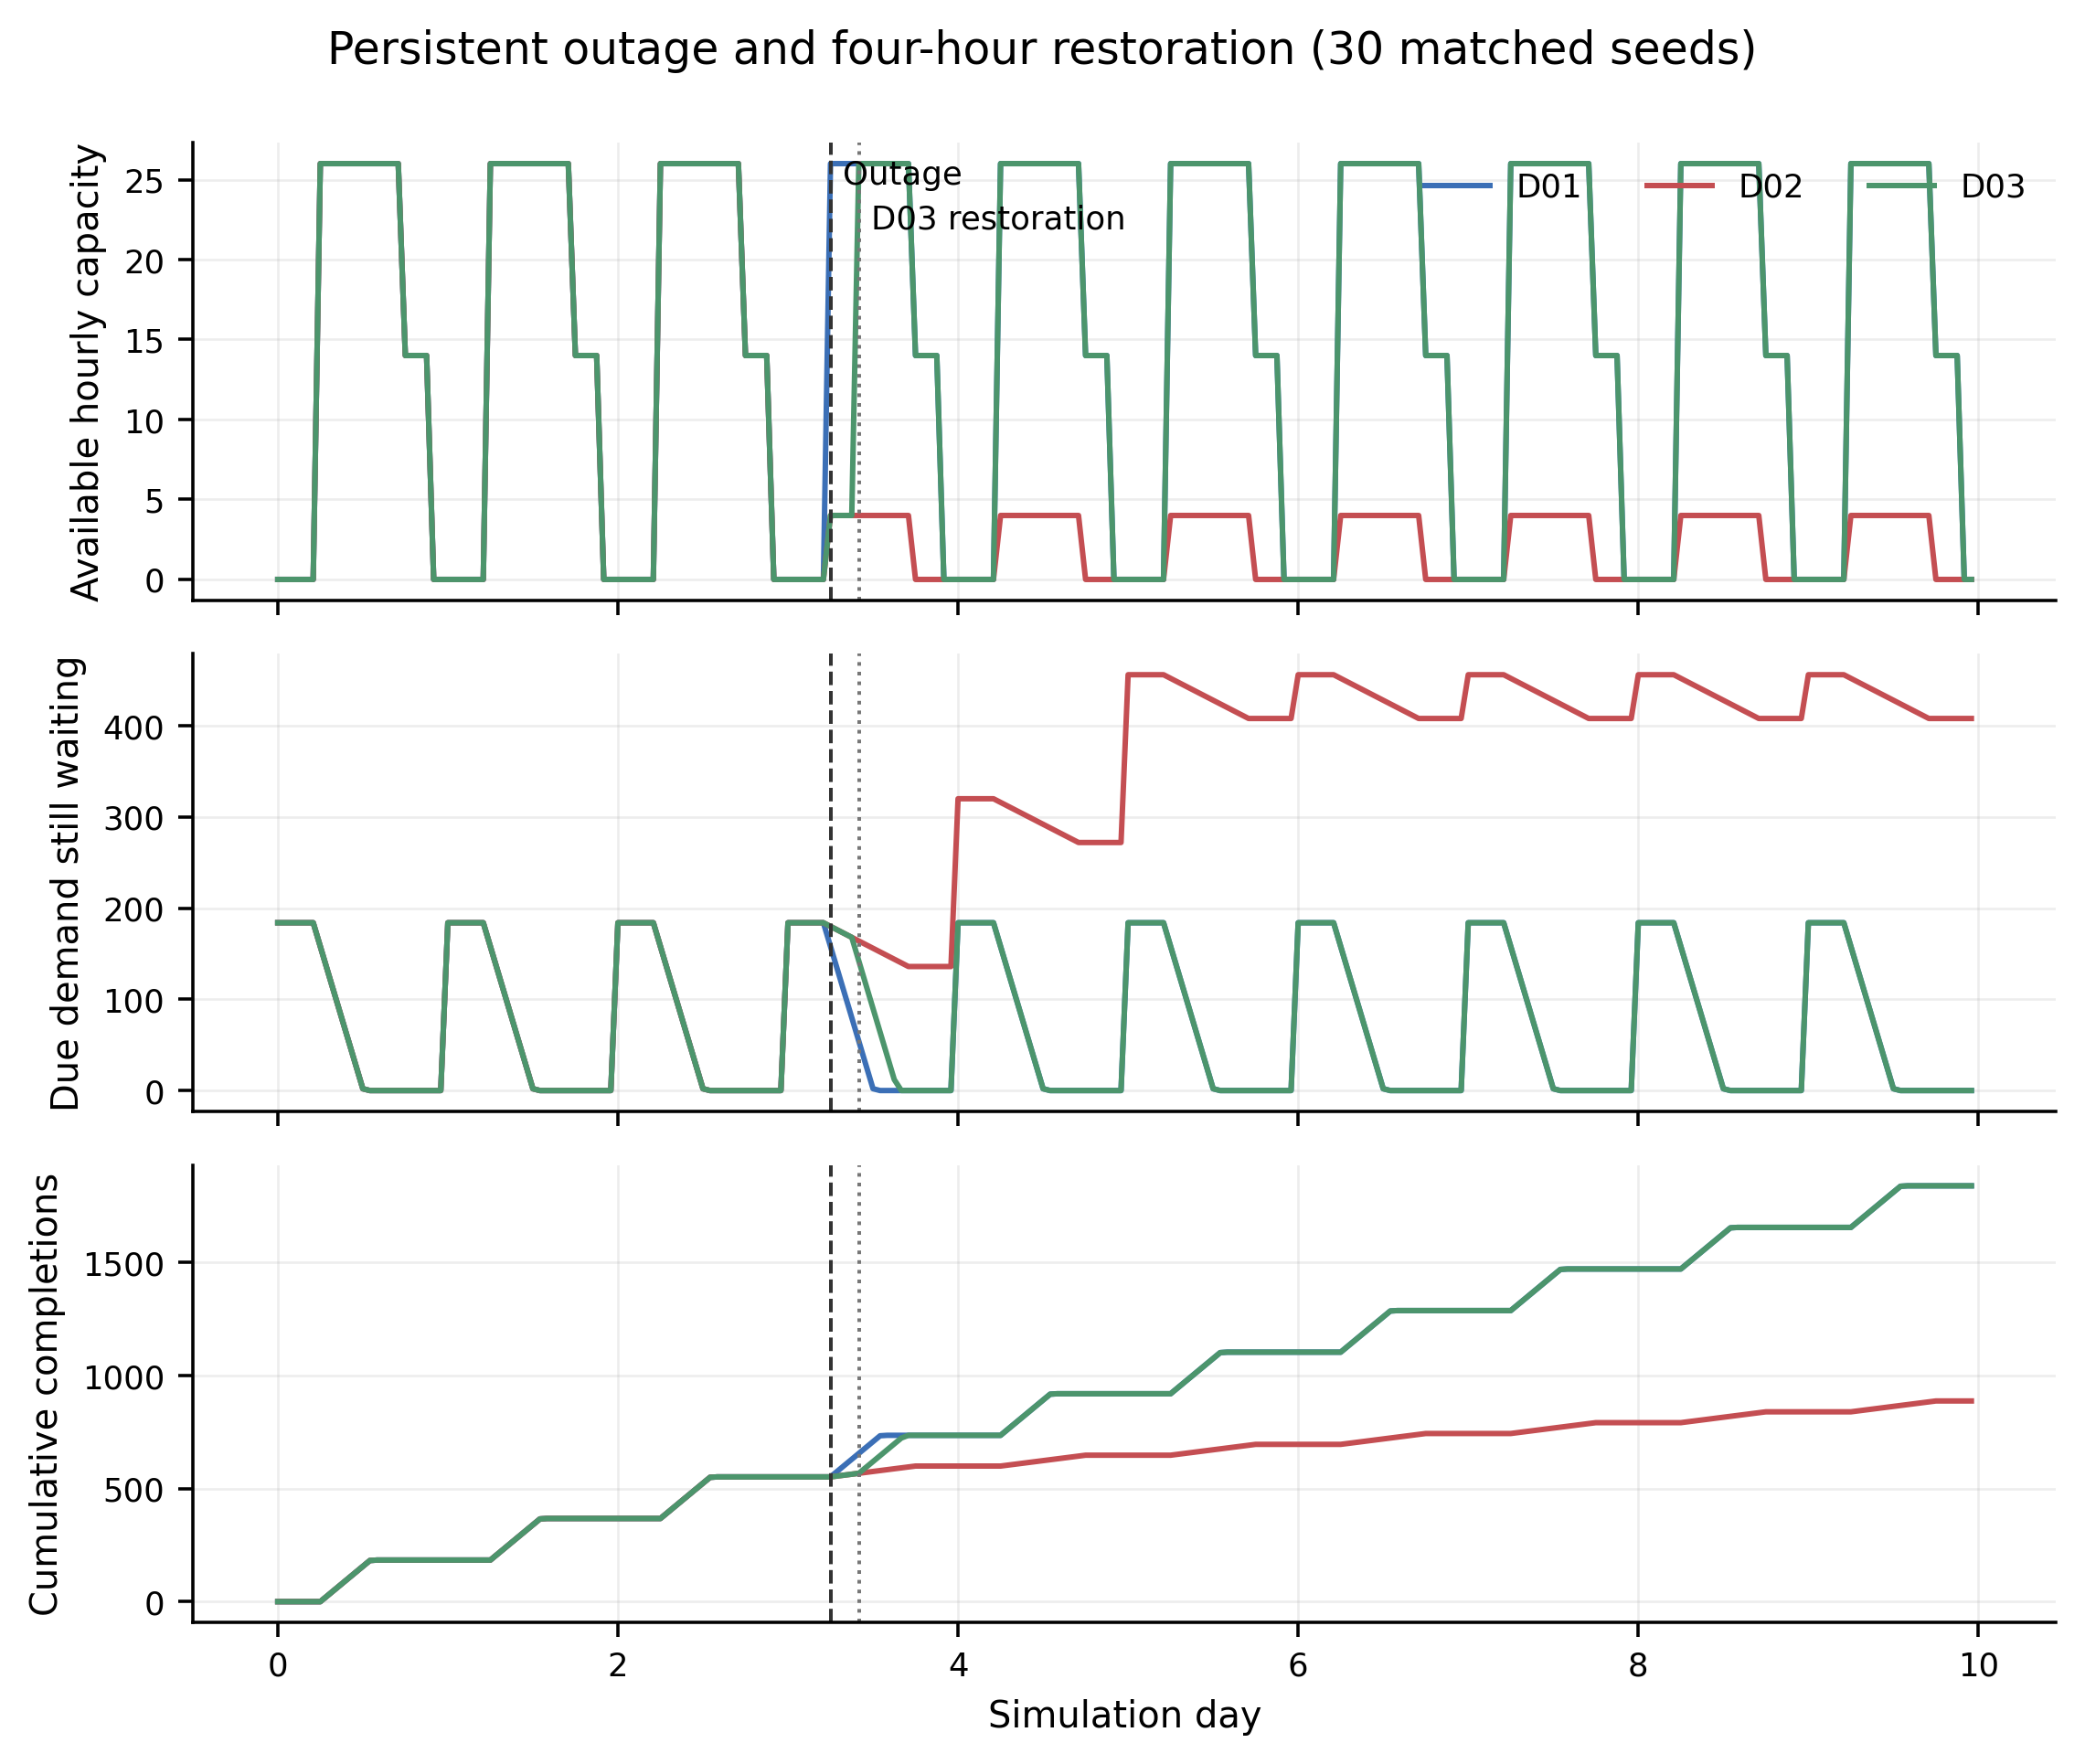
\includegraphics[width=\linewidth]
      {fig/res-health/dialysis_outage_recovery_d01_d02_d03.png}
    \caption{Mean hourly treatment response over 30 matched seeds for the reference (D01), persistent outage (D02), and temporary outage (D03) scenarios. Vertical markers identify the disruption and restoration steps.}
    \label{fig:dialysis_outage_recovery}
\end{figure}

Scenarios D04--D06 extend the comparison to flood-related and dependency disruptions. D04 applies the historical water-level series directly to the exposure thresholds of clinics and water treatment facilities. Although this produces 225 disabled clinic-hours, the network retains 100\% treatment coverage and accumulates 17,144 patient-hours of waiting, only 504 more than the D01 reference. In this configuration, the temporary facility losses can therefore be absorbed by the remaining service network within the ten-day simulation.

D05 instead applies a synthetic 10.1~m water level only to water treatment facilities, allowing clinic unavailability to propagate through the configured POI dependencies. This produces a substantially stronger effect: coverage falls to 50\%, accumulated waiting reaches 84,480 patient-hours, and an average of 552 treatment sessions remains overdue. The scenario accumulates 1,296 disabled clinic-hours.

D06 combines a scheduled ETA Moinhos outage with a synthetic 9.3~m water-level disruption and produces the same aggregate outcomes as D05: 50\% coverage, 84,480 patient-hours of waiting, 552 overdue sessions, and 1,296 disabled clinic-hours. These results show that the identical service outcomes arise through different direct mechanisms. In D05, flood blockers affect both the Menino Deus and Moinhos de Vento water sources. In D06, flooding blocks Menino Deus while the scheduled outage blocks Moinhos de Vento. In both cases, dependency conditions consequently disable all eight clinics. Thus, the infrastructure-level causes differ, but they yield the same effective clinic availability and aggregate treatment outcomes.

The complete census-sector environment provides an additional comparison at a larger spatial scale. D10 serves as its moderate reference demand and completes all due treatment sessions, with 20,700 accumulated patient-hours of waiting. Under the combined disruption in D11, coverage decreases to 71.43\%, accumulated waiting rises to 81,126 patient-hours, and an average of 415.3 sessions remains overdue. Mean admission distance also increases from 6.537~km to 7.052~km.

Across the 30 simulation run, D11 adds 60,426 patient-hours of waiting and 0.516~km to the mean admission distance relative to D10. The availability of a larger clinic network does not prevent substantial service loss under the evaluated geographically distributed disruption. This comparison should not, however, be interpreted as an isolated effect of increasing environment size, because the reduced and complete environments also differ in patient counts, clinic locations, water sources, and dependency structure.


\subsubsection{Spatial Consequences of Clinic Failure}
\label{sec:results_dialysis_spatial}

The final comparison examines whether the spatial distribution of unavailable treatment capacity affects service access. D08 and D09 remove the same nominal amount of service, 128 treatment slots per day, but distribute this loss differently across the reduced network. D08 disables one high-capacity clinic, whereas D09 disables four lower-capacity clinics.

Both scenarios maintain 100\% treatment coverage and produce the same accumulated waiting of 18,670 patient-hours. Consequently, the two failure patterns are equivalent with respect to these aggregate service outcomes under the configured demand. Their spatial effects, however, differ. Mean admission distance is 1.768~km in D08 and 2.037~km in D09, corresponding to an increase of 0.269~km when the same capacity loss is distributed across four clinics.

D09 also accumulates more disabled clinic-hours, 648 compared with 162 in D08, because the same removed capacity is distributed across a larger number of facilities. Disabled clinic-hours should therefore not be interpreted as an alternative measure of lost treatment capacity in this comparison: the scenarios intentionally remove the same nominal daily capacity but differ in the number of facilities over which that loss occurs.

The increase in mean admission distance indicates that capacity alone does not fully describe the effect of clinic loss. When multiple facilities are removed from different locations, patients who can still be treated may need to travel farther through the remaining service network. D08 and D09 therefore provide a controlled comparison in which treatment completion is preserved while the spatial cost of accessing treatment increases.


Taken together, the dialysis experiments distinguish several sources of service pressure. High demand can produce incomplete treatment without any facility becoming unavailable, while infrastructure disruptions can reduce effective service capacity even under otherwise moderate demand. Temporary and persistent failures produce substantially different outcomes, and equal nominal capacity losses can generate different travel requirements depending on which clinics become unavailable.

These results also show why dialysis-service performance cannot be characterized by coverage alone. Accumulated waiting captures delays that remain hidden when all treatments are eventually completed, overdue demand identifies sessions that cannot be recovered within the simulation horizon, and travel distance reflects the spatial consequence of redistribution across the clinic network.

The results remain conditional on the implemented service assumptions. Patients are assigned to the nearest eligible clinic with available capacity, treatment occupies one simulation step, and untreated demand is reconsidered in later hours. Appointment priorities, clinical deterioration, hospitalization, mortality, and other consequences of delayed treatment are not represented. Similarly, clinic capacities, disruption schedules, infrastructure dependencies, and synthetic water levels are scenario inputs. The experiments therefore support controlled comparisons of service behavior under the evaluated configurations rather than predictions of dialysis accessibility during an actual disruption in Porto Alegre.

\subsection{Main Findings}
\label{sec:health_results_findings}

The experiments in this section extend the mobility-oriented analyses of the preceding sections by considering scenarios in which population movement interacts with health states and access to recurring services. The epidemic experiments examine how mobility contributes to the evolution of infection across the population, whereas the dialysis experiments examine how mobility determines access to a spatially distributed and capacity-constrained healthcare network. Together, they demonstrate two complementary ways in which population movement can influence health-related outcomes.

The epidemic experiments show that changes in the configured transmission intensity substantially alter the progression of infection while preserving the same population and mobility configuration. Vaccination and reduced routine movement both decrease cumulative infections under the evaluated scenarios, and their combination produces the strongest reduction among the non-idealized intervention configurations. These results also illustrate the distinction between cumulative infection and the population simultaneously occupying the infected state, allowing different aspects of epidemic progression to be examined within the same population representation.

The dialysis experiments demonstrate that treatment access depends not only on the amount of nominal service capacity but also on when and where that capacity is available. Increasing demand progressively raises waiting even while all due treatments can still be completed, with incomplete treatment emerging once demand exceeds the configured nominal capacity. Infrastructure disruptions produce a different form of service loss: temporary outages may be absorbed by the remaining network, whereas persistent or geographically distributed disruptions can generate substantial unresolved treatment demand.

The dialysis results further show that service performance cannot be characterized by treatment coverage alone. Waiting identifies service pressure before incomplete treatment occurs, overdue sessions indicate demand that cannot be recovered within the simulation horizon, and admission distance captures changes in spatial access when patients are redistributed among available clinics. Similarly, failures removing the same nominal treatment capacity can preserve the same coverage and waiting while producing different travel requirements depending on which facilities become unavailable.

Overall, these experiments show how the population representation can support processes whose outcomes extend beyond movement itself. Mobility determines opportunities for interaction in the epidemic scenarios and access to available services in the dialysis scenarios, while additional state, capacity, and dependency constraints determine the resulting health-related outcomes. The experiments therefore complement the preceding mobility and disruption analyses by demonstrating how the same simulation framework can represent interactions between population movement, evolving individual states, recurring service demand, and infrastructure availability.
\chapter{Final Considerations}
\label{chapter:final_considerations}

%GA: resumo geral
This thesis presented LODUS, an extensible multi-scale framework for simulating heterogeneous urban populations interacting with dynamic environments. The proposed model combines an aggregated population representation with semantically defined regions and points of interest, routines and actions for changing the simulation state, and an extension mechanism through which application-specific processes can be incorporated without redefining the underlying population and environment abstractions.

%GA: tentei puxar da research question
The central research question of this thesis concerned how an extensible simulation framework could represent heterogeneous urban population dynamics at different spatial scales while supporting changes in population state, behavior, and environment availability within the same underlying model. The results indicate that LODUS provides a core representation through which these requirements can be addressed across the different application scenarios evaluated in this work. %The limitations presented in this chapter define the current scope of this representation and its experimental evaluation.



\section{Main Achievements}
\label{sec:final_discussion}


The results presented throughout this thesis support three main achievements:
the definition of an aggregated and multi-scale representation of urban populations,
the development of an extension mechanism that allows this representation to support
different population processes, and the demonstration of these capabilities across
substantially different application scenarios.

The aggregated population model represents heterogeneous populations associated
with semantically meaningful urban locations and evolving through actions and
routines. Population characteristics may either be sampled during operations or
preserved when distinctions must remain traceable throughout a simulation. This
provides a flexible compromise between representing population heterogeneity and
avoiding the computational and modeling requirements of maintaining every inhabitant
as an independent agent.

The experiments also demonstrate that the same simulation abstractions can be
instantiated at different spatial scales. Porto Alegre was represented at both
neighborhood and census-sector levels, including reduced and city-scale
census-sector environments. Although these representations differ substantially in
spatial resolution, number of locations, and represented population, they rely on
the same concepts of regions, points of interest, populations, actions, and routines.
This shows that increasing spatial detail does not require replacing the underlying
simulation structure.

The extension mechanism constitutes another central achievement of the framework.
Domain-specific plugins can introduce additional population states, points of
interest, actions, routines, dependencies, and simulation-step behavior while
preserving the underlying population and environment representation. The plugins
developed in this thesis cover routine mobility, large-scale events, environmental
disruptions, shelter demand, epidemic contagion, vaccination, and recurring dialysis
treatment. Some extensions also interact with one another, allowing, for example,
environmental conditions to affect mobility and service availability, vaccination to
modify infection dynamics, and infrastructure failures to affect access to healthcare
services.

The experimental results demonstrate the usefulness of this architecture across
substantially different population processes. The mobility experiments show that the
framework can reproduce configured recurring activity and commute patterns and
represent their spatial and temporal characteristics at different scales. Event and
flood experiments demonstrate how external conditions can alter these baseline
patterns, producing displacement, destination substitution, unmet demand, and changes
in access to urban locations. Shelter experiments further show how population
exposure can be combined with facility capacity and allocation policies to study
evacuation demand and accommodation constraints.

The health-related experiments extend the same representation beyond mobility
outcomes. Epidemic scenarios combine population movement with evolving
epidemiological states and interventions, while the dialysis scenarios combine
recurring treatment demand with clinic capacity, environmental disruption, and
infrastructure dependencies. These applications demonstrate that population movement
can serve as part of broader simulation processes in which population state and
urban-service availability evolve together.

An important achievement is also the modeling space covered by LODUS. As discussed
in Chapter~2, existing approaches address different parts of this problem through
crowd simulation, transportation simulation, human mobility models, multi-level
population representations, or general-purpose agent-based environments. However,
within the literature reviewed in this thesis, we did not identify another framework
that combines, within the same simulation architecture, dynamically aggregated
heterogeneous populations, semantically defined urban locations, multiple spatial
resolutions, changing environmental and service conditions, and extensible
domain-specific population processes. The originality of LODUS therefore lies not
in replacing these established approaches, but in integrating these capabilities
within a single population-level simulation framework.

Taken together, the experiments show that the same core abstractions can support
different spatial representations, mobility configurations, disruptions, and
application domains, while plugins define the processes acting upon the represented
population. This separation enables questions ranging from routine mobility and
environmental disruption to public health and access to essential services to be
investigated without requiring a different population simulation architecture for
each application.

Beyond the individual scenarios evaluated in this thesis, the architecture also
provides a basis for studying interactions among urban processes. Because extensions
operate over the same population and environment representation, conditions
introduced by one process can influence another. This capability is particularly
relevant to cascading scenarios in which, for example, an environmental event
simultaneously affects population mobility, shelter demand, infrastructure
availability, and access to healthcare services. The experiments presented in this
thesis therefore demonstrate not only the applicability of the implemented
extensions, but also the potential of LODUS as a foundation for integrated
population-level urban simulation.


\begin{comment}
%SO: texto do Gab
%GA: ideia de ser generalista/extensivel
The principal objective of LODUS is not to provide a specialized simulation model for a single urban phenomenon, but a common representation through which different population processes can be constructed. The experiments presented in this thesis address substantially different applications, including recurring mobility, exceptional events, environmental disruptions, evacuation, epidemic processes, and recurring healthcare services. Nevertheless, these scenarios were represented using the same underlying concepts of population blobs, points of interest, population templates, routines, actions, and environmental availability.

The population and environment abstractions provide the main basis for this reuse. Populations are represented as dynamically structured groups that can split when only part of a population is affected and merge again when their distinction is no longer required. This allows application-specific population states to be introduced without requiring every inhabitant to be represented independently. At the same time, points of interest represent more than spatial destinations: their semantic roles, attributes, availability, capacities, and dependencies can influence the population processes occurring in the simulation. Domain-specific plugins extend these common abstractions with the information and behavior required by each application rather than replacing the underlying model.

The evaluation also demonstrates the framework's multi-scale character. The same population and environment abstractions were instantiated using both neighborhood-level and census-sector-level representations of Porto Alegre. These environments differ considerably in spatial resolution and number of represented locations, but do not require distinct simulation models. The resolution can therefore be selected according to the available data and the objectives of a particular experiment while preserving the same underlying representation.

Taken together, the experiments support the central thesis claim that a common, environment-oriented, dynamically aggregated representation can be reused across different urban population phenomena without constructing an independent model for each application. The contribution of LODUS therefore lies primarily in this common representation and its extension mechanism, rather than in any individual mobility, epidemic, flood, evacuation, or healthcare model implemented for the evaluation.
\end{comment}

\section{Limitations}
\label{sec:limitations}

The proposed framework and its current implementation present limitations that
define the scope of the results reported in this thesis and identify directions for
continued development. Some of these limitations arise from deliberate modeling
choices associated with the population-level and extensible nature of LODUS, whereas
others concern capabilities that are not yet available in the current implementation.

A first limitation concerns the usability of the current implementation. LODUS
has been developed primarily as a research framework rather than as an end-user
simulation tool. Developing a new plugin currently requires programming knowledge
and familiarity with the main simulation abstractions, including populations, actions,
routines, and points of interest. Extensibility should therefore be understood primarily
as a modeling and implementation capability. Once an extension has been developed,
however, many aspects of a simulation can be configured without modifying its
implementation. The experiments presented in this thesis vary capacities, schedules,
population quantities, environmental conditions, dependencies, and behavioral
parameters through such configurations. A user-oriented authoring environment could
further separate plugin development from scenario configuration and facilitate the use
of existing extensions by non-developer users.

A second limitation concerns the representation of movement. A move action
currently transfers a population blob directly from one point of interest to another.
Distance can influence destination selection and can be recorded as an outcome, but
travel duration is not explicitly represented in the core model. Consequently, a
movement requiring several hours does not correspond to a population remaining in
transit during intermediate simulation steps. Travel time can be approximated through
domain-specific extensions, but explicit support for in-transit populations would provide
a more general solution.

Relatedly, LODUS does not aim to reproduce pedestrian locomotion, route selection,
collision avoidance, or detailed vehicle movement. Points of interest are connected at
an abstract level rather than through an explicit transportation network. This is
consistent with the intended modeling scale of LODUS, which focuses on population
distribution, demand, state changes, and movement among semantically meaningful
urban locations rather than on the detailed trajectories followed between them.
Applications requiring such detail could complement LODUS with specialized mobility
or transportation models.

The aggregated population representation introduces a related trade-off. Sampled
characteristics describe marginal distributions within a blob and do not necessarily
preserve complete joint relationships among characteristics. For example, age and
occupation distributions may both be represented without identifying how occupation
categories are distributed within each age group. Traceable characteristics allow
distinctions required by a particular simulation to be maintained, but relationships
that are absent from the input data cannot be reconstructed by the framework.
Similarly, aggregation does not preserve persistent individual identities or complete
person-level trajectories. These characteristics limit analyses that depend on individual
histories, repeated person-specific choices, or social relationships, but are consistent
with the population-level abstraction adopted by LODUS and allow large populations
to be represented without maintaining every inhabitant as an independent agent.

The empirical interpretation of the experiments must also consider the abstract and
configurable nature of the framework. LODUS itself does not define a single predictive
model for a particular urban phenomenon; rather, it provides population and environment
abstractions through which different domain-specific processes can be implemented.
Consequently, a single direct empirical validation of the framework against a real-world
ground truth is not generally applicable. The degree to which a particular LODUS
simulation reproduces real-world behavior depends on the empirical data and
domain-specific assumptions used to configure that application. In the experiments
presented in this thesis, observed and derived data were incorporated whenever
available, including population and geographic information, shelter locations and
capacities, dialysis facilities and infrastructure dependencies, and parameters associated
with epidemic processes. Other parameters were intentionally defined as experimental
conditions to enable controlled comparisons rather than calibrated predictions.

Accordingly, the results should primarily be interpreted as evaluations of whether
the framework responds consistently to the population, environmental, capacity, and
service conditions represented in each experiment. For example, the shelter experiments
evaluate how the population requiring accommodation is affected by available shelter
capacity and facility disruption, while the dialysis experiments examine how treatment
demand responds to clinic capacity and supporting-infrastructure failures. Such
experiments illustrate how LODUS can be used to explore potential consequences of
urban conditions and interventions. With sufficiently representative local data and
appropriately calibrated domain-specific extensions, the same mechanisms could support
scenario analysis and prospective studies of real-world situations. The dialysis case,
for example, illustrates how the framework can be used to investigate hypothetical
service disruptions and alternative conditions that may be difficult or undesirable to
observe experimentally in the real system.

Some application-specific extensions deliberately simplify their respective domains.
The epidemic experiments use an aggregate SIR formulation, the shelter experiments
abstract evacuation and accommodation behavior through configurable policies, and
the dialysis experiments do not model clinical consequences of delayed treatment.
These simplifications reflect the objective of evaluating the framework across distinct
population processes rather than providing fully calibrated domain-specific simulators.
More detailed applications would require corresponding domain models, data, and
validation procedures, which can be incorporated through the extension mechanism.

A further limitation is that the experimental evaluation does not include a systematic quantitative analysis of the computational performance or scalability of the framework. The experiments demonstrate LODUS with populations and environments of substantially different sizes, including city-scale census-sector representations, but execution time, memory consumption, and scaling behavior were not evaluated as experimental outcomes. Consequently, the results support the applicability of the proposed abstractions at the evaluated scales, but do not establish quantitative performance bounds or characterize how computational requirements evolve with population complexity, spatial resolution, number of points of interest, or extension behavior.

The experimental evaluation is centered on Porto Alegre and therefore does not by
itself demonstrate empirical transferability to cities with different spatial structures,
mobility patterns, service organizations, or data availability. Nevertheless, the core
LODUS representation is not specific to Porto Alegre. Regions, points of interest,
population characteristics, routines, capacities, dependencies, and environmental
conditions are instantiated from input data rather than being defined specifically for
the evaluated city. Applying LODUS to another urban environment would therefore
primarily require suitable local data and, when necessary, adaptations of
domain-specific plugins and parameters. In principle, the same framework construction
and simulation mechanisms evaluated in this thesis should remain applicable, although
their empirical adequacy would need to be assessed for the data and processes of each
new location.

Finally, the evaluation does not include a direct quantitative comparison with another
simulation framework providing the same combination of modeling capabilities. As
discussed in Chapter~2, existing approaches address different subsets of the problem,
including detailed crowd movement, transportation, human mobility, multi-level
population representation, or general-purpose agent-based simulation. We are not aware
of an existing model that provides a directly equivalent combination of dynamically
aggregated heterogeneous populations, semantically defined urban locations, multiple
spatial resolutions, dynamic environmental conditions, and extensible domain-specific
population processes. This makes a controlled state-of-the-art comparison difficult,
since differences in results would also reflect fundamentally different population,
environment, and process representations. The evaluation therefore focuses on
demonstrating the behavior, consistency, and applicability of the proposed representation
across substantially different urban population processes rather than on benchmarking
LODUS against a non-equivalent simulation model.

\begin{comment}
\section{Limitations}
\label{sec:final_limitations}

The proposed framework and its current implementation present limitations that define both the interpretation of the experiments and opportunities for continued development.

%GA: limitação de usuário
A first limitation concerns the usability of the current implementation. LODUS has been developed primarily as a research framework and is not yet intended for general end users. Developing a new plugin requires programming knowledge and familiarity with parts of the simulation model, including populations, actions, routines, and points of interest. Extensibility in the current version should therefore be understood primarily as a modeling and implementation capability rather than as an end-user authoring capability.
%GA: existe uma maneira de configurar simulações sem modelar coisas novas, mas ainda é uma limitação
There is, however, a distinction between \textit{developing} an extension and \textit{configuring} an existing one. Many of the experiments in this thesis vary capacities, schedules, population quantities, environmental conditions, dependencies, and behavioral parameters without modifying plugin behavior. Existing plugins can therefore support configurable simulation setups, although this configuration process has not yet been consolidated into a user-oriented authoring environment.

%GA: blobs "teleportam"
A second limitation concerns the representation of movement. A move action currently transfers a population blob directly from one point of interest to another. Distance can influence destination selection and be recorded as an outcome, but travel duration is not explicitly represented. A movement requiring several hours therefore does not correspond to a population remaining in transit during those intermediate simulation steps. Travel time could be approximated through domain-specific extensions, but explicit support for in-transit populations is not currently part of the core model.

%GA: cola com crowds
Relatedly, LODUS does not represent pedestrian locomotion, route selection, collision avoidance, or detailed vehicle movement. Points of interest are connected at an abstract level rather than through an explicit transportation network. The framework is therefore more appropriate for studying population distribution and movement among urban locations than for reproducing detailed trajectories between them.

%GA: limitação de joint relationships, sugerida pelo revisor do pape
The aggregated population representation also introduces limitations. Sampled characteristics describe marginal distributions within a blob and do not preserve complete joint relationships among characteristics. For example, age and occupation distributions may both be represented without identifying how occupation categories are distributed within each age group. Traceable characteristics can preserve distinctions required by a simulation, but the framework cannot reconstruct relationships that are absent from the input data.

%GA: não temos informação do individuo, o que faz parte do modelo, mas é uma limitação
Aggregation also means that LODUS does not preserve persistent individual identities or complete person-level trajectories. This is consistent with the population-level scope of the work, but limits analyses that depend on individual histories, repeated person-specific choices, social relationships, or other explicitly individual behavior.

%GA: limitação dos dados empiricos e sintéticos
A further limitation concerns parameterization and empirical validation. The experiments combine observed data, derived inputs, historical snapshots, and scenario-defined parameters. Several mobility configurations, event requests, shelter response rates, treatment capacities, disruption conditions, and interventions were selected for controlled comparisons rather than calibrated from observed behavior. Consequently, the results demonstrate the behavior of the implemented models and configurations but should not be interpreted as predictive estimates of the corresponding real-world processes.

%GA: talvez tirar abaixo
Some application-specific extensions also deliberately simplify their respective domains. The epidemic experiments use an aggregate SIR formulation, the shelter experiments abstract evacuation and accommodation behavior through configurable policies, and the dialysis experiments do not model clinical consequences of delayed treatment. These simplifications are appropriate for evaluating the framework but would require further domain-specific development for more detailed applications.

%GA: atualmente, apenas uma cidade
Finally, the evaluation is centered on Porto Alegre. The neighborhood- and census-sector-level environments demonstrate the use of different spatial representations of the same city, but do not establish transferability to cities with different spatial structures, datasets, mobility patterns, or service organizations.
\end{comment}


\section{Future Work}
\label{sec:future_work}

The limitations identified above provide several directions for future development of LODUS.

An immediate direction is a more accessible simulation-authoring process. Since existing plugins can already be configured through data and parameters, including the simulation inputs summarized in Appendix~\ref{app:input}, a user-oriented layer could expose these options through reusable simulation setups, supporting the selection of environments and extensions and the configuration of schedules, capacities, population demand, disruptions, and other scenario parameters without requiring source-code modifications.

A second direction is to extend mobility with explicit travel duration. Movements could represent populations as being in transit until a scheduled arrival determined by distance, transportation mode, a travel-time model, or routing information. This representation could subsequently support transportation networks, alternative transportation modes, and disruptions occurring between origins and destinations.

%GA: zoom
This extension also provides a possible connection with more detailed mobility and crowd models. Future work could investigate coupling LODUS with pedestrian, traffic, or agent-based simulators when selected locations or periods require greater detail. Populations could remain aggregated at the urban scale while more detailed representations are used only where required by the simulation.

%The population representation could also be extended with joint or conditional distributions when suitable data are available, preserving relationships among characteristics such as age, occupation, health status, or transportation mode.

Further work should also address empirical calibration and validation. Mobility behavior could be compared with origin--destination surveys, transportation records, or other observational datasets, while domain-specific extensions could be evaluated against corresponding service or population data. Applying the framework to additional cities would also help evaluate how well the core abstractions transfer to different urban structures and data sources.

The environmental representation provides additional opportunities for studying interconnected urban services. The dependency mechanism evaluated with dialysis clinics and water-treatment facilities could be expanded to include electricity, transportation, communications, healthcare, shelters, and other infrastructure, supporting scenarios in which disruptions propagate through multiple services.

Domain-specific extensions may similarly incorporate additional detail when required, while keeping such behavior within the corresponding plugins rather than introducing it as a requirement of the core model.

%GA: ideia de digital shadow
Finally, future work could investigate stronger integration with dynamic and data-driven inputs. Environmental observations could update simulation conditions during execution, while statistically calibrated or learned models could provide destination choices, activity demand, service use, or responses to disruptions. LODUS would continue to provide the core population and environment representation through which these processes interact.


\section{Published Papers}
\label{sec:published_papers}

During the doctoral period, the author participated in publications addressing crowd simulation, virtual humans, simulation authoring and visualization, generative models, and urban population simulation. Table~\ref{tbl:thesis_publications} summarizes these publications and their main research topics. Among them, the LodusPop publication~\cite{silva2026lodusPop} is directly associated with the framework developed and evaluated in this thesis.

\begin{table}[ht]
    \centering
    \footnotesize
    \setlength{\tabcolsep}{4pt}
    \caption{Publications produced during the doctoral period.}
    \label{tbl:thesis_publications}
    \begin{tabularx}{\linewidth}{@{}p{4.9cm}p{2.6cm}p{0.8cm}X@{}}
        \toprule
        \textbf{Publication} &
        \textbf{Venue} &
        \textbf{Year} &
        \textbf{Topic} \\
        \midrule

        \textit{Perception of Personality Traits in Crowds of Virtual Humans}~\cite{nardino2021perception}
        & SBGames
        & 2021
        & Perception of personality traits and behavioral differences in crowds of virtual humans. \\

        \textit{WebCrowds: An Authoring Tool for Crowd Simulation}~\cite{silva2022webcrowds}
        & SBGames
        & 2022
        & Authoring and configuration of crowd-simulation scenarios through an interactive tool. \\

        \textit{Evaluating and Comparing Crowd Simulations: Perspectives from a Crowd Authoring Tool}~\cite{silva2024evaluating}
        & Graphical Models
        & 2024
        & Evaluation and comparison of crowd-simulation configurations using quantitative measures and visualization. \\

        \textit{Exploring Foundation Models for Synthetic Medical Imaging: A Study on Chest X-Rays and Fine-Tuning Techniques}~\cite{dasilva2024foundation}
        & SIBGRAPI
        & 2024
        & Use of foundation and generative models for synthetic medical imaging and chest X-ray generation. \\

        \textit{Visualization of Crowd Contamination Simulations Using Immersive Virtual Reality}~\cite{teixeira2024visualization}
        & IEEE COMPSAC
        & 2024
        & Immersive visualization and exploration of crowd-contamination simulation results. \\

        \textit{Surveying the Evolution of Virtual Humans Expressiveness toward Real Humans}~\cite{knob2024surveying}
        & Computers \& Graphics
        & 2024
        & Survey of the evolution of expressiveness and realism in virtual humans. \\

        \textit{Evaluating the Gender Label in Virtual Babies Using an Interactive Environment}~\cite{araujo2025gender}
        & ACM IVA
        & 2025
        & Perception of gender labels and visual characteristics in interactive virtual-human representations. \\

        \textit{LodusPop: an Environment-Driven Multi-Scale Simulation Framework for Urban Population Dynamics}~\cite{silva2026lodusPop}
        & The Visual Computer
        & 2026
        & Environment-driven and multi-scale simulation of urban population dynamics. This publication is directly associated with the framework developed in this thesis. \\

        \bottomrule
    \end{tabularx}
\end{table}


\section{Closing Remarks}
\label{sec:final_closing}

Urban population dynamics emerge from the interaction of populations with locations, services, infrastructure, and changing environmental conditions. Representing these processes does not always require maintaining every inhabitant independently, particularly when available data and the questions being investigated concern population-level behavior.

LODUS provides a core representation for studying these interactions through heterogeneous aggregated populations and dynamic urban environments. The experiments presented in this thesis demonstrate that this representation can be instantiated at different spatial resolutions and extended to address distinct population processes without redefining its underlying model. The limitations and future directions identified in this chapter provide opportunities to further expand its accessibility, mobility representation, population description, empirical validation, and application to other urban environments.

%\include{_5c-environment-disruptions}
%\include{_5d-results_dialysis}
%\chapter{Visualization and Exploratory Analysis}
\label{sec:visualization}

Simulation output is only useful when its spatial, temporal, and population dimensions can be inspected without obscuring the assumptions that generated it. LodusPop produces several complementary forms of output: node occupancy and population state over time, movement events between origins and destinations, effective node availability and its direct or dependency-derived causes, and domain-specific records such as admissions, queues, unmet demand, and rerouted visits. These records can support visual analysis at different levels of aggregation, but a visualization does not validate the simulation that produced them. It provides an interface for examining results, detecting anomalies, comparing scenarios, and communicating patterns that must still be interpreted with reference to the model, data provenance, and validation evidence.

This chapter examines two visualization approaches developed in connection with LODUS and LodusPop. The first uses immersive virtual reality to place temporal occupancy and displacement data in a three-dimensional urban environment~\cite{teixeira2024visualization}. The second is a browser-based tool for exploring aggregate origin--destination flows at multiple geographic levels~\cite{silva2026geospatial}. They operate on related movement data but answer different analytical questions. The immersive application emphasizes temporal inspection and interaction with places of interest; the geographic-flow tool emphasizes relationships between territorial units, multiscale aggregation, demographic filtering, and coordinated statistical views.

\section{Historical Context: Legacy Multi-Resolution Views}
\label{visualization:legacy}

The original LodusPop discussion used Unity renderings to illustrate how the same simulated environment could be viewed at different spatial levels. Figure~\ref{fig:legacy_multiresolution} shows a detailed urban representation with one area highlighted and a broader view in which abstract population blobs are distributed across the city. These images remain useful as historical context: they communicate the intended relationship between geographic detail and abstract population state. They should not, however, be presented as an evaluation of either visualization system discussed below. They predate the current visualization studies, do not expose an analytical task or evaluation protocol, and are not screenshots of the immersive prototype described by Teixeira et al.~\cite{teixeira2024visualization} or of the geographic-flow tool~\cite{silva2026geospatial}.

\begin{figure}[!htb]
  \centering
  \begin{subfigure}{0.48\textwidth}
    \centering
    \includegraphics[width=\linewidth]{fig/results/Lodus1.png}
    \caption{Detailed urban representation with a region of interest highlighted.}
    \label{fig:visualization_region}
  \end{subfigure}
  \begin{subfigure}{0.48\textwidth}
    \centering
    \includegraphics[width=\linewidth]{fig/results/Lodus2.png}
    \caption{Abstract population blobs shown across a broader urban environment.}
    \label{fig:visualization_blob}
  \end{subfigure}
  \caption{Legacy Unity renderings used in the original LodusPop multi-resolution discussion. The images illustrate alternative spatial views of a simulated environment; they are contextual illustrations rather than evidence of visualization effectiveness.}
  \label{fig:legacy_multiresolution}
\end{figure}

For this reason, the legacy material is retained as a single transitional figure rather than as a separate experimental result. The substantive evidence and limitations of the two visualization artifacts are reported in the following sections.

\section{Immersive Virtual-Reality Visualization}
\label{visualization:vr}

Teixeira et al.~\cite{teixeira2024visualization} developed an immersive prototype for inspecting crowd contamination simulations in an urban environment. The application was implemented in Unity3D for the Meta Quest~2. Its objective was to examine whether simulation records describing occupancy, capacity, and population displacement could be placed in an interactive three-dimensional map rather than being restricted to a desktop dashboard.

The prototype separates the geographic environment from the simulation events. It receives three inputs: an OpenStreetMap file describing roads and buildings; a file identifying the regions and points of interest to be monitored, including their coordinates, type, and configured capacity; and a formatted simulation-event file describing population states and displacement events over discrete simulation steps. This separation allows a subset of locations to be selected for visualization without regenerating the simulation. Routes between origins and destinations are requested through the Open Source Routing Machine~\footnote{Open Source Routing Machine: ~\url{https://project-osrm.org/}} and retained for subsequent events. Figure~\ref{fig:vr_pipeline} presents and overview of the pipeline and the resulting interface.

\begin{figure}[ht]
    \centering
    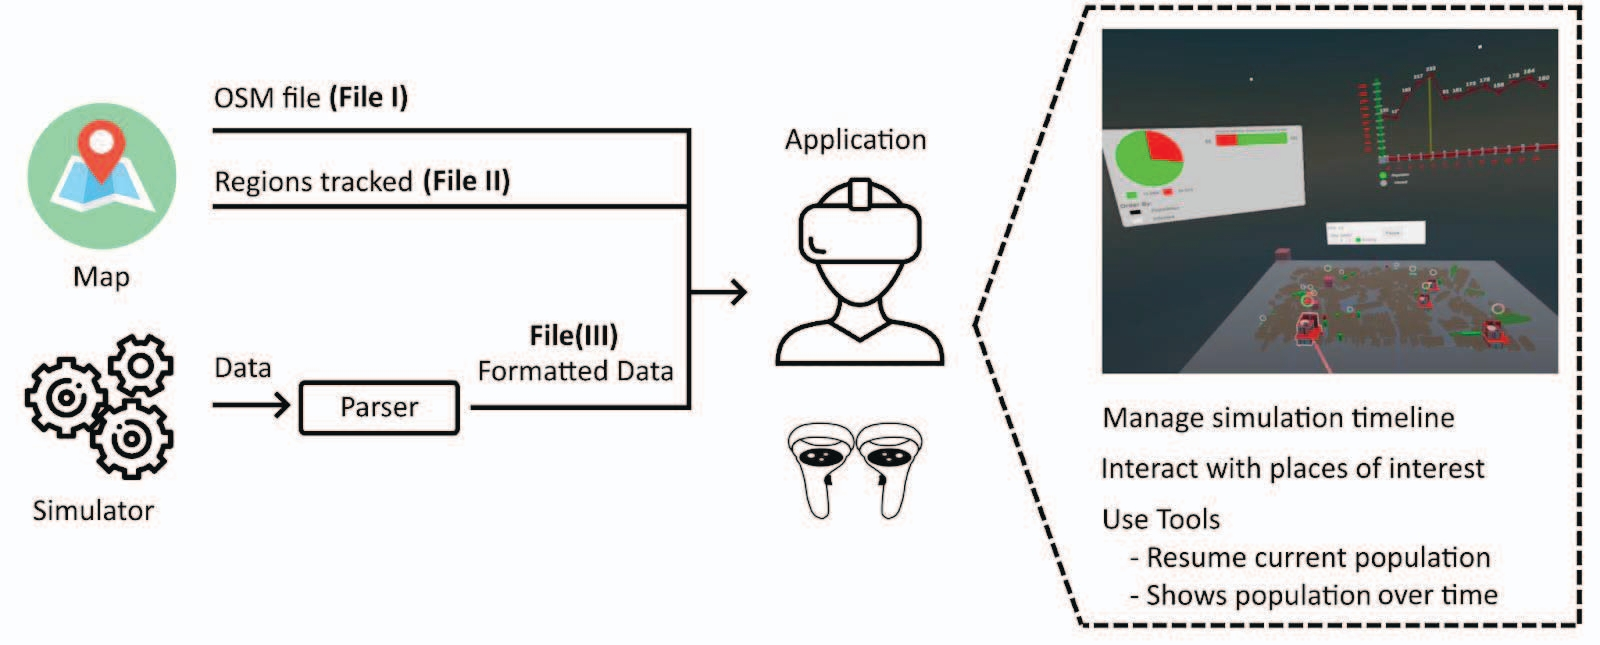
\includegraphics[width=0.98\linewidth]{fig/viz/vr_application_overview.jpg}
    % TODO: confirm the publisher-required IEEE copyright credit line before final submission.
    \caption{Overview of the immersive application: map, monitored points of interest, and formatted simulation data are combined in a Unity application in which the user controls time, interacts with places of interest, and inspects population summaries. Reproduced from Teixeira et al.~\cite{teixeira2024visualization}.}
    \label{fig:vr_pipeline}
\end{figure}

The application reconstructs roads, buildings, and green areas from OpenStreetMap data and instantiates a distinct three-dimensional model for each monitored point of interest. A circular indicator communicates the relation between current occupancy and configured capacity; a warning is shown when the capacity is reached, and the building model increases in size as occupancy grows. These behaviors make changes at monitored locations visible in their geographic context.

Users navigate the discrete simulation steps through a clock-shaped controller that supports forward and backward movement. A two-dimensional control panel starts the visualization, changes animation speed, and can hide points of interest that are not part of the monitored set. A line chart displays occupancy over time for selected buildings, while a monitor reports their current population. Locations can be selected individually with the controller or collectively with a three-dimensional selection volume. Figure~\ref{fig:vr_scene} presents the main components of the immersive scene.

\begin{figure}[ht]
    \centering
    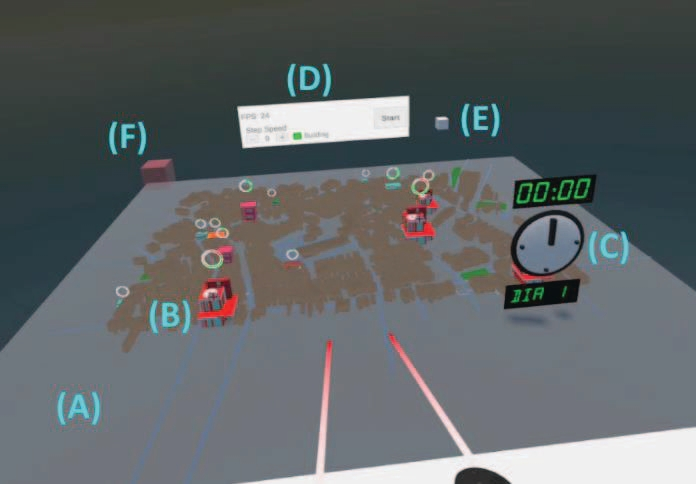
\includegraphics[width=0.72\linewidth]{fig/viz/vr_scene_elements.jpg}
    % TODO: confirm the publisher-required IEEE copyright credit line before final submission.
    \caption{Main elements of the immersive scene: the three-dimensional map and monitored establishments, simulation controls, temporal chart, and spatial selection tool. Reproduced from Teixeira et al.~\cite{teixeira2024visualization}.}
    \label{fig:vr_scene}
\end{figure}

Displacement events are animated as groups of cylinders moving between the source and destination. Green cylinders represent healthy population and red cylinders represent infected population. The model explicitly treats this movement as illustrative: cylinder speed is randomized, and the animation communicates that a transfer occurred rather than reconstructing the trajectories of simulated individuals.

The published demonstration used 13 points of interest in the Independ\^encia neighborhood of Porto Alegre, seven simulation steps, and randomly generated displacement and infection events\footnote{A video demonstration is available at: \url{https://www.youtube.com/watch?v=l2gKNdp22JM}}. It shows that the prototype could load the files, construct the scene, animate transfers, select establishments, and update occupancy summaries.

Still, the tool does not validate a hospital-demand process, infection model, capacity policy, or emergency intervention. The population, displacement, and contamination events were synthetic, and the study did not compare the displayed values with observed clinical or mobility data. Therefore, this work treats the prototype as a visualization contribution and a possible inspection interface, not as validation of LodusPop.

\section{Interactive Geographic Flow Visualization}
\label{visualization:od}

The geographic-flow tool developed by Silva~\cite{silva2026geospatial} addresses a different unit of analysis: aggregate flows between territorial units. Its minimum input is an origin--destination matrix containing an origin code, destination code, and movement count. Optional names and demographic tables improve labeling and filtering. Geographic boundaries, representative points or centroids, and lookup tables connect base units to more aggregated territorial levels. The preprocessing pipeline standardizes the inputs, converts boundaries to WGS~84, produces GeoJSON and centroid files, and stores flow tables in the columnar Parquet format.

The application is implemented with React and TypeScript, uses MapLibre for interactive geographic layers, and executes analytical queries in the browser through DuckDB-WASM. Dataset-specific JSON profiles define file locations, geographic levels, labels, demographic dimensions, filters, and available charts. IndexedDB provides local persistence for auxiliary data, profiles, and imported simulations. Separating the data artifacts, configuration, and interface logic allows the same application to be reused without encoding one city's names or geographic hierarchy directly in its components.

The browser architecture reduces dependence on a dedicated database server, but it does not remove resource limits. Query and rendering cost depend on the number of flow records, aggregations, and visible lines, while WebAssembly and browser memory constrain the size of datasets that can be processed locally. Large or dense matrices may require partitioning, pre-aggregation, column reduction, or server-side processing.

\subsection{Interactive and Multiscale Exploration}

The interface is centered on a map in which flows are drawn as lines between representative points of the origin and destination areas. Color and thickness encode flow magnitude. The user selects a territorial unit and then explores incoming or outgoing connections rather than displaying the entire matrix at once. Controls limit the maximum number of visible lines and suppress connections below a chosen count, reducing visual clutter without altering the underlying records.

The interface combines six functional areas: selection of the active dataset; definition of the geographic level, selected area, direction, and demographic filters; a summary of the current selection; density controls; the geographic map; and a coordinated analytical panel. The panel reports quantities such as leading connections, demographic composition, origin--destination heat maps, and directional balance. Selections in charts can filter the other views, supporting coordinated exploration of spatial and demographic patterns. Figure~\ref{fig:od_interface} presents the main interface.

\begin{figure}[ht]
    \centering
    \includegraphics[width=0.98\linewidth]{\vizfigpath/od_interface_overview.png}
    \caption{Interactive geographic-flow interface, including dataset and area selection, summary and density controls, the flow map, and coordinated analytical views. Reproduced from the student-led geographic-flow study~\cite{silva2026geospatial}.}
    \label{fig:od_interface}
\end{figure}

Multiscale exploration is implemented by mapping base units to an aggregated geography. In the principal dataset, the base units are Middle Layer Super Output Areas (MSOAs), which can be aggregated to Lower Tier Local Authorities (LTLAs). In the Porto Alegre configuration, census sectors are the base units and neighborhoods are the aggregate units. Figure~\ref{fig:od_multiscale} illustrates the trade-off. The detailed MSOA view exposes local structure but produces a denser display; the LTLA view emphasizes broader regional connections with less visual clutter. Aggregation changes the analytical unit and can hide within-area variation, so the two views should be interpreted as complementary rather than interchangeable.

\begin{figure}[ht]
    \centering
    \subfloat[Incoming flows at the more detailed MSOA level.]{
        \includegraphics[width=0.48\linewidth]{\vizfigpath/od_flows_msoa.png}
    }
    \hfill
    \subfloat[The corresponding type of exploration at the aggregated LTLA level.]{
        \includegraphics[width=0.48\linewidth]{\vizfigpath/od_flows_ltla.png}
    }
    \caption{Origin--destination flows at two geographic levels. The detailed view preserves more local relations, while aggregation supports recognition of regional patterns. Reproduced from Silva~\cite{silva2026geospatial}.}
    \label{fig:od_multiscale}
\end{figure}

The flow lines connect representative points and do not show the roads or routes actually traveled. They should therefore be read as spatial relationships between areas. An apparent line across the map is not evidence that a traveler followed that geometry, and overlapping lines may conceal variation when an area has many connections. The intensity map and analytical charts offer complementary summaries when pairwise lines become too dense.

\subsection{Evaluation, Reuse, and Limitations}

The principal evaluation uses official 2021 census commuting data for England and Wales, including social-class and age dimensions. A simulated Porto Alegre matrix uses census sectors and neighborhoods with age and occupation categories. The Porto Alegre values are synthetic and serve to test adaptation to another geography and configuration; they are not evidence about observed mobility in the city.

The performance evaluation is exploratory. Twenty LTLA selections produced an overall median latency of 373~ms, a minimum observed value of 150~ms, and a final recorded value of 543~ms. Nine queries classified as DuckDB-WASM without a warmed cache had a median of 180~ms, whereas eleven queries classified as using a warmed cache had a median of 586~ms. Because these groups did not repeat the same areas, filters, directions, and connection counts, the difference cannot be interpreted as evidence that caching increases latency. A controlled evaluation would repeat equivalent queries before and after cache warming and separately measure data access, aggregation, geographic conversion, and rendering.

The tool also supports the interactive application of a replacement origin--destination matrix to an already configured geography. The user maps origin, destination, and count columns, may attach demographic dimensions, and can apply, save, or restore the matrix. Figure~\ref{fig:od_custom_matrix} shows this workflow. It is directly relevant to simulation reuse because a new LodusPop result can be inspected without redefining boundaries and centroids when the geographic identifiers already match a configured dataset.

\begin{figure}[ht]
    \centering
    \includegraphics[width=0.75\linewidth]{\vizfigpath/od_custom_matrix.png}
    \caption{Interface for applying a custom origin--destination matrix: base-flow upload and column mapping, optional demographic dimensions, and actions for applying, saving, or restoring the matrix. Reproduced from Silva~\cite{silva2026geospatial}.}
    \label{fig:od_custom_matrix}
\end{figure}

The study demonstrates a functional pipeline, multiscale interaction, configurable reuse, and initial browser performance. It does not include a controlled user study, comparison with alternative flow visualizations, or a completed analytical evaluation using the recent dialysis, inpatient, Popular Times, or commuting batches. Its strongest supported claim is therefore that the application can ingest and interactively explore compatible aggregate flow data across more than one geographic configuration.

\section{Relationship to the Recent LodusPop Experiments}
\label{visualization:recent}

The recent experiments produce several relationships that can be transformed into origin--destination matrices: home--clinic admissions in dialysis, origin--hospital admissions in inpatient care, home--POI activity visits in Popular Times, and home--work or home--school movements in Levy Walk V2. Scenario, seed, time, population category, destination state, and movement outcome can be retained as dimensions or used to generate separate matrices. The geographic-flow tool is therefore well suited to questions such as which origins lose access after a disruption, which facilities receive displaced demand, and whether rerouting concentrates additional load in a small number of destinations.

That integration has not yet been evaluated as part of the reported experiment batches. Producing a compatible matrix is technically supported by the movement and domain loggers, and the custom-matrix interface supports reuse of an existing geography, but a complete study would still need an explicit export specification, reproducible transformation scripts, analytical tasks, and verification that filtered totals agree with the source logs. Temporal changes may require matrices per interval or a time dimension not emphasized in the current OD evaluation.

The immersive prototype could represent the same transfers as animated events and could associate occupancy or capacity values with hospitals and clinics. Current LodusPop outputs would nevertheless require an adapter, and new visual encodings would be necessary for effective availability, independent disable causes, dependency failure, queues, unmet demand, and rerouting. Until such an integration is implemented and evaluated, these uses remain prospective.

\section{Interpretive Role and Author Contributions}
\label{visualization:contribution}

The two artifacts complement rather than replace the numerical analyses. Immersive views preserve a sense of urban context and temporal change at selected establishments. Geographic-flow views support comparison of origins, destinations, territorial scales, demographic categories, and redistributed demand. Both can expose anomalies or suggest follow-up questions, but neither determines whether the simulated behavior is realistic. A visually coherent flow can still originate from a synthetic demand assumption, and an apparently plausible animation does not provide calibration evidence.

The immersive prototype is collaborative published work by Teixeira, the thesis author, and their coauthors~\cite{teixeira2024visualization}. The geographic-flow application and manuscript are student-led work developed by Gustavo Willian Martins da Silva under the thesis author's supervision~\cite{silva2026geospatial}. The contribution of this thesis chapter is to relate these artifacts to the LodusPop output model, distinguish demonstrated functionality from prospective integration, and define the evidential limits under which their visualizations should be interpreted.

Future evaluation should use representative tasks and intended users. Measures should include accuracy, completion time, insight quality, confidence, and usability. Comparisons should isolate immersion from interaction design and compare multiscale flow views with appropriate tabular or geographic baselines. Visual evaluation should remain separate from simulation validation.

\begin{table}[ht]
    \centering
    \footnotesize
    \caption{Complementary roles of the visualization artifacts.}
    \label{tbl:visualization_comparison}
    \begin{tabularx}{\linewidth}{@{}lXX@{}}
        \toprule
        \textbf{Dimension} & \textbf{Immersive VR prototype} & \textbf{Geographic-flow tool} \\ \midrule
        Primary representation & Three-dimensional urban scene, monitored establishments, temporal occupancy, and animated transfers & Aggregate origin--destination relations, territorial boundaries, intensity layers, and coordinated charts \\ \midrule
        Principal interaction & Timeline control, pointing, individual or volume-based location selection, and occupancy inspection & Area and dataset selection, incoming/outgoing direction, geographic aggregation, demographic filters, and density controls \\ \midrule
        Published demonstration & 13 monitored locations, seven frames, and synthetic displacement and infection events & England and Wales census commuting as the principal dataset; simulated Porto Alegre data as a portability case \\ \midrule
        Strongest supported claim & Feasibility of loading and interactively presenting the prototype's simulation format in VR & Feasibility of configurable, browser-based, multiscale exploration of compatible aggregate flows \\ \midrule
        Main limitation & No controlled user study or behavioral/clinical validation; movement animation is illustrative & Centroid lines are not routes; performance study is exploratory; no controlled user study \\ \midrule
        Status for recent experiments & Prospective; requires an export adapter and additional state encodings & Compatible export is supported, but the recent batches have not been formally evaluated in the tool \\ \bottomrule
    \end{tabularx}
\end{table}
%================================================================
% Aqui vai a bibliografia. Existem três estilos de citação: use
% 'ppgcc-alpha' para citações do tipo [Abc+] ou [XYZ] (em ordem
% alfabética na bibliografia), 'ppgcc-num' para citações
% numéricas do tipo [1], [20], etc., por ordem de citação, OU
% 'ppgcc-apalike' para citações do tipo "(Silva F., 2019) e 
% Silva F., (2019)".
%
%----------------------------------------------------------------
% NUMÉRICO:
\bibliographystyle{ppgcc-num}
%----------------------------------------------------------------
% ALPHA:
%\bibliographystyle{ppgcc-alpha}
%----------------------------------------------------------------
% APALIKE: 
% !!! Lembrar de fazer uso do pacote 'natbib'. Linha 70 !!!
% Funcionando em ambos os modos 'portuguese' e 'english'.
% Prefira esse (ppgcc-apalike) no lugar de somente 'apalike':
%\bibliographystyle{ppgcc-apalike}
%----------------------------------------------------------------
% !!! DICA APALIKE !!!:
% "Recomendamos o uso de dois estilos diferentes de citações para
% o APALIKE: 'citep' e 'citet'. O \citep traz os nomes dos autores 
% e também o ano para a referência, tudo entre parênteses 
% (utilizado nos finais de parágrafos). Enquanto que o '\citet' 
% atua como uma referência interna ao texto, por exemplo: 
% "De acordo com~\citet{borges:2020} o tema..." (deixando apenas 
% o ano entre parênteses e o nome dos autores fora dos parênteses). % E para as fontes de livros, os números das páginas 
% (opcionalmente) podem ser exibidos usando colchetes, com números 
% de páginas, como neste exemplo: 
% ~\citep[10-100]{CORMEMALGORITHMS01}."

%================================================================
% Arquivo que consta as referências (.BIB)
\bibliography{bib}

%================================================================
% Após \appendix, se iniciam os capítulos de Apêndice, com
% numeração alfabética.
%----------------------------------------------------------------
\appendix
\chapter{Input and Simulation Setup}
\label{app:input}

This appendix illustrates how the elements defined in Chapter~\ref{chapter:proposed_model} can be represented when preparing a LODUS simulation. A simulation setup comprises: 
\begin{itemize} 
    \item \textit{i)} environment data describing regions, points of interest, their attributes, and dependency requirements (Section~\ref{app:input_environment}); 
    \item \textit{ii)} population data describing the initial blobs and their sampled and traceable characteristics (Section~\ref{app:input_population}); 
    \item \textit{iii)} routine data describing local and global scheduled actions (Section~\ref{app:input_routine}); 
    \item \textit{iv)} an experiment configuration defining the simulation horizon, selected plugins, and their parameters (Section~\ref{app:experiment_configuration}); and 
    \item \textit{v)} the simulation procedure that combines these elements and advances the simulation over time (Section~\ref{app:simulator}). 
\end{itemize} 

The examples are deliberately small and illustrate how the abstractions of the proposed model can be instantiated for a simulation. The specific data sources and attributes depend on the application domain, while the representation of regions, points of interest, blobs, templates, routines, and actions follows the definitions introduced in Chapter~\ref{chapter:proposed_model}.


\section{Environment Input Files}
\label{app:input_environment}

The environment input represents the regions $R$ and points of interest $P$ defined in Section~\ref{sec:environment}. A region is identified by a name, a reference coordinate, and a collection of points of interest. Each point of interest has an identifier, a semantic type corresponding to $\tau_i$, a coordinate, and an optional collection of attributes corresponding to $\bm{\alpha}_i$.

Listing~\ref{lst:environment_description} illustrates an environment containing a home, a school, a pharmacy, and infrastructure points of interest. The attributes associated with each point of interest represent properties that may be relevant to the corresponding experiment. For example, a capacity may be used in a service scenario, while a water-level threshold may be used in a flood scenario. Their interpretation depends on the behavior defined for the experiment.

\begin{lstlisting}[language={Python},
caption={Example of an environment input file with typed POIs and attributes.},
captionpos=b, label={lst:environment_description}, basicstyle=\scriptsize]
{
  "regions": [
    {
      "name": "ExampleRegion",
      "lng_lat": [-51.19757, -30.15647],
      "points_of_interest": [
        {
          "poi_type": "home",
          "unique_name": "home_0",
          "lng_lat": [-51.19805, -30.15633],
          "attributes": {"external_id": "H-001"}
        },
        {
          "poi_type": "school",
          "unique_name": "school_0",
          "lng_lat": [-51.19750, -30.15621],
          "attributes": {"capacity": 120}
        },
        {
          "poi_type": "pharmacy",
          "unique_name": "pharmacy_0",
          "lng_lat": [-51.19820, -30.15655],
          "attributes": {"capacity": 40, "water_level": 3.5}
        },
        {
          "poi_type": "power_source",
          "unique_name": "power_source_0",
          "lng_lat": [-51.19910, -30.15590]
        },
        {
          "poi_type": "water_source",
          "unique_name": "water_source_0",
          "lng_lat": [-51.19940, -30.15560]
        },
        {
          "poi_type": "water_source",
          "unique_name": "water_source_1",
          "lng_lat": [-51.19680, -30.15570]
        }
      ]
    }
  ]
}
\end{lstlisting}

The direct disabling conditions $\bm{C}_i(t)$ represent simulation state and therefore do not need to be specified as permanent availability values in the environment description. Such conditions may be introduced or removed during the simulation, for example when a point of interest closes or becomes exposed to flooding.

Dependency requirements $D_i$ may also be supplied as part of the environment configuration. As defined in Section~\ref{sec:environment}, each requirement is represented by a pair $(k_{ir},\bm{G}_{ir})$, where $\bm{G}_{ir}$ contains a set of prerequisite points of interest and $k_{ir}$ specifies the minimum number that must be available.

For example, the pharmacy introduced in Listing~\ref{lst:environment_description} may require an available power source and at least one of two available water sources. These requirements correspond to

\[ D_p = \left\{ (1,\{P_e\}), (1,\{P_{w_1},P_{w_2}\}) \right\}. \] 

The first requirement represents a mandatory dependency on $P_e$, while the second allows either $P_{w_1}$ or $P_{w_2}$ to satisfy the water dependency. All requirements contained in $D_p$ must be satisfied for the pharmacy to be available. 

Changes in availability do not directly modify the population occupying a point of interest. Any cancellation, waiting, movement, or redirection of that population is expressed through the actions and domain-specific behavior defined for the simulation.

\begin{lstlisting}[language={Python},
caption={Example of all-of and minimum-of POI dependency rules.},
captionpos=b, label={lst:dependency_description}, basicstyle=\scriptsize]
{
  "dependency_rules": {
    "pharmacy_infrastructure": {
      "all_of": [
        "ExampleRegion//power_source_0"
      ],
      "min_of": [
        {
          "minimum_enabled": 1,
          "nodes": [
            "ExampleRegion//water_source_0",
            "ExampleRegion//water_source_1"
          ]
        }
      ]
    }
  },
  "node_dependencies": {
    "ExampleRegion//pharmacy_0": ["pharmacy_infrastructure"]
  }
}
\end{lstlisting}

The simulator recomputes effective availability after a direct state change
and propagates dependency effects until the states stabilize. Unavailability
does not itself move, delete, or queue a blob. The handler consuming an action
must explicitly decide whether to suppress, retain, redirect, or otherwise
transform the affected demand.


\section{Population Input Files}
\label{app:input_population}

The population input describes the initial blobs $B=(TP,\bm{Tc},\bm{Sc})$ defined in Section~\ref{sec:population}. Initial values may be specified for traceable characteristics that are shared by all individuals represented by a blob. A blob may then provide values that differ from these defaults when necessary. 

The population input also defines the categories used by sampled characteristics. Within each blob, the category counts associated with each sampled characteristic sum to $TP$. As discussed in Section~\ref{sec:population}, these values describe marginal distributions and do not establish joint relationships between different sampled characteristics. 

Additional traceable characteristics required by a particular experiment may be introduced through the model extensions $E_{\Pi}$ of the selected plugins. Once introduced, these characteristics follow the same representation and participate in blob selection, splitting, and merging. 

The initial population associates points of interest with their respective collections $\bm{B}_{P_i}$. Points of interest with no initial population may be omitted. In Listing~\ref{lst:population_description}, blob $B_i$ contains 100 unvaccinated individuals, while blob $B_j$ contains 20 vaccinated children. For each blob, the age and occupation distributions independently sum to its total population.

\begin{lstlisting}[language={Python},
caption={Example of a population input file.},
captionpos=b, label={lst:population_description}, basicstyle=\scriptsize]
{
  "default_traceable_characteristics": {
    "vaccination_status": "unvaccinated"
  },
  "sampled_characteristics_categories": {
    "age": ["children", "youngs", "adults", "elders"],
    "occupation": ["student", "worker", "other"]
  },
  "initial_population": {
    "ExampleRegion//home_0": [
      {
        "total_population": 100,
        "traceable_characteristics": {},
        "sampled_characteristics": {
          "age": {
            "children": 20,
            "youngs": 10,
            "adults": 50,
            "elders": 20
          },
          "occupation": {
            "student": 30,
            "worker": 50,
            "other": 20
          }
        }
      },
      {
        "total_population": 20,
        "traceable_characteristics": {
          "vaccination_status": "vaccinated"
        },
        "sampled_characteristics": {
          "age": {
            "children": 20,
            "youngs": 0,
            "adults": 0,
            "elders": 0
          },
          "occupation": {
            "student": 20,
            "worker": 0,
            "other": 0
          }
        }
      }
    ]
  }
}
\end{lstlisting}

All traceable characteristics considered by the simulation participate in blob compatibility. Thus, blobs at the same point of interest can merge only when their traceable-characteristic values agree. When compatible blobs are merged, the corresponding sampled-category counts are added.


\section{Routine Input Files}
\label{app:input_routine}

Routine inputs represent the scheduled actions $(t,A)$ that compose the local routines $\bm{Ro}_{P_i}$ and the global routine $\bm{GRo}$ described in Section~\ref{sec:routines}. Each scheduled entry specifies a cycle step $t$ and an action 

\[ A_i=(\kappa_i,T_i,\bm{V}_i), \] 

where $\kappa_i$ identifies the action type, $T_i$ specifies the eligible population, and $\bm{V}_i$ contains any additional parameters required by the action. 

In the input representation, the population-template component describes the traceable- and sampled-characteristic predicates associated with $T_i$, while the action values describe the parameters represented by $\bm{V}_i$. The requested quantity corresponds to $T_Q$ in the population-template definition. 

Listing~\ref{lst:routine_description} illustrates scheduled actions in local and global routines. A local action is associated with a particular point of interest, whereas a global action is scheduled independently of a single location. When multiple actions are scheduled for the same cycle step, their ordering is preserved because each action observes the simulation state resulting from the actions applied before it.

\begin{lstlisting}[language={Python},
caption={Example of ordered local and global routine inputs.},
captionpos=b, label={lst:routine_description}, basicstyle=\scriptsize]
{
  "global_routine": [
    {
      "cycle_step": [10],
      "execution_scope": "once",
      "action": {
        "name": "return_pharmacy_visitors",
        "type": "example_action",
        "population_template": {
          "traceable_characteristics": {
            "vaccination_status": "unvaccinated"
          },
          "sampled_characteristics": {}
        },
        "values": {
          "region": "ExampleRegion",
          "node": "pharmacy_0",
          "quantity": 20
        }
      }
    }
  ],
  "routines": {
    "ExampleRegion//home_0": [
      {
        "cycle_step": 8,
        "action": {
          "name": "send_students_to_pharmacy",
          "type": "move_population",
          "population_template": {
            "traceable_characteristics": {
              "vaccination_status": "unvaccinated"
            },
            "sampled_characteristics": {
              "age": ["children"],
              "occupation": ["student"]
            }
          },
          "values": {
            "origin_region": "ExampleRegion",
            "origin_node": "home_0",
            "destination_region": "ExampleRegion",
            "destination_node": "pharmacy_0",
            "quantity": 20
          }
        }
      }
    ]
  }
}
\end{lstlisting}


\section{Experiment Configuration}
\label{app:experiment_configuration}

The experiment configuration combines the structural inputs and the domain-specific extensions required by a simulation. It identifies the environment, population, and routine inputs, defines the temporal parameters of the experiment, and specifies the plugins and their corresponding parameters. 

The temporal configuration includes the number of cycles and their length $d$. Consequently, a simulation containing $c$ cycles contains $cd$ global simulation steps. At global step $s$, the corresponding cycle step is obtained from 

\[ t=s\bmod d. \] 

For each selected plugin $\Pi$, the experiment configuration may also provide the parameters represented by $\theta_{\Pi}$. These values determine the particular configuration used in the experiment without changing the core environment, population, routine, or action definitions. 

Listing~\ref{lst:experiment_configuration} illustrates how the input files, temporal parameters, and plugin-specific parameters can be combined in one experiment description.

\begin{lstlisting}[language={Python},
caption={Example of an experiment configuration file.},
captionpos=b, label={lst:experiment_configuration}, basicstyle=\scriptsize]
{
  "envgraph_inputs_files": {
    "environment_file": "Example-Environment.json",
    "population_file": "Example-Population.json",
    "routine_file": "Example-Routine.json"
  },
  "simulation_parameters": {
    "total_cycles": 3,
    "cycle_length": 24,
    "random_seed": 0
  },
  "node_dependency_data_plugin": {
    "dependency_files": ["Example-Dependencies.json"]
  },
  "example_plugin": {
    "destination_node": "home_0",
    "default_quantity": 20
  }
}
\end{lstlisting}


\section{Plugin Contributions}
\label{app:plugin}

Plugins provide the domain-specific extensions described in Section~\ref{sec:extension_mechanism}. Their contributions are summarized by 

\[ \Pi = \left( \theta_{\Pi}, E_{\Pi}, R_{\Pi}, F_{\Pi}, H_{\Pi} \right), \] 

where $\theta_{\Pi}$ contains experiment-specific parameters, $E_{\Pi}$ contains extensions to the model representation, $R_{\Pi}$ contains routines or scheduled actions, $F_{\Pi}$ contains additional action types and their semantics, and $H_{\Pi}$ contains other simulation-step updates, observations, data access, or output recording associated with the plugin. 

A plugin does not need to contribute all five components. For example, a plugin used to represent an environmental disruption may provide parameters through $\theta_{\Pi}$ and update point-of-interest availability through $H_{\Pi}$ without introducing a new population characteristic. Conversely, an epidemic plugin may introduce an infection-state characteristic through $E_{\Pi}$ and additional actions through $F_{\Pi}$. 

The experiment configuration determines which plugins are included and the values of their parameters. Once included, plugin-defined actions retain the same representation $A_i=(\kappa_i,T_i,\bm{V}_i)$ used by the core actions. Consequently, domain-specific behavior extends the model without introducing a separate representation for population selection or state changes. 

This representation also provides a common way of describing the plugins used in the experimental scenarios. Only the components relevant to a particular plugin need to be reported.

\begin{comment}
    

\begin{lstlisting}[language={Python},
caption={Example of a configured composite action plugin.},
captionpos=b, label={lst:plugin_script}, basicstyle=\scriptsize]
from core.plugin import ActionPlugin
from core.routine import Action


class ExamplePlugin(ActionPlugin):

    def load_plugin(self, simulation):
        self.simulation = simulation
        self.graph = simulation.env_graph
        self.config = simulation.experiment_config.get(
            "example_plugin", {}
        )

        # Delta Sigma: extend every blob with a default value.
        
        self.graph.add_blobs_traceable_property(
            "example_state", "idle"
        )

        # F: register a composite action handler.
        simulation.add_action_type_to_function(
            "example_action", self.consume_example_action, False
        )

    def consume_example_action(
        self, pop_template, values, cycle_step, simulation_step
    ):
        destination = self.config.get(
            "destination_node", "home_0"
        )
        quantity = values.get(
            "quantity", self.config.get("default_quantity", 20)
        )

        move_values = {
            "origin_region": values["region"],
            "origin_node": values["node"],
            "destination_region": values["region"],
            "destination_node": destination,
            "quantity": quantity
        }
        return [Action("move_population", pop_template, move_values)]

    def update_time_step(self, cycle_step, simulation_step):
        pass

    def unload_plugin(self):
        pass
\end{lstlisting}
\end{comment}

\section{Simulation Procedure}
\label{app:simulator}

A simulation combines the configured environment, initial population, routines, and selected plugins and advances them over a sequence of discrete simulation steps. 

First, the regions and points of interest are created from the environment inputs and their initial populations are represented by the corresponding blobs. The local routines $\bm{Ro}_{P_i}$ and global routine $\bm{GRo}$ are then associated with the simulation, together with the extensions and parameters contributed by the selected plugins. 

For each global simulation step $s$, the corresponding cycle step is 

\[ t=s\bmod d. \] 

The core action-processing procedure then follows the sequence defined in Section~\ref{sec:routines}: 

\begin{enumerate} 
\item collect the actions scheduled for cycle step $t$ by $\bm{GRo}$ and the local routines $\bm{Ro}_{P_i}$; 
\item apply these actions sequentially in their defined order; and 
\item merge compatible blobs located at the same point of interest after the scheduled actions have been applied. 
\end{enumerate} 

Because actions are applied sequentially, each action operates on the state produced by the actions preceding it at the same cycle step. Population templates are therefore evaluated against the current simulation state when their corresponding actions are applied. 

Plugins may additionally contribute simulation-step updates, observations, or other domain-specific behavior through $H_{\Pi}$. These contributions augment the procedure above without changing the common representations of points of interest, blobs, templates, routines, and actions. 

The process is repeated until the configured number of simulation steps has been completed.

\begin{comment}
    

\begin{lstlisting}[language={Python},
caption={Example of a simulator script using the revised lifecycle.},
captionpos=b, label={lst:simulator}, basicstyle=\scriptsize]
from plugins.data.node_dependency_data_plugin import (
    NodeDependencyDataPlugin
)
from plugins.time_actions.move_population_plugin import (
    MovePopulationPlugin
)
from util.data_parse import generate_lodus_simulation

from example_plugin import ExamplePlugin


# Parse experiments/ExampleExperiment.json and its input files.
simulation = generate_lodus_simulation("ExampleExperiment")

# Load the extension set required by the configured actions.
simulation.load_plugin(NodeDependencyDataPlugin())
simulation.load_plugin(MovePopulationPlugin())
simulation.load_plugin(ExamplePlugin())

# Advance all cycles. The simulation object manages t and s.
number_of_steps = (
    simulation.time_status.total_cycles
    * simulation.time_status.cycle_length
)
for _ in range(number_of_steps):
    simulation.update_time_step()
\end{lstlisting}

\end{comment}
%\chapter{Meu primeiro apêndice}
%\chapter{My second appendix}

%================================================================
% Aqui vão os "capítulos" de anexos. Cada anexo deve
% ser considerado um capítulo.
%----------------------------------------------------------------
%\anexos
%\chapter{Meu primeiro anexo}
%\chapter{My second attachment}

%================================================================
% CONTRA CAPA DA BIBLIOTECA já está sendo inserida ao final do volume 
% AUTOMATICAMENTE quando configurado para Dissertação ou Tese.
%----------------------------------------------------------------
\contracapa
%================================================================

% E aqui (para a felicidade de todos) termina o documento.
\end{document}
